\chapter{\color{oxfordblue} Flavour Tagging}\label{chap-ftag}
\ChapFrame

\textit{
The focus of this chapter is on an essential task in the ATLAS experiment: identifying particles flying through the detector. This objective of assigning labels to reconstructed particles from measurements is referred to as tagging. An important family of particules to be tagged are quarks, and disentangling which specific flavour of the quarks should be assigned to an observed signal is called flavour tagging. Free quarks and gluons hadronise as per the rules of \gls{qcd}, forming large number of particles that can themselves further decay. Such a dynamic results in a many particles radiating within a clone centred around the inital flavoured particle, a structure referred to as a jet. Consequently, this chapter introduces method to tag jets, as labelled by the flavour of the initial parton. In particular, the different algortihms and methods relevant for this task developped during the during of the author's contribution to ATLAS are reviewed, with the first trainings of DIPS, DL1d, GN1, and GN2 described in details as well as early studies of the hyperparameter optimisation of GN2.
}

\section{Heavy-Flavour Jet Tagging}
A fundamental ingredient in any ATLAS analysis is the ability to correctly identify particles in the aftermath of a collision, from $\tau$-leptons, to $b$- and $c$-quarks, and gluons $g$. Having well-calibrated and optimally performing b- and c-tagging tools is of primary importance in studies of the Higgs boson couplings to $b$- and $c$-quarks. It is also critical for top $t$-quark measurements and searches for extensions of the \gls{sm}. As described by the theory of \glsfirst{qcd}, colour-charged objects, such as a $b$- or a $c$-quark, undergo hadronisation to form collections of colourless hadrons. These hadrons, mostly $B$ for $b$-quark and $D$ for $c$-quark, are quasi-stable and further decay in the volume of the detector. Such a succession of decays leaves a collection of particles within a cone oriented in the direction of the original parton, an easily recognisable pattern referred to as a \textit{jet}. From an analysis of the complicated structure of the jet, the flavour of the initially decaying particle can be reconstructed. The labelling scheme applied to jet consist in identifying the hadron associated to the jet: a $b$-jet must contain at least one $b$-hadron, a $c$-jet at least one $D$-hadron and no $b$-hadron, and if none of these hadrons are found the jet is said to be a light-jet, thereby grouping $u$-, $d$-, and $s$-quarks with gluons $g$. This is the task of \textit{flavour tagging}, and the tool to achieve this identification is called a \textit{tagger}. \\

\subsection{Decay Topology}
When a $b$-quark is produced, such as in the aftermath of a hard scatter due to a proton-proton collision, it quickly undergoes the process of hadronisation to neutralise its free colour-charge. This process leading free quarks and gluons to a final state of hadrons and leptons is intrinsically non-perturbative and can only be described with phenomenological models of framgentation \cite{Webber:419784}. The family of $b$-hadrons is composed of different ensemble of a bottom quark $b$ with one or more light quarks. These include the $B$-mesons, mainly $B^0=d\bar{b}$, $B^-=\bar{u}b$, $B^+=u\bar{b}$, and the strange and charmed $B$-mesons, and baryons, such as the $\Lambda_b^0=udb$ \cite{ATL-PHYS-PUB-2014-008}. For $b$-quarks, the hadronisation process is hard and most ($\sim$ 70-80\%) of the quark momentum is passed to the $b$-hadron \cite{Webber:419784}. Tagging $b$-jets benefits from a particularly advantageous configuration: the $b$ is the lightest element of the third generation of quarks and must decay through a flavour-changing process through the weak interaction. Because of the relatively small \gls{sm} value of the $V_{bc}$ \gls{ckm} matrix element, decay processes involving a transition $b \rightarrow c$ are suppressed, giving $b$-hadrons a characteristically long proper lifetime $\tau_B \approx 1.5$ ps corresponding to a proper decay length $c\tau_{B} \sim 450$ $\mu$m \cite{Tanabashi:2018oca}. In the laboratory frame and considering the boost of the $b$-hadron given by a Lorentz $\gamma$ factor ($\gamma > 1$) and $\beta = v/c \approx 1$ in the high energy limit, the distance travelled is given by \[d = \gamma \beta c \tau_B \approx \gamma c \tau_B.\] In the high-energy limit, $\gamma \approx E_B / m_B$, where the mass of $B$-hadrons is in the range 5-6 GeV. Consequently, a 50 GeV $b$-hadron decays at a distance of $d \approx 4.5$ mm from the primary vertex which can be resolved. This distance travelled, also called the $b$-hadron radius $L_{xy}$, further increases with jet $p_T$ and at transverse momentum above $\sim$500 GeV even overpasses the first detector layer of the \gls{ibl}, located at a distance of roughly 33 mm from the centre of ATLAS as shown in Figure \ref{fig:bhaddecay}. The location of the $b$-hadron decay can often be reconstructed by the ATLAS detector, and the reconstructed point of decay is called \gls{sv} \cite{Aad:2019aic}. Some important variables describing the decay of $b$-hadrons are the \glspl{ip} $d_0$ and $z_0$ of the charged particles emanating from the \gls{sv}. As shown in Figure \ref{fig:bjet}, $d_0$ and $z_0$ are the transversal and longitudinal distances from the primary vertex to the perigee\footnote{The point of closest approach.} of the track associated with the charged particle. For a $b$-jet, the \glspl{ip} can be large thanks to the long lifetime of the associated hadron. On average, a $b$-hadron decays weakly to four or five charged stable particles \cite{ATL-PHYS-PUB-2014-008}. Another characteristic of $b$-jets is the likely presence of leptons in the jet cone, as 40\% of the decays of $b$ and $c$-hadrons are semi-leptonic and include either an $e$ or a $\mu$ \cite{Tanabashi:2018oca}. \\

\begin{figure}[h!]
\center
\begin{subfigure}[b]{0.48\textwidth}
  \centering
  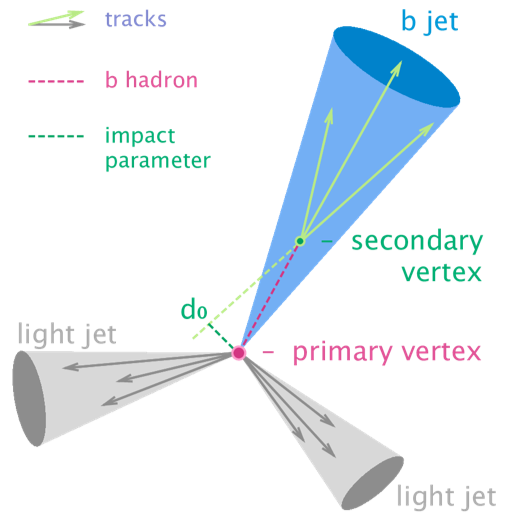
\includegraphics[width=0.9\textwidth]{Images/bjet}
  \caption{Representation of a $b$-jet \cite{bjetimage}.}
  \label{fig:bjet}
\end{subfigure}
\begin{subfigure}[b]{0.49\textwidth}
  \centering
  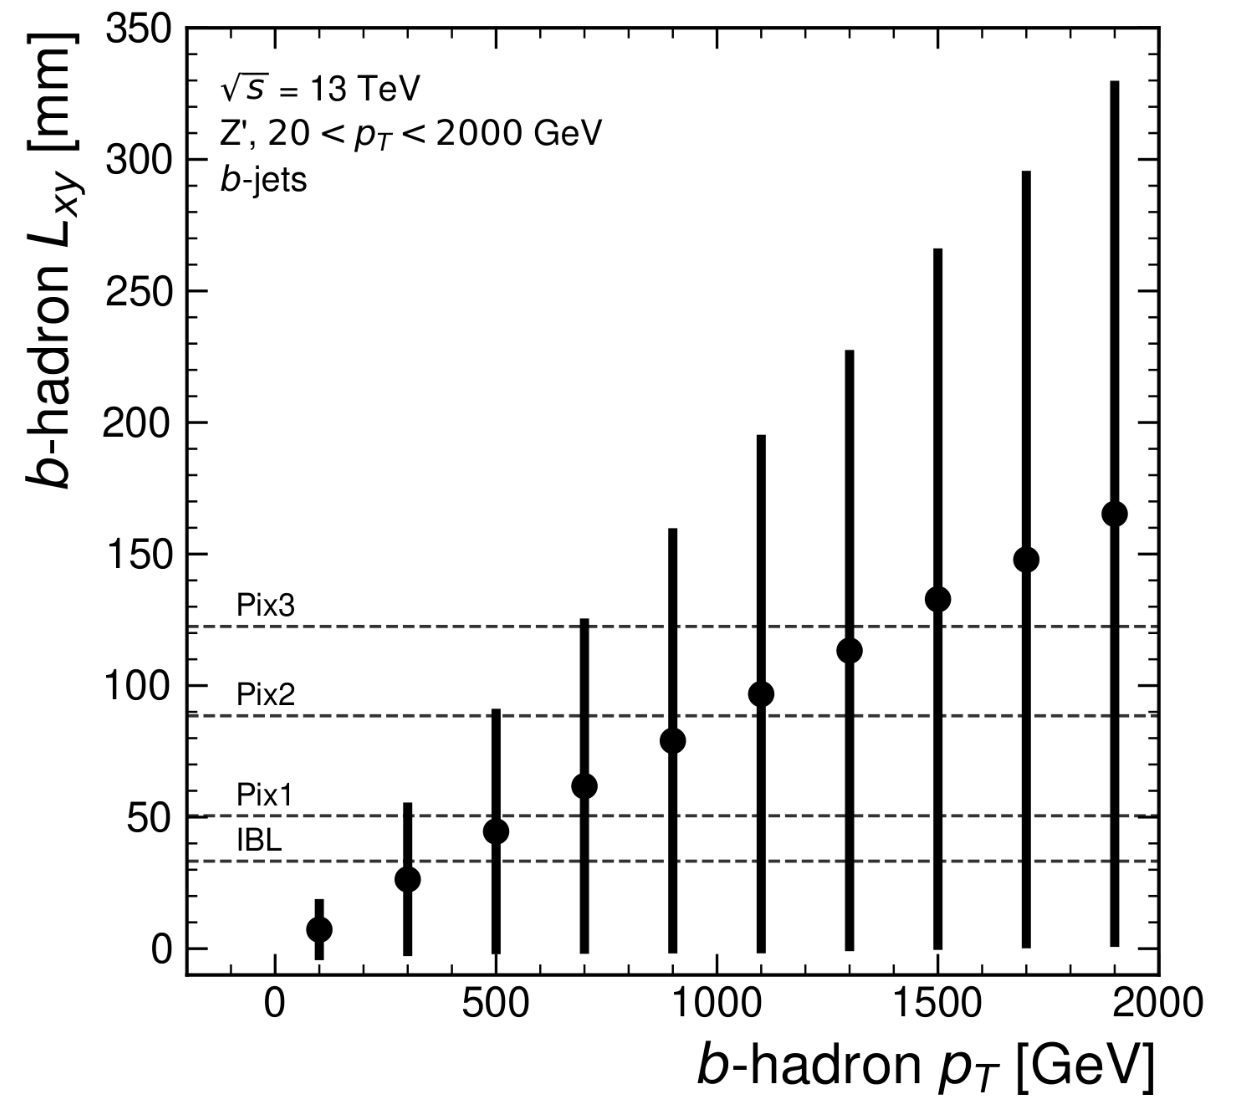
\includegraphics[width=0.98\textwidth]{Images/FTAG/intro/bhaddecay.png}
  \caption{$b$-hadron decay radius as a function of jet $p_T$ reconstructed for $b$-jets in a $Z'$ events with the IBL and pixel layers indicated, from \cite{VanStroud:2869719}. Error bars show the standard deviation of $L_{xy}$ in each $p_T$ bin.} 
  \label{fig:bhaddecay}
\end{subfigure}
\end{figure}

While $b$-jets benefit from an advantageous topology, tagging $c$-jets proves much more challenging as they are at an intermediate scale between light- ($u$, $d$, $s$, and gluons) and heavy flavour jets. A $c$-jet must contain at least one $c$-hadron, from either a $D$-meson (e.g., $D^+=c\bar{d}$, $D^-=d\bar{c}$, $D^0=c\bar{u}$) or a $c$-baryon (e.g., $\Lambda_c^+:udc$). The average decay length for charged (neutral) $D$-mesons, $c\tau_D \sim 300$ $(100)$ $\mu$m \cite{Tanabashi:2018oca}, is smaller than for $b$-hadrons and is harder to resolve with the currently deployed tracker. The decay chain of $b$-hadrons often includes a $c$-hadron, making a clean separation of $c$-jets from $b$-jets harder. Compared to $b$-jets, $c$-jets have a lower final state charged particle multiplicity, on average 4. This lets $\tau$-jets easily being mistaken for $c$-jets, as these leptons can hadronically decay into a similar number of particles to mimic a jet in the detector. For all these reasons, less effort has been historically dedicated to constructing $c$-taggers in ATLAS. The task is however gaining particular attention due to the focus on the challenging $H \rightarrow c\bar{c}$ search \cite{Aaboud:2018fhh, Collaboration:2721696, arXiv:2205.05550}. The focus of this chapter is on the development of novel taggers to identify $b$- and $c$-jet for the ATLAS experiment during the 2020-2024 period, overlaping with the end of Run 2 (2015-2018) analyses and the begining of Run 3 (2022-2026).

\subsection{Flavour Tagging at ATLAS}
In the ATLAS experiment, a choice was made to develop centrally a tagger to be used by the whole collaboration. It relies on a dedicated set of algorithms to perform simultaneously $b$- and $c$-tagging and is continuously improved to meet the requirements of the physics program. Currently, all adopted approaches rely on \gls{dl} methods, given their vastly superior effectiveness. This area of research has been evolving rapidly in recent times due to the community adopting advanced methods from the field of \gls{ai}. As such, various models have been introduced and the last two generations can be split into two categories: 
\begin{enumerate}
  \item The DL1 family are \gls{dl} models built in a hierarchical way. These \gls{dl} methods rely on high-level features reconstructed by sub-algorithms based on physics variables, such as the tracks \glspl{ip}, and the reconstruction of secondary vertices \cite{ATL-PHYS-PUB-2015-022}. The most important models in this family are those including a \gls{dl} sub-model to analyse tracks with either a \gls{rnn} approach for \gls{dl1r} \cite{ATLAS:2017bcq}, leveraging the \gls{rnnip} sub-tagger \cite{ATL-PHYS-PUB-2017-003}, and a Deep Set approaches for \gls{dl1d}, leveraging the \gls{dips} sub-tagger \cite{ATL-PHYS-PUB-2020-014}. This last tagger is, at the moment of writing this thesis, the state-of-the-art deployable tagger for ATLAS in the ATLAS software \cite{ATL-SOFT-PUB-2021-001}. Algorithms from this family were developped for Run 2 of the ATLAS experiment \cite{atlas:FTAGRUN2}, with \gls{dl1d} behind developped towards the end of this data campaign.
  \item The GN family of taggers are built on more advanced \gls{dl} method, as they move away from the hierarchical approach of the DL1 family and directly analyse track and jet information in a unique complex architecture. The GN family is based either on a full Graph Attention Network (\gls{gat}) for \gls{gn1}, and a Transformer encoder for \gls{gn2} \cite{ATL-PHYS-PUB-2022-027, ATL-PLOT-FTAG-2023-01, duperrin2023flavour}. This lighter algorithm pipeline greatly simplifies the maintenance and turnaround time for modification, making the process of updating the taggers nimbler and easier to tailor to specific applications. The GN taggers greatly outperform the DL1 family and represent an exciting area of progress for future analysis requiring precise flavour jets tagging. These methods are being integrated in the ATLAS software stack with objective to be integrated in analyses of the ongoing Run 3 \cite{ATL-SOFT-PUB-2021-001}.  
\end{enumerate}

\begin{figure}[h!]
  \center
  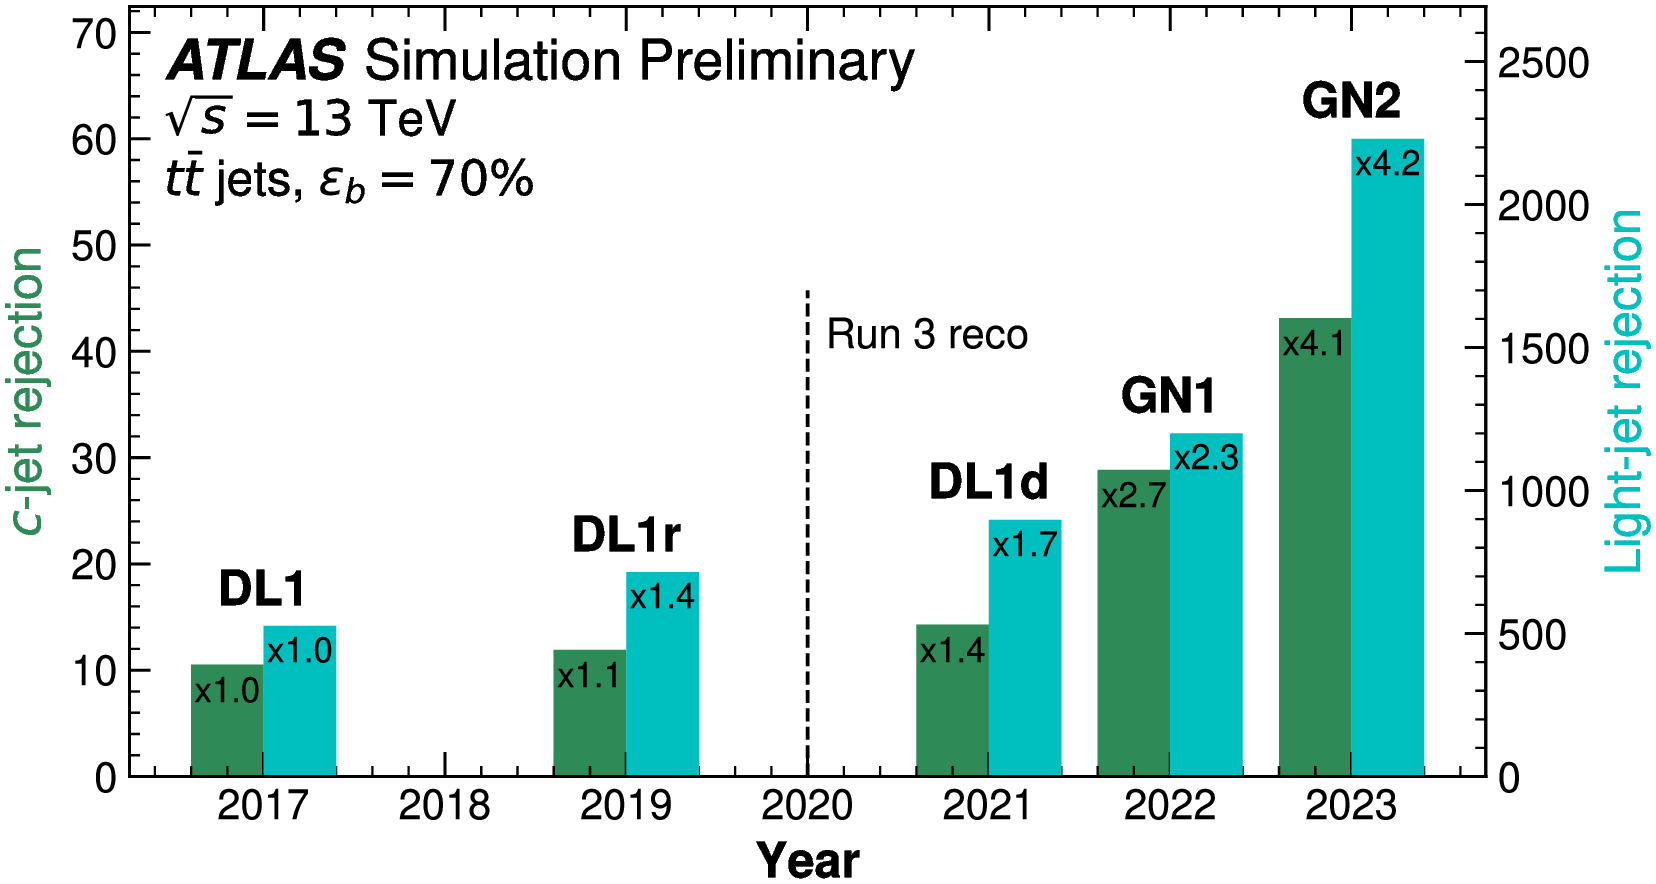
\includegraphics[width=0.8\textwidth]{Images/FTAG/storyFtag.png}
  \caption{Comparison of the performance of flavour tagging models introduced through the years, from \cite{ATL-PLOT-FTAG-2023-01}. Light and $c$-jet rejections are plotted for different taggers at a fixed $b$-jet tagging efficiency of 70\% on a common $t\bar{t}$ evaluation sets. The multiplicative factors in the bars are with respect to the bare DL1 model performance.} 
  \label{fig:storyFtag}
\end{figure}

A historical perspective on the evolution of performance for the different taggers mentioned is presented in Figure \ref{fig:storyFtag}, showing a remarkable continuous increase in light- and $c$-jet rejections at a fixed $b$-tagging efficiency of 70\% on a $t\bar{t}$ dataset. The analysis presented in the latter part of this thesis was carried out in the span of 2021-2024, and was therefore restricted to tools and methods available to the experimental team during this period. As such, due to the need to calibrate the GN taggers as explained latter in Section \ref{chap-calibration} of this chapter, the second family of taggers based on graphs was not yet ready for deployement, making the first family still relevant to explore. Furthemore, some specialised use of flavour taggers and early Run 3 analyses still required the DL1 family, such as the $X_{bb}$ tagger identifying pairs of $b\bar{b}$ and $c\bar{c}$ produced by heavy resonance decays such as a Higgs or a $W$, as described in Section \ref{chap-GN2X}. All the taggers described in this chapter have been integrated in the ATLAS software \cite{ATL-SOFT-PUB-2021-001}. Some early studies of the future performance of the \gls{dl1d} and \gls{gn1} taggers with the updated \gls{itk} detector at the high-luminosity \gls{lhc} as been performed in Ref \cite{ATL-PHYS-PUB-2022-047}.

\subsection{Datasets}\label{ftagdatasets}
The $p_T$ spectrum studied by ATLAS covers a wide range of energies, extending up to 7 TeV. In order to train models able to perform on this large phase space, two datasets are typically combined and described in this section. Each dataset is based from simulated proton-proton collisions at a centre of mass energy $\sqrt{s}$ = 13 TeV. The lower $p_T$ phase space is simulated with the \gls{sm} top-antitop quark pair production $t\bar{t}$ process with at least one $W$ boson produced decaying leptonically, while a \gls{bsm} $Z'$ process is used for the higher momentum region. The latter simulates a modified $Z$ boson from the \gls{sm} with an increased mass to generate a relatively flat jet $p_T$ spectrum of up to 6 TeV. This $Z'$ boson decays in similar proportions to a pair of $b$, $c$, and light-jets. All simulations include realistic effects present in the real data, such as multiple proton-proton interactions per bunch crossing, so-called \glsfirst{pu}, with an average value of $\mu = 40$. Other effects including in the simulations are the detector response from prior and posterior bunch crossing (in-time pile-up) as well the activity from the rest of the event (underlying event). \\

Events in the $t\bar{t}$ samples are simulated using \uppercase{POWHEGBOX V2} generators to next-to-leading (NLO) order in the strong coupling constant $\alpha_s$ \cite{PaoloNason_2004, StefanoFrixione_2007, StefanoFrixione_20072, POWHEGBOX}. The hard scatter matrix element is computed for proton-proton collision with the \uppercase{NNPDF3.0NNLO} set of parton distribution functions (PDF) \cite{PDFLHCrun2}, and the simulated hard scatter events are interfaced with \uppercase{PYTHIA 8.230} \cite{SJOSTRAND2015159} using the A14 parameter tune \cite{ATL-PHYS-PUB-2014-021} and the \uppercase{NNPDF2.3LO} PDFs for the parton shower, hadronisation, and underlying event simulations \cite{BALL2013244}. Studies in Refs \cite{ATL-PHYS-PUB-2016-020, ATL-PHYS-PUB-2020-023} showed these to be the optimal choice to correctly model the top quark $p_T$ and the number of additional jets in the event, with the $h_{\textrm{damp}}$ parameter set at 1.5 the mass of the top-quark $m_{\textrm{top}} = 172.5$ GeV. The $Z'$ events are fully simualted with \uppercase{PYTHIA 8.212}, A14 tune and the \uppercase{NNPDF2.3LO} PDFs. The decays of $b$- and $c$-hadrons are performed by \uppercase{EvtGEN} v1.6.0 \cite{LANGE2001152}. \\

The detector reconstruction effect of ATLAS and the modelling of the interaction between long-lived hadrons and the detector material are simulated with a dedicated software \cite{ATLASSimulationInfra} built on GEANT4 \cite{Agostinelli:602040}. Jets are selected in the phase space region defined by $|\eta| < 2.5$ and $p_T > 20$ GeV, with no overlapping with prompt generator-level $e$ or $\mu$ from the $W$ decay allowed. Pile-up contamination is further reduced by an additional standard selection using the \glsfirst{jvt} algorithm at a tight working point for jets with $p_T < 60$ GeV and $|\eta| < 2.4$ \cite{ATLAS-CONF-2014-018}. Tracks are associated to jets using a $\Delta R$ association cone of width decreasing with $p_T$ ($\Delta R \approx 0.45$ at $p_T =$ 20 GeV and $\Delta R \approx 0.25$ at $p_T > 200$ GeV). Tracks within the cones of several jets are associated to jet with minimal $\Delta R(\textrm{track, jet})$. The label of the jet is inferred from the presence of a truth-level hadron within the cone $\Delta R(\textrm{hadron, jet}) < 0.3$ centred around the jet axis.

\section{DL1 Family of Models: DL1r \& DL1d}
This family of tagger is built with a hierarchical approach, combining low-level algorithms that are independentely optimised into a final \gls{dnn} network of a few layers to output a final prediction. Not all low-level modules are based on \gls{dl}, with some instead directly implementing physics-motivated algorithms. They consist of \cite{Paganini:2289214, atlas:FTAGRUN2}:
\begin{itemize}
  \item \gls{ip} likelihood: IP2D and IP3D are likelihood-ratio templates in 2D and 3D to assign flavour-discriminating weights based, respectively, on the transversal and global impact parameters significance (corresponding to the reweighted \gls{ip} variables by their respective uncertainties) $S_{d_0}$ (35 bins) and $S_{z_0}$ (20 bins) of the tracks, and 14 bins of track catogarisation for IP3D \cite{ATLAS:2017bcq}. For the three flavours, this results in $35 \times 20 \times 14 \times 3 = 29,400$ final bins, which each probability being computed per track. The likelihood assigned to the jet assumes the tracks are independent and is therefore calculated as the product of the per-track likelihoods. A discriminant is derived from the conditional log-likelihood, e.g., $D^b_{IP3D,f} = \sum_{i \in \textrm{tracks}} \log\frac{p_b^i}{p_f^i}$, with $f= c$ or light \cite{ATL-PHYS-PUB-2015-022}.
  \item Track collection analyser: either with \gls{rnnip} \cite{ATL-PHYS-PUB-2017-003} or \gls{dips} \cite{ATL-PHYS-PUB-2020-014}. These are \gls{dl} approaches to extract discrimination information on the set of tracks associated with a jet. These taggers are further described later in this chapter.  
  \item \gls{sv1}: combining a secondary vertex finder and a tagger to offer flavour discrimination information \cite{atlas:FTAGRUN2}. The former, based on the VKalVrt vertex reconstruction package \cite{Kostyukhin:685551}, returns a list of candidate secondary vertices with measured quantities assigned to each vertex. The latter derives jet weights based on discriminative variables and computes properties of the \gls{sv}, such as the mass. 
  \item Jet Fitter: a vertexing algorithm based on a Kalman filter to reconstruct the topology and fit the decay chain \gls{pv} $\rightarrow$ $B$ $\rightarrow$ $D$ with the assumption that the vertices of the weakly decaying B/D-hadrons tend to align with the \gls{pv} \cite{atlas:FTAGRUN2, ATL-PHYS-PUB-2018-025}. 
\end{itemize}

\begin{figure}[h!]
  \centerline{
  \begin{minipage}[c]{0.4\textwidth}
      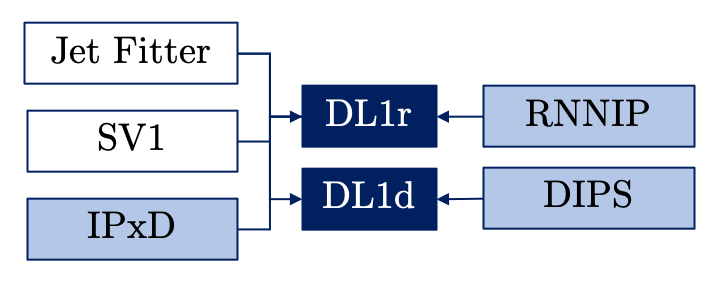
\includegraphics[scale=0.5]{Images/Algorithms}
    \end{minipage}
  \begin{minipage}[c]{0.6\textwidth}
      \caption{The algorithms for flavour tagging at ATLAS. High-level taggers are in dark blue, track-based taggers in light blue and vertex-related taggers in white.}
      \label{fig:algo}
    \end{minipage}
  }
\end{figure}

The outputs of these low-level algorithms, as well as certain jet-related variables, such as $p_T$, are then combined as input to a high-level tagger consisting of a fully-connected \gls{nn} called \gls{dl1r} or \gls{dl1d}, respectively if \gls{rnnip} or \gls{dips} is used. The input vector is typically made of 44-45 features. This high-level tagger outputs three probabilities $p_X$ for the analysed jet to correspond to a $b$-, $c$-, or light--flavour (indicated with the letter $u$) such that $p_b + p_c + p_u = 1$. A $b$-tagging score $D_b$ is then derived by computing a scaled log-likelihood ratio: 
\begin{equation}\label{bdisc}
D_b = \log \frac{p_b}{f^b_c \times p_c + (1 - f^b_c) \times p_u},
\end{equation}
where $f^b_c$ is the charm fraction, a parameter that can be modified to tweak the importance of each flavour. The analogous $c$-tagging score $D_c$ is: 
\begin{equation}\label{cdisc}
D_c = \log \frac{p_c}{f^c_b \times p_b + (1 - f^c_b) \times p_u}.
\end{equation}

A jet is $X$-tagged if the $D_X$ discriminant score is above a set threshold constant $c_{wp}$, defining a \gls{wp} with a unique configuration of signal and background (mis-tag) efficiencies. In this context, the efficiency $\epsilon^X_Y$ for $Y$-flavour jets to be $X$-tagged and the corresponding rejection $\mathcal{R}^X_Y$ are respectively defined as:
\begin{equation}
\epsilon^X_Y = \frac{N^{X-tagged}_{Y-jets}}{N_{Y-jets}} \quad \textrm{and} \quad \mathcal{R}^X_Y = \frac{1}{\epsilon^X_Y},
\end{equation}
where $N^{X-tagged}_{Y-jets}$ and $N_{Y-jets}$ are respectively the number of $X$-tagged $Y$-flavoured jets and the total number of $Y$-flavoured jets. The $f$-rejection is the inverse miss-tagged efficiency of flavour $f$.  \\

These high-level models are trained on \gls{mc} simulated data samples, as mentioned in Section \ref{ftagdatasets}, and need to be calibrated on real data to deliver an unbiased estimate, by deriving \glspl{sf} weights correcting the predictions for each jet as described in Section \ref{chap-calibration}. Uncertainties are derived on the predicted score and passed along to analyses using the tool. The novel algorithm of this family introduced in this work is the \gls{dl1d} tagger, which relies on the \gls{dips} sub-tagger to extract correlations between the tracks.  

\subsection{RNNIP}
The \gls{rnnip} tagger runs on arbitrary-length input sequences made of track features, as ordered by the absolute transverse \gls{ip} significance $|S_{d_0}|$, to extract tagging information from correlations between tracks \cite{ATL-PHYS-PUB-2017-003}. The vector of track features, described in greater details in Table \ref{tab:rnnipVar}, includes the transverse and longitudinal impact parameter significances, the jet $p_T$ fraction carried by the track, the distance between the track and the jet axis, and a learned 2D embedding of the track quality \cite{Paganini:2289214}. It outputs a probability $p_X$ for the jet to belong to flavour $X$ $\in$ [$b$, $c$, light, $\tau$].

\begin{figure}[h!]
  \center
  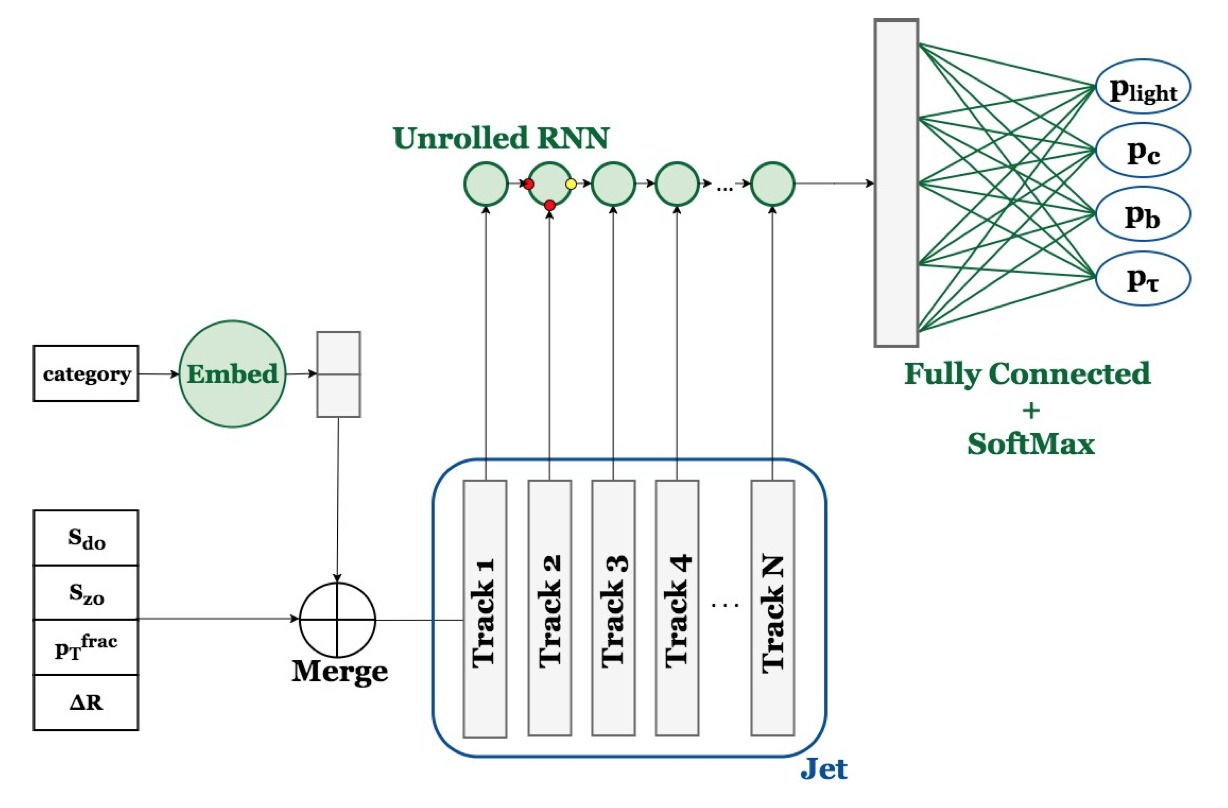
\includegraphics[scale=0.6]{Images/FTAG/rnnip_structure.png}
  \caption{Diagram of the \gls{rnnip} tagger for flavour tagging, from \cite{Paganini:2289214}. The input consists in track features augmented with an embedding of track categories. Tracks are then ordered by absolute transverse \gls{ip} significance and fed through an \gls{lstm} core. The unrolled sequence outputed from this \gls{lstm} is padded to a fixed size and processed by a \gls{dnn} to output the per-flavour probabilities.} 
  \label{fig:rnnipModel}
\end{figure}

The architecture of \gls{rnnip} is a \gls{rnn}-based model leveraging an \gls{lstm} core, as depicted in Figure \ref{fig:rnnipModel}. The arbitrary-length sequence fed as input is mapped by the \gls{lstm} cell with a 100-unit hidden layer into a 50-dimensional vector. This vector is then processed by a 20-unit fully-connected feed-forward neural network outputing the per-flavour probabilities by computing the softmax of the last layer's output. To avoid overfitting, a dropout value of 0.2 is applied to the \gls{lstm} cell. 

\begin{table}[h]
  \begin{center}
      \begin{tabular}{C{3cm}|C{13cm}} 
      	 \hline \hline
          Track Variables & Description  \\ \hline \hline
          $S_{d_0}$      & Lifetime signed transverse \gls{ip} significance $d_0 / \sigma_{d_0}$, with $d_0$ the transverse \gls{ip} - the transverse distance from the \gls{pv} to the point of closest approach (perigee) of the track - and $\sigma_{d_0}$ the error on $d_0$. If the perigee is in front (behind) the \gls{pv} with respect to the jet direction, the sign is positive (negative). \\ \hline
          $S_{z_0}$      & Lifetime signed longitudinal \gls{ip} significance $z_0 / \sigma_{z_0}$, with $z_0$ the longitudinal \gls{ip} - the longitudinal distance from the \gls{pv} to the perigee of the track - and $\sigma_{z_0}$ the error on $z_0$. A sign is assigned as per the prescription of $S_{d_0}$. \\ \hline
          $p_T^{\textrm{frac}}$   & Fraction of the reconstructed jet $p_T^{\textrm{jet}}$ carried by the track $p_T^{\textrm{frac}} = p_T^{\textrm{track}} / p_T^{\textrm{jet}}$. \\ \hline
          $\Delta R$(track, jet) & Geometrical distance in 2D angle between the track direction and jet axis $\Delta R = \sqrt{(\phi_{\textrm{track}} - \phi_{\textrm{jet}})^2 + (\eta_{\textrm{track} - \eta_{\textrm{jet}}})^2}$. \\ \hline
          Category       & 2D representation of the track quality learnt by an embedding layer. The categorisation is based on the number of observed, expected and missing hits in the different layers of the tracker (silicon pixel and strip detectors) \cite{ATL-PHYS-PUB-2015-022}.  \\ \hline
      \end{tabular}
    \caption{Track variables passed to the initial version of the \gls{rnnip} model \cite{ATL-PHYS-PUB-2017-003}. Later versions removed the category embedding and added the per-track hit information shown for \gls{dips} in Table \ref{tab:dipsVar}.}
    \label{tab:rnnipVar}
  \end{center}
\end{table}

\gls{rnnip} is designed to capture correlations between the tracks of a jet, a rich information explicitely missing from the \gls{ip}-based discriminant of IP2D and IP3D due to the factorisation of the likelihood. Some degree of correlation is expected between tracks, as these can emerge from the same secondary or tertiary vertex of the displaced decay in $b$- and $c$-jets. It removes the cumbersome procedure to built likelihood templates, which demands large amount of data to scale to finer bin resolution and is computationally expensive due to the number of bins scaling exponentially with the number of variables. Early tests showed that \gls{rnnip} is effective at building a discriminant, delivering superior performances to the \gls{ip}-based approaches with only $\sim$40 \% of the parameters - 11,636 trainable parameters for \gls{rnnip} \cite{Paganini:2289214}.

\subsection{DIPS}
The \gls{dips} tagger, based on the Deep Set architecture \cite{NIPS2017f22e4747} and depicted in Figure \ref{fig:dipsModel}, is a \gls{gnn}-based alternative approach to \gls{rnnip} to model the correlations between an arbitrary number of tracks \cite{ATL-PHYS-PUB-2020-014}. As introduced in Chapter \ref{chapter-GNN}, such a model is composed of two fully-connected feed-forward neural network. A first \gls{dnn} called the \textit{track network} $\Phi$ maps each individual track feature vector - similar to the input of \gls{rnnip} - to a latent space representing the nodes of a graph. The representations of each track in this latent space are then pooled by a simple summation operation - representing the unweighted edges of a fully connected graph - and given as input to a secondary \gls{dnn}, called the \textit{jet network} $F$, outputting the predicted probability $p_X$ for the jet to belong to flavour $X$ $\in$ [$b$, $c$, light, $\tau$]. This last network represents the global attribute of the graph $u$, in the notation of Chapter \ref{chapter-GNN}. 
In summary, \gls{dips} computes the following equation on the set of track features $\{ p_i \}$, with $i = 1, ..., N$ for arbitrarily-sized jets of $N$ tracks:
\begin{equation}
  DIPS( \{p_1, ..., p_N \} ) = F\left( \sum_{i=1}^N \Phi(p_i) \right),
\end{equation}
to output the per-flavour probabilities. The separation of computation into a per-track embedding and a per-jet processing after a size-indepent pooling performed by the sumation operator allows the model to process unordered sets of variable size. The track features used as inputs are described in Table \ref{tab:dipsVar}, with only the top 15 tracks as ranked by decreasing $S_{d_0}$ being kept.

\begin{figure}[h!]
  \center
  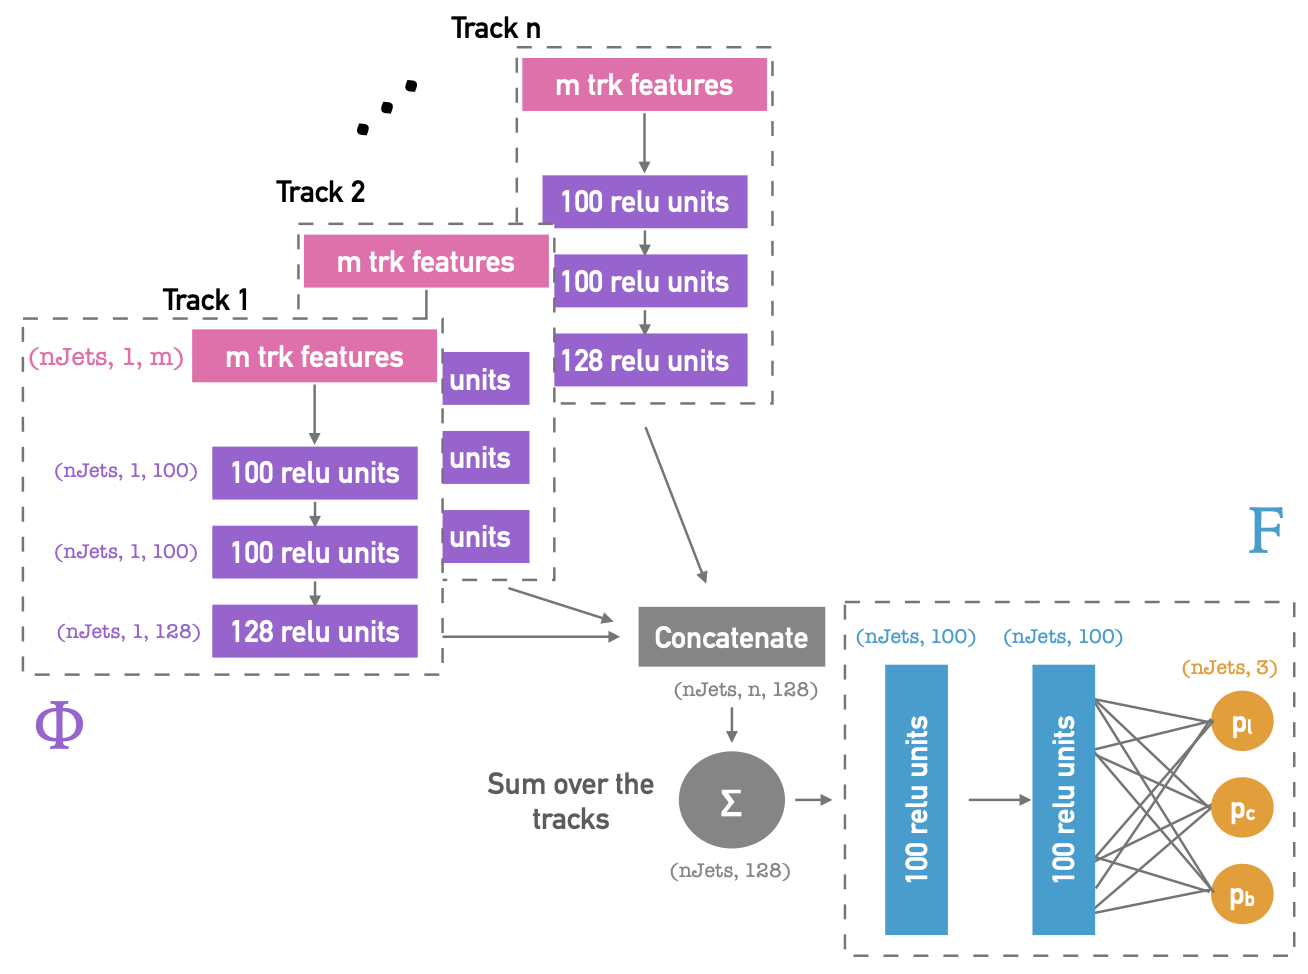
\includegraphics[scale=0.6]{Images/FTAG/dips_structure.png}
  \caption{Diagram of the \gls{dips} tagger for flavour tagging, from \cite{ATL-PHYS-PUB-2020-014}. The input consists in a set of $N$ tracks each represented by a feature vector. Each track is embedded by a \gls{dnn} track network $\Phi$ into a fixed-dimension vector. All embedded track vectors are then pooled by summation to a fixed-size vector. The last step is to process this vector with another \gls{dnn} jet network $F$ outputing the per-flavour probabilities. The number and width of layers presented here are the nominal architecture.} 
  \label{fig:dipsModel}
\end{figure}

\begin{table}[h]
  \begin{center}
      \begin{tabular}{C{3cm}|C{13cm}} 
      	 \hline \hline
          Variables & Description  \\ \hline
          $S_{d_0}$      & Lifetime signed transverse \gls{ip} significance $d_0 / \sigma_{d_0}$, with $d_0$ the transverse \gls{ip} - the transverse distance from the \gls{pv} to the point of closest approach (perigee) of the track - and $\sigma_{d_0}$ the error on $d_0$. If the perigee is in front (behind) the \gls{pv} with respect to the jet direction, the sign is positive (negative). \\ \hline
          $S_{z_0}$      & Lifetime signed longitudinal \gls{ip} significance $z_0 / \sigma_{z_0}$, with $z_0$ the longitudinal \gls{ip} - the longitudinal distance from the \gls{pv} to the perigee of the track - and $\sigma_{z_0}$ the error on $z_0$. A sign is assigned as per the prescription of $S_{d_0}$. \\ \hline
          $\log p_T^{\textrm{frac}}$   & Logarithm of the fraction of the reconstructed jet $p_T^{\textrm{jet}}$ carried by the track $\log p_T^{\textrm{frac}} = \log p_T^{\textrm{track}} / p_T^{\textrm{jet}}$. \\ \hline
          $\log \Delta R$(track, jet) & Logarithm of the geometrical distance in 2D angle between the track direction and jet axis $\log \Delta R = \log \sqrt{(\phi_{\textrm{track}} - \phi_{\textrm{jet}})^2 + (\eta_{\textrm{track} - \eta_{\textrm{jet}}})^2}$. \\ \hline
          IBL hits      & Number of hits recorded in the \gls{ibl} - 0, 1, or 2. \\ \hline
          PIX1 hits       & Number of hits in the innermost pixel layer, after the \gls{ibl} - 0, 1, or 2.  \\ \hline
          Shared IBL hits & Number of hits in the \gls{ibl} that are shared by more than one track. \\ \hline
          Split IBL hits  & Number of split hits in the \gls{ibl}, that are created by multiple charged particles. \\ \hline
          nPixHits        & Total number of hits in all the pixel layers.\\ \hline
          Shared pixel hits & Number of shared hits in the pixel layers.\\ \hline
          Split pixel hits  & Number of split hits in the pixel layers.\\ \hline
          nSCTHits          & Total number of hits in the \gls{sct} layers. \\ \hline
          Shared SCT hits   & Number of shared hits in the \gls{sct} layers.\\ \hline \hline
      \end{tabular}
      \caption{Track variables passed to the \gls{dips} model and later versions of the \gls{rnnip} model \cite{ATL-PHYS-PUB-2020-014}. Compared to the initial \gls{rnnip} variables of Table \ref{tab:rnnipVar}, the $p_T^{\textrm{frac}}$ and $\Delta R$ are passed as log values to reduce the magnitude of the long tail observed at large values and improve the training time. Shared hits are hits used by multiple tracks without being classific as split by a dedicated cluster-splitting \gls{nn} \cite{ATLAS-tracks-algo}.}
    \label{tab:dipsVar}
  \end{center}
\end{table}

This approach has several advantages over \gls{rnnip}, mainly the physically motivated permutation-invariance of the input and the improved training and evaluation time thanks to a more parallelisable architecture, as the track embedding performed by $\Phi$ can be massively parallalised on \gls{gpu}. These motivations are translated in an appreciable performance delivered by \gls{dips}, which is observed to globally outpeform version of \gls{rnnip} using the same variables, while operating at a reduced computational cost \cite{ATL-PHYS-PUB-2020-014}. The performance can be assessed from Figure \ref{fig:dipsrnnipPerf}, presenting the \gls{roc} curves for baselines trainings of \gls{dips} and \gls{rnnip} in terms of light- and $c$-rejection for $b$-jet tagging on the same held-out $t\bar{t}$ evaluation sample.

\begin{figure}[h!]
  \centering
  \begin{subfigure}[b]{0.48\textwidth}
      \centering
      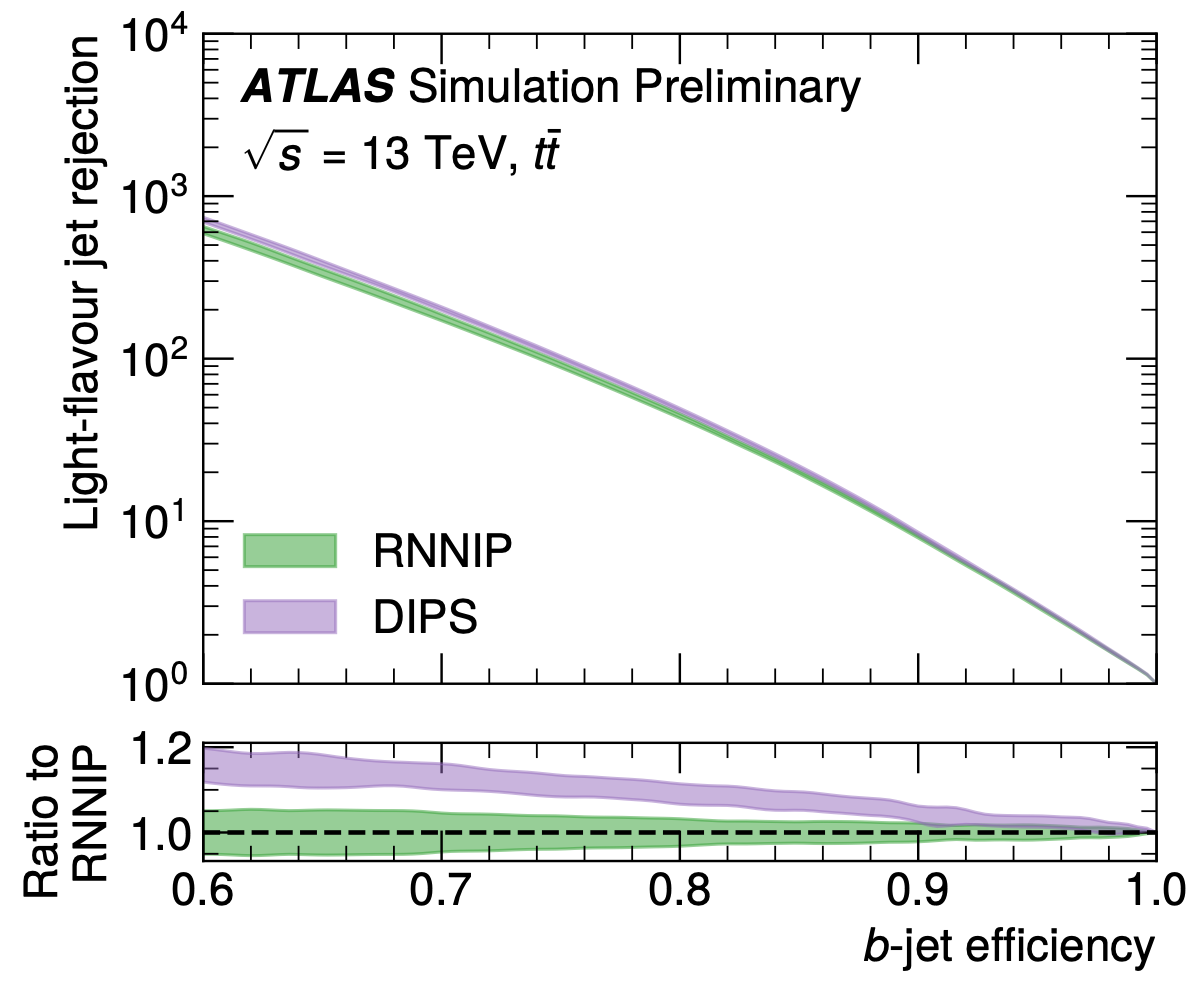
\includegraphics[width=0.98\textwidth]{Images/FTAG/dipsrnnipL.png}
      \caption{Light-rejection.} 
      \label{fig:dipsrnnipPerfL}
  \end{subfigure}
  \hfill
  \begin{subfigure}[b]{0.48\textwidth}
      \centering
      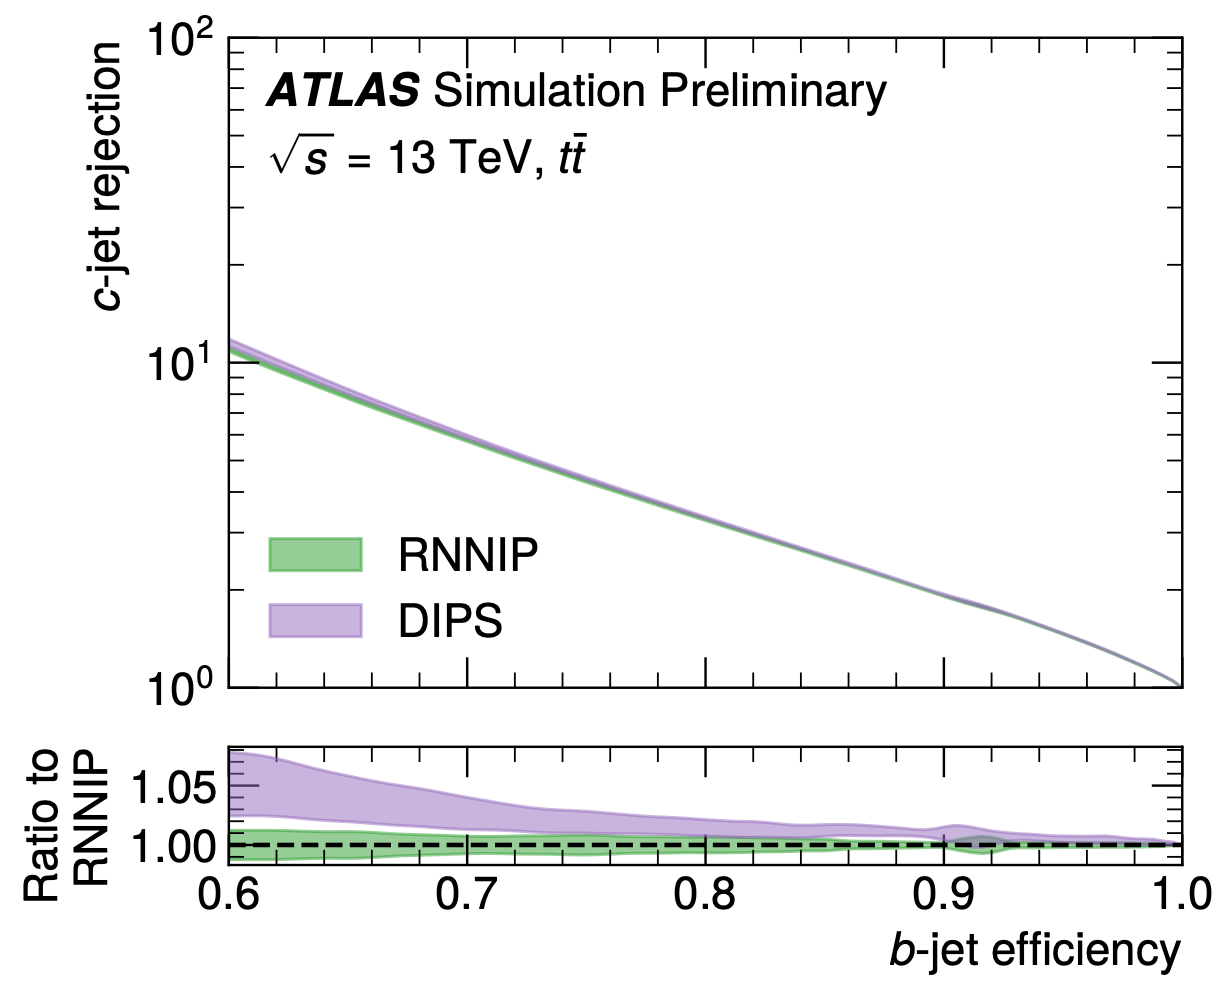
\includegraphics[width=0.98\textwidth]{Images/FTAG/dipsrnnipC.png}
      \caption{$c$-rejection.} 
      \label{fig:dipsrnnipPerfC}
  \end{subfigure}
  \caption{Light- (left) and $c$-rejection (right) as a function of $b$-jet tagging efficiency for \gls{rnnip} (green) and \gls{dips} (purple), taken from \cite{ATL-PHYS-PUB-2020-014}. Each curve and error bands show, respectively, the mean and standard deviation of the rejections for 5 trainings per algorithm. The bottom panel shows the ratio with respect to \gls{rnnip}, showing a clear performance gain for \gls{dips} at all $b$-jet efficiency considered.}
  \label{fig:dipsrnnipPerf}
\end{figure} 

The training times on the same \gls{gpu} hardware for a 48k parameters \gls{dips} model is estimated to take 78 $\pm$ 4 seconds per epoch - averaging over 5 seeds - while a 47k parameters \gls{rnnip} requires roughly thrice as much, 241 $\pm$ 14 seconds per epoch \cite{ATL-PHYS-PUB-2020-014}. The faster training time allowed the Collaboration to focus on optimisation studies of the hyperparameters. The optimisation campaign focused on three aspects of the \gls{dips} network: the architecture of the two \gls{nn}, the track selection, and the set of trac features used as input in addition to those of Table \ref{tab:dipsVar}. Regarding architecture, a grid search over various possible values for the number of layers in $\Phi$ and $F$, number of nodes, and the dimension of the track embedding space showed no significant performance change. The selected architecture is:
\begin{itemize}
  \item Track network $\Phi$: three layers of 100, 100, and 128 units applied to each track. 
  \item Jet network $F$: four layers of size 100, 100, 100, 30 before the final output of size dictated by the number of flavour to identify. 
\end{itemize}
To regularise and avoid overfitting, both batch normalisation and dropout were tested with the former observed to give better results. \\ 

The second optimisation step however uncovered that a variation to the track selection does offer opportunities for improved performance. Jets are reconstructed with the anti-kT algorithm with a radius of R = 0.4. For \gls{rnnip}, IP2D, and IP3D, the selected tracks must pass the following quality selection: $\geq$ 7 hits in the silicon layers, $\leq$ 2 missing hits in the silicon layers, $\geq$ 1 hit in the pixel detector, $\leq$ 1 hit shared by multiple tracks, $p_T$ > 1 GeV, $|d_0|$ < 1 mm, and $|z_0 \textrm{ sin}(\theta)|$ < 1.5 mm. For \gls{dips}, a looser track selection increasing the acceptance of the last three cuts was studied, modifying the nominal selection in the following way: $p_T$ > 0.5 GeV, $|d_0|$ < 3.5 mm, and $|z_0 \textrm{ sin}(\theta)|$ < 5 mm \cite{ATL-PHYS-PUB-2020-014}. Loosening the selection and keeping the top 25 tracks as ranked by decreasing $S_{d°0}$ to capture more tracks from heavy flavour decays was observed to lead to a significant improvement in performance for jets with a $p_T < 250$ GeV for \gls{dips}. From an \gls{ml} viewpoint, a larger set of input information with more noise can still prove beneficial if the underlying model is complex enough to capture useful features in the noisy data, that would otherwise be erased by a more stringent selection. The performance gain from this loosened selection-trained \gls{dips} is displayed in the \gls{roc} curves of Figure \ref{fig:dipsOptRoc}. \\

\begin{figure}[h!]
  \centering
  \begin{subfigure}[b]{0.48\textwidth}
      \centering
      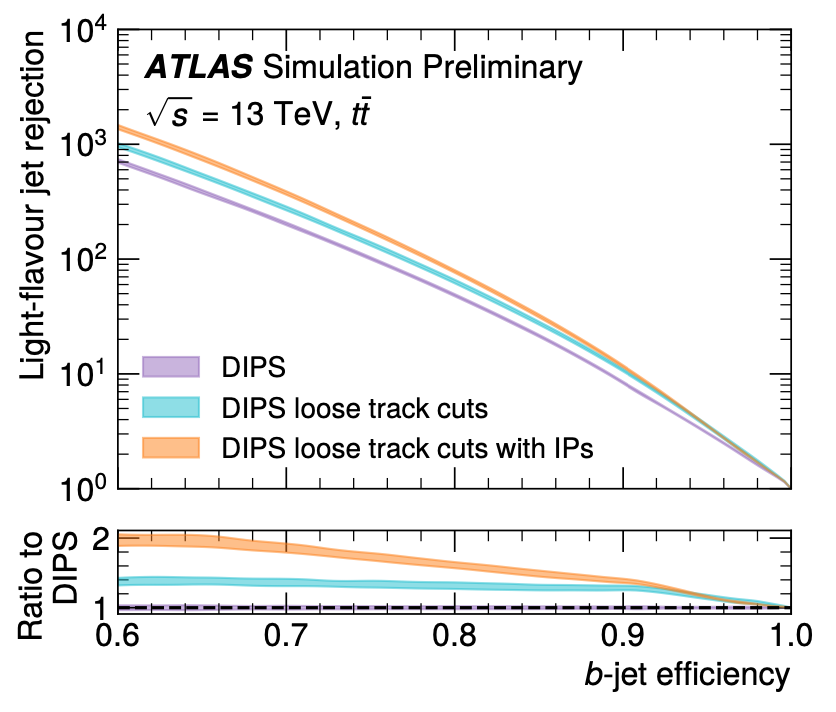
\includegraphics[width=0.98\textwidth]{Images/FTAG/dipsOptL.png}
      \caption{Light-rejection.} 
      \label{fig:dipsOptRocL}
  \end{subfigure}
  \hfill
  \begin{subfigure}[b]{0.48\textwidth}
      \centering
      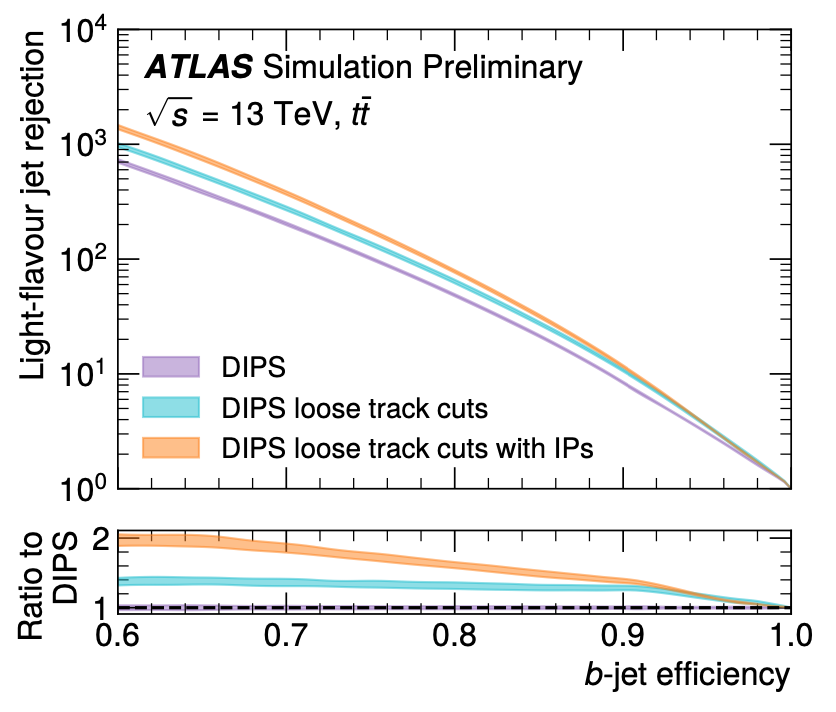
\includegraphics[width=0.98\textwidth]{Images/FTAG/dipsOptL.png}
      \caption{$c$-rejection.} 
      \label{fig:dipsOptRocC}
  \end{subfigure}
  \caption{Light- (left) and $c$-rejection (right) as a function of $b$-jet tagging efficiency for different \gls{dips} model, with the baseline (nominal) \gls{dips} in purple, the loosened track selection in blue, and the fully optimised \gls{dips} in orange, from \cite{ATL-PHYS-PUB-2020-014}. The curve and error bands show, respectively, the mean and standard deviation of the rejections for 5 trainings per algorithm with different initial random seed. The bottom panel shows the ratio with respect to the baseline \gls{dips}, showing a clear performance gain from the two steps optimisation procedure at all $b$-jet efficiency considered.}
  \label{fig:dipsOptRoc}
\end{figure} 

Furthemore, clear benefits are obtained when adding additional track features as input on top of the looser selection, as shown by the orange curve of Figure \ref{fig:dipsOptRoc}, which plots the performance of a loose track selection \gls{dips} trained with the per-track \gls{ip} parameters $d_0$ and $z_0$ in addition to the features of Table \ref{tab:dipsVar}.

\begin{figure}[h!]
  \center
  \begin{minipage}[c]{0.7\textwidth}
    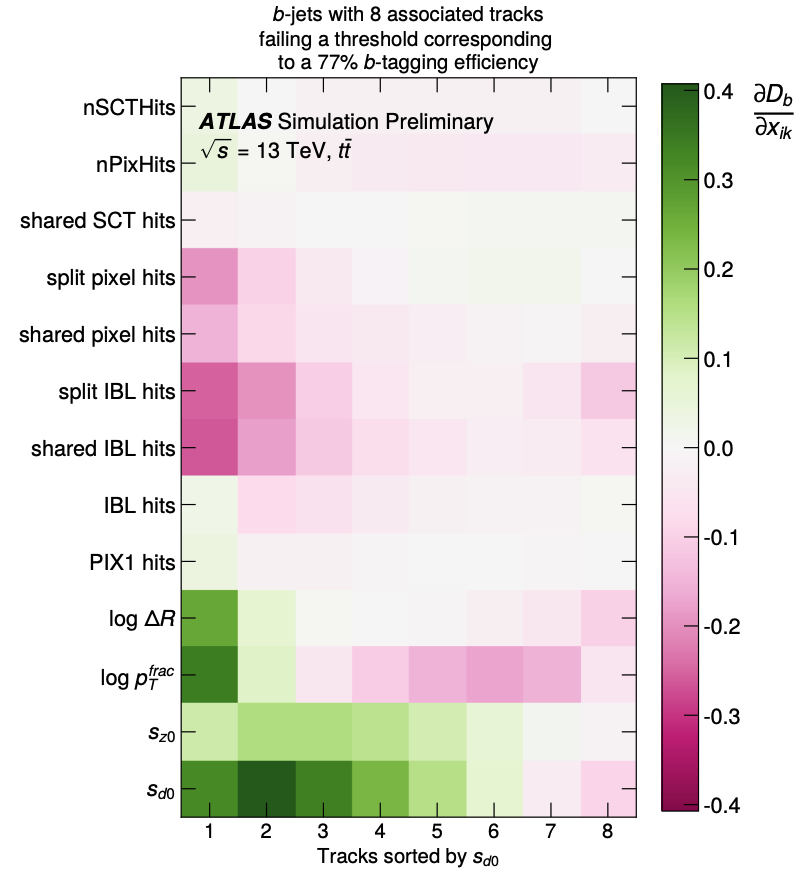
\includegraphics[width=\textwidth]{Images/FTAG/dipsSaliency.png}
  \end{minipage}
  \begin{minipage}[c]{0.25\textwidth}
    \caption{Saliency map for $b$-tagging with 8 tracks sorted by $|S_{d_0}|$, showing the gradient of the discrimant $D_b$ with respect to the track features $x_{ik}$ displayed on the $y$-axis \cite{ATL-PHYS-PUB-2020-014}.} 
  \label{fig:dipsSaliency}
  \end{minipage}
\end{figure}

How does \gls{dips} work? Interpretability of machine learning models is an active area of research. Several effective approaches exist to gauge the importance of the input on the prediction, such as Shapley values. Figure \ref{fig:dipsSaliency} presents an alternative technique called \textit{saliency maps} \cite{Simonyan2013DeepIC}. Using the $b$-tagging discriminant $D_b$ of Equation \ref{bdisc} at a fixed efficiency of 77\%, the average importance of each feature in the track inputs is assessed by averaging the gradient of the discriminant with respect to the track feature over a set of $N$ jets with strictly 8 associated tracks failing the threshold:
\begin{equation}
  \frac{\partial D_b}{\partial x_{ik}} = \frac{1}{N} \sum_{j=1}^N \frac{\partial D_b^{j}}{\partial x_{ik}^{j}},
\end{equation} 
where $i$ indexes the 8 tracks, $j$ indexes the jet in the sample of size $N$, $x_{ik}$ is the $k^{th}$ feature of the $i^{th}$ jet \cite{ATL-PHYS-PUB-2020-014}. This process effectively indicates the linear sensitivity of the discriminant on the track features. Using the saliency map, one can infer what features to modify to correct the failed tagged assigned to the $b$-jets sample. The most sensitive parameters are measured to be the \gls{ip} significances of the first five tracks, and the logarithm of the $p_T^{\textrm{frac}}$ and $\Delta R$ of the track with largest $|s_{d_0}|$. This observation is physically motivated by the dynamic of the harder fragmentation of $b$-quarks, compared to light- and $c$-quarks. Negative gradients are measured for shared and split hits observables, translating into a further incorrect discriminant under linear change of these features. This is also physically motivated, as higher count typically trace back to denser environment where random combinations of hits to form tracks are more likely. However, total hit counts in the different tracker layers have a small positive impact, as these correlate with the reconstruction of the \gls{ip} parameters.

\subsection{Training of DIPS with Variable Radius Jets for Run 3}\label{chapter:dipsVRtrain}
The physics program of the ATLAS Collaboration covers a wide range of analyses, targeting different topologies and processes at different energies. With respect to flavour tagging, a particularly relevant aspect is the energy or tranverse momenta of the jets to label. Indeed, flavour tagger are extremely sensitive to the dynamic of the underlying events. At higher energies, corresponding to higher momenta of the hadronised quark or gluon, the jet constituents emenating from the decaying parton tend to be more collimated in the same direction, as they have to share a high initial energy between themselves. This topology confends tracks and blends the rich internal jet dynamics in the measured signature, making tracks separation and secondary or tertiary vertex identification more difficult. Analyses targeting jets from hadronic or semileptonic decays of heavy particles, such as the top $t$-quark, Higgs, or the gauge bosons $W/Z$, can easily produce such highly energetic or \textit{boosted} jets.  \\

So far in this chapter, mentions of ``jets'' were always referring to the object as reconstructed by the anti-$k_T$ algorithm with a fixed radius $R = 0.4$ applied to PFLow objects, as introduced in Chapter \ref{chapter-ATLAS}. This reconstruction method proves robust in the hadron collider setting as it both leads to suitably-shaped jet structure and \gls{pu}-removing properties. This fixed radius however becomes a hurdle for boosted jet, as their average radius decreases with energy due to the collimation of the jet components. Indeed, the angular separation $\Delta R = \sqrt(\Delta\eta^2 + \Delta \phi^2)$ between the products of a decaying particle $X$ of large mass $m_X$ scales inversely to the transverse momentum \cite{ATLAS:largeRjet}: 
\begin{equation}\label{eq:sizeJet}
  \Delta R \approx \frac{2 m_X}{p_T^X}.
\end{equation}
At low $p_T^X$, the individually produced particle from the decay are sufficiently separated to be reconstructed as individual objects, hence the \textit{resolved} regime label \cite{ATLAS:2016hcf}. For example, a non-boosted Higgs decaying to a $b\bar{b}$ pair can be reconstructed as two $b$-jets with small $R$. At higher momentum however, the content of the decay is collimated and overlaps: this is the \textit{boosted} regime. The decaying particle $X$ in such a regime is typically reconstructed as a single large radius jets, to catch the different underlying jets, for example with the anti-$k_T$ method with radius $R = 1.0$. Using such a fixed large radius overestimates the size of boosted jets which are easily contaminated by the \gls{pu}, as well as the underlying event and initial-state radiations.  \\

A novel approach to model jets from boosted object decays is to reconstruct them with \gls{vr} jet algorithm \cite{vrJetPaper}, as introduced in Chapter \ref{chapter-ATLAS}. \gls{vr} jets have a size that scales with the inverse of the reconstructed jet momentum, thus correctly following the expected dynamic of Equation \ref{eq:sizeJet}. Such a significant change to the jet reconstruction is bound to have an impact on algorithms learning structure from the jet contents, as is the case of all deep learning-based taggers presented in this chapter. These models have therefore to be fine-tuned seperately to this new jet-type for optimal performance, which is the focus of this section. \\  % Chapter with VR JET

For the \gls{vr}-training, the dataset is composed of three samples simulating proton-proton collisions at $\sqrt{s} = 13$ with the following fractions:
\begin{enumerate}
  \item 85 \% of jets are sampled from the $t\bar{t}$ with a maximal $p_T$ of 400 GeV. At least one of the $W$-boson from the $t$-quark is required to decay leptonically.
  \item 7.5\% are sampled from $Z'$ events, where an exotic boson $Z'$ decays as $Z' \rightarrow q\bar{q} \textrm{ or } \tau \bar{\tau}$, with a variable $Z'$ mass to generate a flat $p_T$ spectrum extending the $p_T$-range of the jets studied up to 4 TeV. These jets are required to have a $p_T > 150$ GeV.
  \item 7.5\% are sampled from a simulated graviton process to also increase the range towards higher momenta. These jets are required to have a $p_T > 150$ GeV.
\end{enumerate}

The simulation process is similar to that introduced in Section \ref{ftagdatasets}. Figure \ref{fig:vrjetdist} displays the jet $p_T$ and $|\eta|$ distributions for the hybrid sample as well as the individual samples it is based upon, for a total of 40 $\times$ $10^6$ jets per flavour in \{$b$, $c$, light\}. In order to reach such high statistics, importance sampling is used to over-sample the limited amount of $c$-jets while using all available $b$- and downsampling light-jets. A particularity of the processing is the requirement for the $p_T$ and $|\eta|$ spectra to be equally-distributed for all jet flavours, so that these features arising from inherent physics effects in the specific processes simulated cannot be used by the model to discriminate between flavours. The technique implemented is importance sampling with replacement. It selects jets of different flavours to match a target distribution. The importance sampling weights are derived by first deriving the ratio of the target 2D distribution to the per flavour one. Weights above 1 indicate jets in the $i, j$ bin have to be oversampled, while values lower than 1 indicate the typical downsampling requirement. Jets are then iteratively sampled until the sampled distribution of each flavour individually matches the target distribution. As displayed in Figure \ref{fig:vrjetdisth} for which the target were $b$-jets, the thus constructed distribution as the same $p_T$ and $|\eta|$ distributions for all flavours. This work introduced to the first implementation of the importance sampling method, now widely used to develop flavour tagging tools.  

\begin{figure}[h!]
  \centering
  \begin{subfigure}[b]{0.98\textwidth}
      \centering
      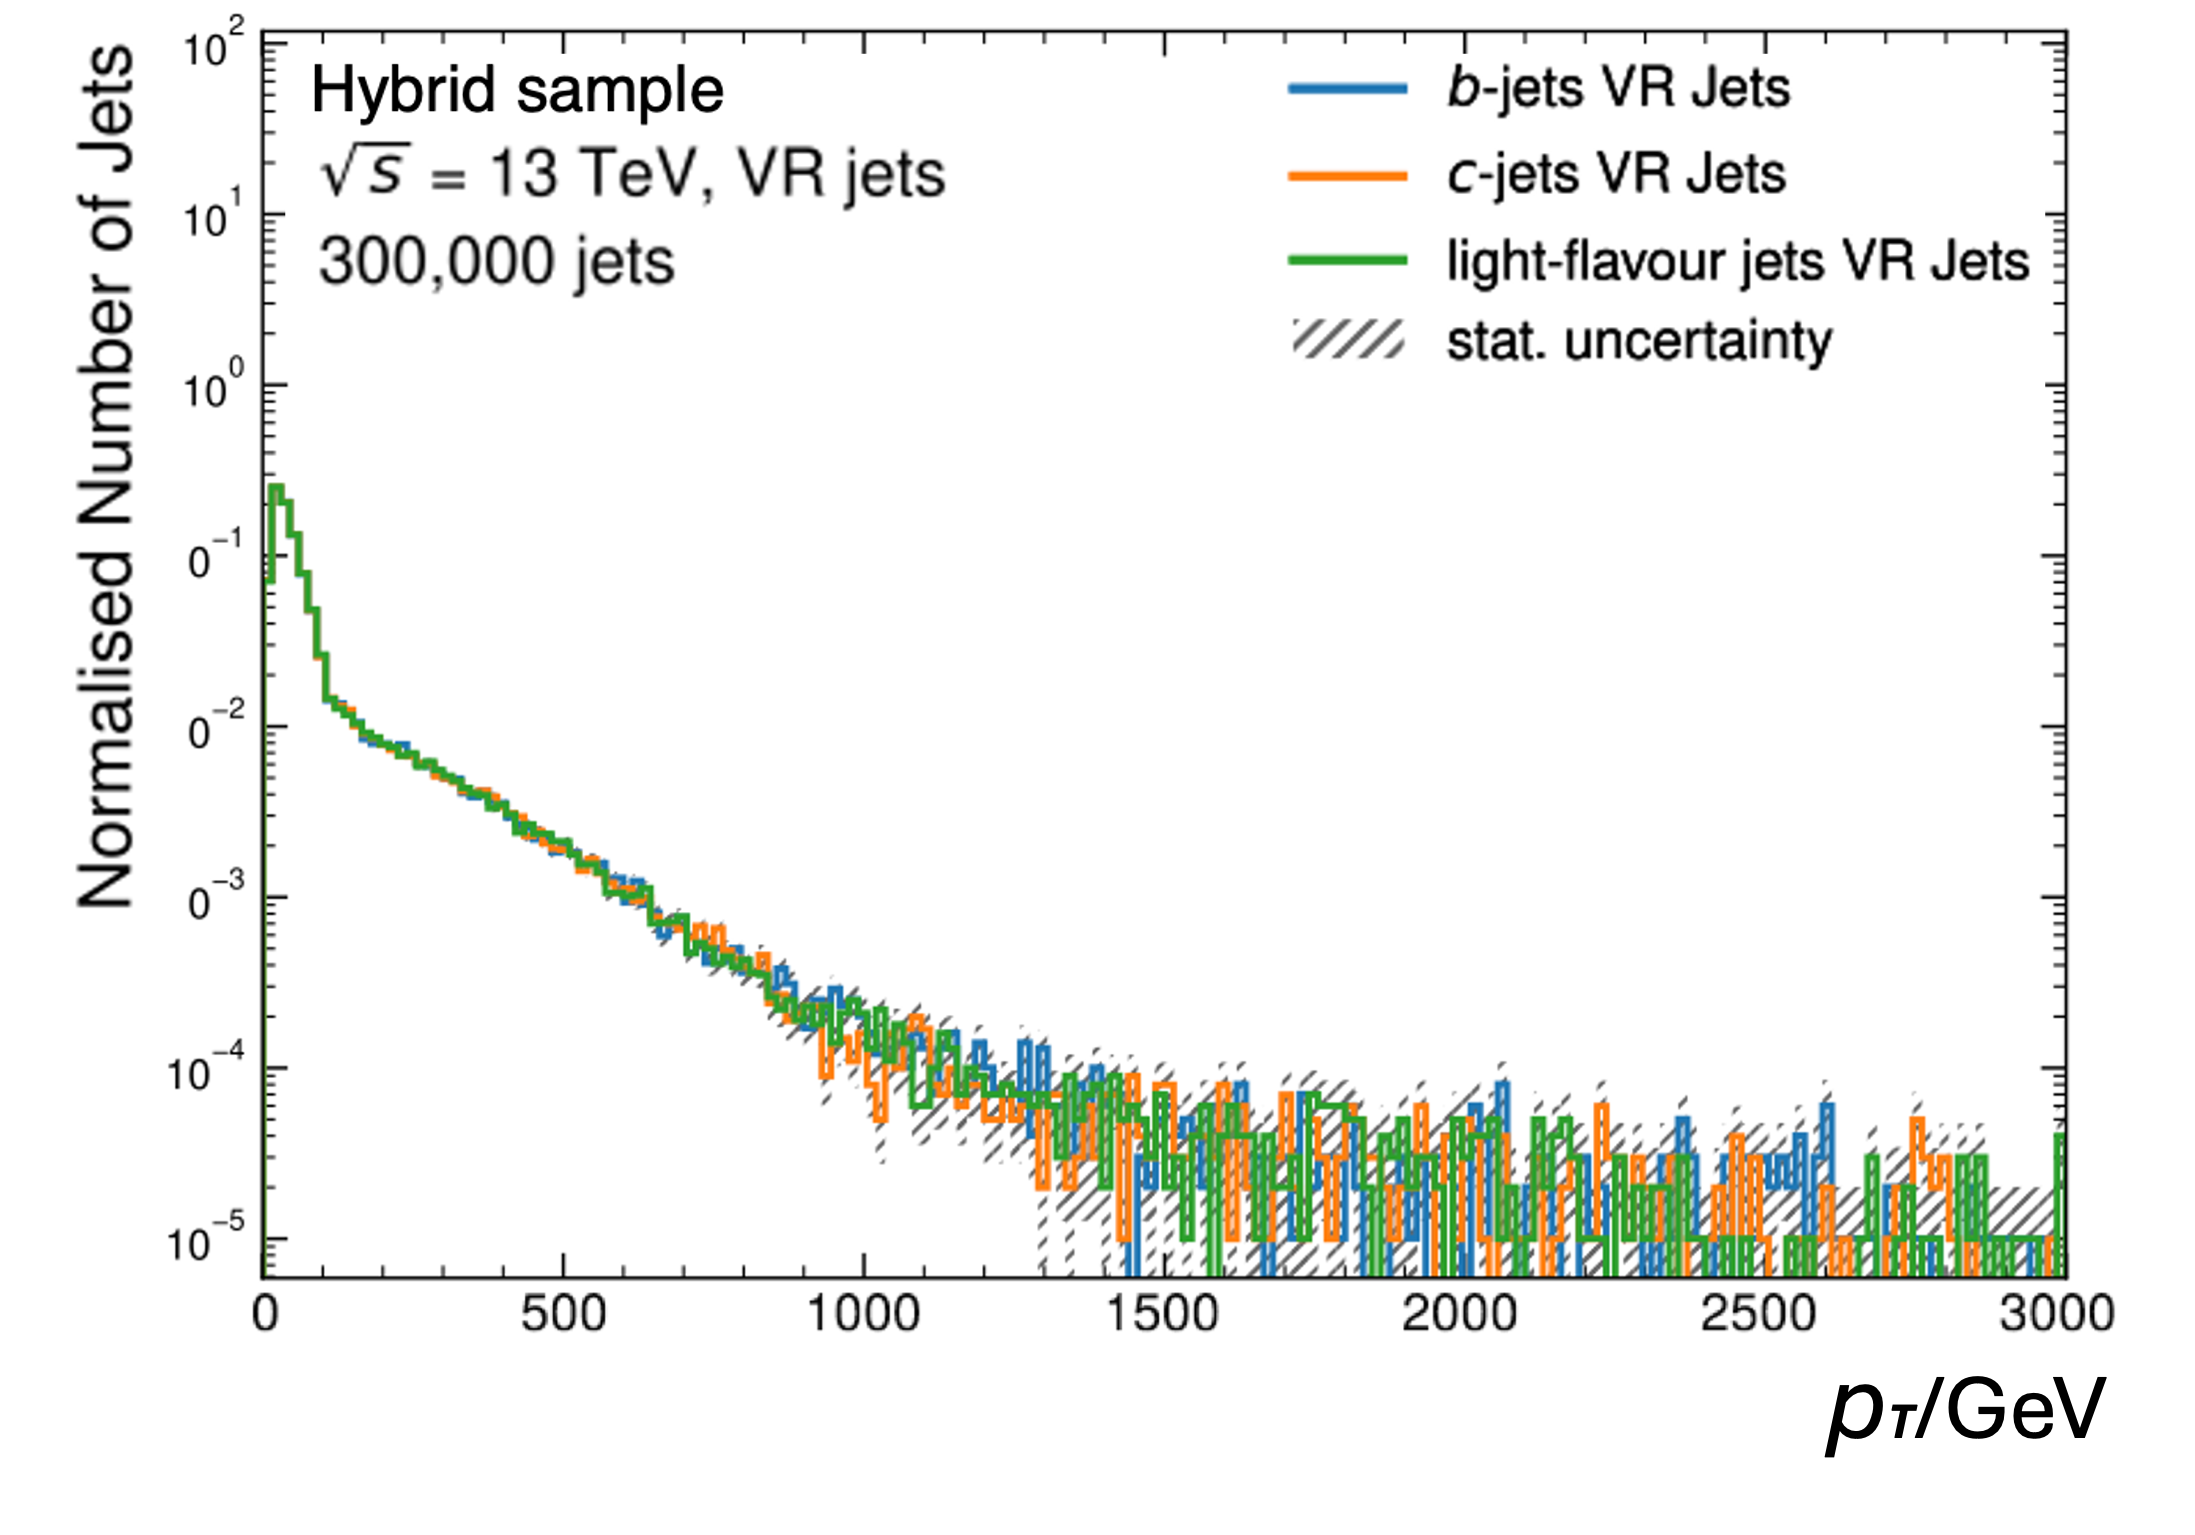
\includegraphics[width=0.48\textwidth]{Images/FTAG/VRDips/JetDist/hspt.png}
      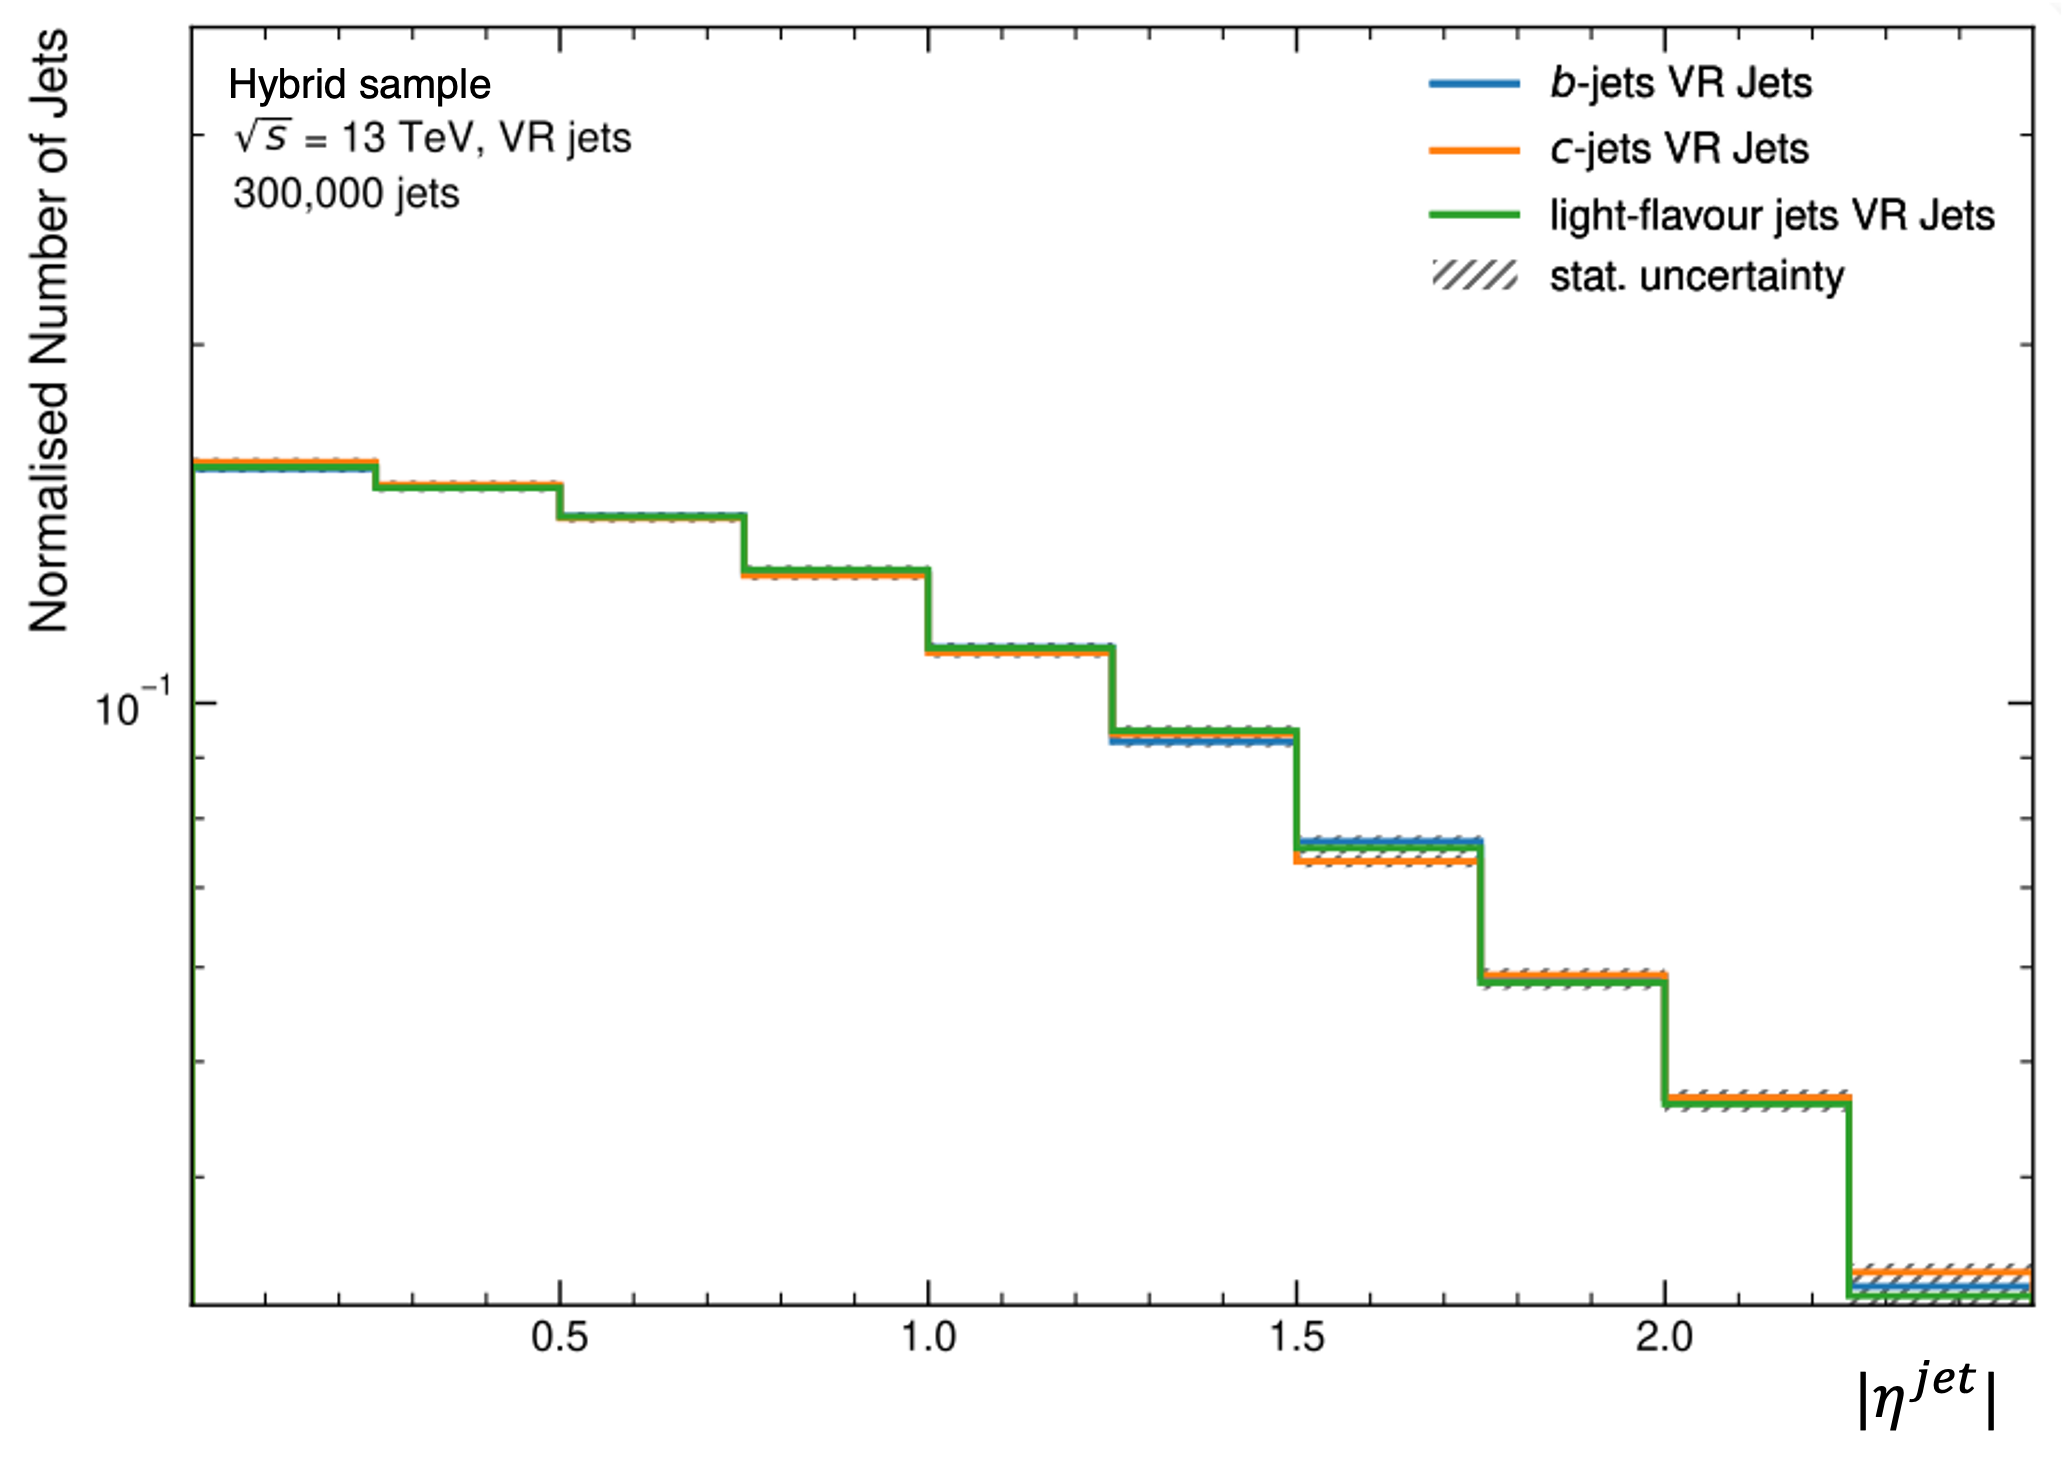
\includegraphics[width=0.48\textwidth]{Images/FTAG/VRDips/JetDist/hseta.png}
      \caption{Hybrid sample.} 
      \label{fig:vrjetdisth}
  \end{subfigure}\\
  \begin{subfigure}[b]{0.98\textwidth}
      \centering
      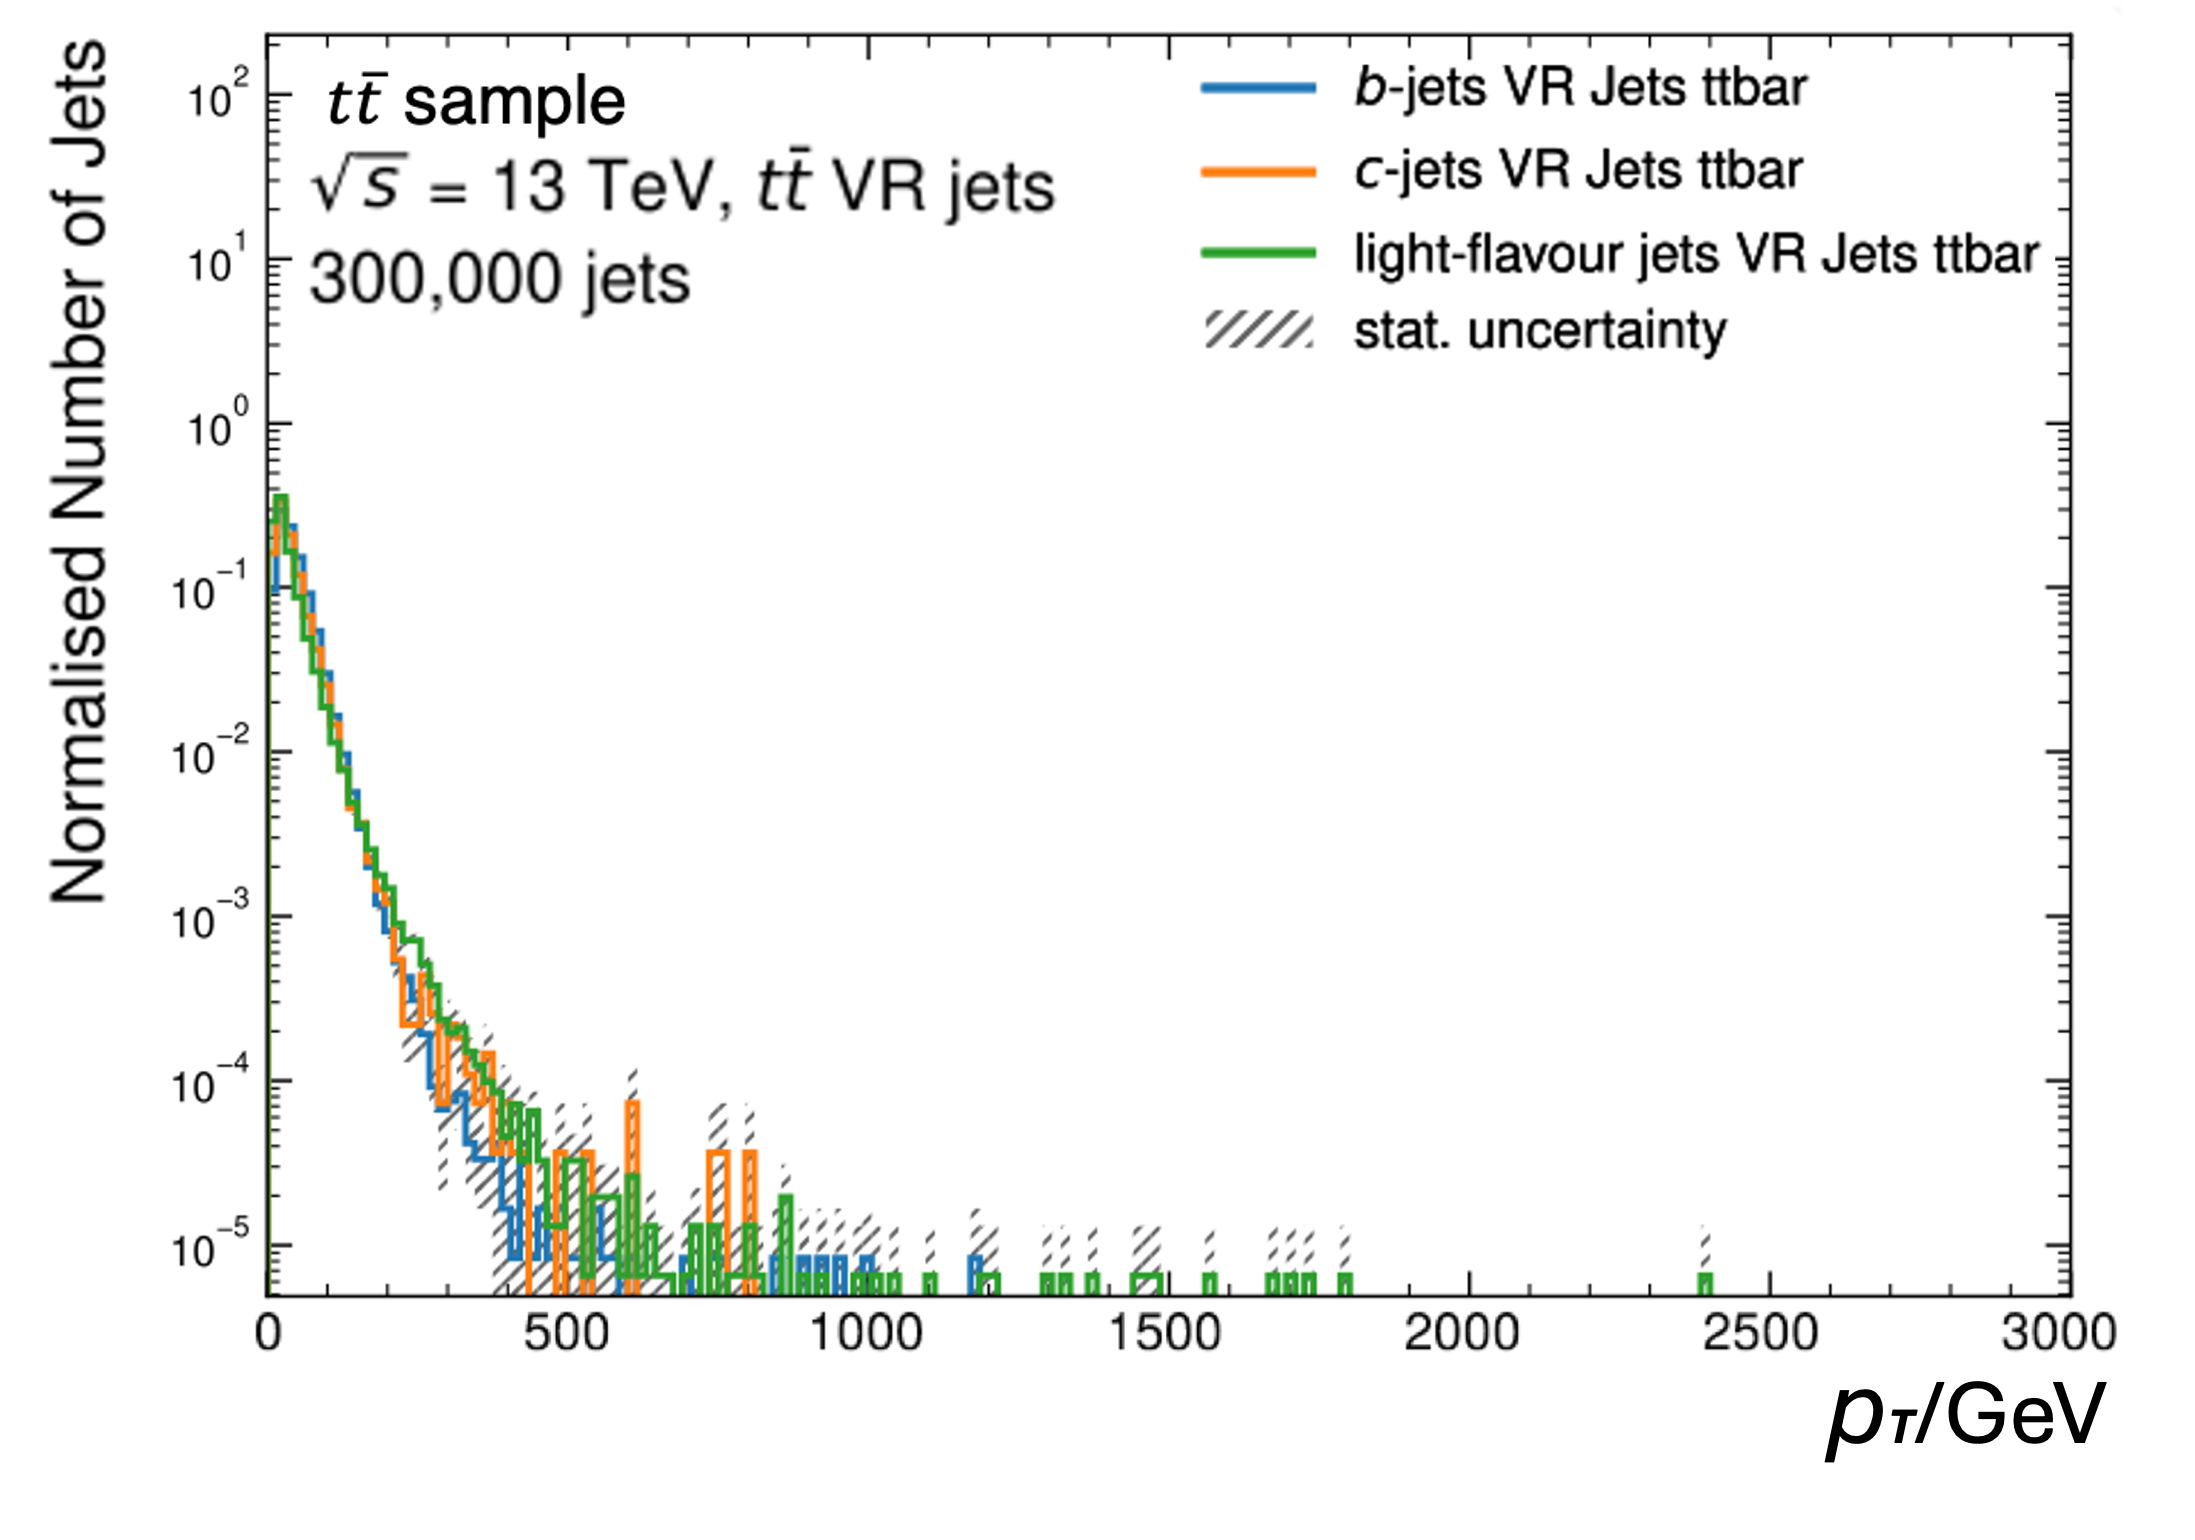
\includegraphics[width=0.48\textwidth]{Images/FTAG/VRDips/JetDist/ttpt.png}
      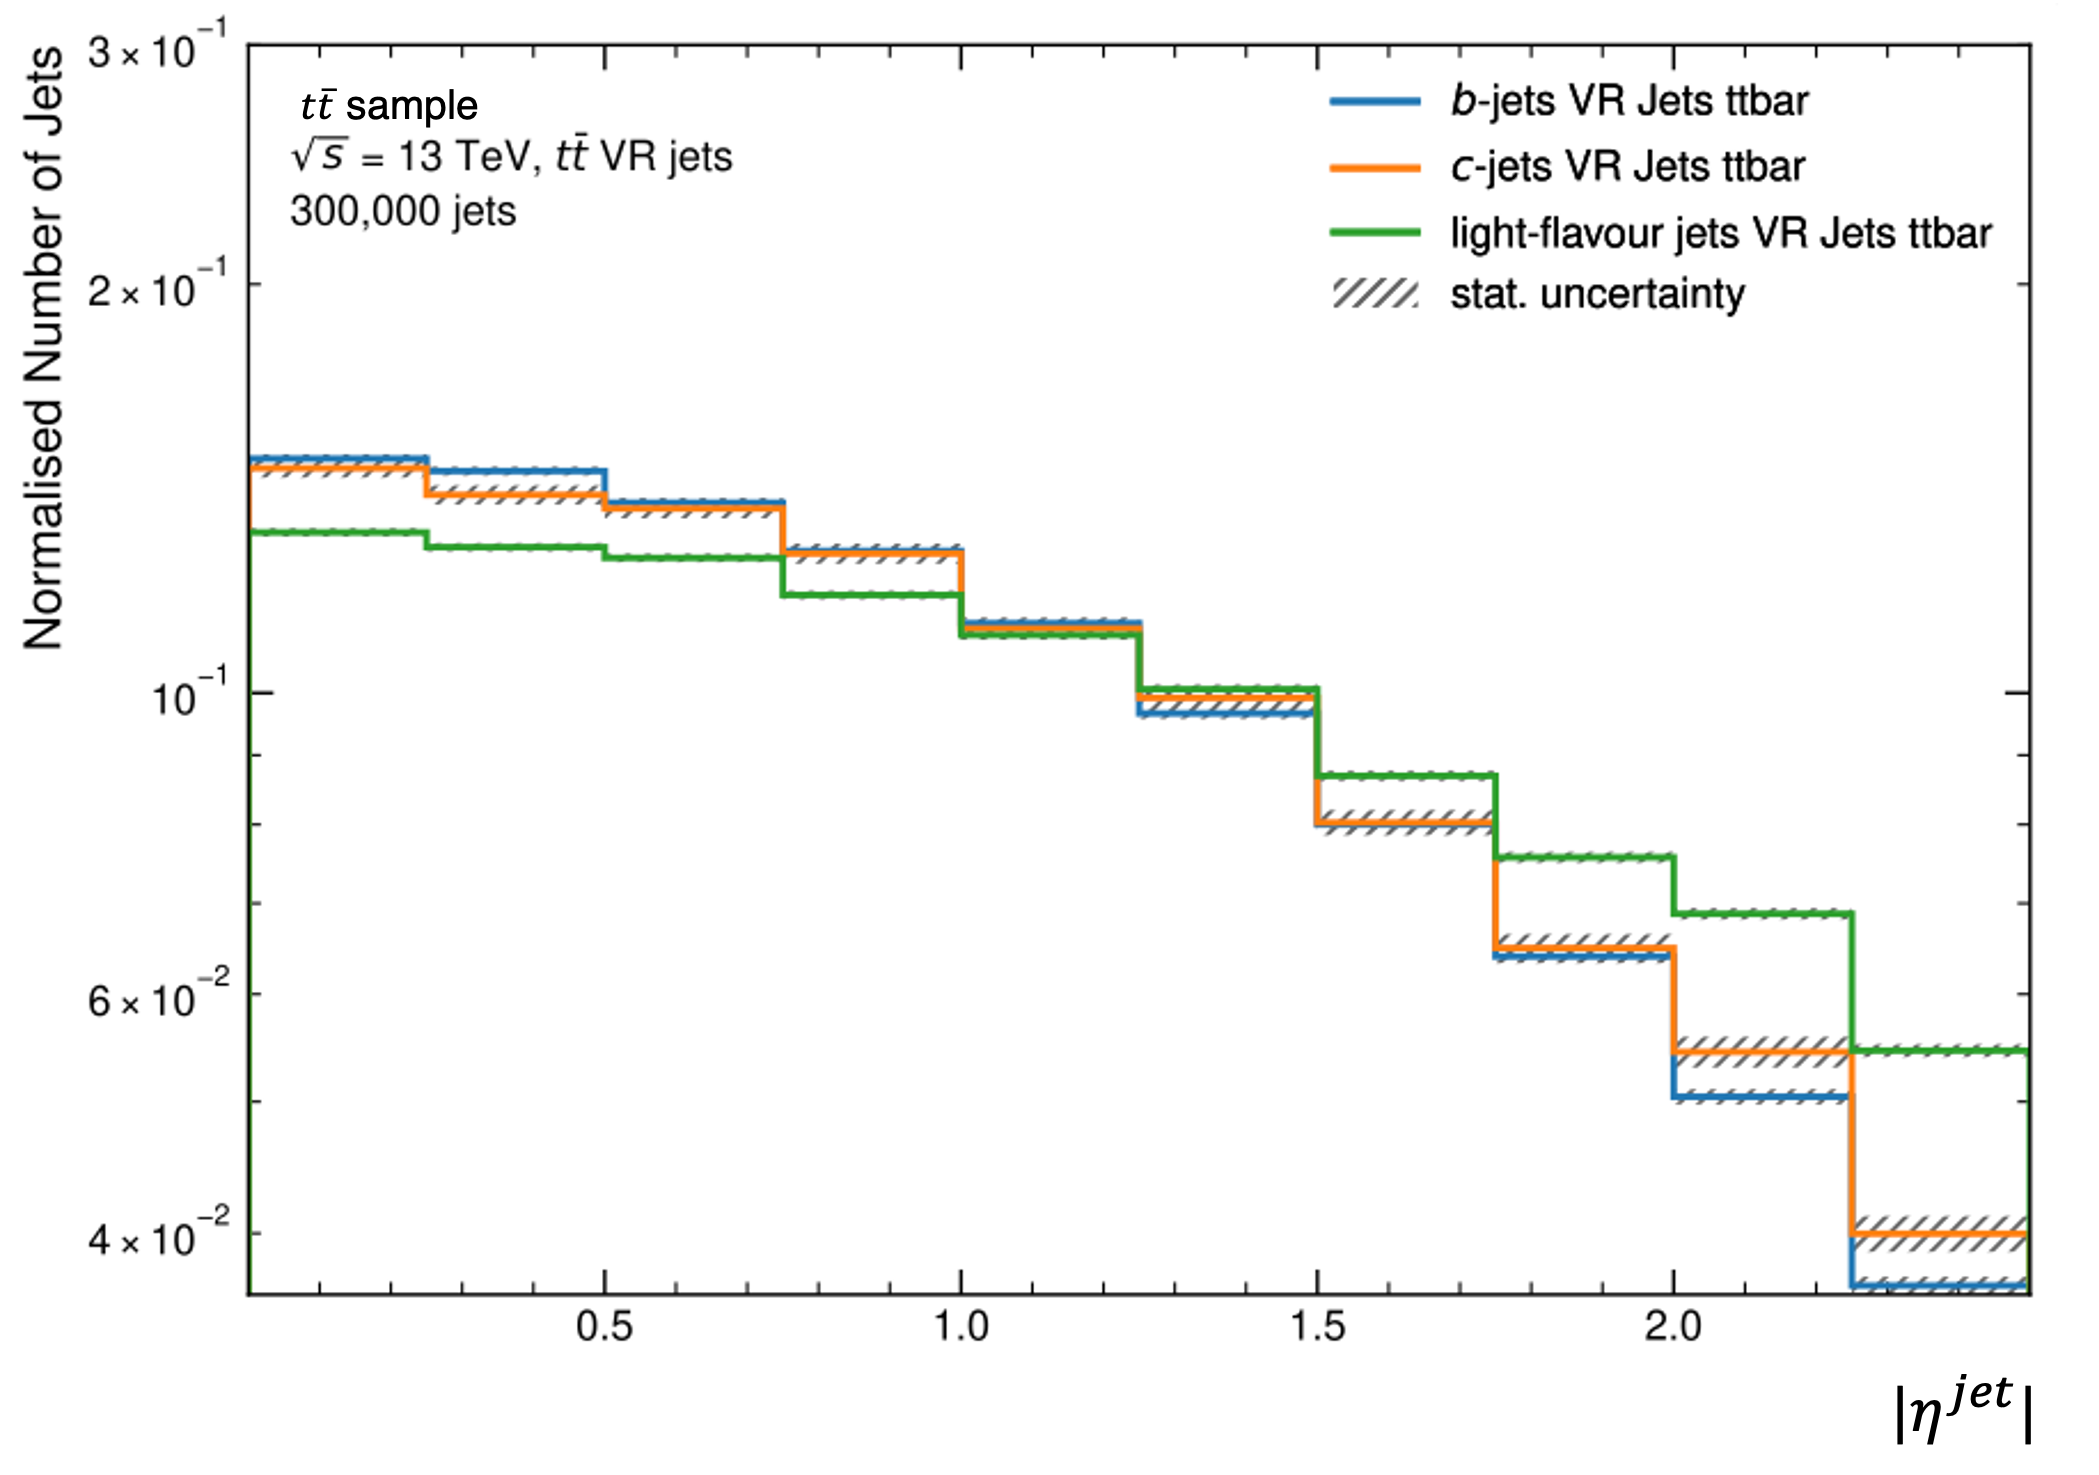
\includegraphics[width=0.48\textwidth]{Images/FTAG/VRDips/JetDist/tteta.png}
      \caption{$t\bar{t}$ sample.} 
      \label{fig:vrjetdistt}
  \end{subfigure}\\
  \begin{subfigure}[b]{0.98\textwidth}
      \centering
      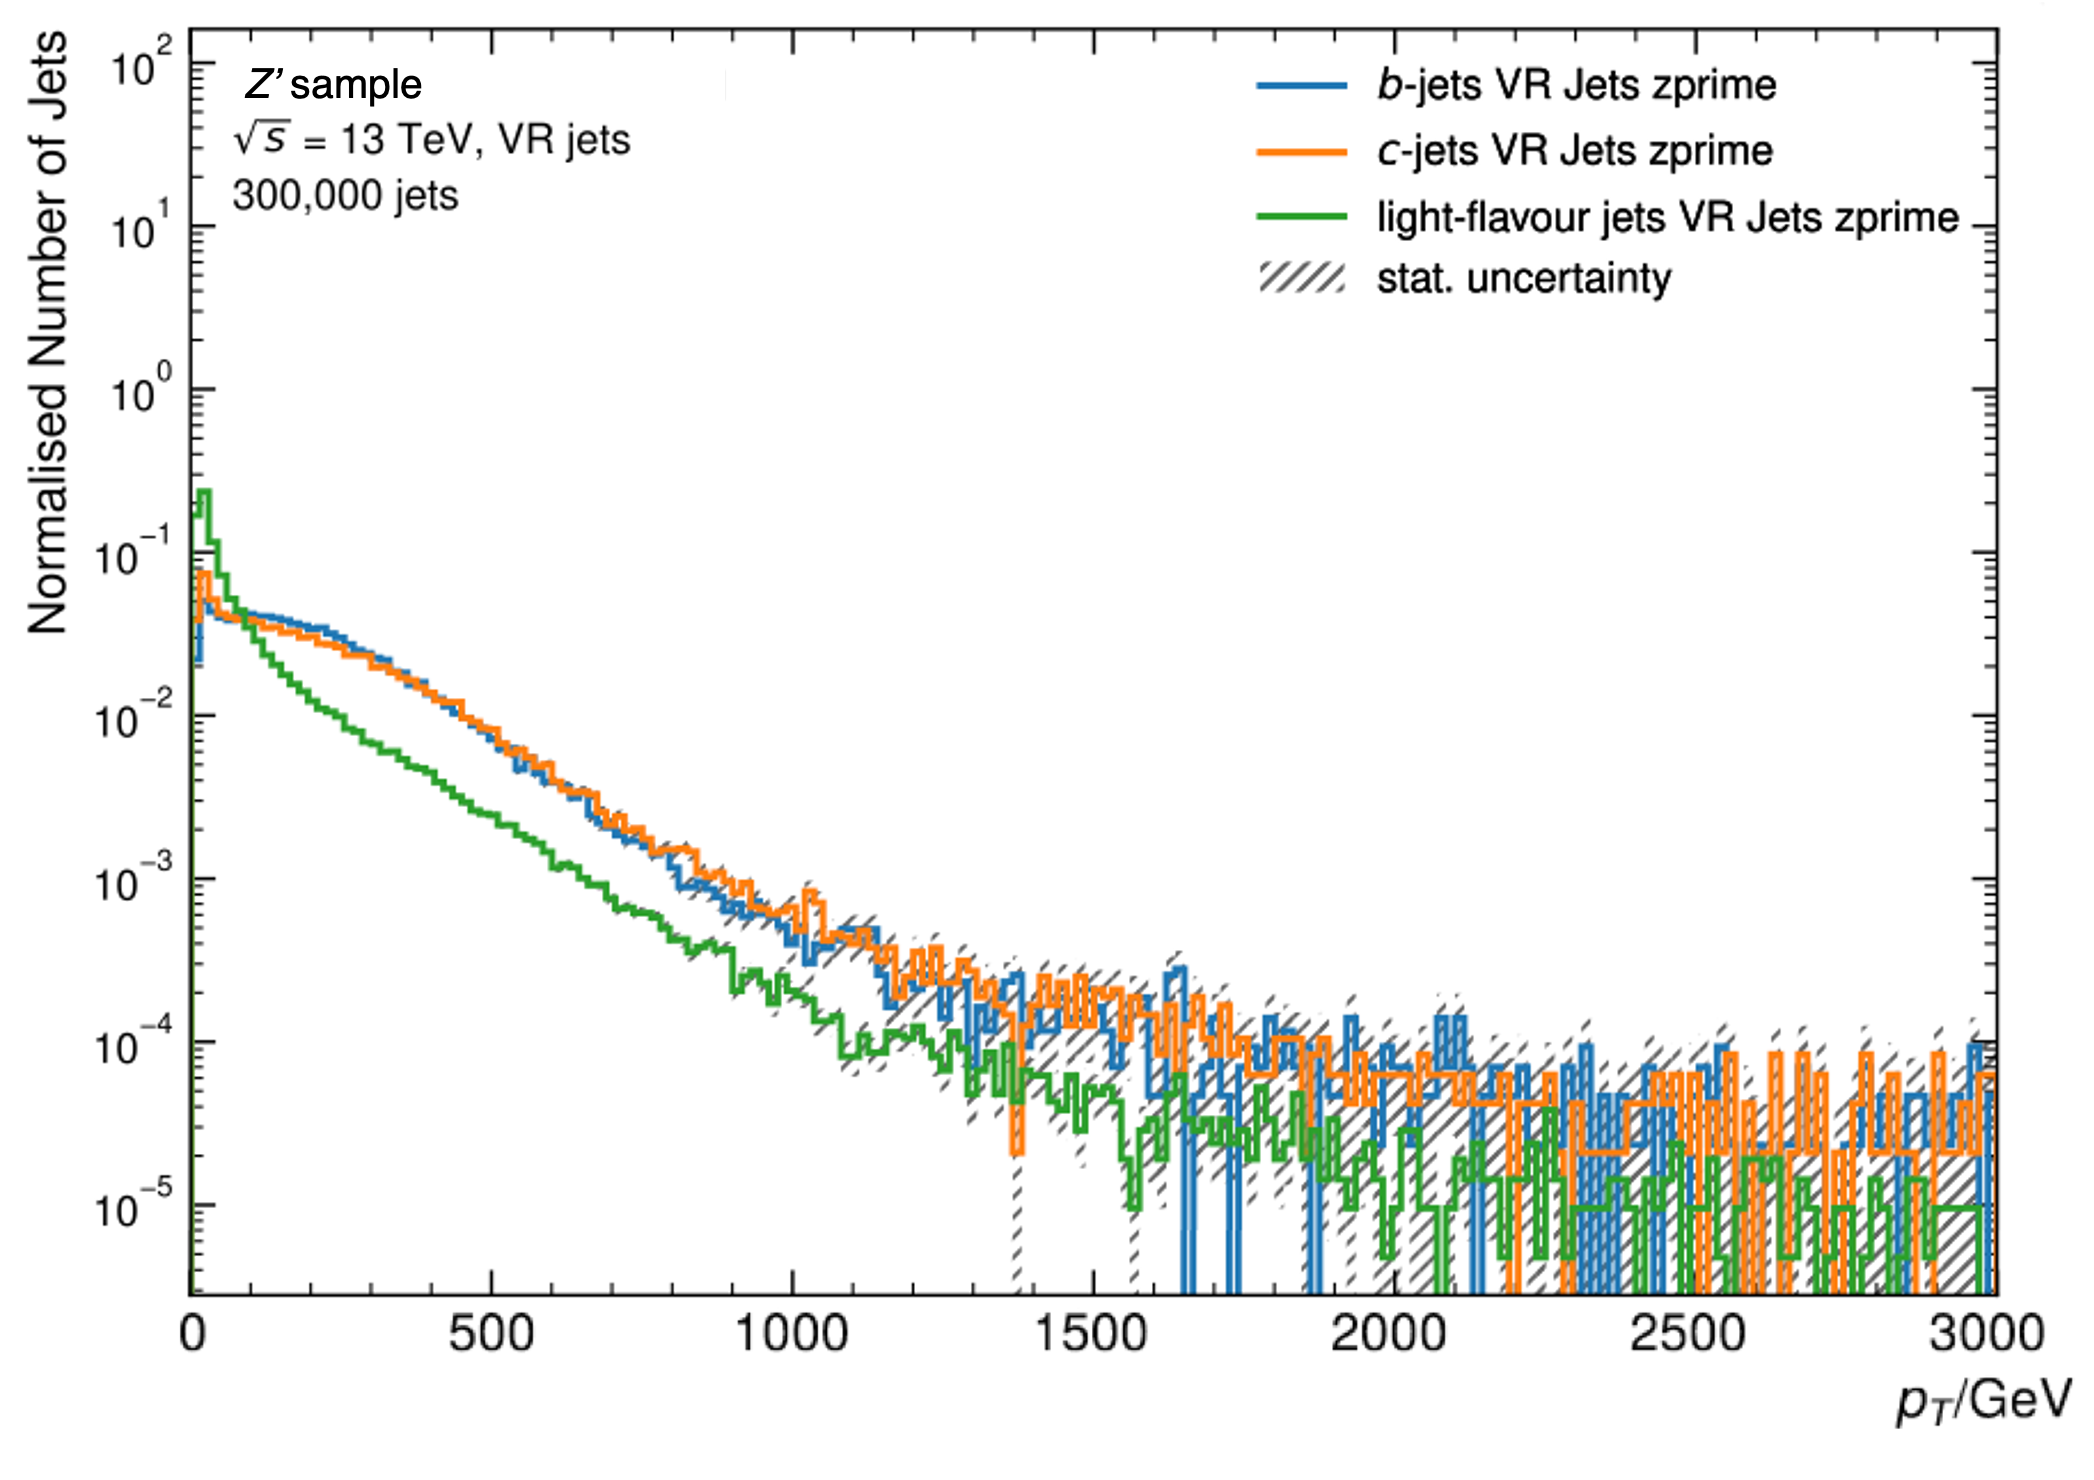
\includegraphics[width=0.48\textwidth]{Images/FTAG/VRDips/JetDist/zppt.png}
      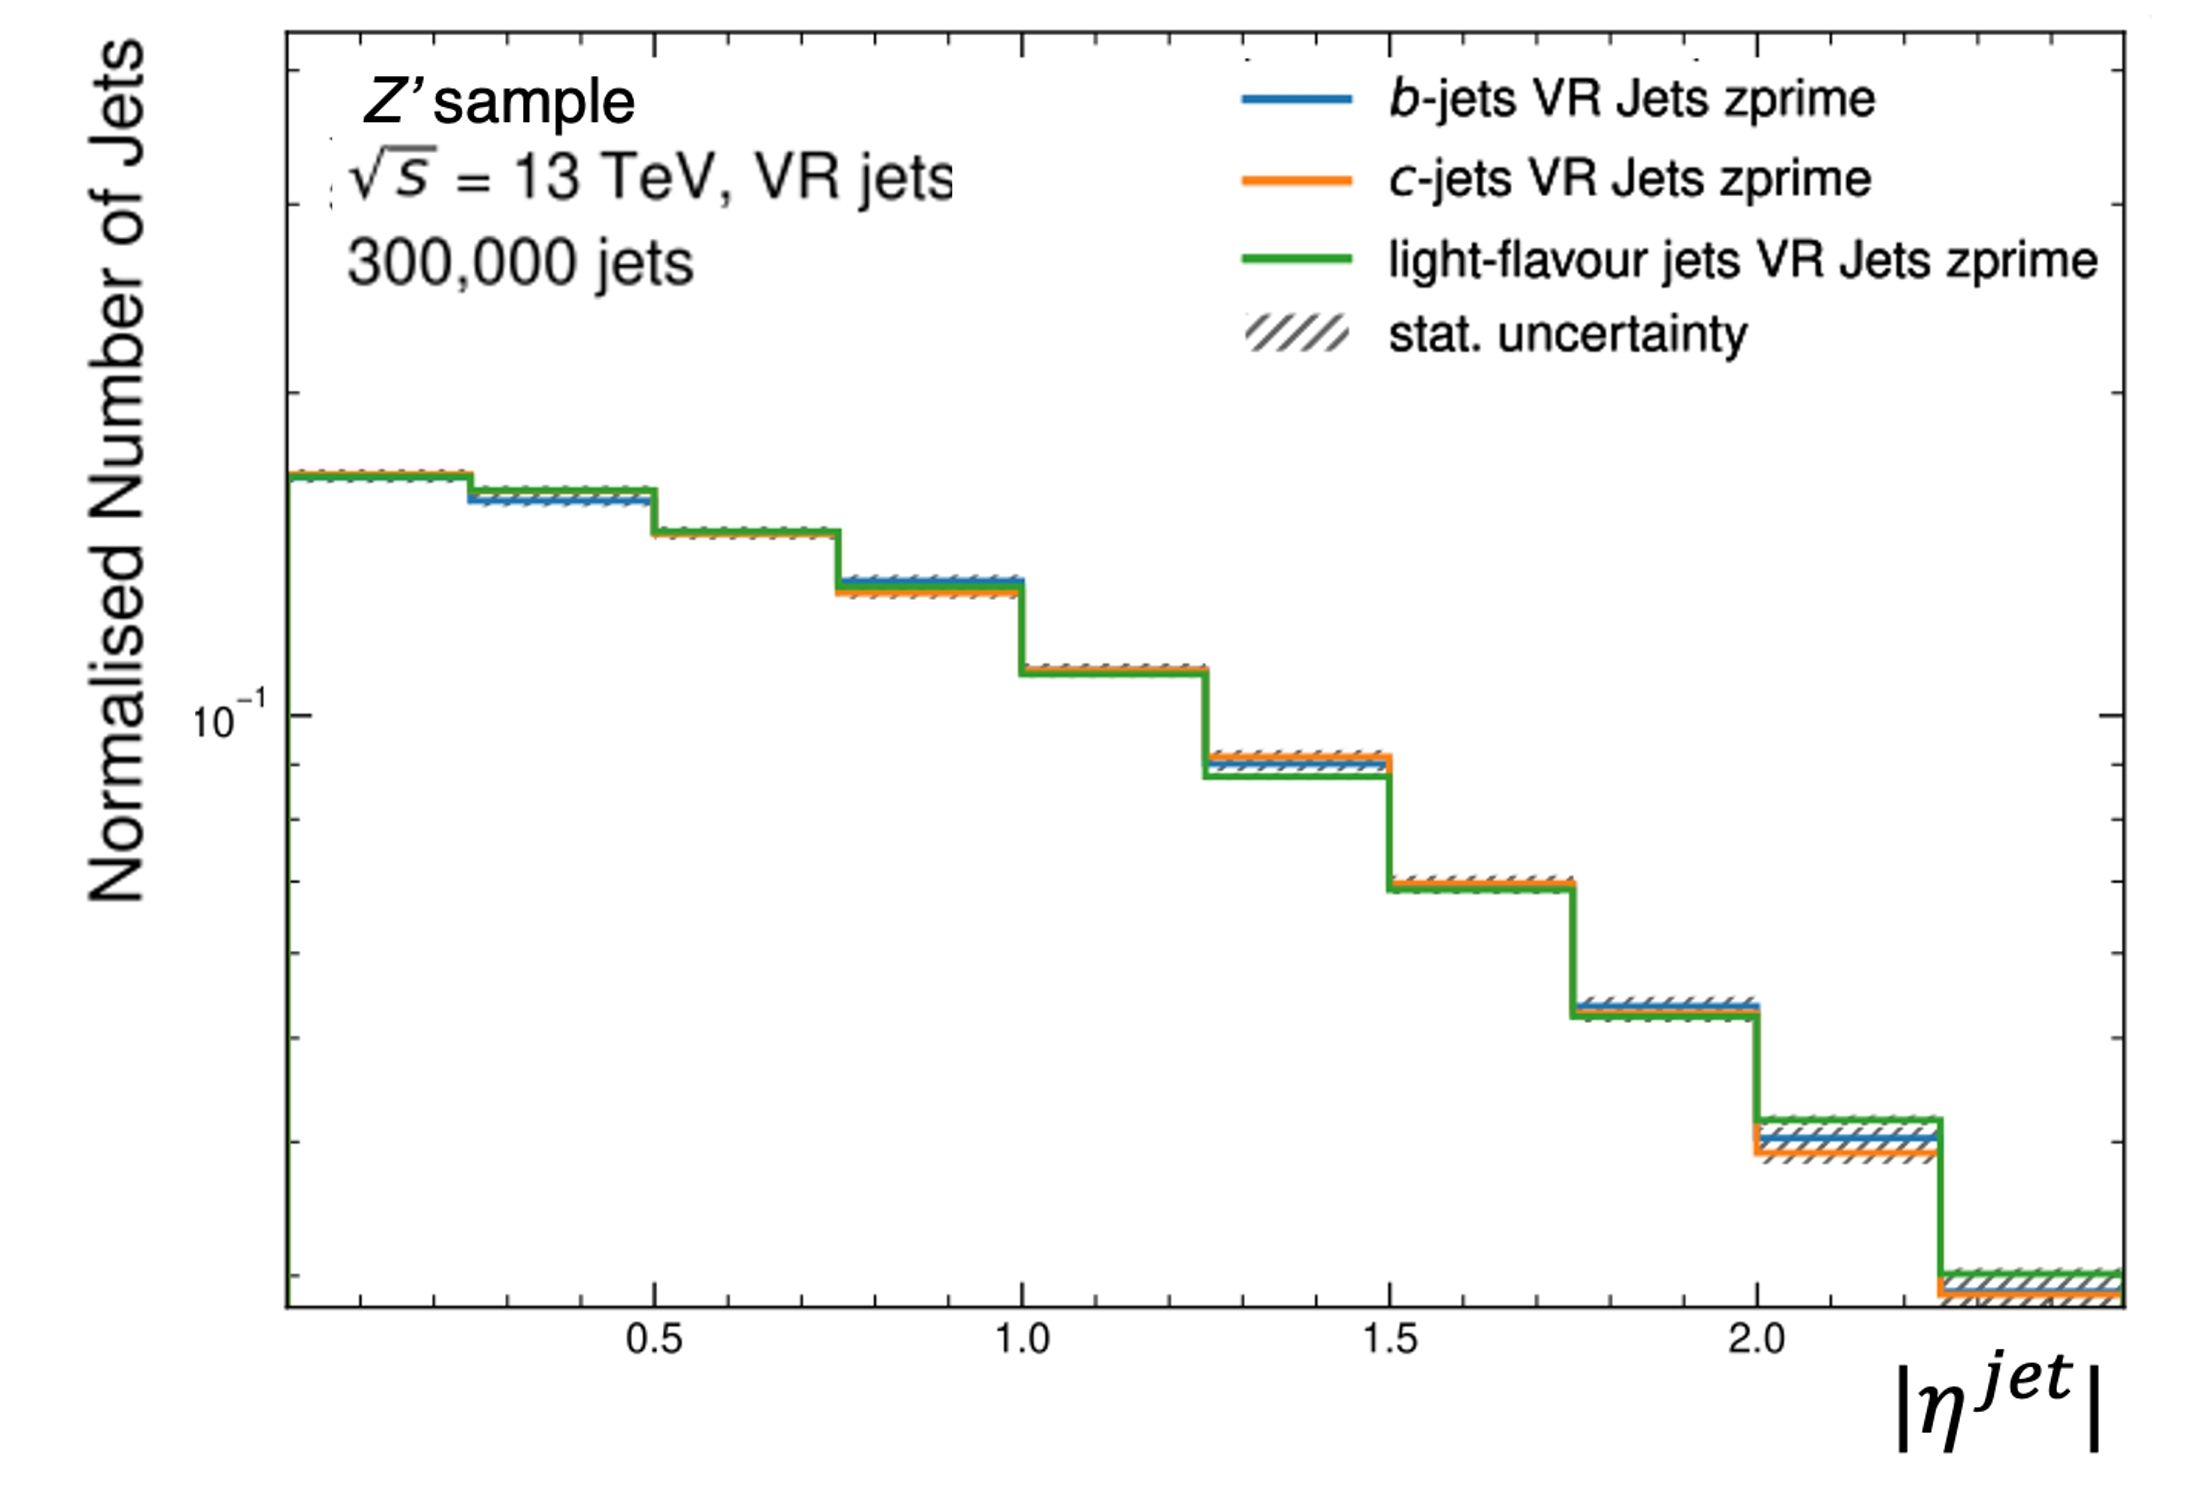
\includegraphics[width=0.48\textwidth]{Images/FTAG/VRDips/JetDist/zpeta.png}
      \caption{$Z'$ sample.} 
      \label{fig:vrjetdiszp}
  \end{subfigure}\\
  \begin{subfigure}[b]{0.98\textwidth}
      \centering
      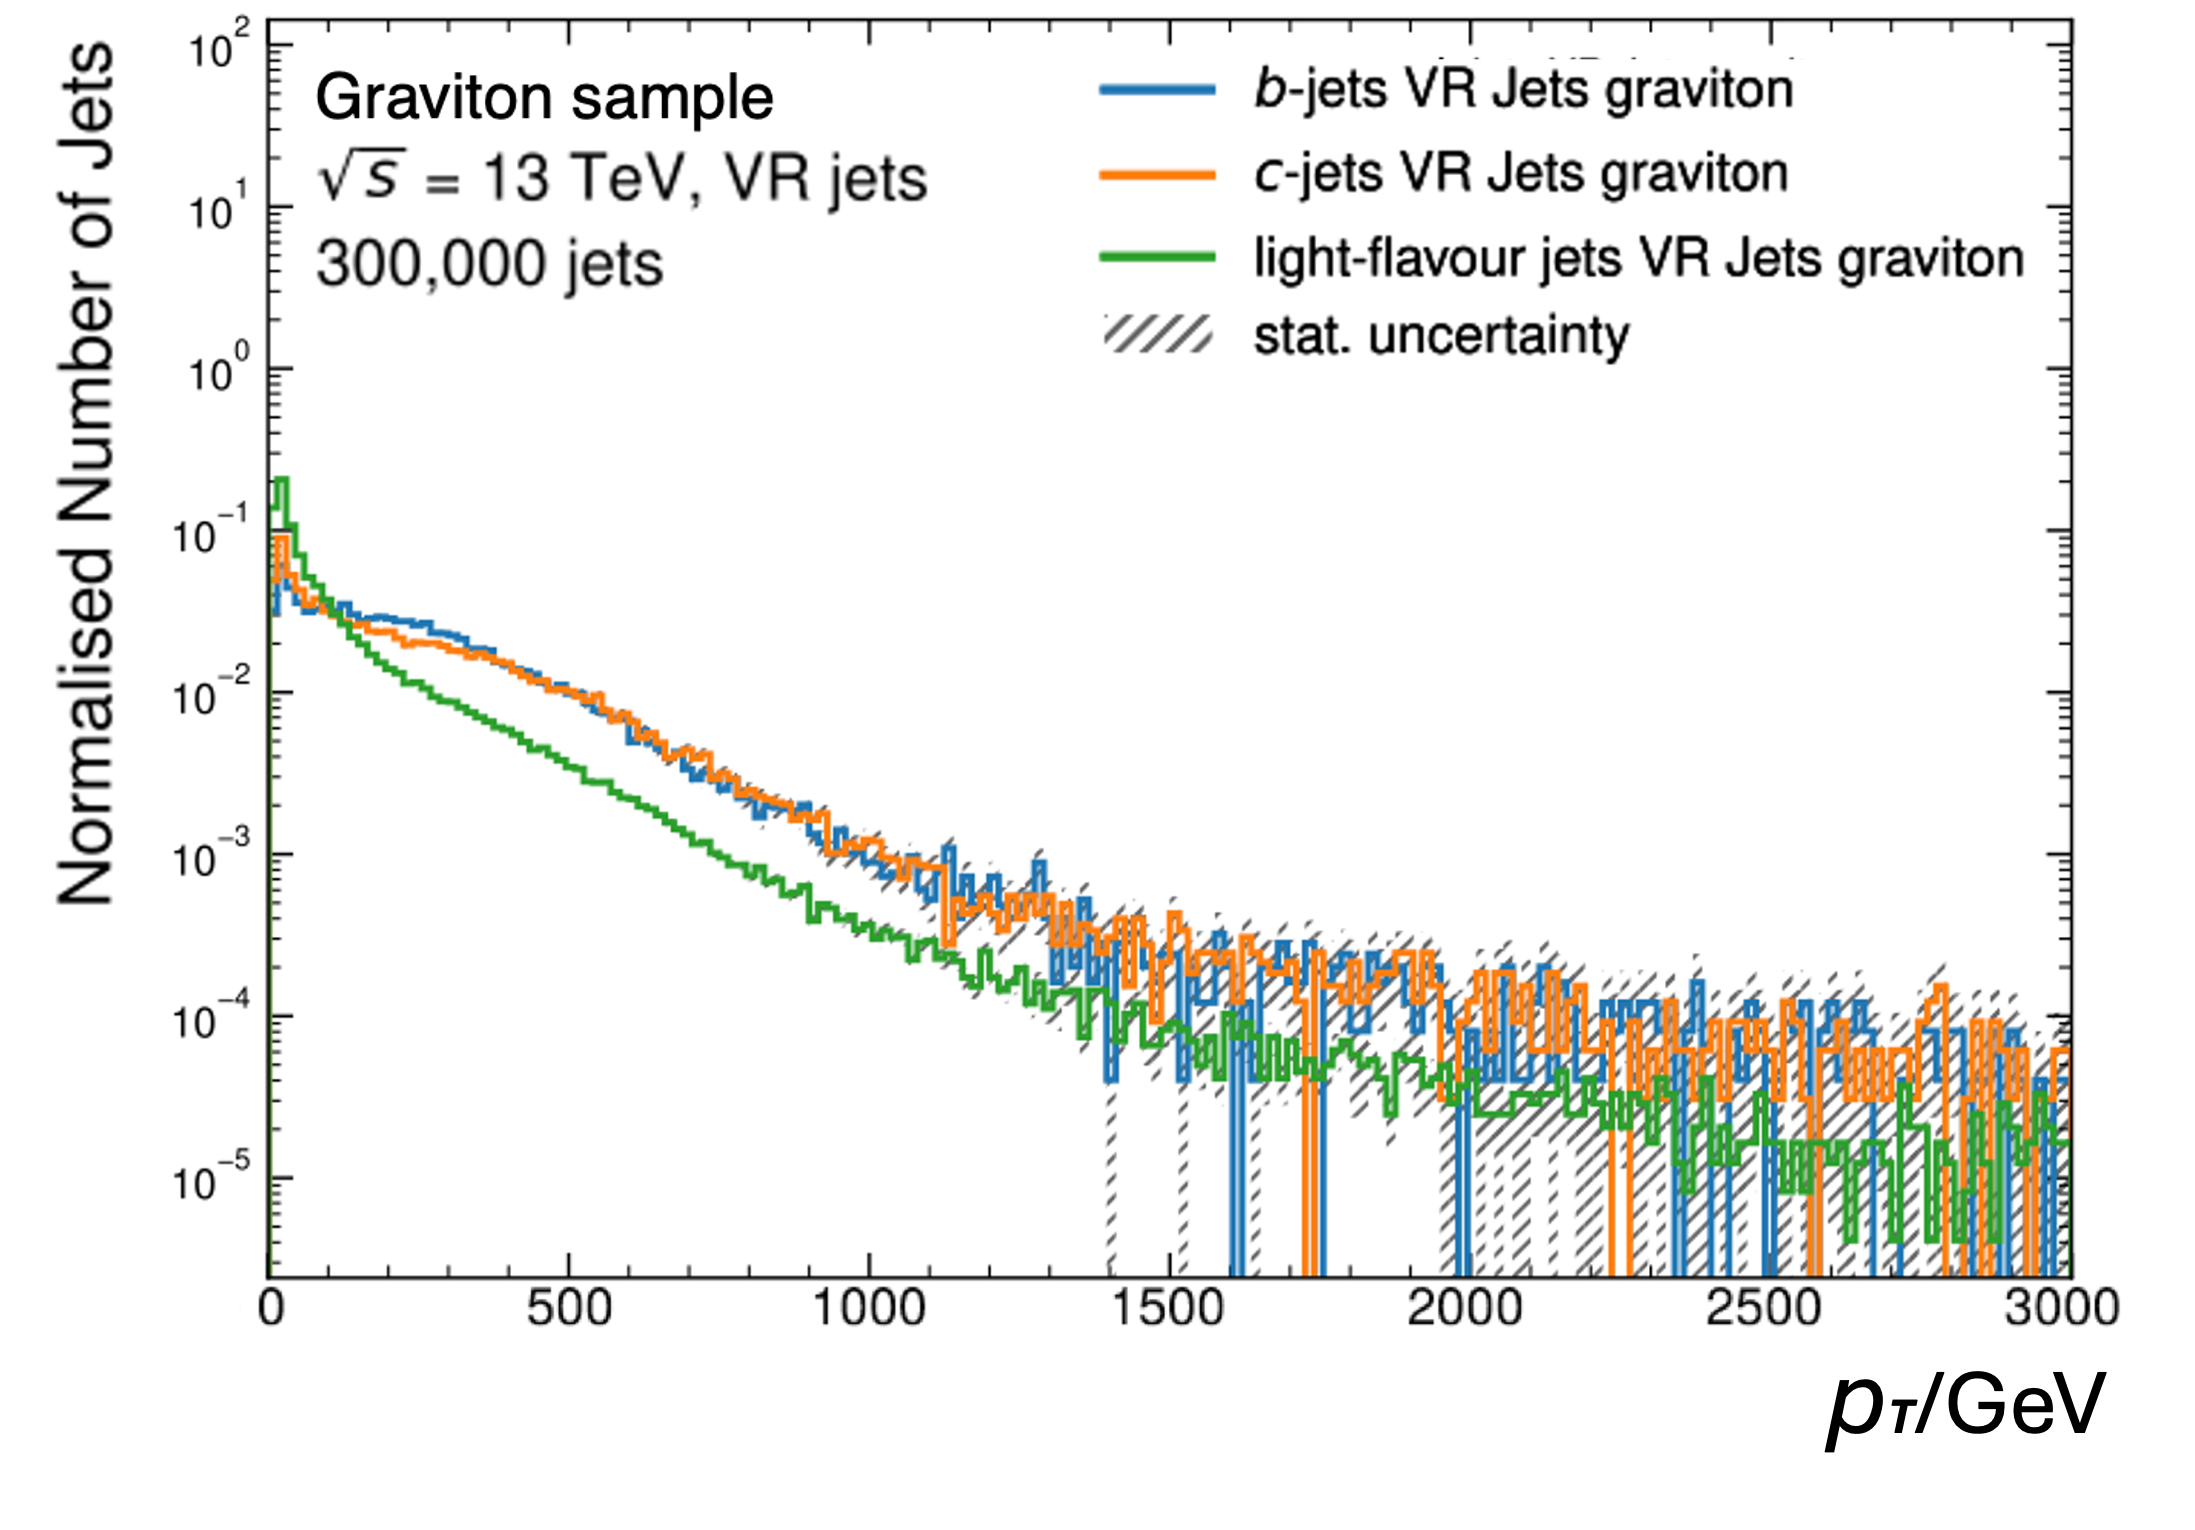
\includegraphics[width=0.48\textwidth]{Images/FTAG/VRDips/JetDist/grpt.png}
      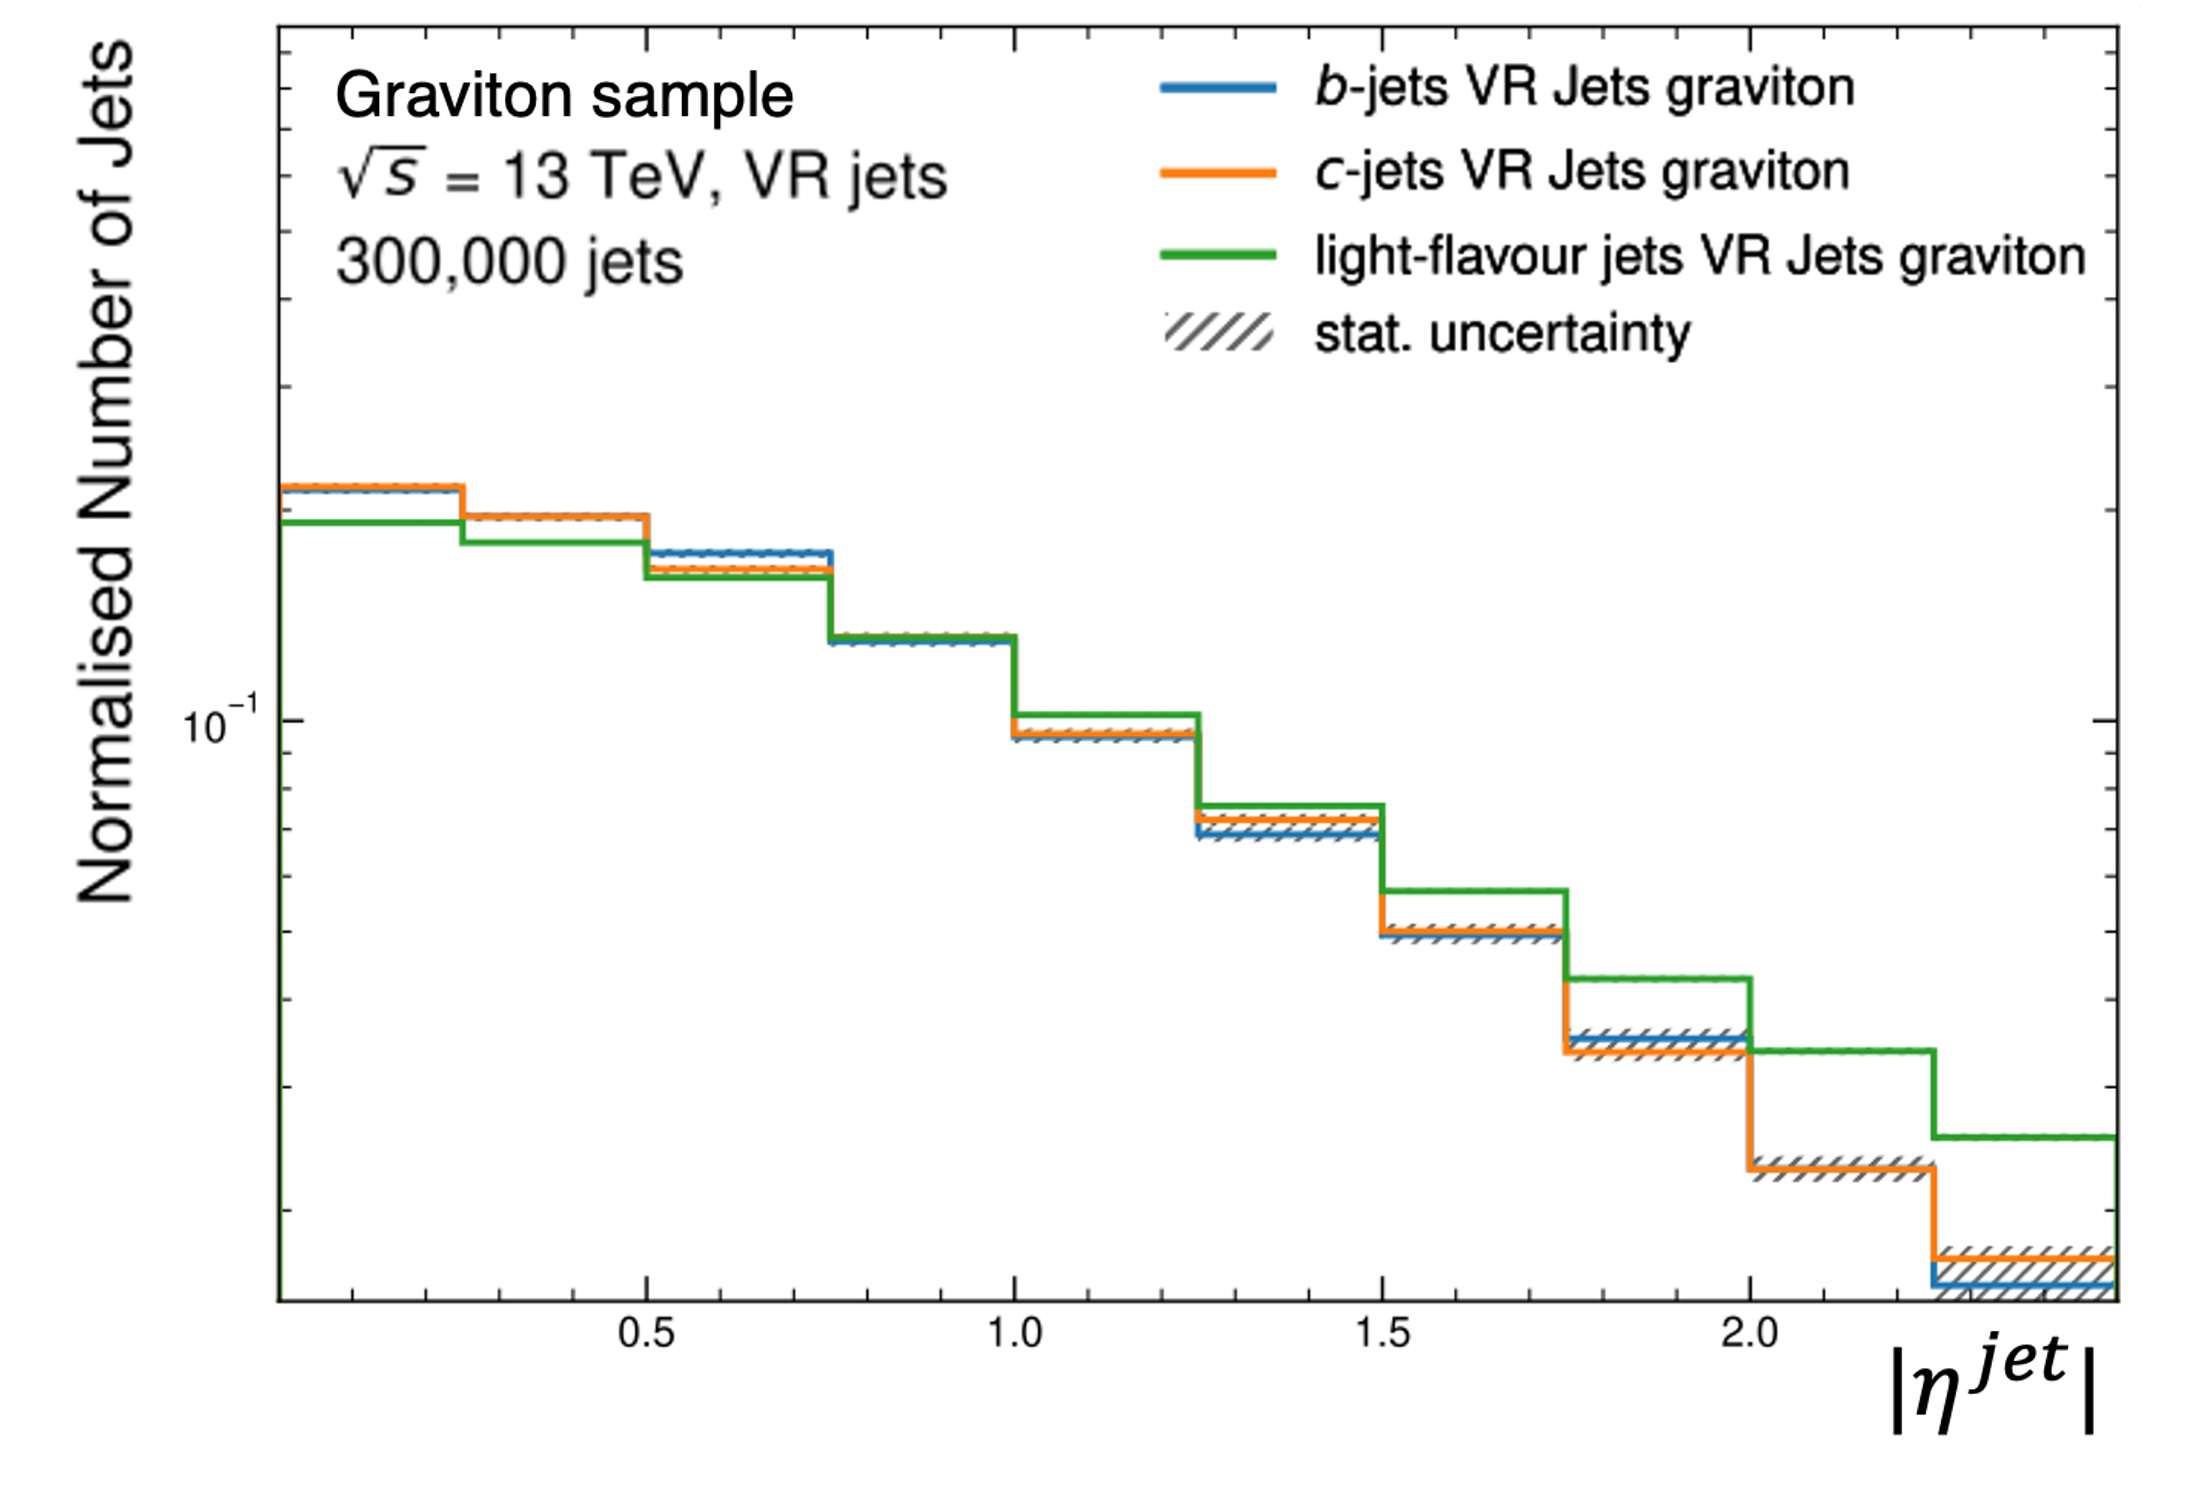
\includegraphics[width=0.48\textwidth]{Images/FTAG/VRDips/JetDist/greta.png}
      \caption{Graviton sample.} 
      \label{fig:vrjetdisgr}
  \end{subfigure}
  \caption{Distributions for the \gls{vr}-jet training of jets $p_T$ (left) and $|\eta|$ (right) for the hybrid combined process (top row) made from the three bottom processes, in the order $t\bar{t}$, $Z'$, and the graviton.}
  \label{fig:vrjetdist}
\end{figure} 
 
The optimised \gls{dips} model with 62,167 learnable parameters from the previous section was trained for 200 epochs on 4 Quadro RTX 8000 \gls{gpu}. The learning rate started at 0.001 and was reduced by a factor 0.8 on plateaus of 3 epochs, with a batch size of 15k jets, batch normalisation, and a dropout rate of 0.1 for the $F$ network. Training proved stable with no signs of overtraining. The model at the epoch giving the smallest loss on a heldout validation set of 300k jets as well as the best light- and $c$-rejections at a fixed 77\% $b$-tagging efficiency was selected for further comparison. Figure \ref{fig:dipsVRROC} shows the \gls{roc} curves for $b$- and $c$-tagging of the best \gls{dips} model on \gls{vr}-jets (blue), as well as some comparison to the \gls{dips} model trained on PFlow jets (orange) and \gls{rnnip} trained on \gls{vr}-jets from the previous software release R21 (green). 

\begin{sidewaysfigure}
  \vspace{0.5cm}
  %\hspace{0.5cm}
  \begin{subfigure}[t]{0.3\textwidth}
    \centering
    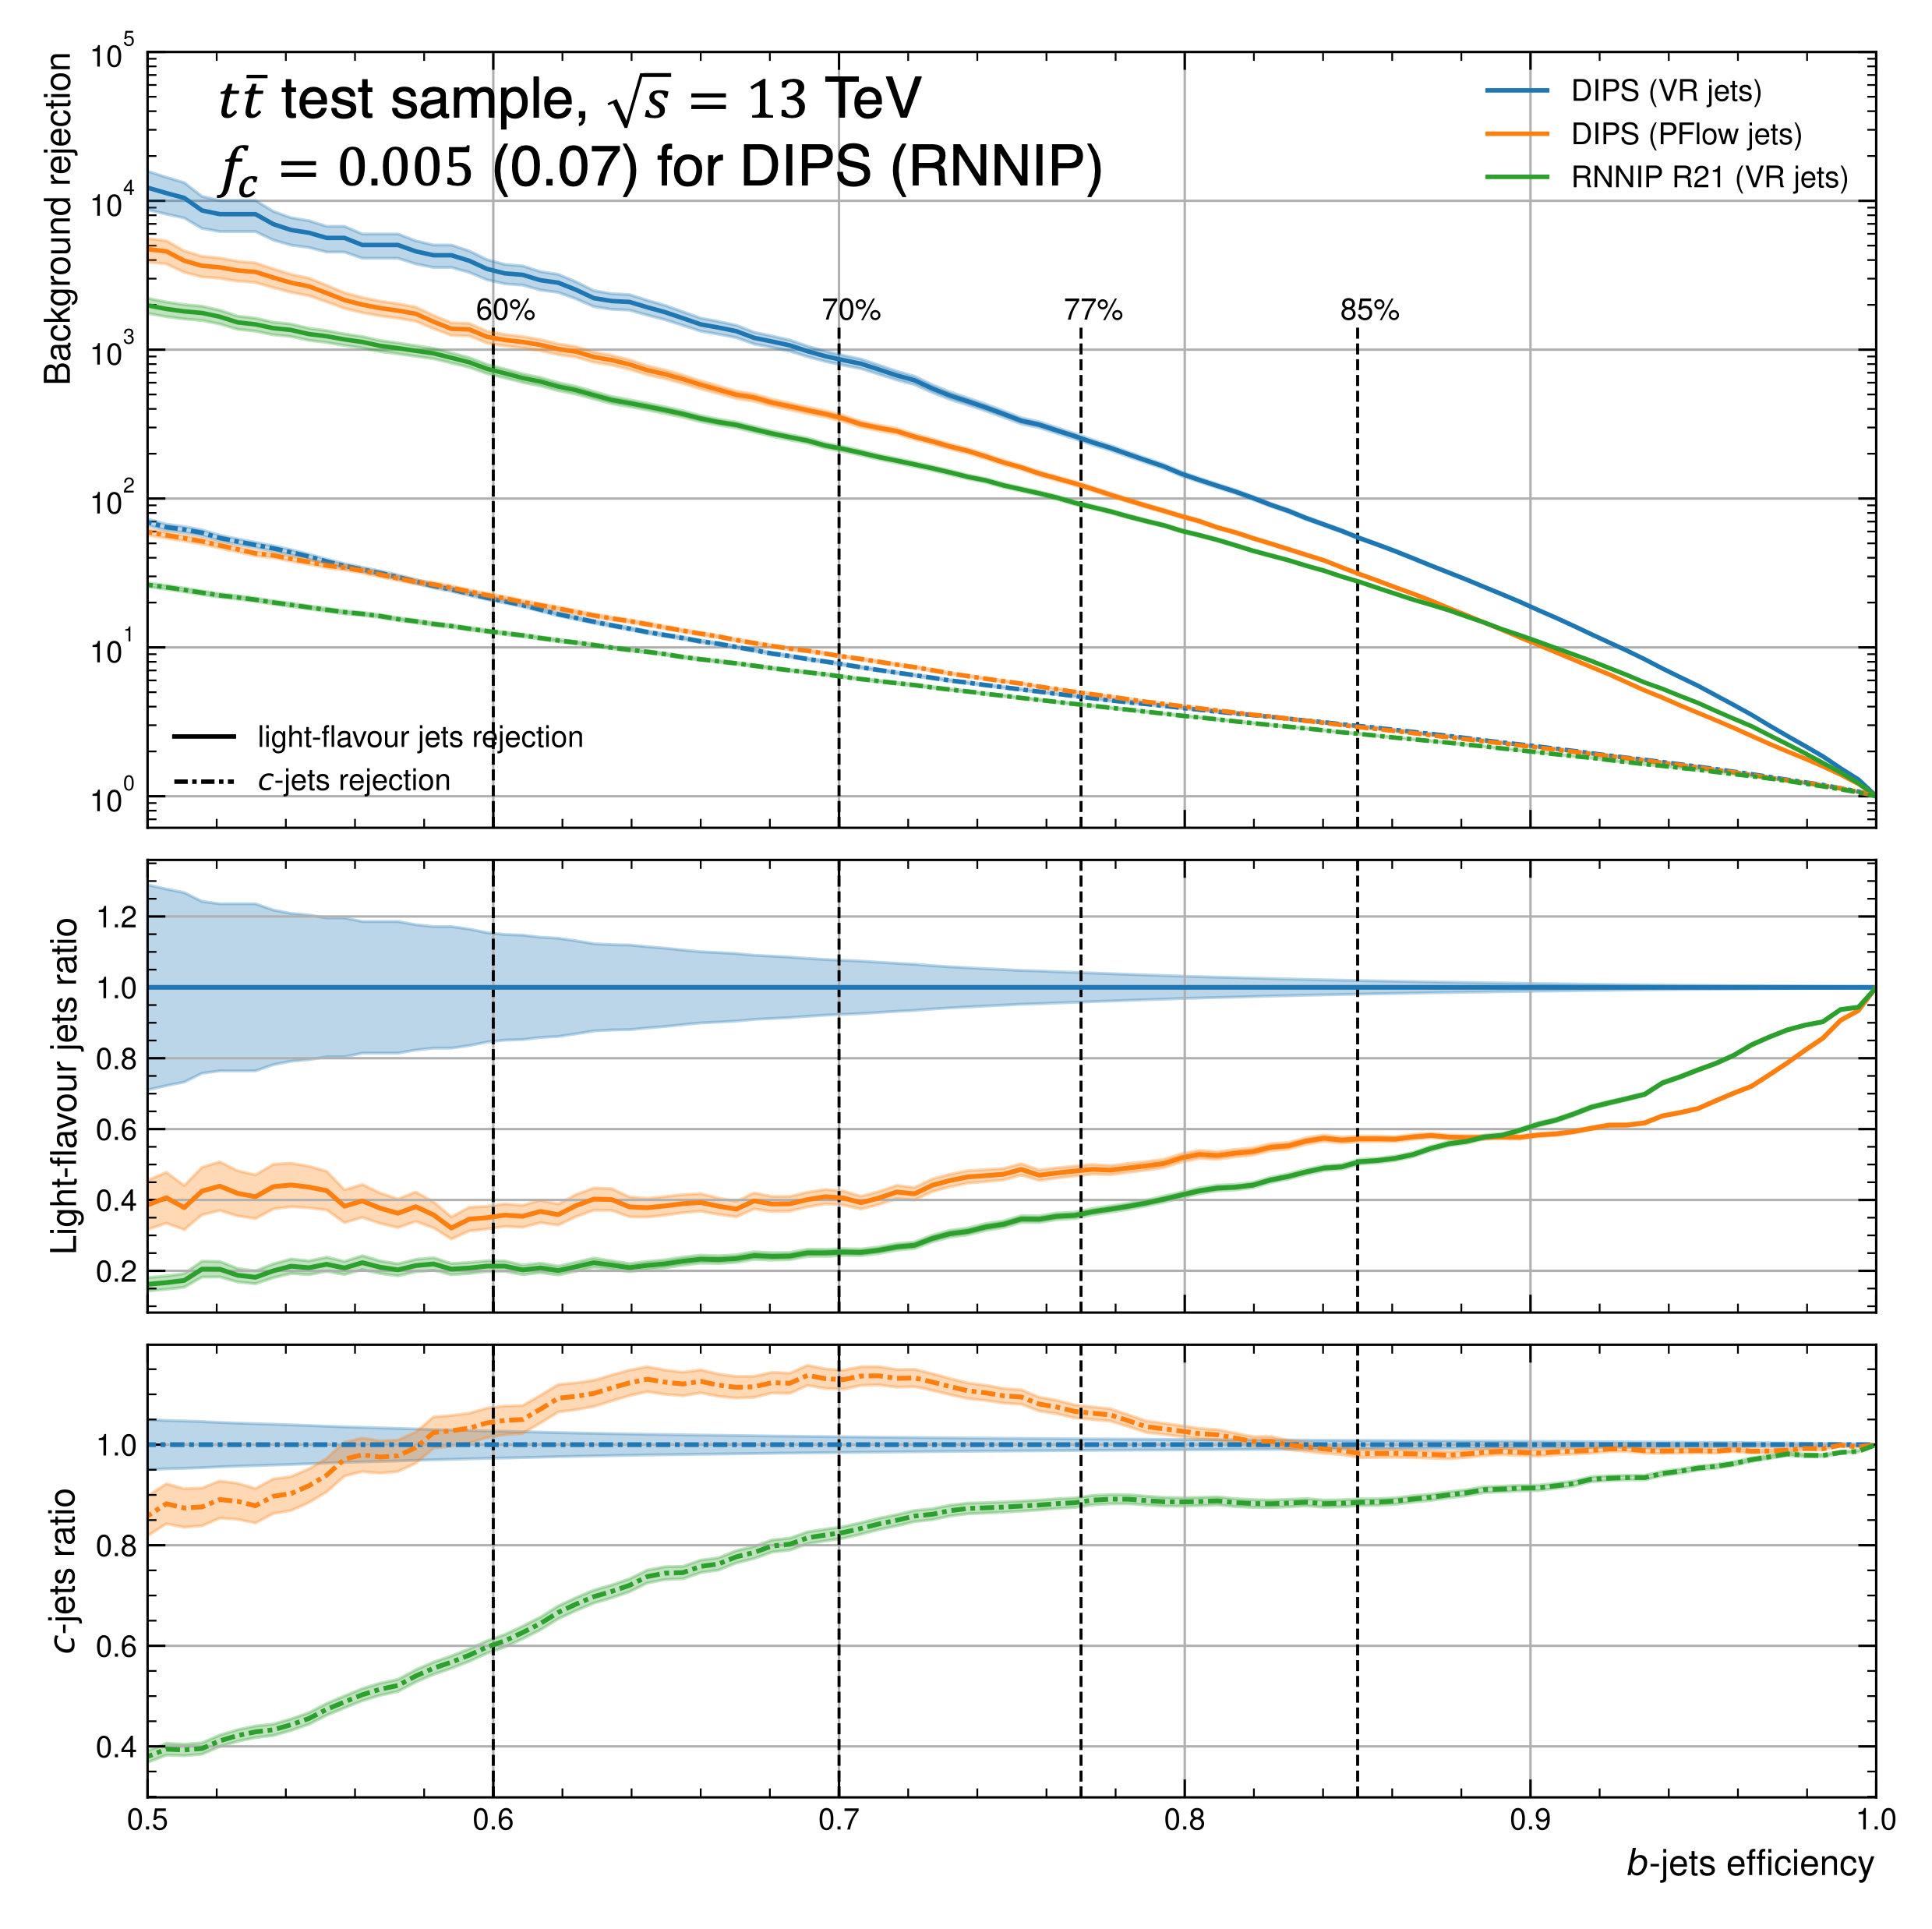
\includegraphics[scale=0.43]{Images/FTAG/VRDips/ROC/ttb.png}
    \caption{$t\bar{t}$ test sample $b$-tagging.}
    \label{fig:dipsVRROCtt}
  \end{subfigure}
  \hfill
  \begin{subfigure}[t]{0.3\textwidth}
    \centering
    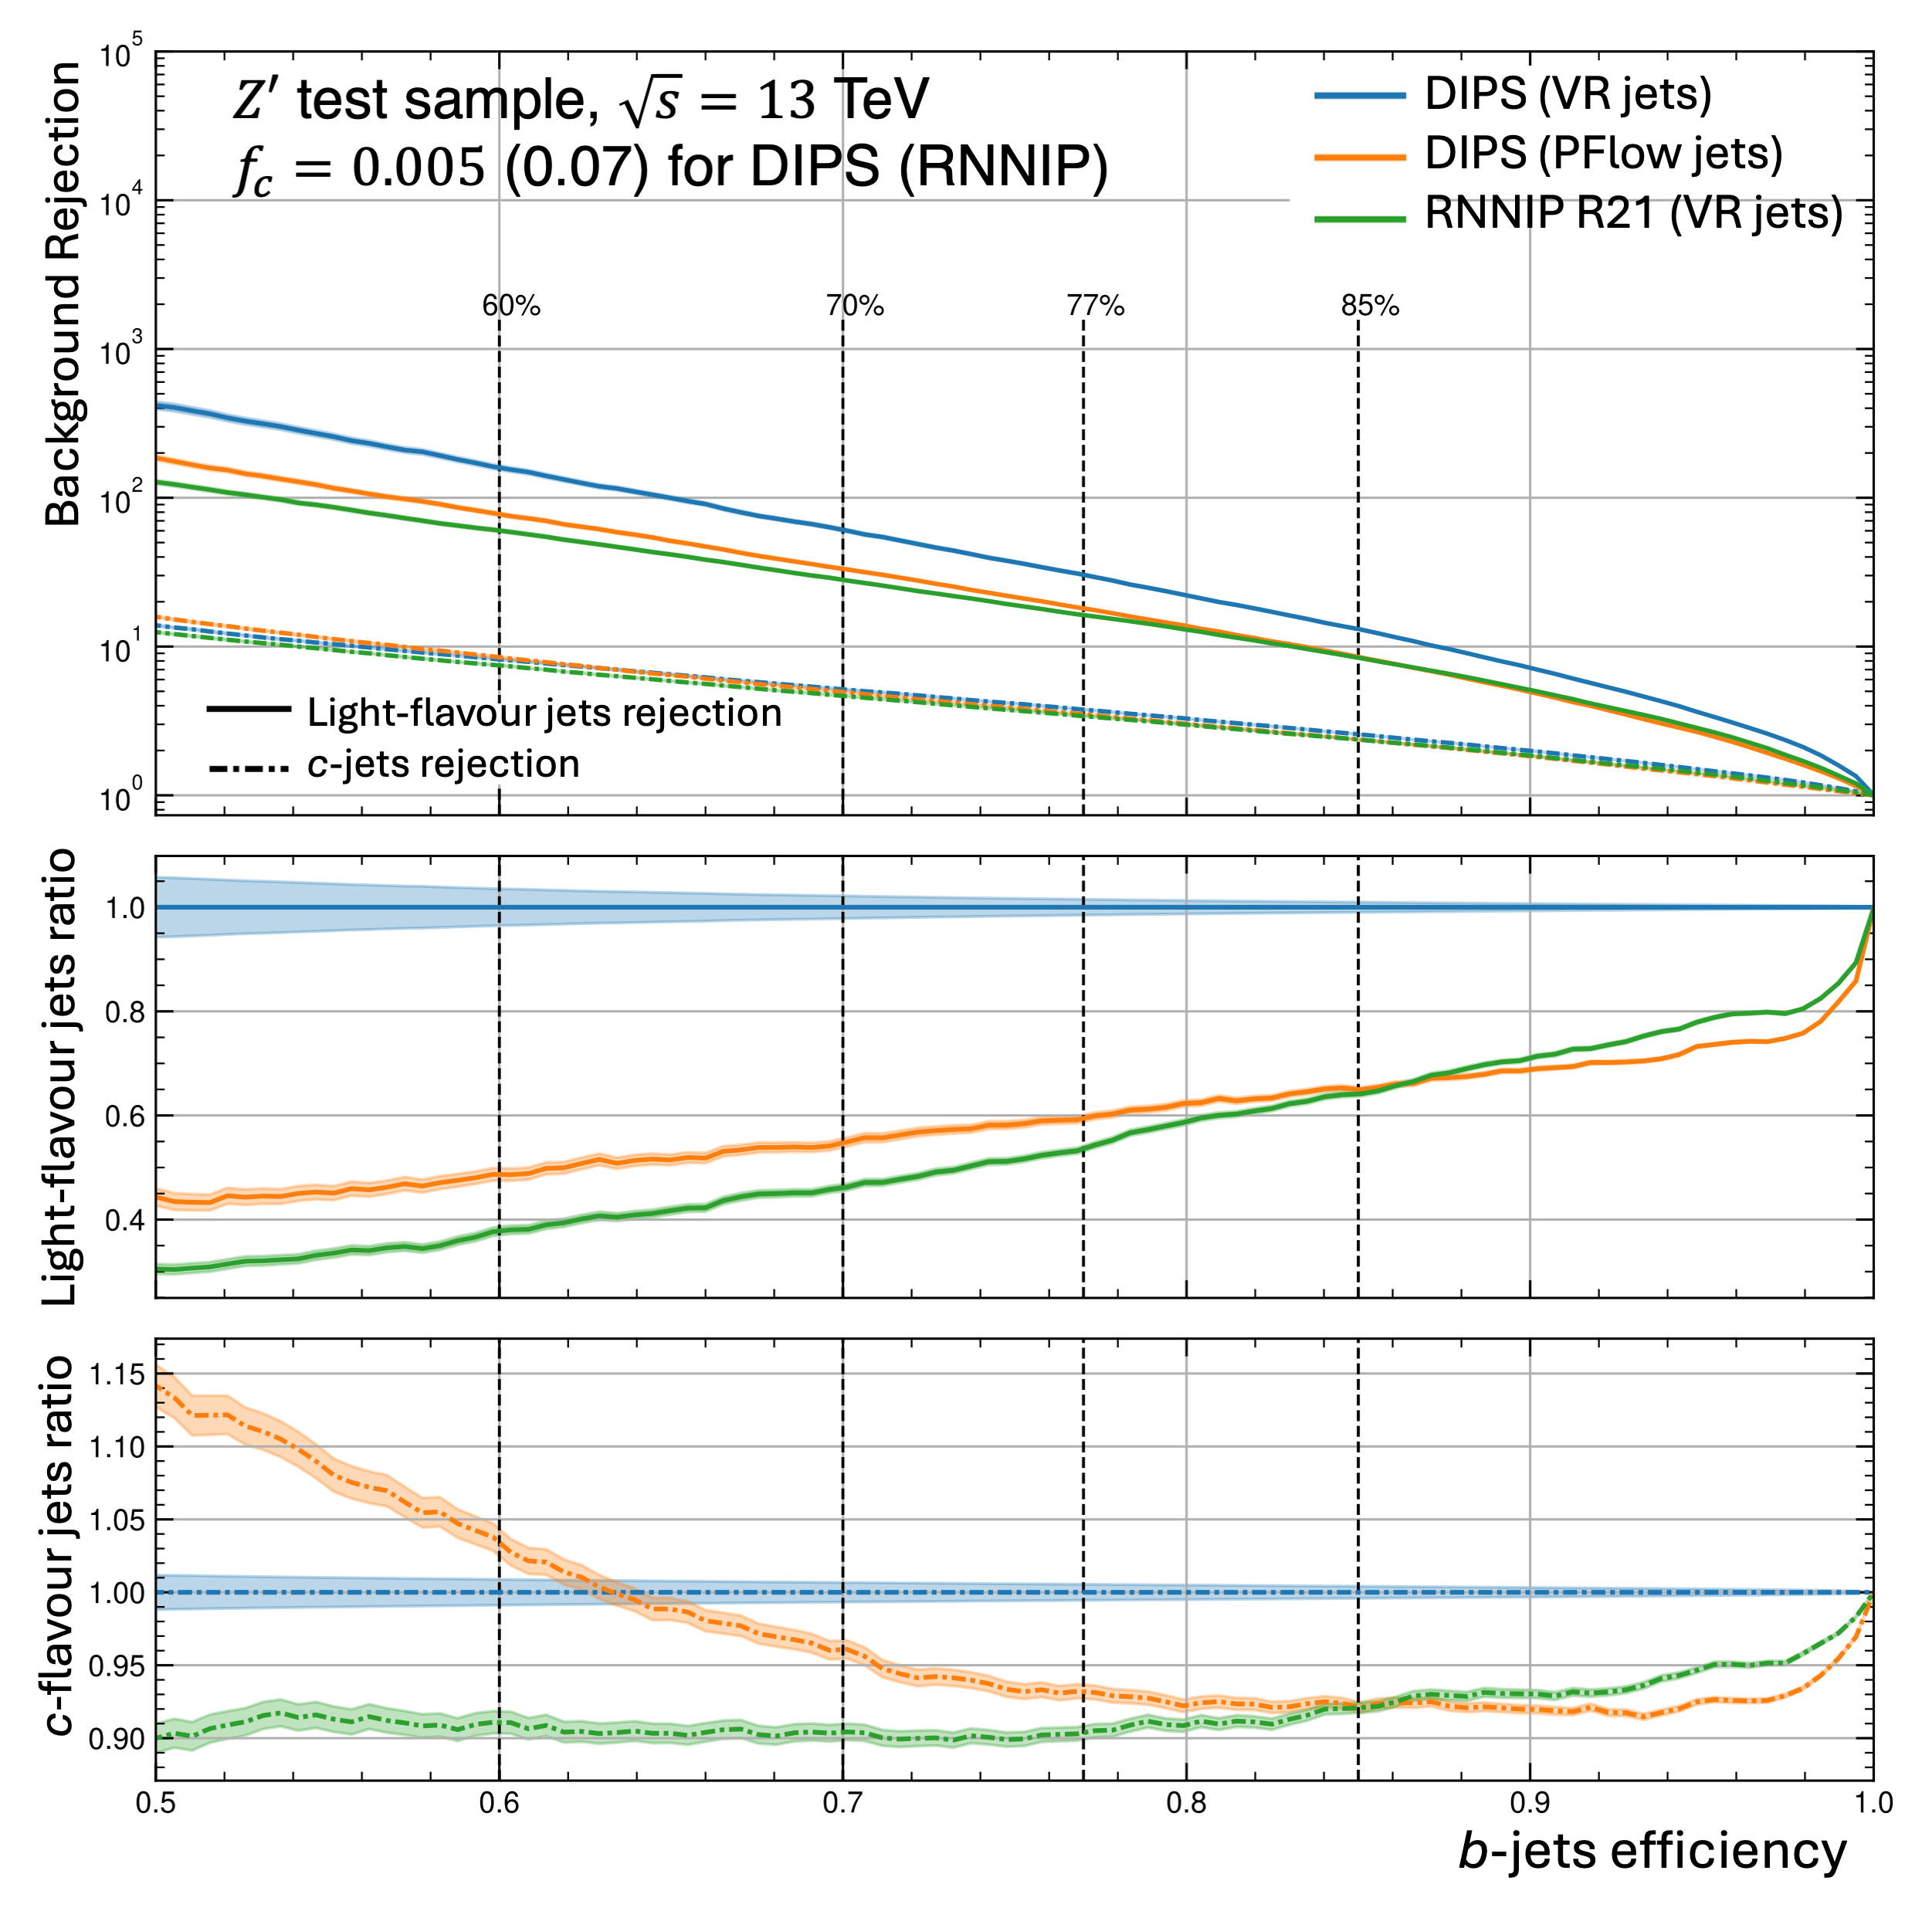
\includegraphics[scale=0.43]{Images/FTAG/VRDips/ROC/zpb.png}
    \caption{$Z'$ test sample $b$-tagging.}
    \label{fig:dipsVRROCzp}
  \end{subfigure}
  \hfill
  \begin{subfigure}[t]{0.3\textwidth}
    \centering
    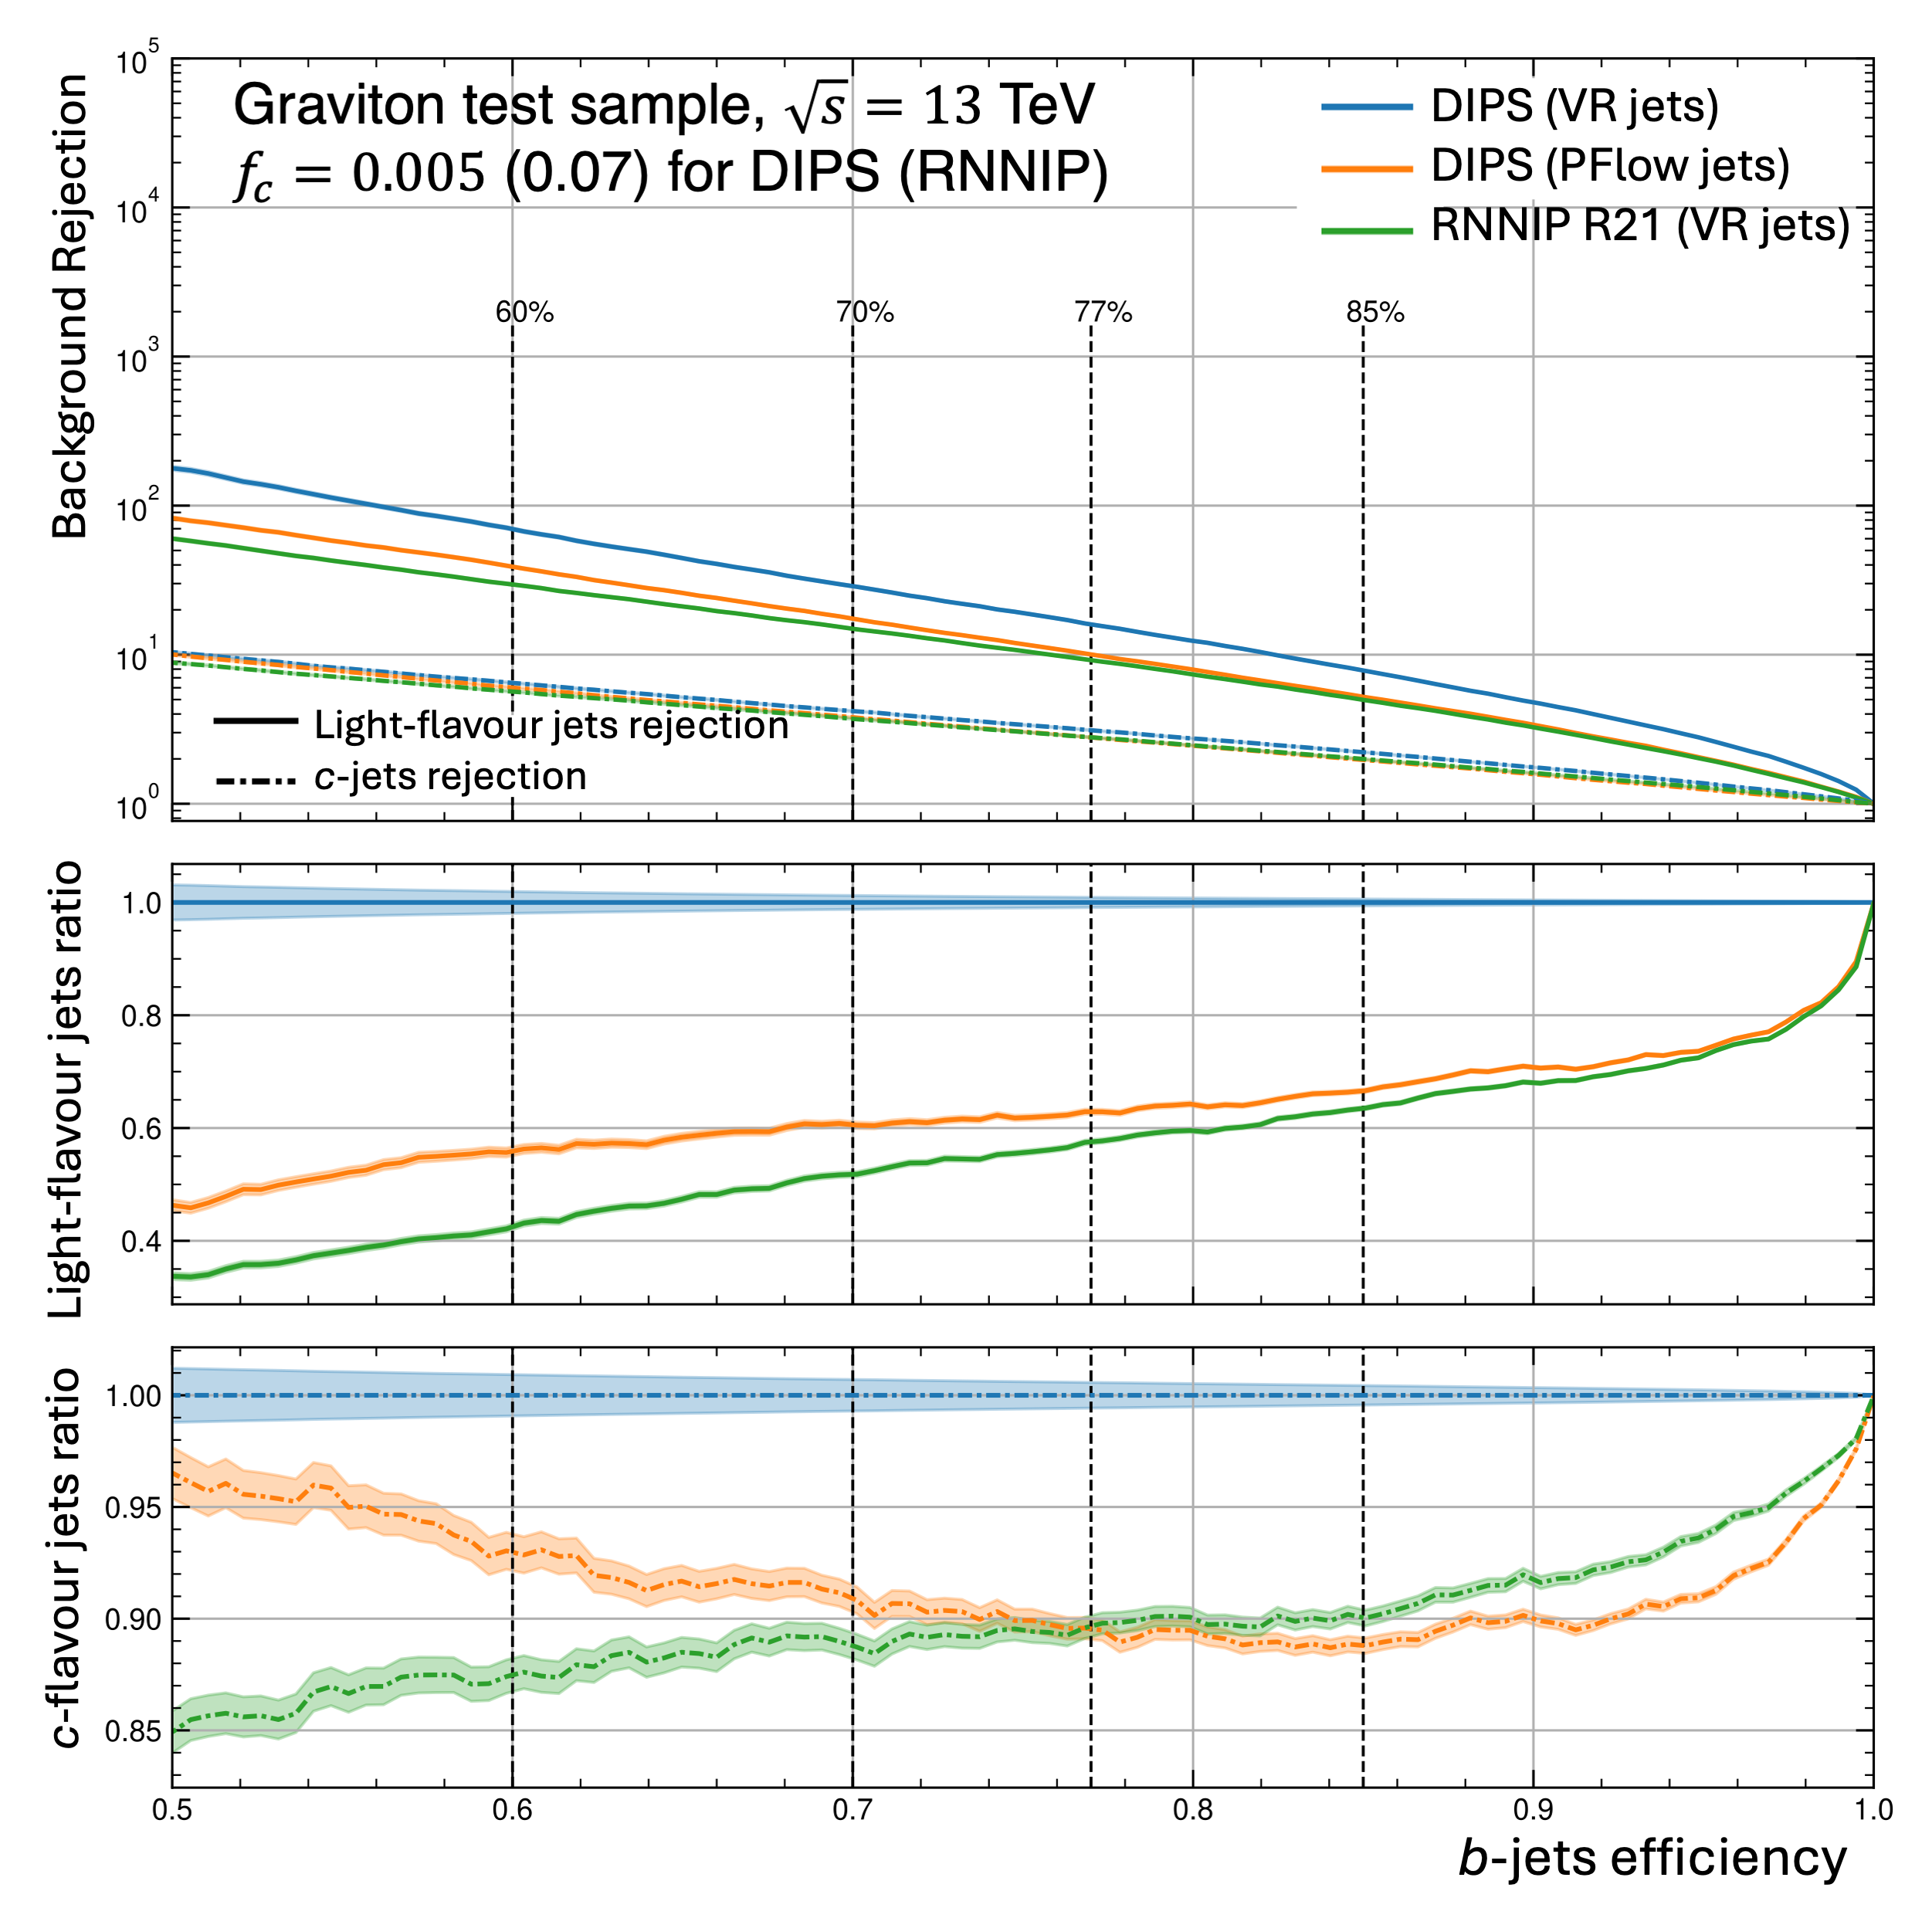
\includegraphics[scale=0.43]{Images/FTAG/VRDips/ROC/grb.png}
    \caption{Graviton test sample $b$-tagging.}
    \label{fig:dipsVRROCgr}
  \end{subfigure} \\
  \begin{subfigure}[t]{0.3\textwidth}
    \centering
    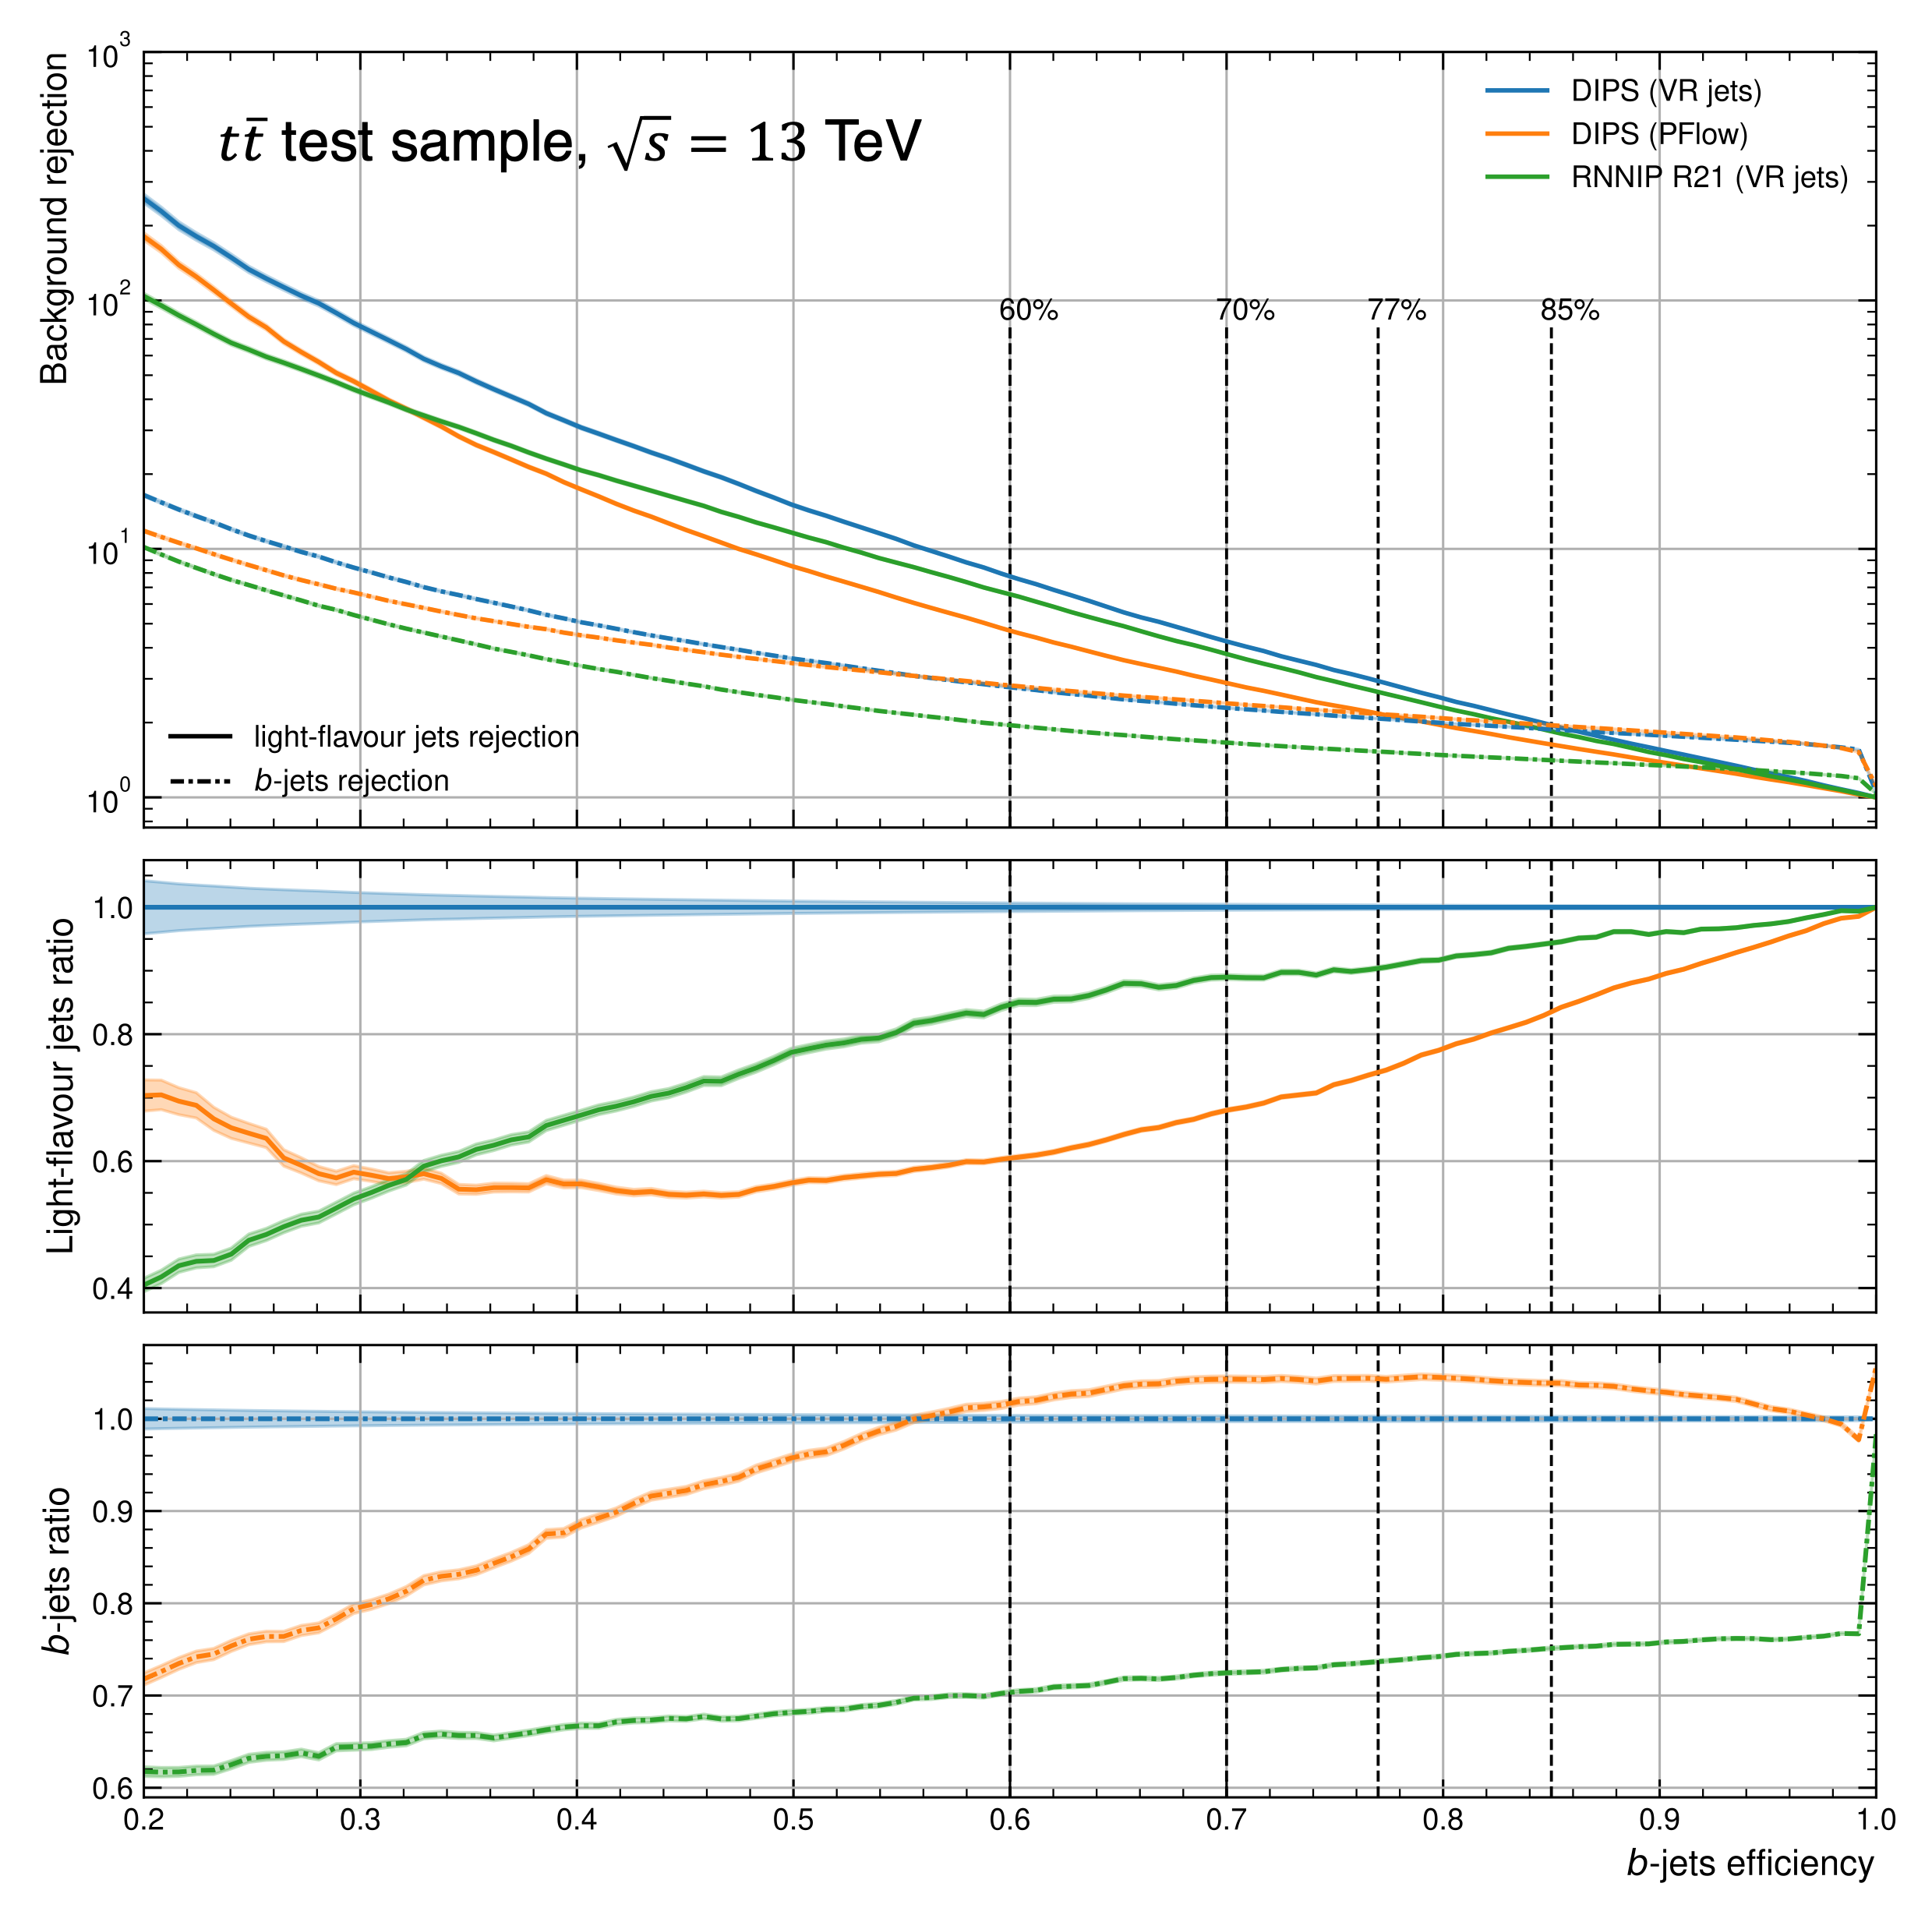
\includegraphics[scale=0.43]{Images/FTAG/VRDips/ROC/ttc.png}
    \caption{$t\bar{t}$ test sample $c$-tagging.}
    \label{fig:dipsVRROCttc}
  \end{subfigure}
  \hfill
  \begin{subfigure}[t]{0.3\textwidth}
    \centering
    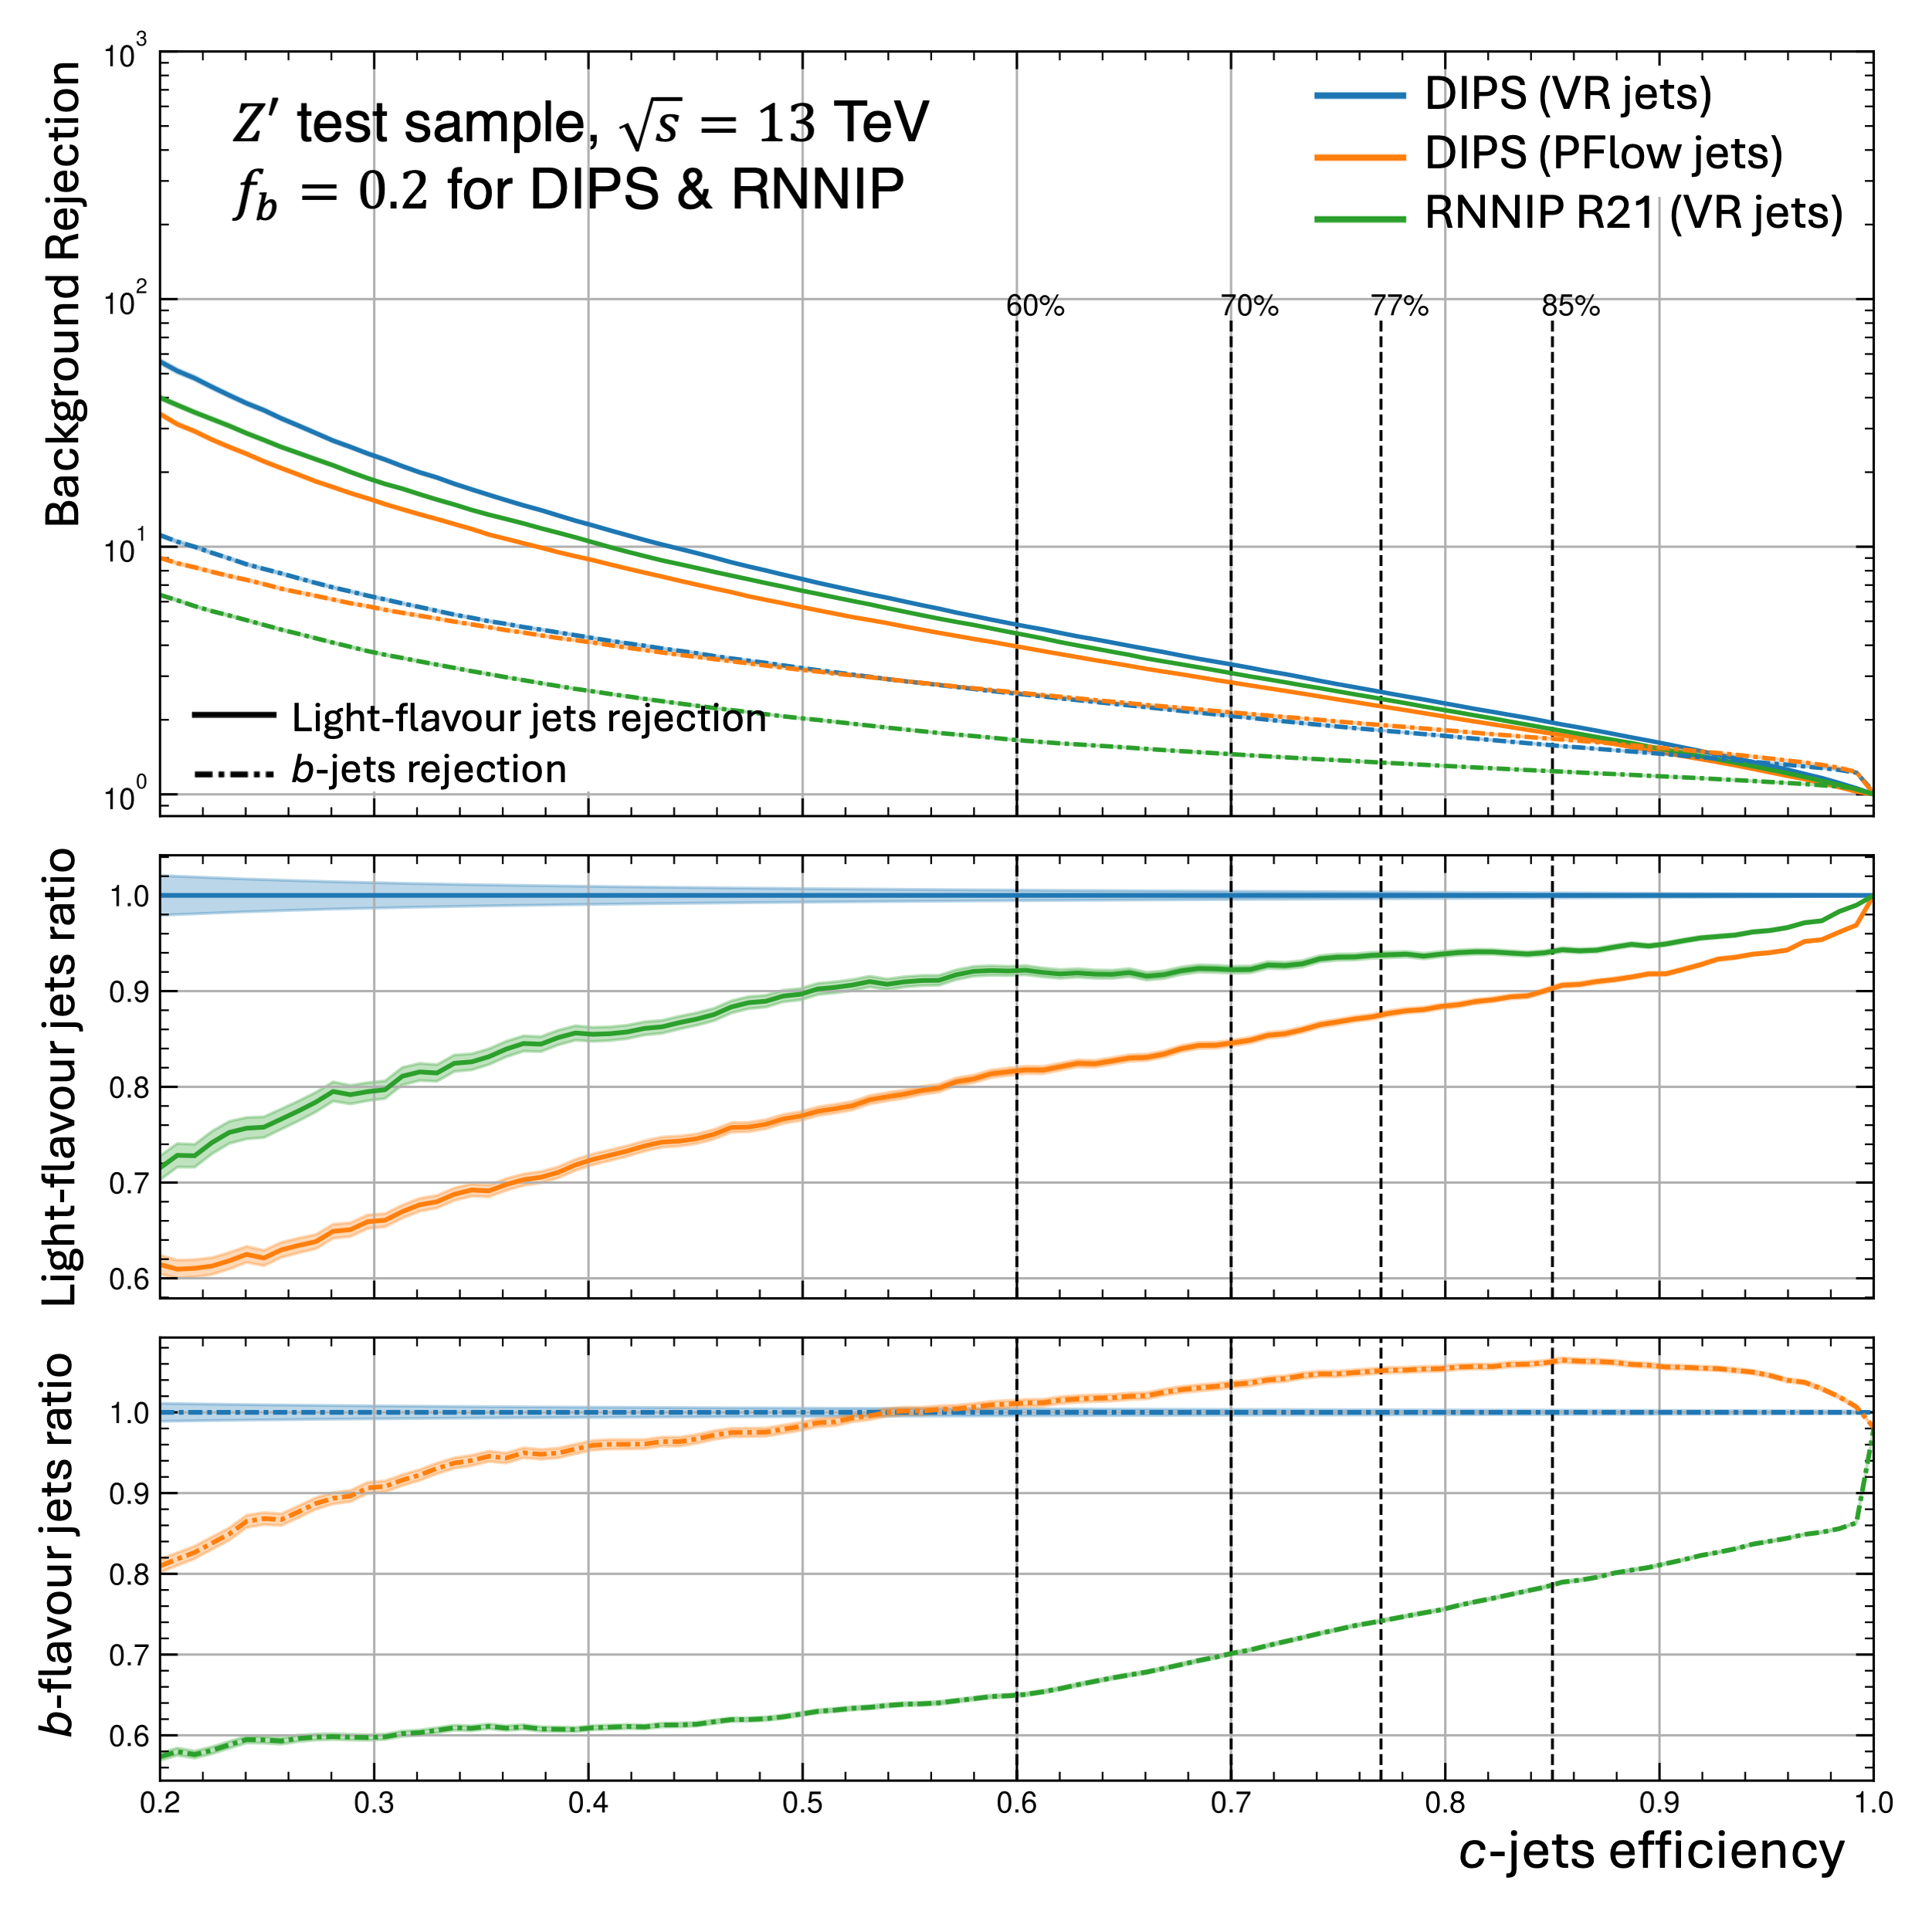
\includegraphics[scale=0.43]{Images/FTAG/VRDips/ROC/zpc.png}
    \caption{$Z'$ test sample $c$-tagging.}
    \label{fig:dipsVRROCzpc}
  \end{subfigure}
  \hfill
  \begin{subfigure}[t]{0.3\textwidth}
    \centering
    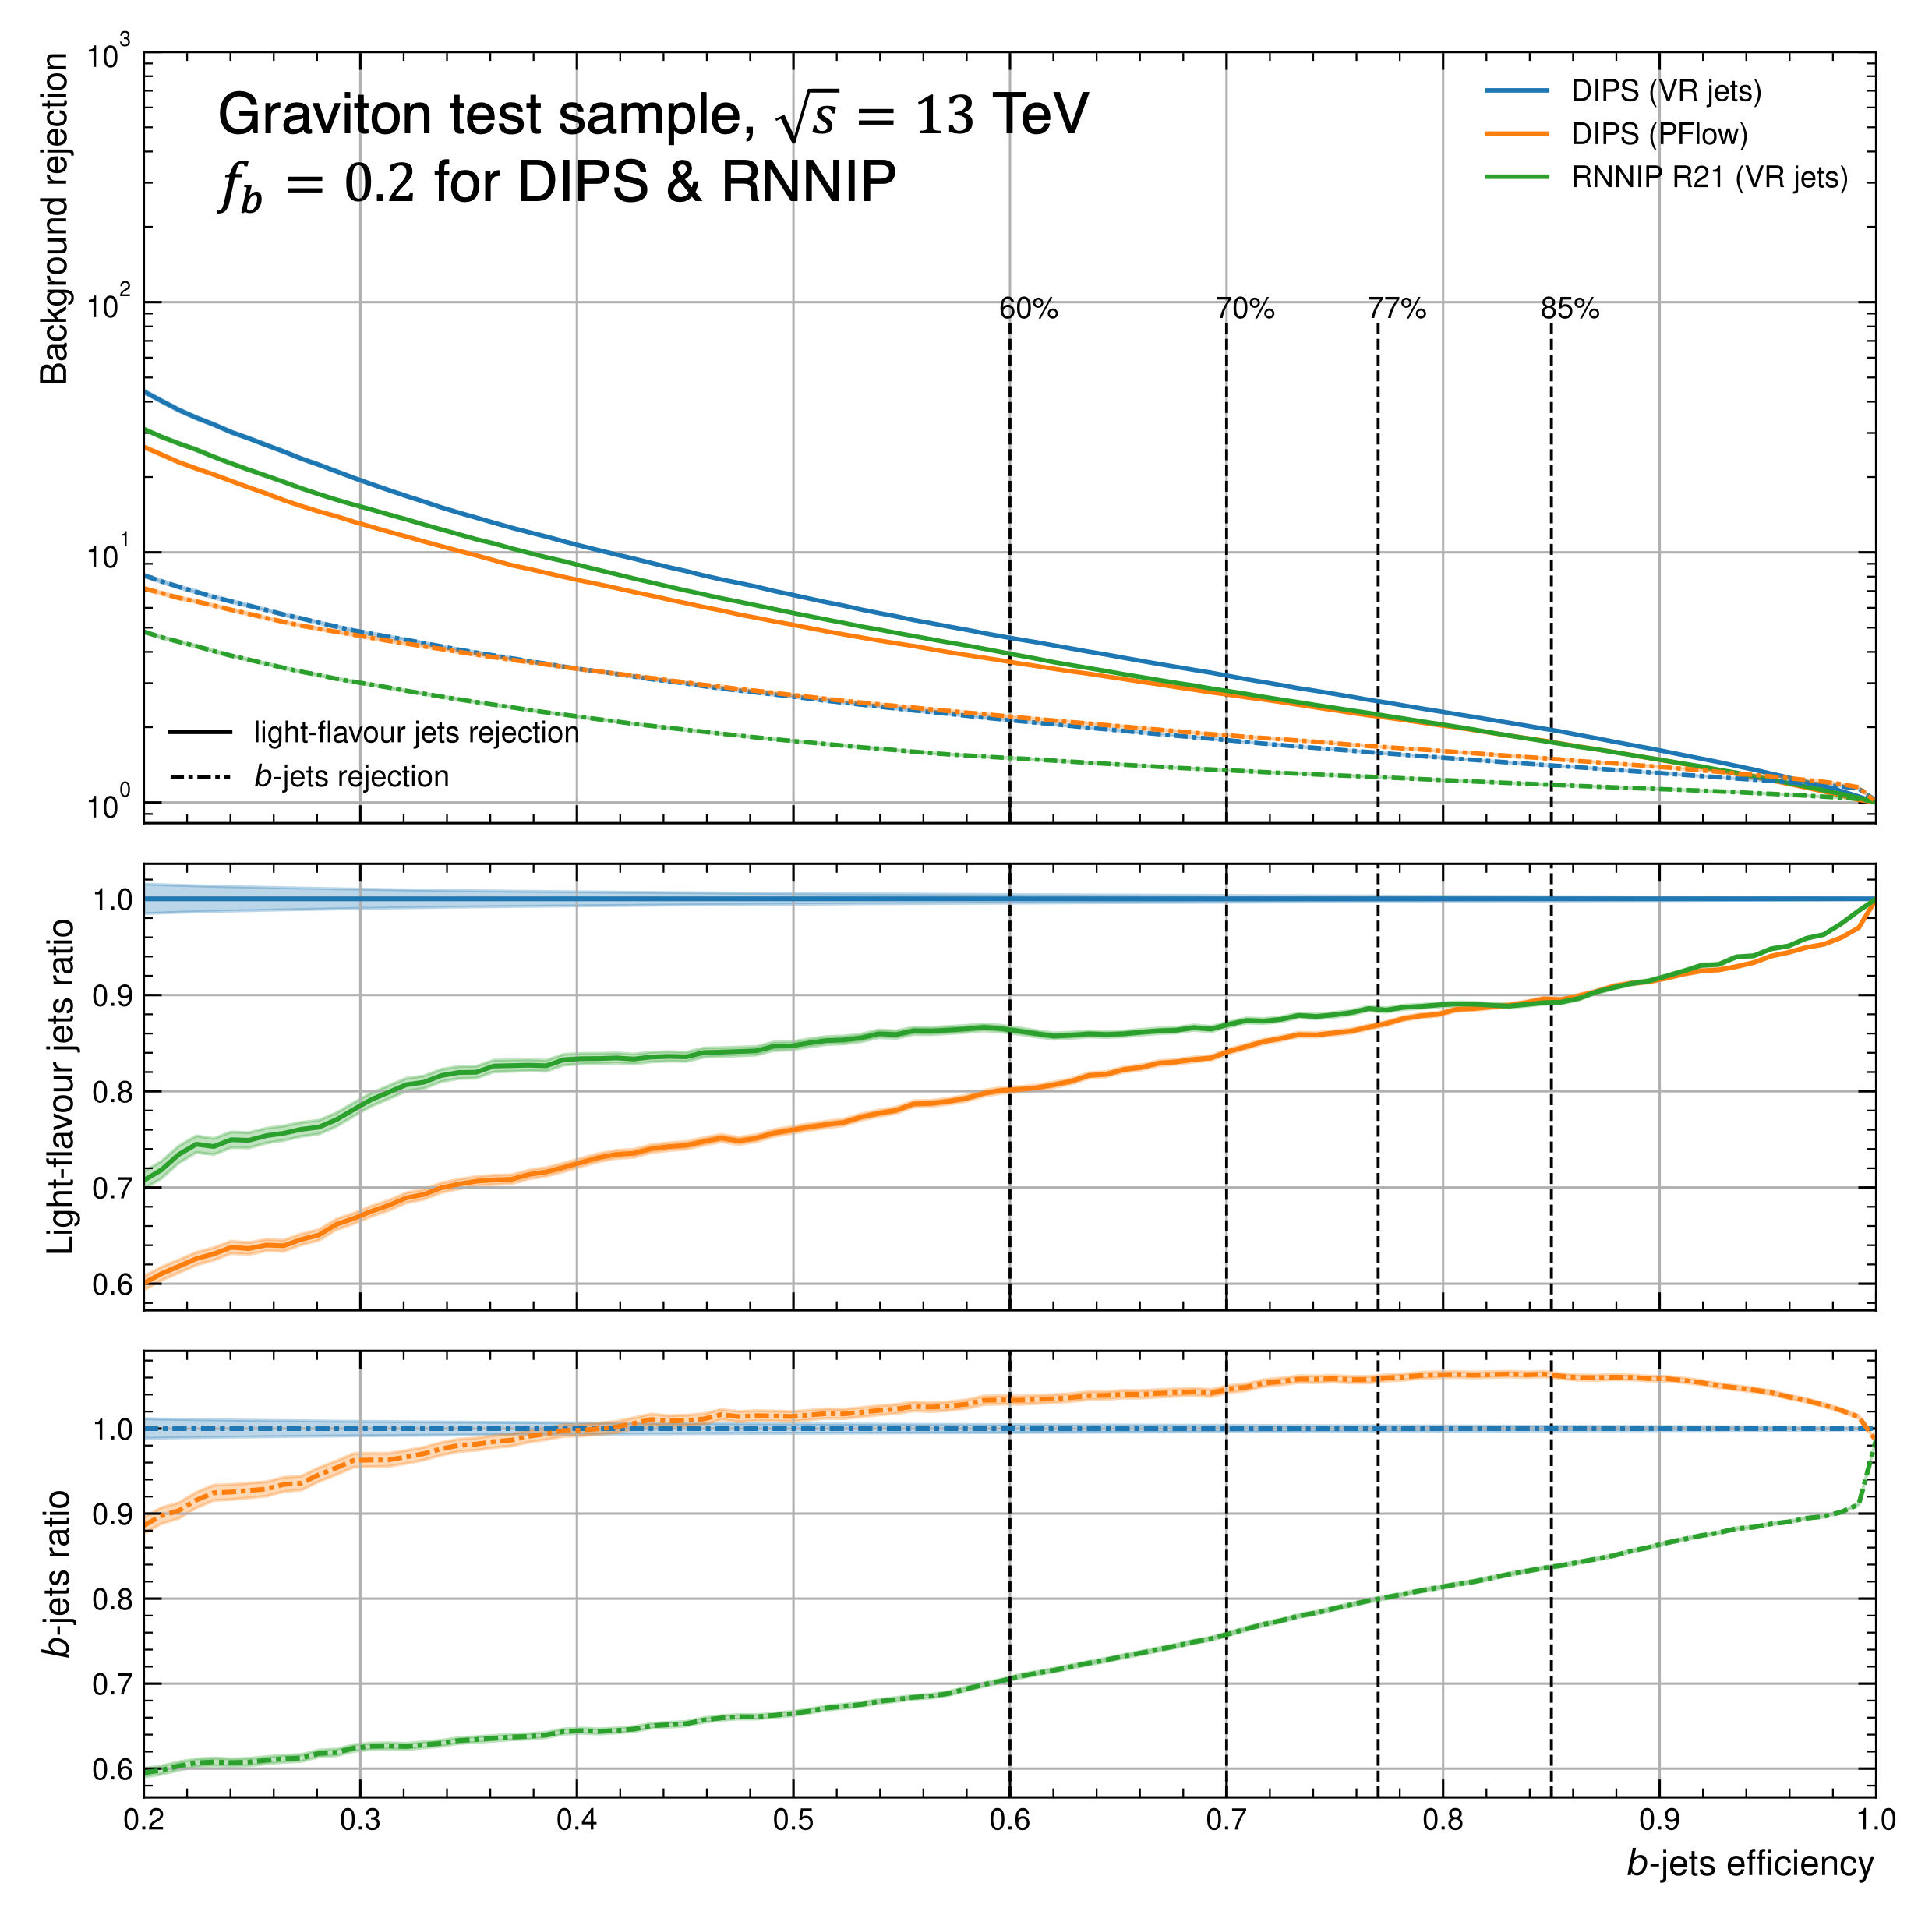
\includegraphics[scale=0.43]{Images/FTAG/VRDips/ROC/grc.png}
    \caption{Graviton test sample $c$-tagging.}
    \label{fig:dipsVRROCgrc}
  \end{subfigure}
  \caption{\gls{roc} curves for $b$-tagging (top) and $c$-tagging (bottom) on test samples of 300 k jets for $t\bar{t}$ (left), $Z'$ (centre), and the graviton process (right). Models are displayed as curves of different colours, with the \gls{vr}-jets \gls{dips} in blue, the \gls{dips} model trained on PFlow jets in orange, and \gls{rnnip} trained on \gls{vr}-jets from the previous software release R21 in green.}
  \label{fig:dipsVRROC}
\end{sidewaysfigure}

Training \gls{dips} on a dedicated set of \gls{vr}-jets clearly improves performance over relying on the PFlow-trained version, as observed by comparing the blue (\gls{vr}-trained \gls{dips}) to orange curves (PFlow-trained \gls{dips}). At a $b$-tagging efficiency of 77\%, the light-rejection is PFlow-trained \gls{dips} is indeed roughly 40\% lower. However, the $c$-rejection does not benefit as much, being either on par or even lower for the \gls{vr}-trained \gls{dips} on the $t\bar{t}$ samples. This difference in performance indicates an inappropriate choice of $f_c$ value for the $b$-tagging discriminant of the \gls{vr}-trained \gls{dips}. A so-called \textit{flavour fraction scans}, displaying the rejections at a fixed tagging efficiency for different value of the flavour fraction, can lead to a better choice for a balanced improvement in both background jet rejections. However, \gls{dips} probabilities are not meant to be used directly as discrimant but rather passed on to the high level algorithm \gls{dl1d}, hence this optimisation is reserved for the final model as presented in Chapter \ref{sec:VRdl1dTrain}. Figures \ref{fig:dipsVRROCttc} to \ref{fig:dipsVRROCgrc} lead to similar conclusions for $c$-tagging.

\subsection{Training of DL1d \& DL1r with PFlow for Run 3}
The ATLAS Collaboration continuously updates its software, updating specific methods to adopt new techniques, maintaining its many tools and adding capabilities. In preparation for the current Run 3 of the \gls{lhc} that started in 2022, ATLAS improved its reconstruction software from release 21 (R21) to release 22 (R22). As such, important elements used by flavour tagging methods have changed, requiring to retrain all taggers to ensure optimal performance under the new conditions. This work presents the first ATLAS study of the retraining of \gls{dl1r} on the new release R22 and the first training of \gls{dl1d}, including the \gls{dips} sub-tagger in the high-level flavour tagging tool. Other important novelties of this work are the possible inclusion of $\tau$-jets in the \gls{dl1} model's predictions and a new technique to efficiently process the training data into high statistics dataset using importance sampling, as mentioned in the previous section. The interest of including $\tau$ stems from their tendency to be miss-classified as $c$-jets when hadronically decaying, as both particles commonly leave three particles in the detector. The resulting taggers are observed to efficiently identify $\tau$-jets thereby providing a new way to perform $\tau$-identification and improving $c$-jet tagging. However, due to the widespread use of the \gls{ftag} algorithms and the difficulties arising in calibrating a tagger with excellent rejection against $\tau$-jets, these are not included in the default version of the tagger nor in the results shown here, but are actively under study for the new generation of tagger in the GN family. \\ % Problem: reference to tau tagging but no plots ... add them?
Two samples, the $t\bar{t}$ and $Z'$ from proton-proton collisions at $\sqrt{s} = 13$, are simulated and combined in the datasets, as described in Section \ref{ftagdatasets}. For both samples, PFlow jets are reconstructed using the anti-$k_T$ algorithm with radius $R = 0.4$. These two samples are combined into a single \textit{hybrid} sample to train the taggers, with 70\% of the total number of jets coming from $t\bar{t}$ and the remaining from the $Z'$. The $t\bar{t}$ and $Z'$ samples cover, respectively, a low- and high-$p_T$ region based on a reconstructed $b$-hadron $p_T$ separation threshold of 250 GeV for $b$-jets and a jet $p_T$ of 250 GeV for non-$b$-jets. They are re-sampled to have the same $p_T-|\eta|$ distributions, as described in the next paragraph. The relative proportion of each sample was chosen to avoid any discontinuity in the $p_T$ spectrum at their junction, as evidenced in Figure \ref{fig:distTraining}. The final evaluation of the performance of a trained tagger is performed on separated test sets of both processes and unfolded over the flavours.\\

\begin{figure}[h!]
  \center
  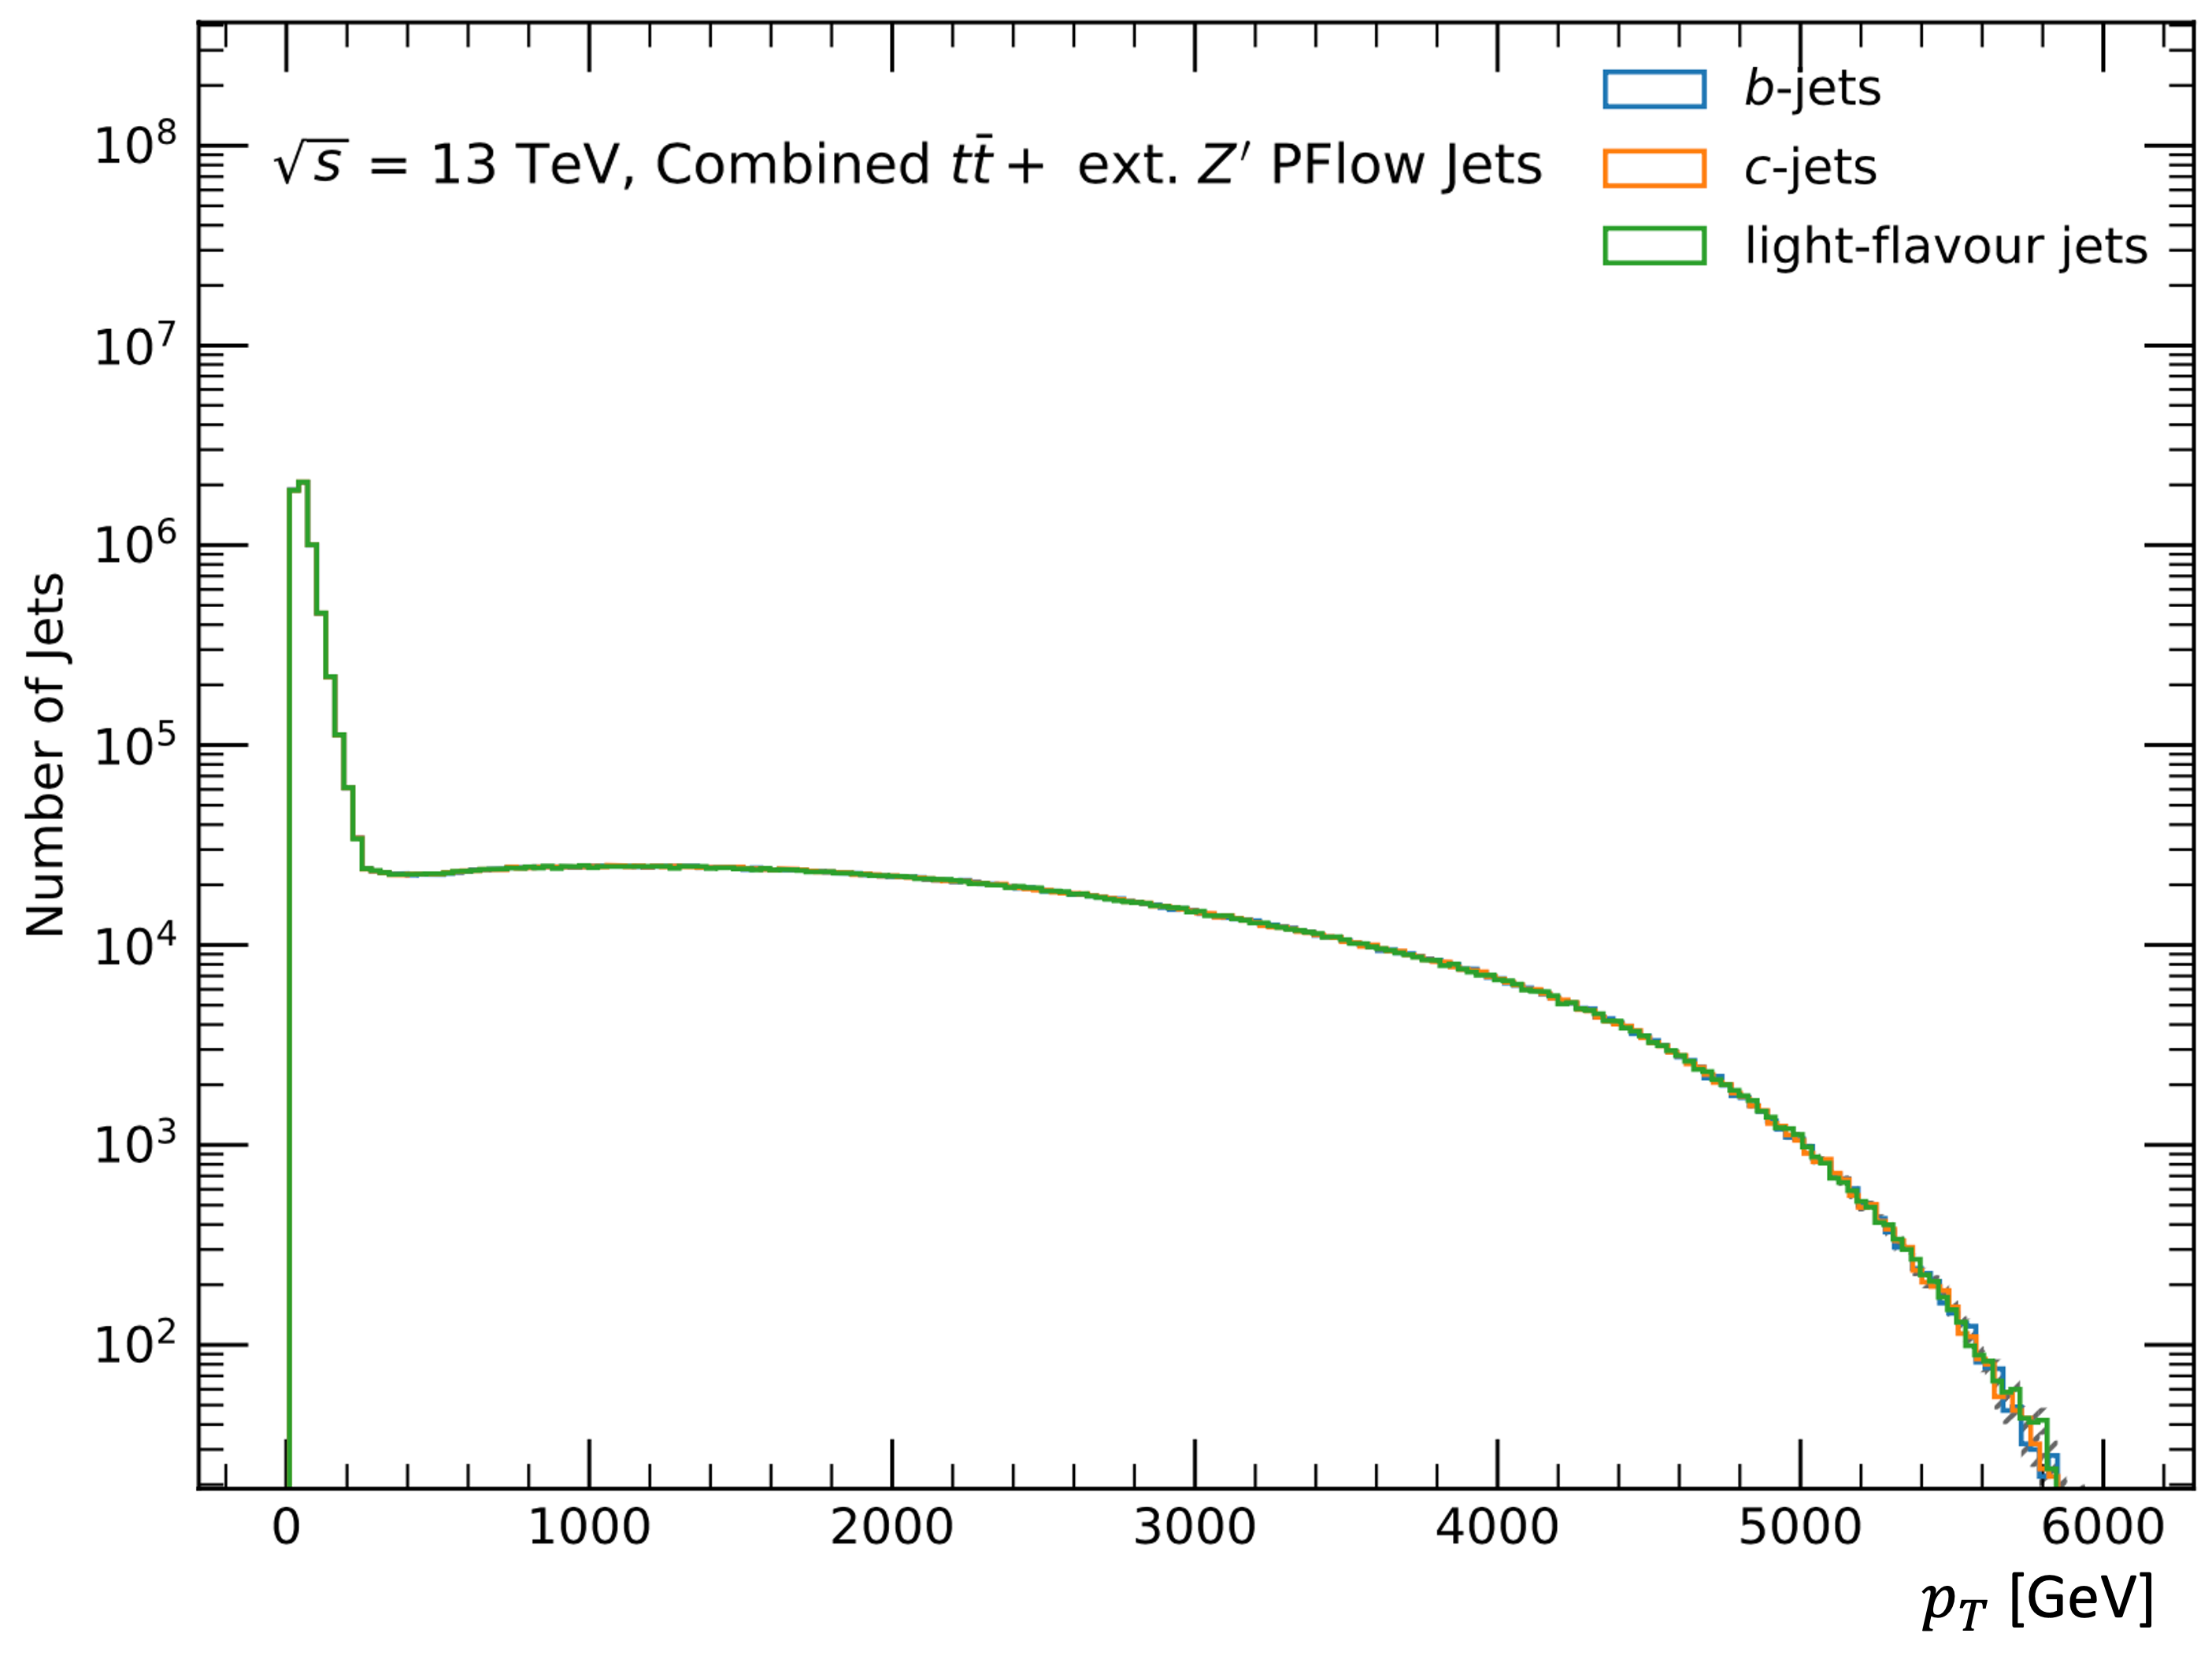
\includegraphics[width=0.48\textwidth]{Images/FTAG/DL1d/ptdist.png}
  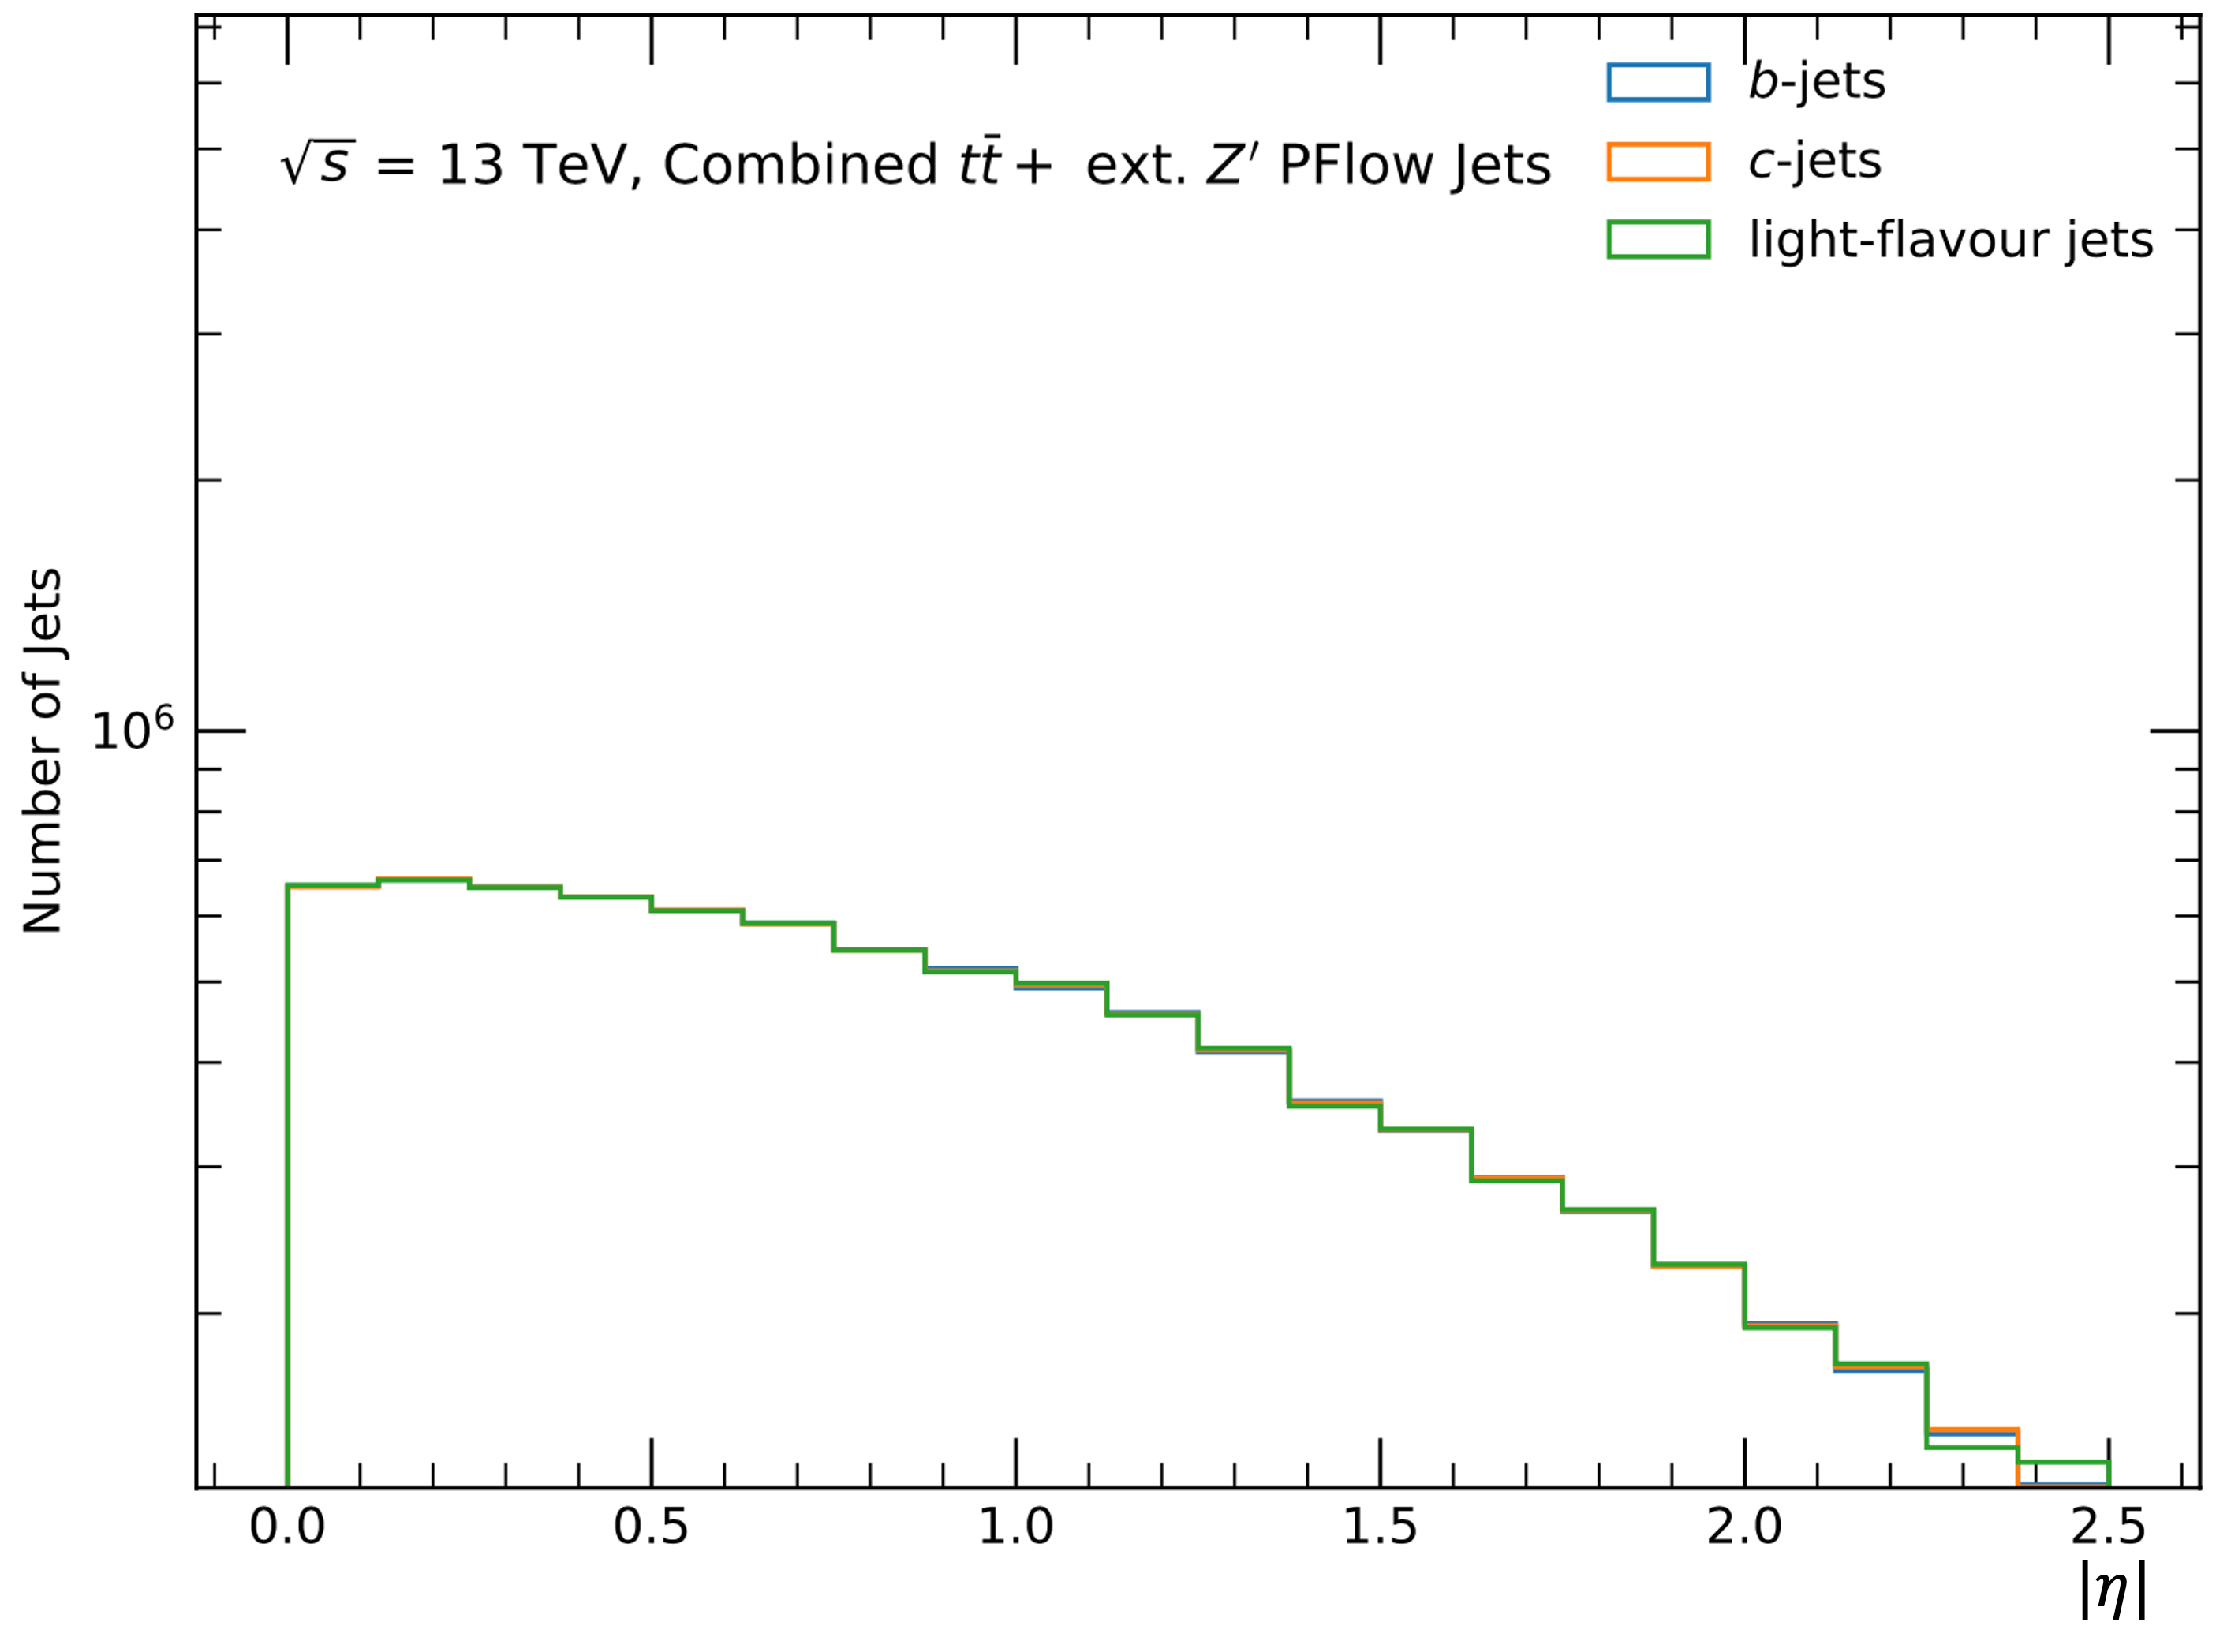
\includegraphics[width=0.48\textwidth]{Images/FTAG/DL1d/etadist.png}
  \caption{The $p_T$ (left - in MeV) and $|\eta|$ distributions of the resampled $b$-, $c$-, and light-jets in, respectively, blue, orange, and green. The three ses are resampled to have the same $p_T-|\eta|$ 2D distributions. The flat $p_T$ spectrum extending up to several TeV is due to the exotic $Z'$ process generated with varying mass, starting at 150 GeV. The large peak at lower $p_T$ is the $t\bar{t}$-process. These sets have 8.3 million jets per flavour.} 
  \label{fig:distTraining}
\end{figure}

ATLAS flavour tagging tools are widely used across the Collaboration. It is therefore essential for the taggers not to learn specific features of the processes simulated but to focus on the inherent differences between the studied flavours in order to generalise to other processes. An effective way to limit the importance of the simulated processes is to downsample the hybrid sample in [$p_T - \eta$] bins to have the same number of $b$-, $c$-, and light-jets in each 2D bin. This removes the distinction of kinematic phase space between each flavour due to the process specific physics. To avoid biasing the output of the tagger towards the most likely flavours in the process, each jet-flavour is also required to be equally likely in the training set, a requirement satisfied by having the same yield of $b$-, $c$-, and light-jets. Applying this technique, the total statistics available for the R22 training is of $25 \times 10^{6}$ jets per flavour for training. The $t\bar{t}$ and $Z'$ samples for validation and testing are each made of 1 million jets and are not downsampled to have the same [$p_T - \eta$] distribution nor the same yield of different flavours: they represent a realistic distribution of the underlying processes. The main limitator when downsampling are $c$-jets, as all $c$-jets from the $t\bar{t}$ process are selected which limits the amount of $b$- and light-jet that can be taken. This process is extremely wasteful, using only 17\% (11\%) of all available $b$-jets (light-jets) in the $t\bar{t}$ sample.\\

Training is done with the \uppercase{Umami} framework \cite{UmamiCite} based on TensorFlow \cite{tensorflow2015-whitepaper} for 300 epochs with a variable learning rate schedule and the default network structure adopted in the previously released \gls{dl1r} (R21): 8 fully connected \gls{nn} of smoothly-decreasing sizes in [256, 128, 60, 48, 36, 24, 12, 6] with \gls{relu} activation leading to a final softmax layer producing the predicted probabilities for each flavour. While the \gls{dips} probabilities used as inputs to \gls{dl1d} come from a model trained on the new release, the \gls{rnnip} probabilities are still from a model trained on the previous one (R21) \cite{ATL-PHYS-PUB-2017-003, ATL-PHYS-PUB-2020-014}. Indeed, due to its significantly lower performance, \gls{rnnip} is no longer supported in the new release and is included for sake of comparability to the previous techniques. The models at an epoch offering the best combined results in terms of $b$-tagging efficiency and rejection from $b$-jets on the validation set are selected for further analysis. Importantly, every training converged to a fixed set of performance values, with no overtraining occurring.\\

Several modifications to the model architecture, list of input variables, and preprocessing and training procedures have been explored, with no significant gain observed:
\begin{itemize}
\item The preprocessing steps were revised to reduce the size of the evaluation sets for the benefit of the training one. A dual approach, downsampling light-jets and upsampling $c$-jets to the $b$-jets [$p_T - \eta$], has also been implemented. As previously described, this approach uses importance sampling with replacement to obtain the same fraction of the different flavours and the same $p_T$ and $|\eta|$ distribution. While the performance of the majority classes was observed to improve, the efficiency at tagging the upsampled minority class ($c$-jets) was slightly lower. This trade-off can be compensated by modifying the flavour fractions and thus does not result in any significant performance changed. This is likely due to the model saturating its performance given the large dataset already available. Other models, such as those from the GN family that have more parameters, have however been observed to make gains from the importance sampling approach.
\item Several modifications to the list of input features have been attempted, with no clear advantage uncovered. Adding pile-up information (the actual number of interactions per crossing and the number of primary vertices were tested) was not observed to have an impact on the tagging efficiency. Adding other variables from \gls{sv1} or JetFitter was also not observed to improve performance. However, a positive observation is that the IP2D and IP3D taggers can both be safely removed without changes to the performance, as the information they add is in all likelihood now covered by the \gls{dips} sub-tagger, thereby reducing the list of sub-taggers to maintain and simplifying the architecture.
\item The structure of the network and its training procedure, leveraging transfer learning. Using samples produced with an older release of the ATLAS software (R21) to pre-train the model was not observed to deliver a boost in performance when later training on the new release (R22). Changing the size of the network and the batch size was also not observed to have a positive effect.
\end{itemize}

The conclusion driven by the lack of improvements from these three attempts is that models built on this simple \gls{dnn} structure with large dataset are already likely saturating their performance from the set of inputs. The performance of the retrained \gls{dl1r} tagger on the new release was found to be in good agreement with the at-the-time released \gls{dl1r}, despite using the same training of \gls{rnnip} on the previous release. In order to establish a meaningful benchmark for the newly trained taggers, the performance of the then released \gls{dl1r} tagger, trained and evaluated on an analogous set of samples from the previous release (R21), is included in the following results as benchmark under the label \textit{Recom. \gls{dl1r}}. A first look at the new family of taggers is also advertised by plotting the performance of a pre-release \gls{gn1} tagger, although this is discussed in further details in the next Chapter \ref{chap:GN}. \\

Figure \ref{fig:DL1dtt} presents the \gls{roc} curves on the $t\bar{t}$ (left) and $Z'$ (right) samples for $b$-tagging. These \gls{roc} plots show, on the $x$-axis, the $b$-tagging efficiency ($\epsilon^b_b$) versus, on the $y$-axis, the rejection $\mathcal{R}^b_Y$ for $Y \in$ [$c$, light]. The two bottom sub-plots present the ratio of the c-jet rejection and light-jet rejection curves to the blue ones. This blue curve is the recommended \gls{dl1r} performance and serves as the baseline of the comparison, while the new tagger \gls{dl1d} is plotted in orange. Figure \ref{fig:DL1dz} shows the same plots for $c$-tagging, with respect to $b$- and light-jet rejections. The important observation is the clear gain obtained when replacing \gls{rnnip} with \gls{dips}. Both the $b$- and $c$-tagging performance of \gls{dl1d} clearly dominate the \gls{dl1r} versions, with a significant improvement in background flavour rejection for all tagging efficiency considered, as summarised in Table \ref{tab:max-perf}. The largest improvement in performance is obtained for $b$-tagging on the $t\bar{t}$ process, corresponding to a lower jet momentum. This latter points to a dynamical behaviour of the \gls{dips} subtagger that can be traced back to the looser jet selection. Higher momentum jets are more likely to have a larger set of tracks and these tracks tend to be closer to each other due to relativistic boosting. The looser selection forces the \gls{dips} model enduce to sift through a larger set of noisy tracks which brings lower performance at higher momentum, while a gain is obtained at lower momentum from the nicer geometrical separation and smaller initial set.  \\

The light-rejection from $b$-jets \gls{roc} curve in Figure \ref{fig:DL1dtt} traces an elbow at high $b$-jet efficiencies. This effect is also present in the $b$-rejection from $c$-tagging, Figure \ref{fig:DL1dz}. Both correspond to a set of, respectively, light-jets and $b$-jets that do not overlap with the $b$-jets $b$-tagging and $c$-jets $c$-tagging discriminants distributions, as shown in Figures \ref{fig:scoreDL1dtt} and \ref{fig:scoreDL1dz}. These ``background`` jets are easily removed from the core set of ``signal'' jets due to inherent differences between the flavours and the discrete nature of some sub-taggers used. \\

The background rejections of the various taggers for $b$-tagging ($c$-tagging) as a function of the jet transverse momentum $p_T$ at an inclusive $b$-efficiency of 70\% ($c$-efficiency of 30\%) per region displayed are shown in Figure \ref{fig:ptDL1dtt} (Figure \ref{fig:ptDL1dz}). Throughout the $p_T$ range considered, \gls{dl1d} outperforms the \gls{dl1r} tagger. The low $p_T$ $b$-rejection from $c$-jets is noticeably better for the newly trained tagger compared to \gls{dl1r}. The discontinuity of the rejections between the two processes arises from the inclusive $b$-tagging efficiency being computed inclusively per-region and not exclusively for the whole range. 

%
\begin{center}
\begin{figure}[h!]
\centerline{
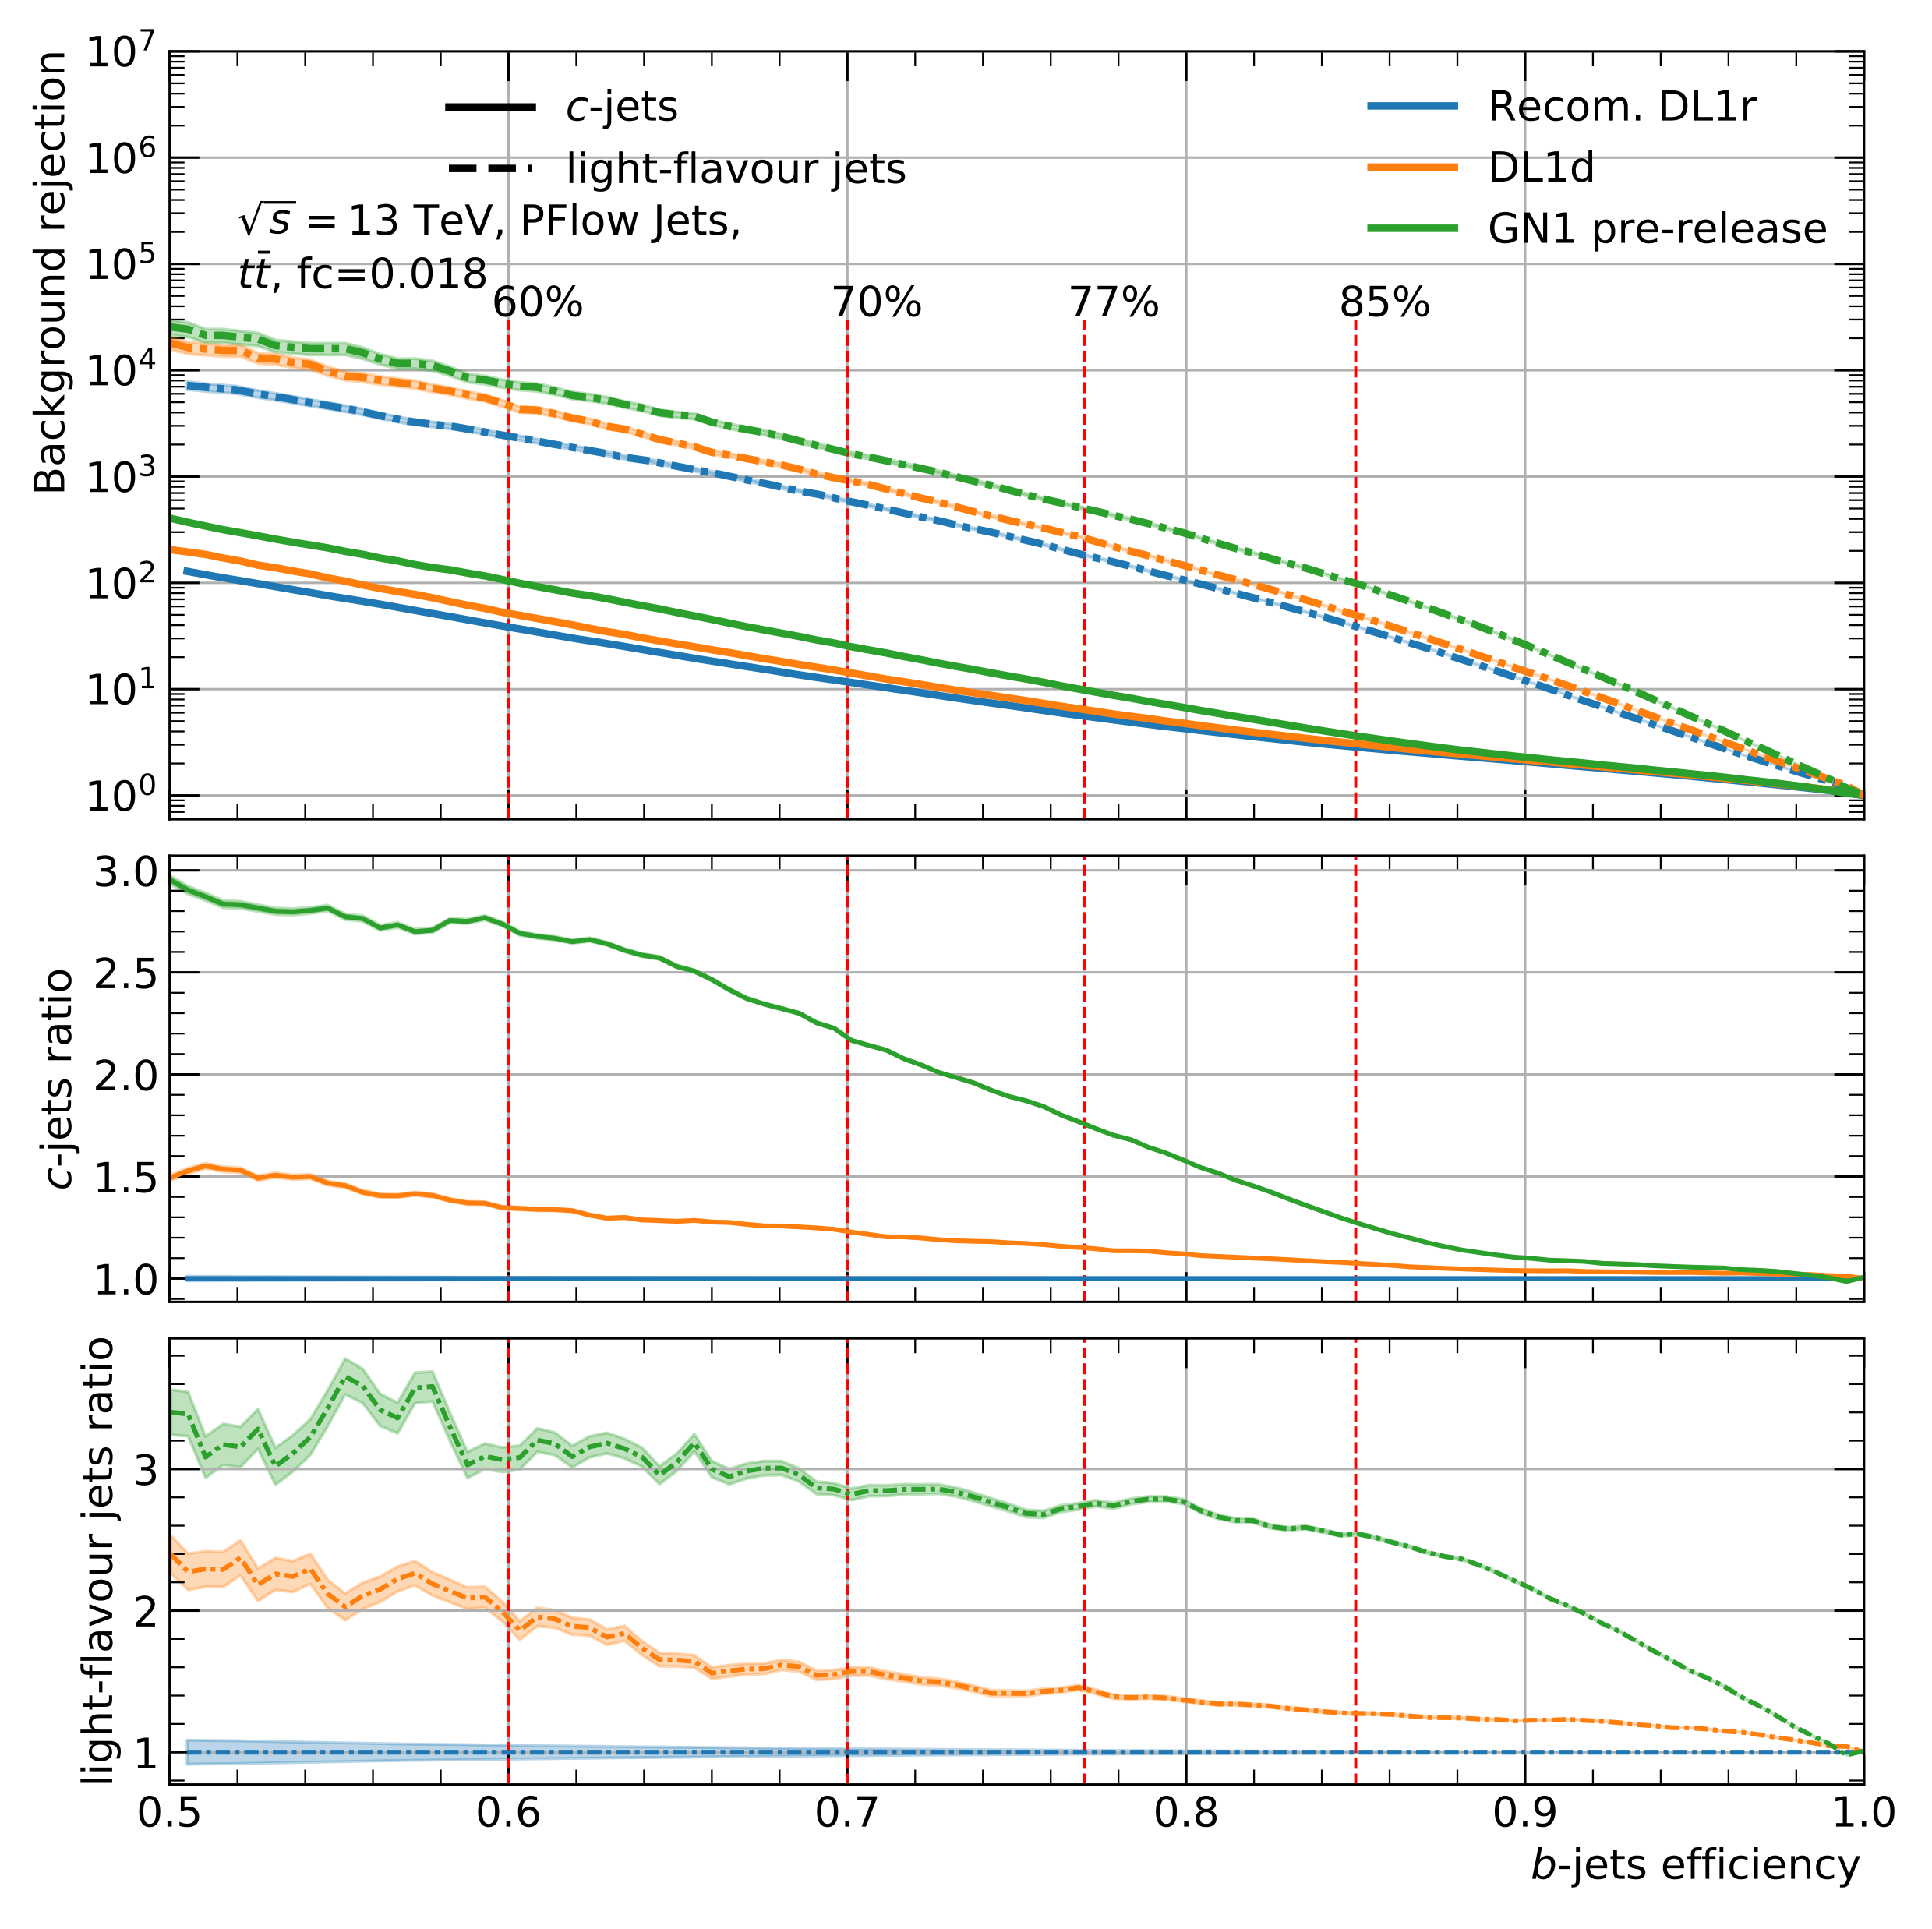
\includegraphics[scale=0.45]{Images/FTAG/DL1d/ROC/ttb.png}
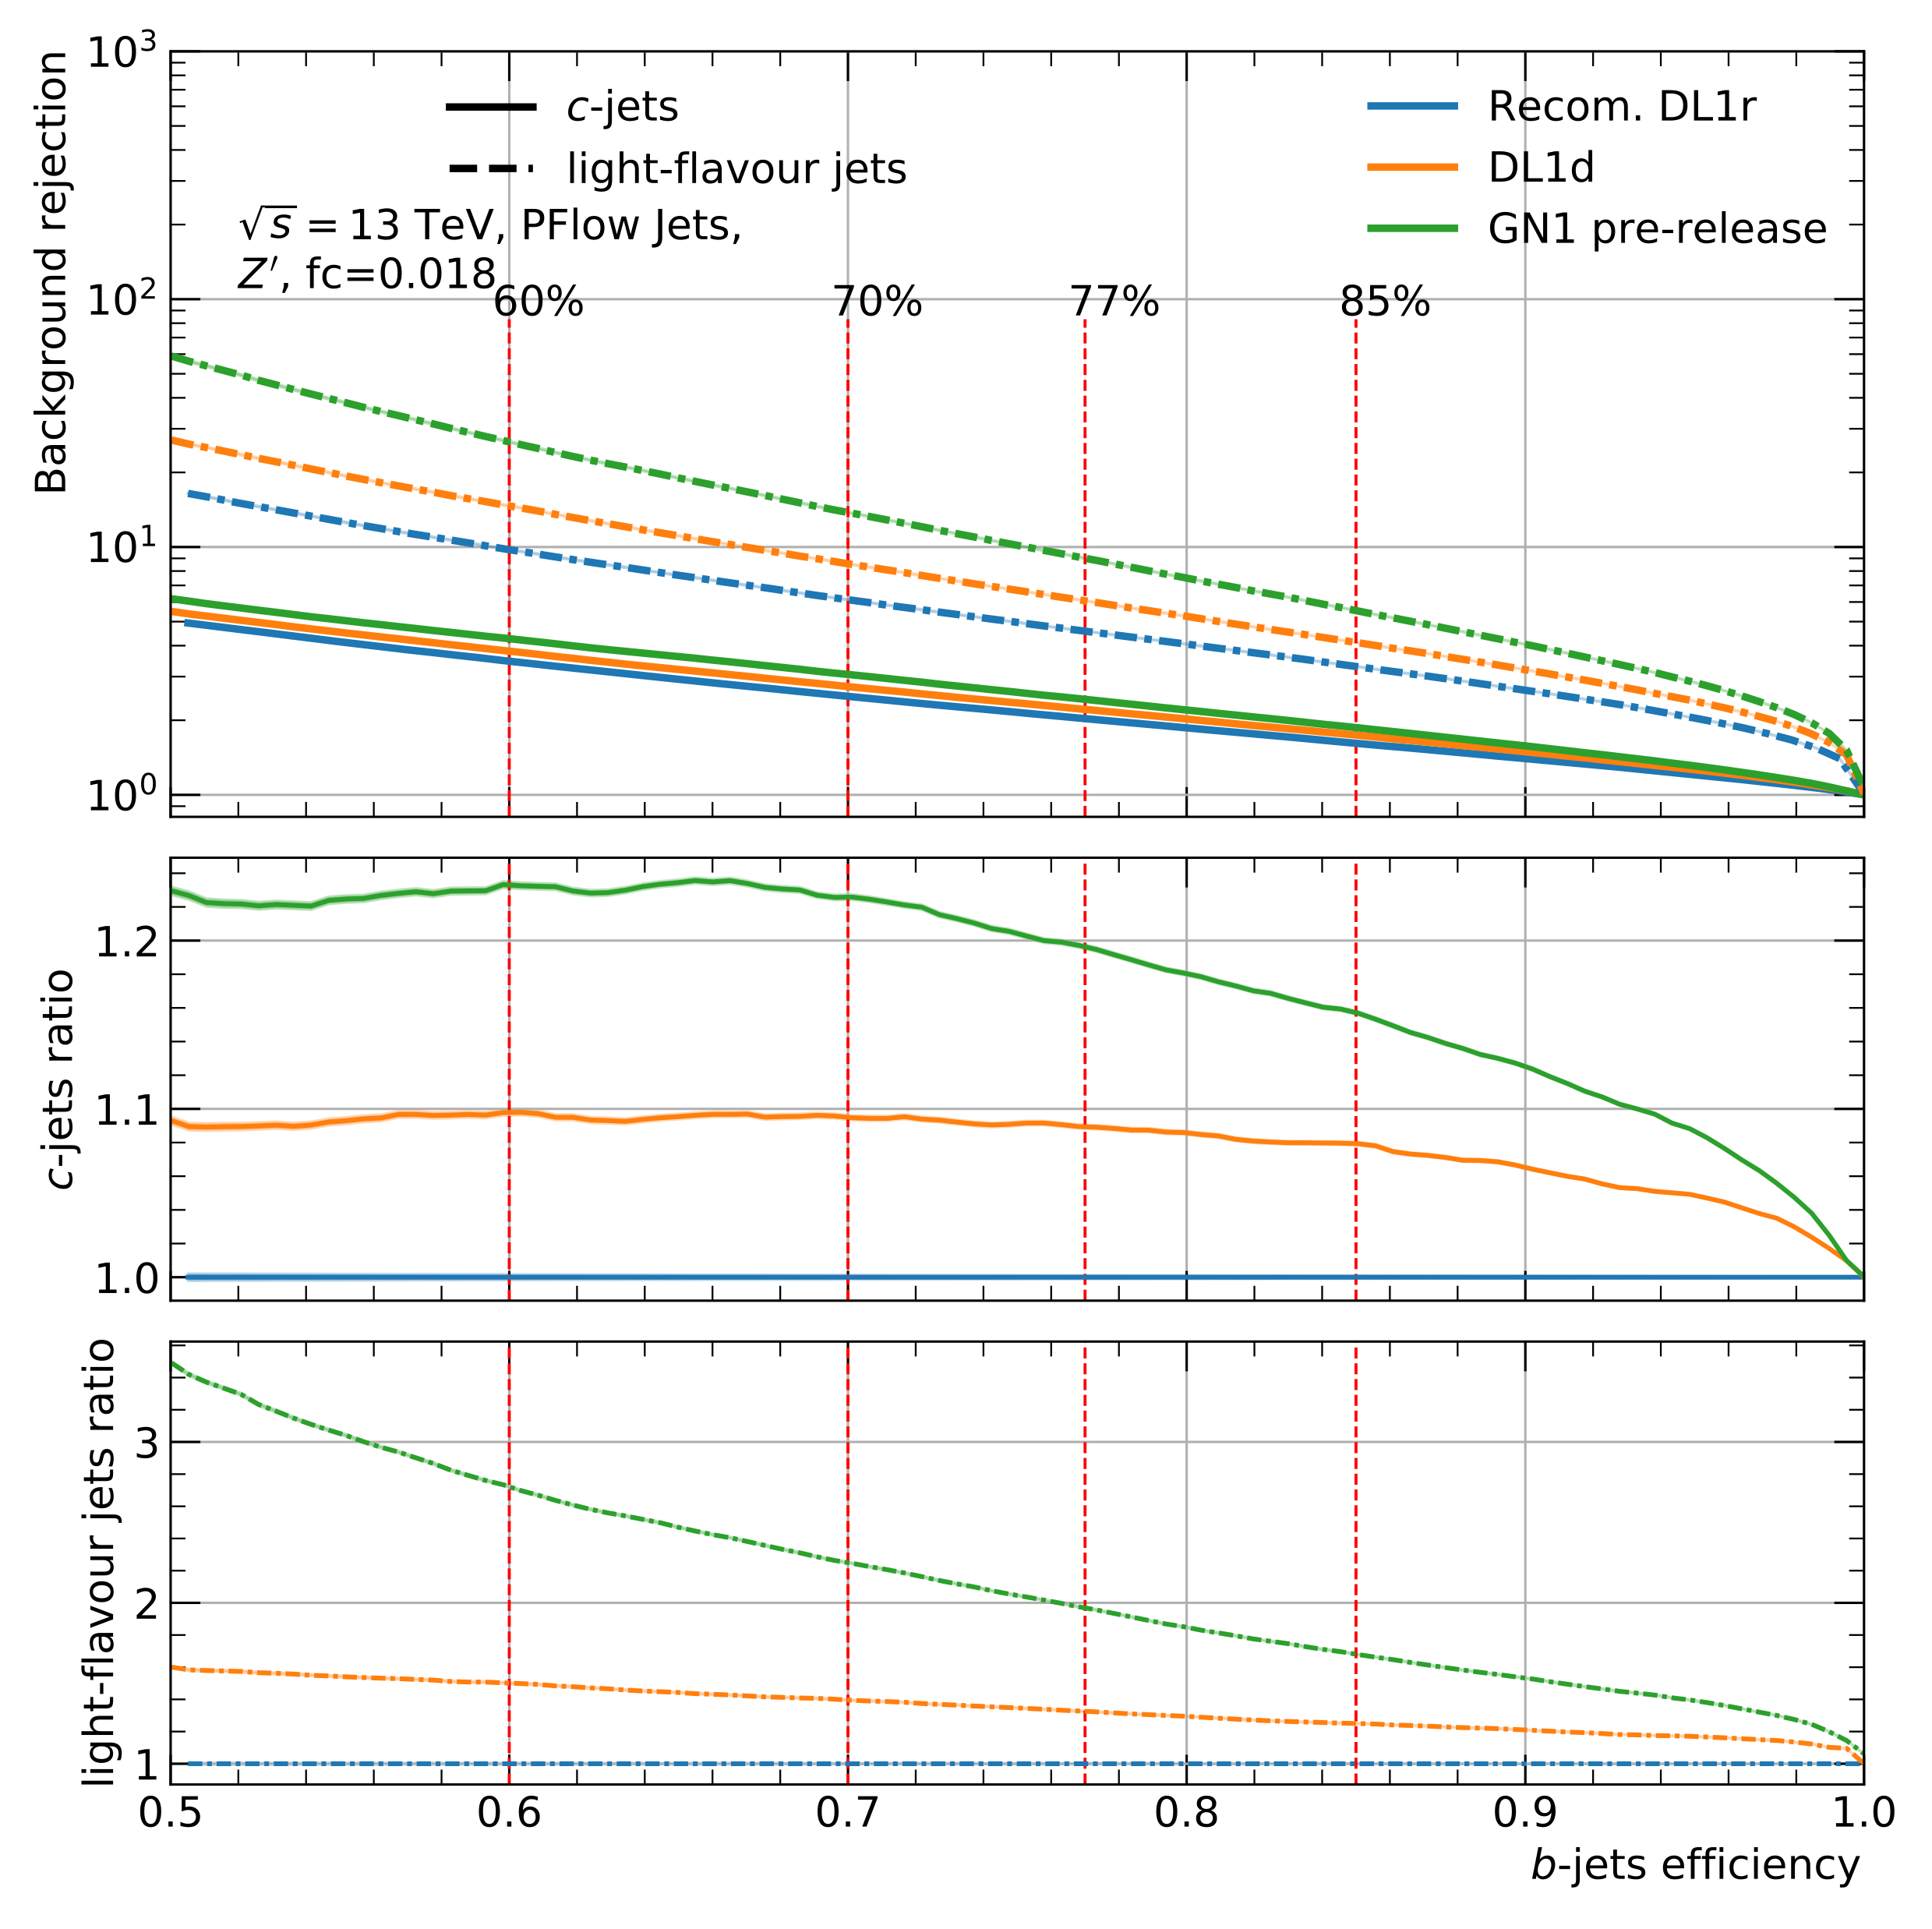
\includegraphics[scale=0.45]{Images/FTAG/DL1d/ROC/zpb.png}
}
\caption{Performance for $b$-tagging with a flavour fraction of $f^b_c = 0.018$. Left: $t\bar{t}$; right: $Z'$. Top: \gls{roc} curves; centre: ratio of $c$-jets rejection from $b$-jets relative to the R22-retrained \gls{dl1r}; bottom: same ratio for light-jets rejection. List of taggers: {\color{blue} recommended \gls{dl1r} from the previous release}; {\color{orange} \gls{dl1d} trained on the new release}; {\color{greenforest} \gls{gn1} test-model trained on the new release}.}
\label{fig:DL1dtt}
\bigskip
\centerline{
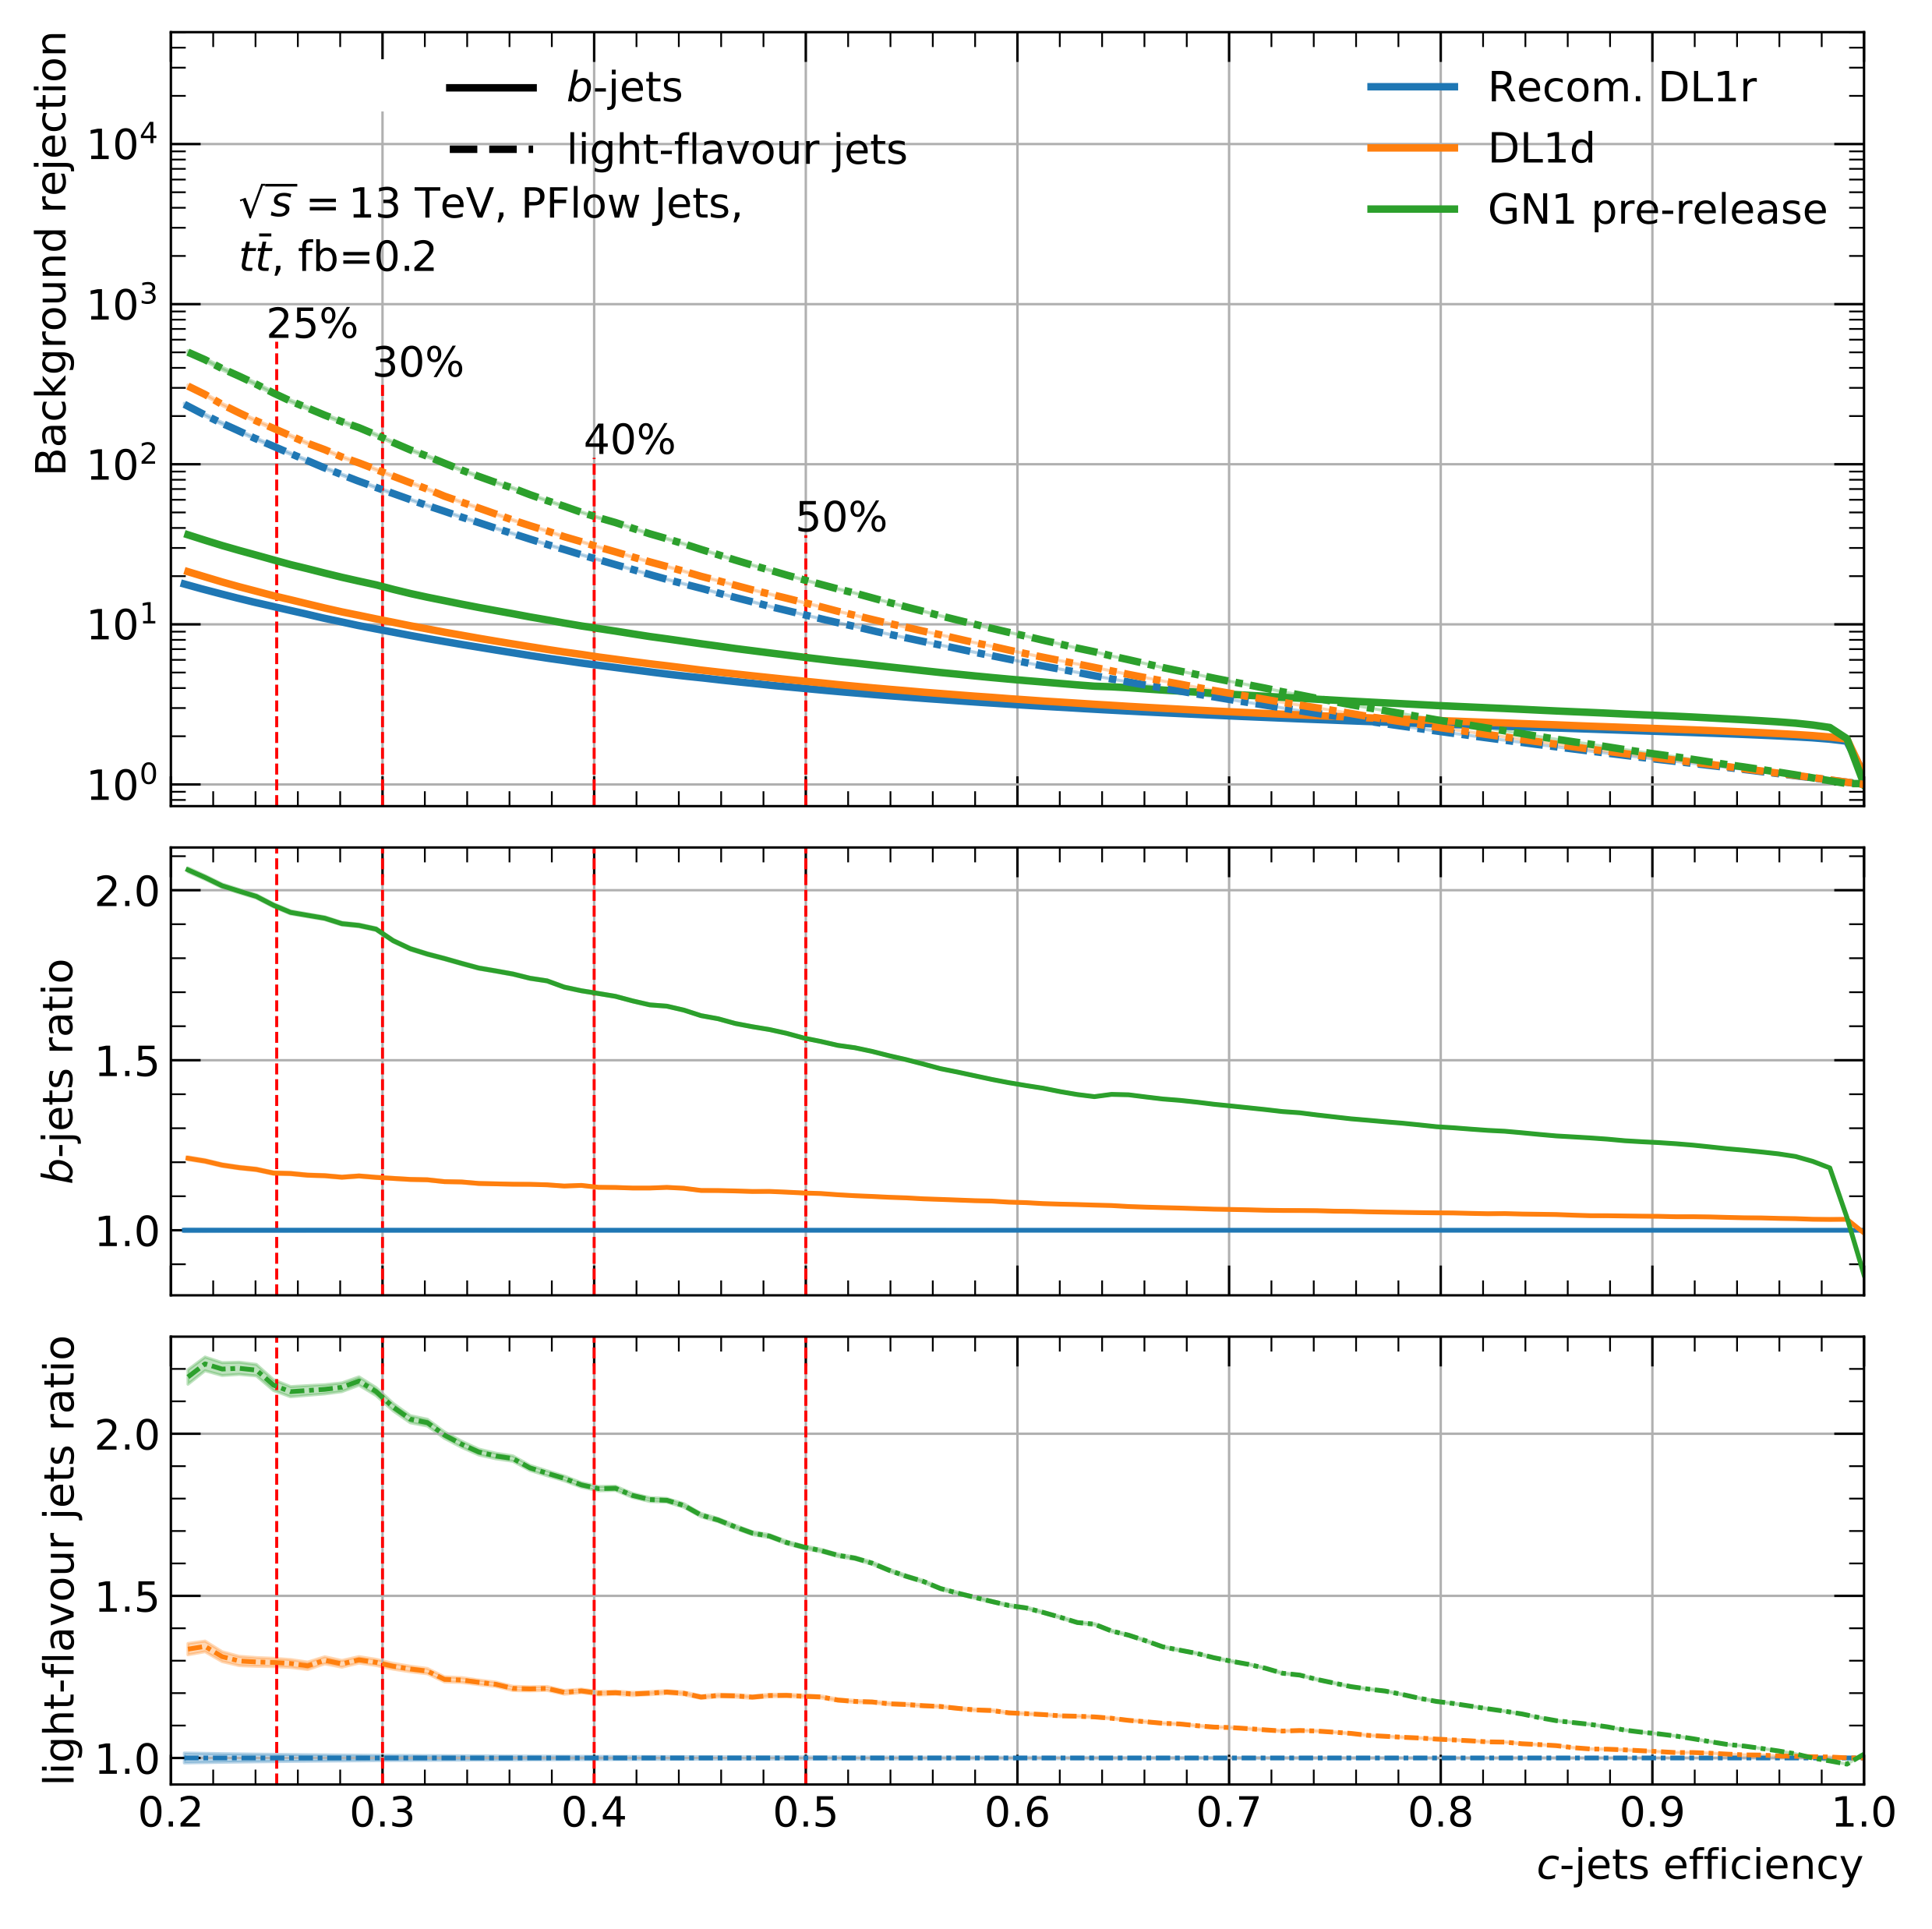
\includegraphics[scale=0.45]{Images/FTAG/DL1d/ROC/ttc.png}
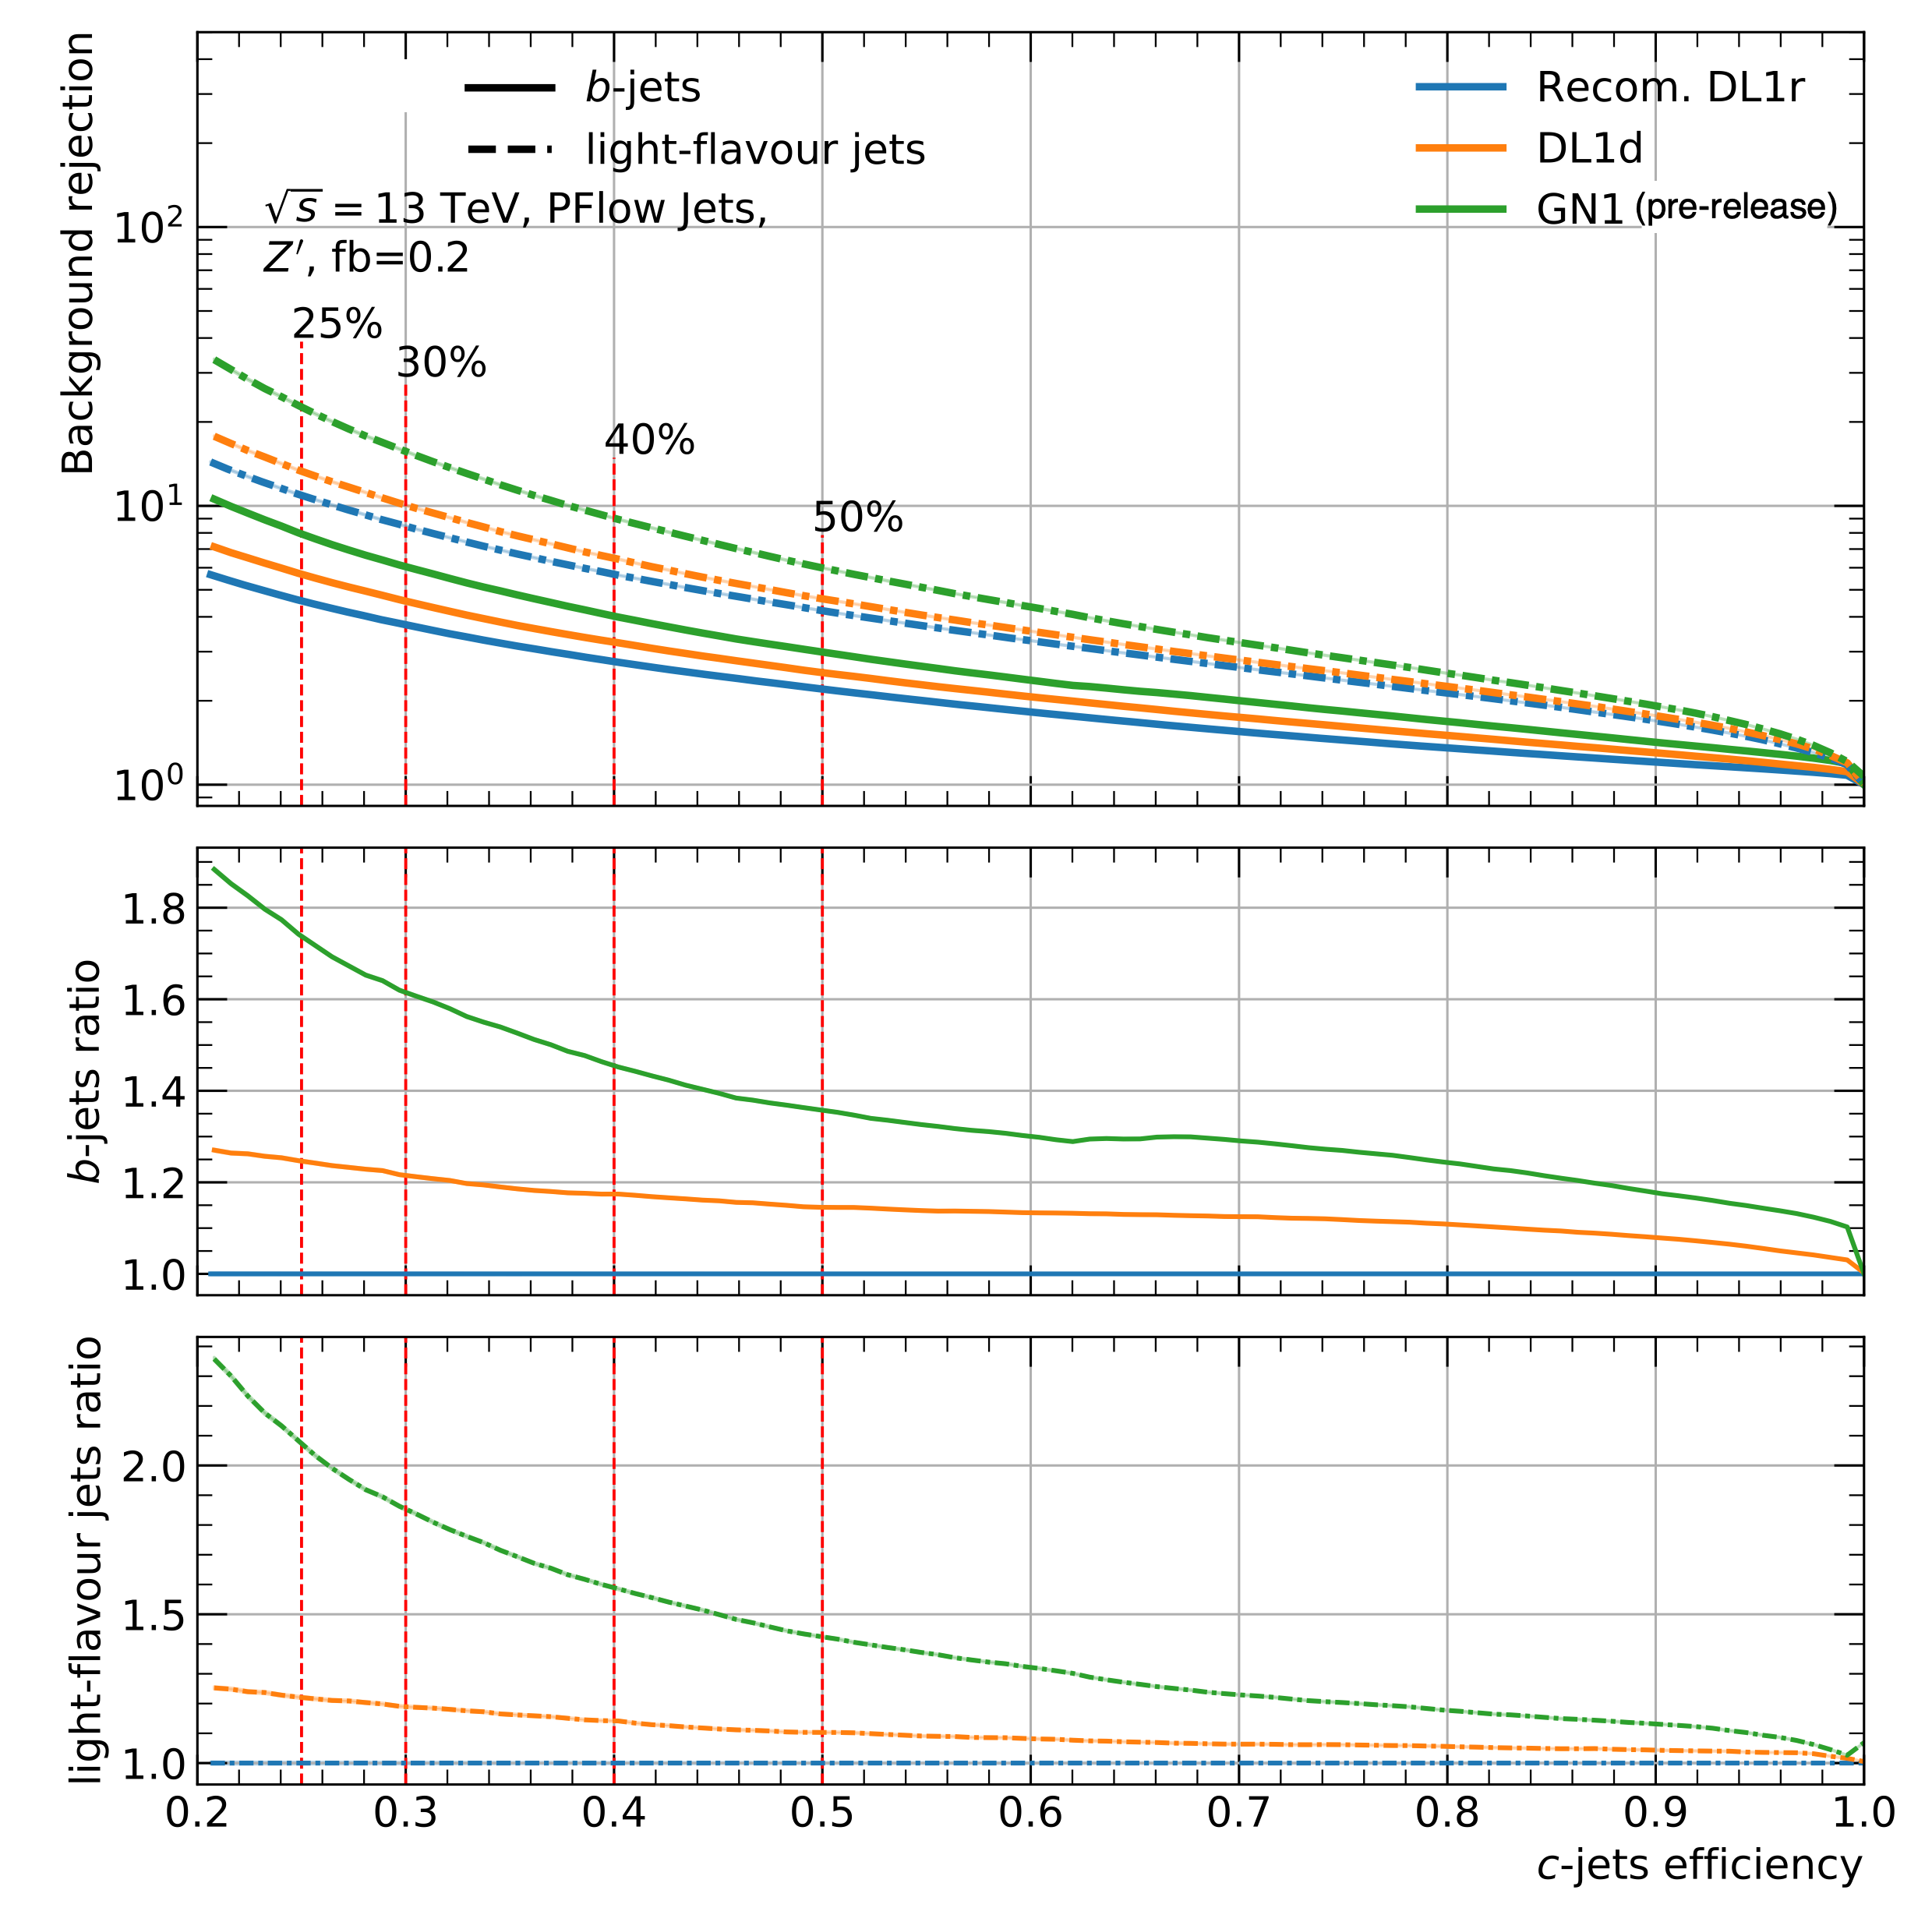
\includegraphics[scale=0.45]{Images/FTAG/DL1d/ROC/zpc.png}
}
\caption{Performance for $c$-tagging with a flavour fraction of $f^c_b = 0.2$. Left: $t\bar{t}$; right: $Z'$. Top: \gls{roc} curves; centre: ratio of $b$-jets rejection from $c$-jets relative to the R22-retrained \gls{dl1r}; bottom: same ratio for light-jets rejection. List of taggers: {\color{blue} recommended \gls{dl1r} from the previous release}; {\color{orange} \gls{dl1d} trained on the new release}; {\color{greenforest} \gls{gn1} test-model trained on the new release}.}
\label{fig:DL1dz}
\end{figure}
\end{center}

\begin{table}[h]
  \begin{center}
      \begin{tabular}{C{2cm}|cc} 
      	 \hline \hline
          \multicolumn{3}{c}{$b$-tagging on $t\bar{t}$} \\ \hline
          WP & $c$-rejection  & light-rejection  \\ \hline
          60\%   & +26\% & +73\% \\ 
          70\%   & +19\% & +56\% \\ 
          77\%   & +12\% & +41\% \\ 
          85\%   & +7\%   & +32\% \\ \hline
          \multicolumn{3}{c}{} \\
           \hline  \hline
           \multicolumn{3}{c}{$c$-tagging on $t\bar{t}$} \\ \hline
          WP & $b$-rejection  & light-rejection  \\ \hline
          25\%   & +26\% & +5\% \\
          30\%   & +25\% & +9\% \\
          40\%   & +22\% & +12\% \\
          50\%   & +18\% & +15\% \\ \hline \hline
      \end{tabular}
      \quad
       \begin{tabular}{C{2cm}|cc} 
       	 \hline  \hline
          \multicolumn{3}{c}{$b$-tagging on $Z'$} \\ \hline
          WP & $c$-rejection  & light-rejection  \\ \hline
          60\%   & +19\% & +43\% \\
          70\%   & +10\% & +32\% \\
          77\%   & +9\%  & +26\% \\
          85\%   & +6\%  & +19\% \\ \hline
          \multicolumn{3}{c}{} \\
           \hline  \hline
           \multicolumn{3}{c}{$c$-tagging on $Z'$} \\ \hline
          WP & $b$-rejection  & light-rejection  \\ \hline
          25\%   & +12\% & +22\% \\
          30\%   & +11\% & +19\% \\
          40\%   & +8\%   & +14\% \\
          50\%   & +7\%   & +10\% \\ \hline  \hline
      \end{tabular}
    \caption{The change in background flavour rejection of \gls{dl1d} relative to \gls{dl1r} at various tagging efficiencies, both trained on the new release. Top: $b$-tagging ($f^b_c = 0.018$); bottom: $c$-tagging ($f^c_b = 0.2$); left: $t\bar{t}$; right: $Z'$.}
    \label{tab:max-perf}
  \end{center}
\end{table}

%
\begin{center}
\begin{figure}[h!]
%\vspace{-0.2cm}
\centerline{
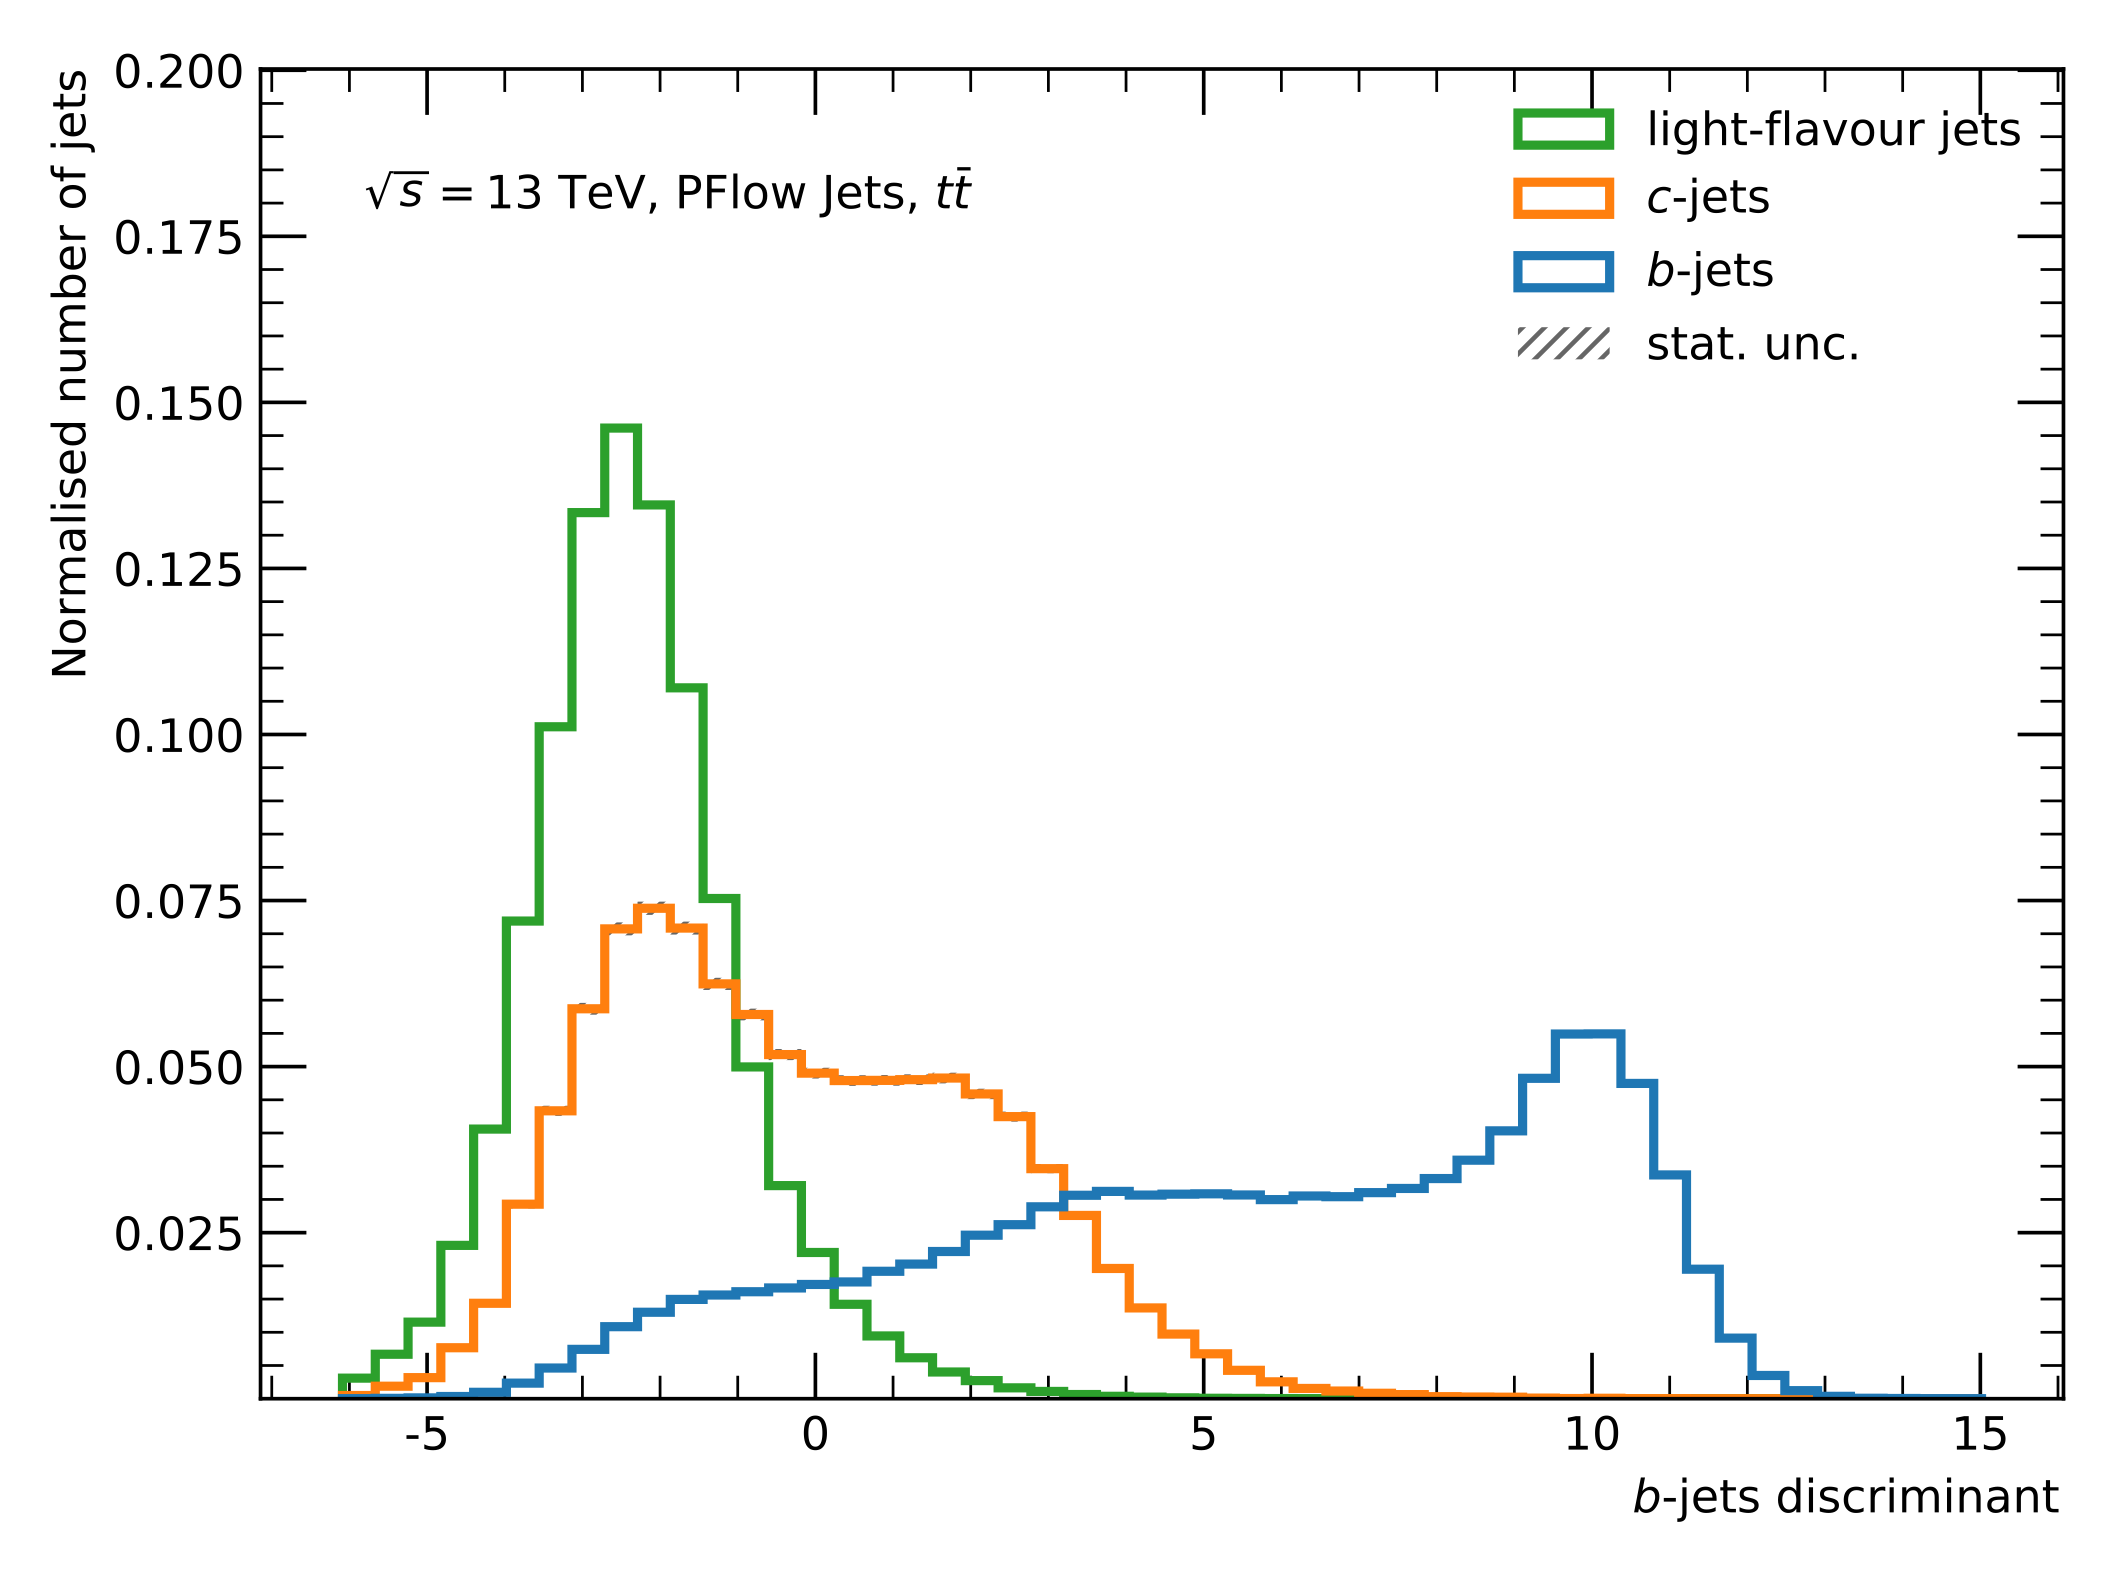
\includegraphics[scale=0.5]{Images/FTAG/DL1d/ROC/scores_DL1_ttbar_300.png}
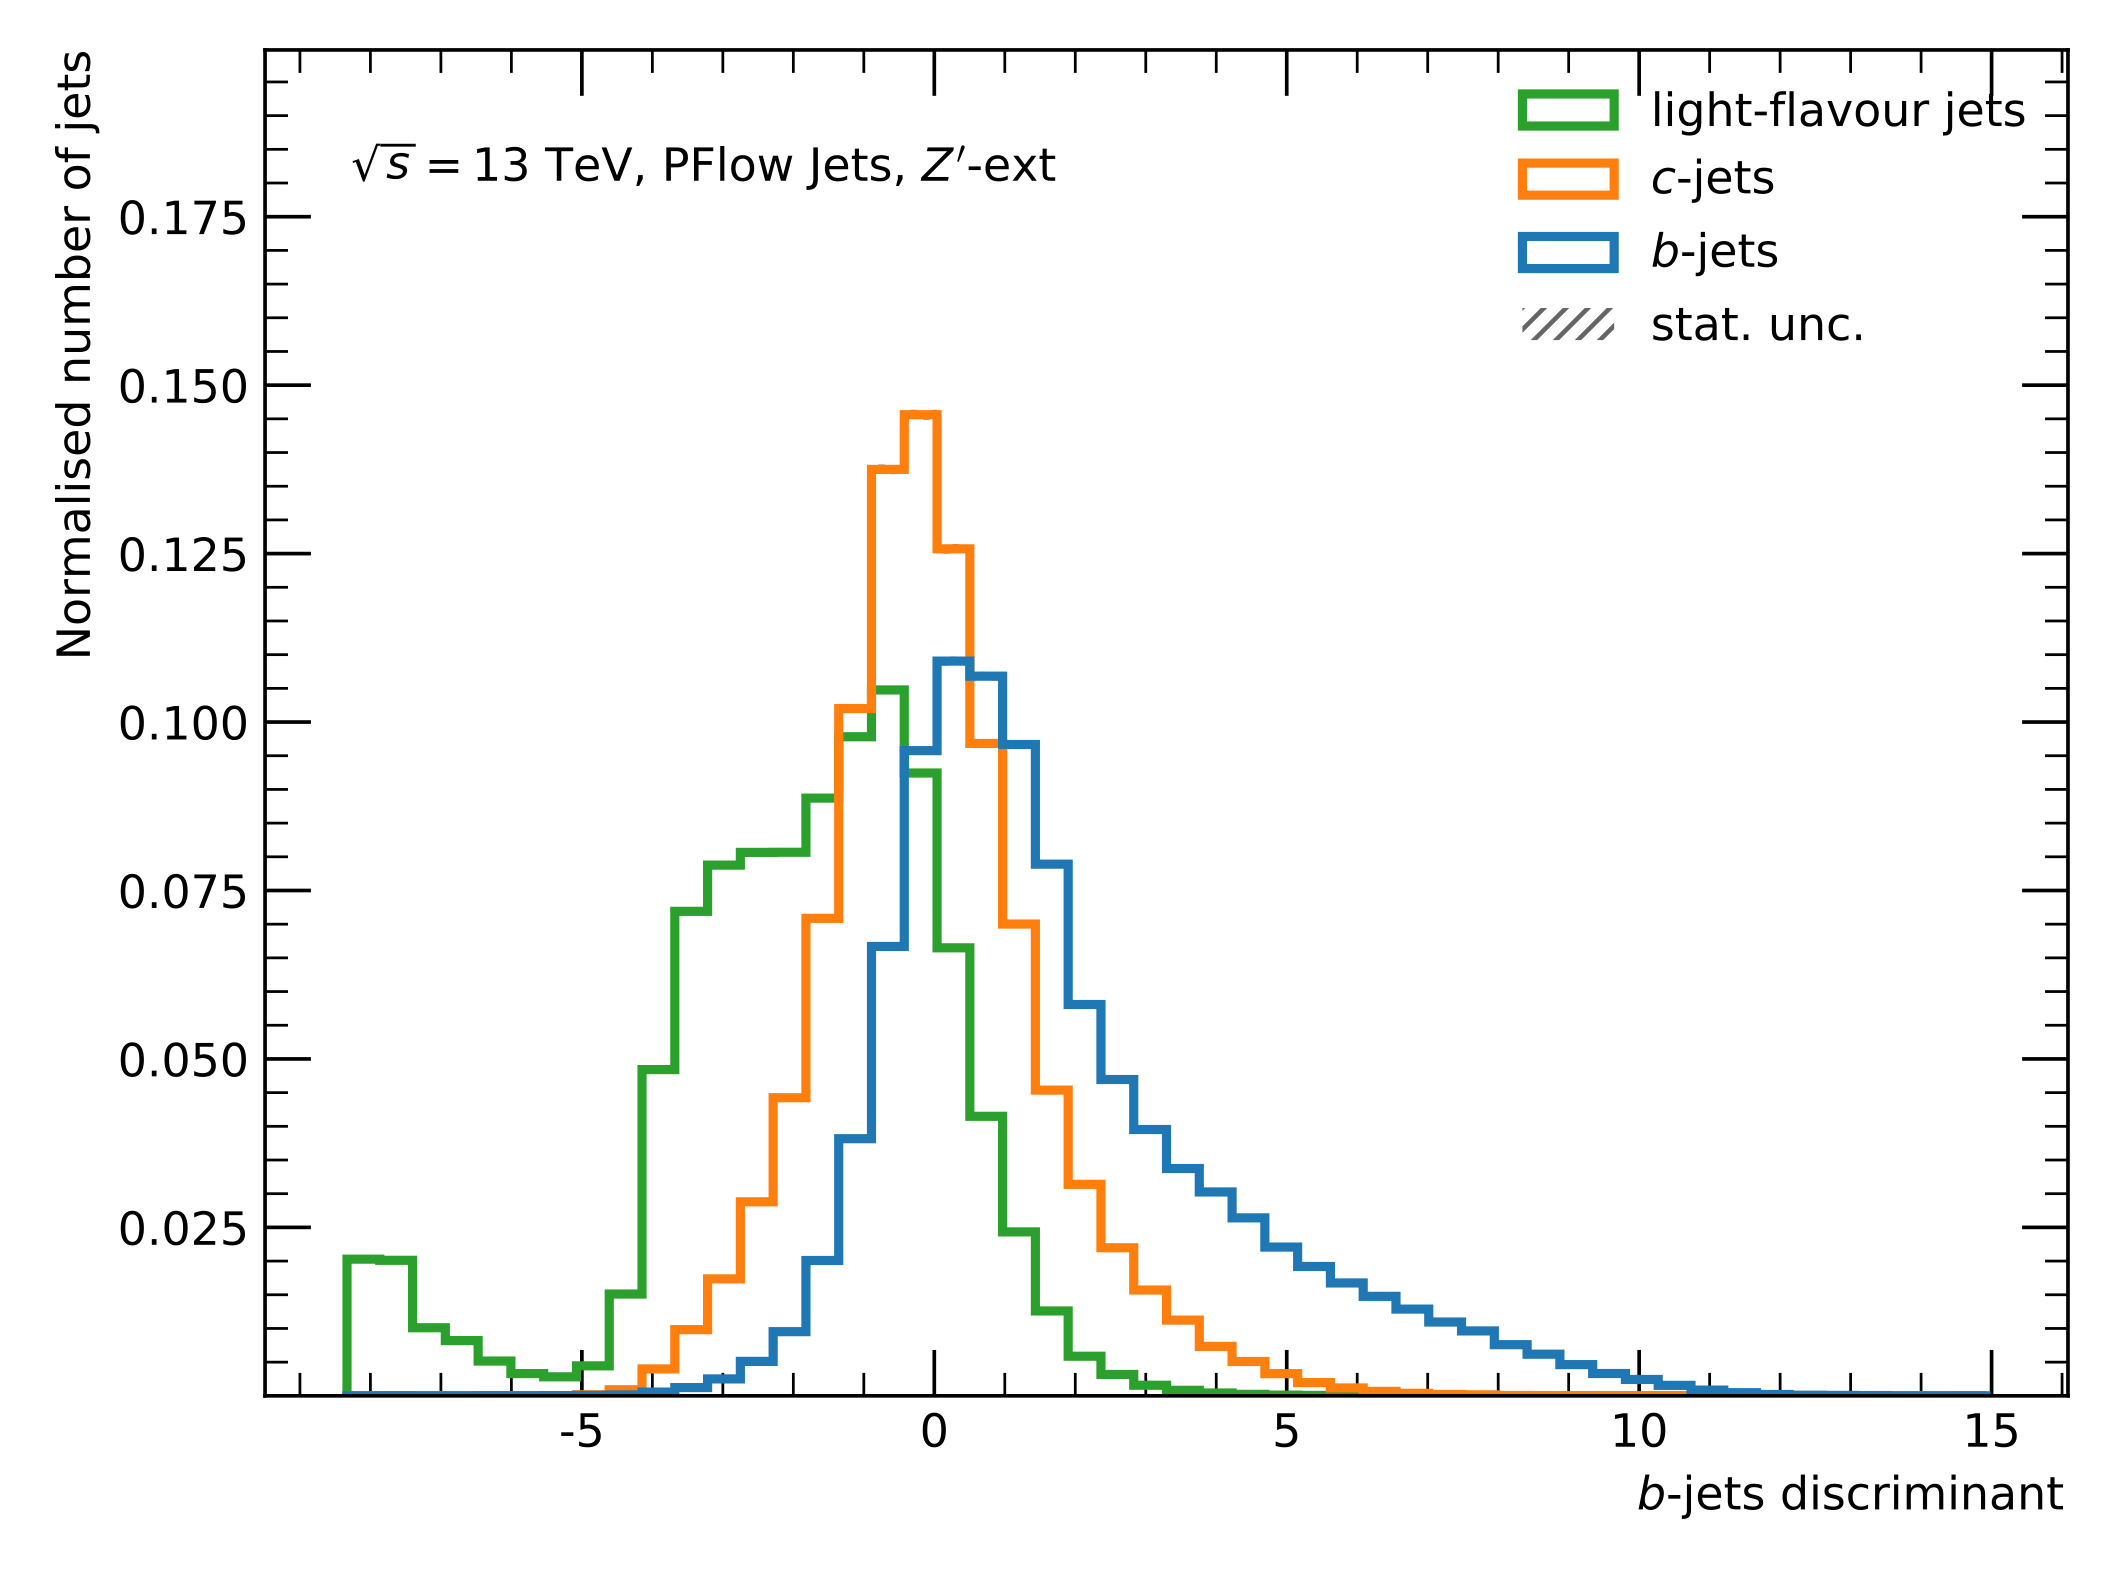
\includegraphics[scale=0.5]{Images/FTAG/DL1d/ROC/scores_DL1_zp_300.png}
}
\caption{Distribution of \gls{dl1d} $b$-tagging discriminant with $f_c = 0.018$ for the different jet flavours, evaluated on $t\bar{t}$ (left) and $Z'$ (right).}
\label{fig:scoreDL1dtt}
\centerline{
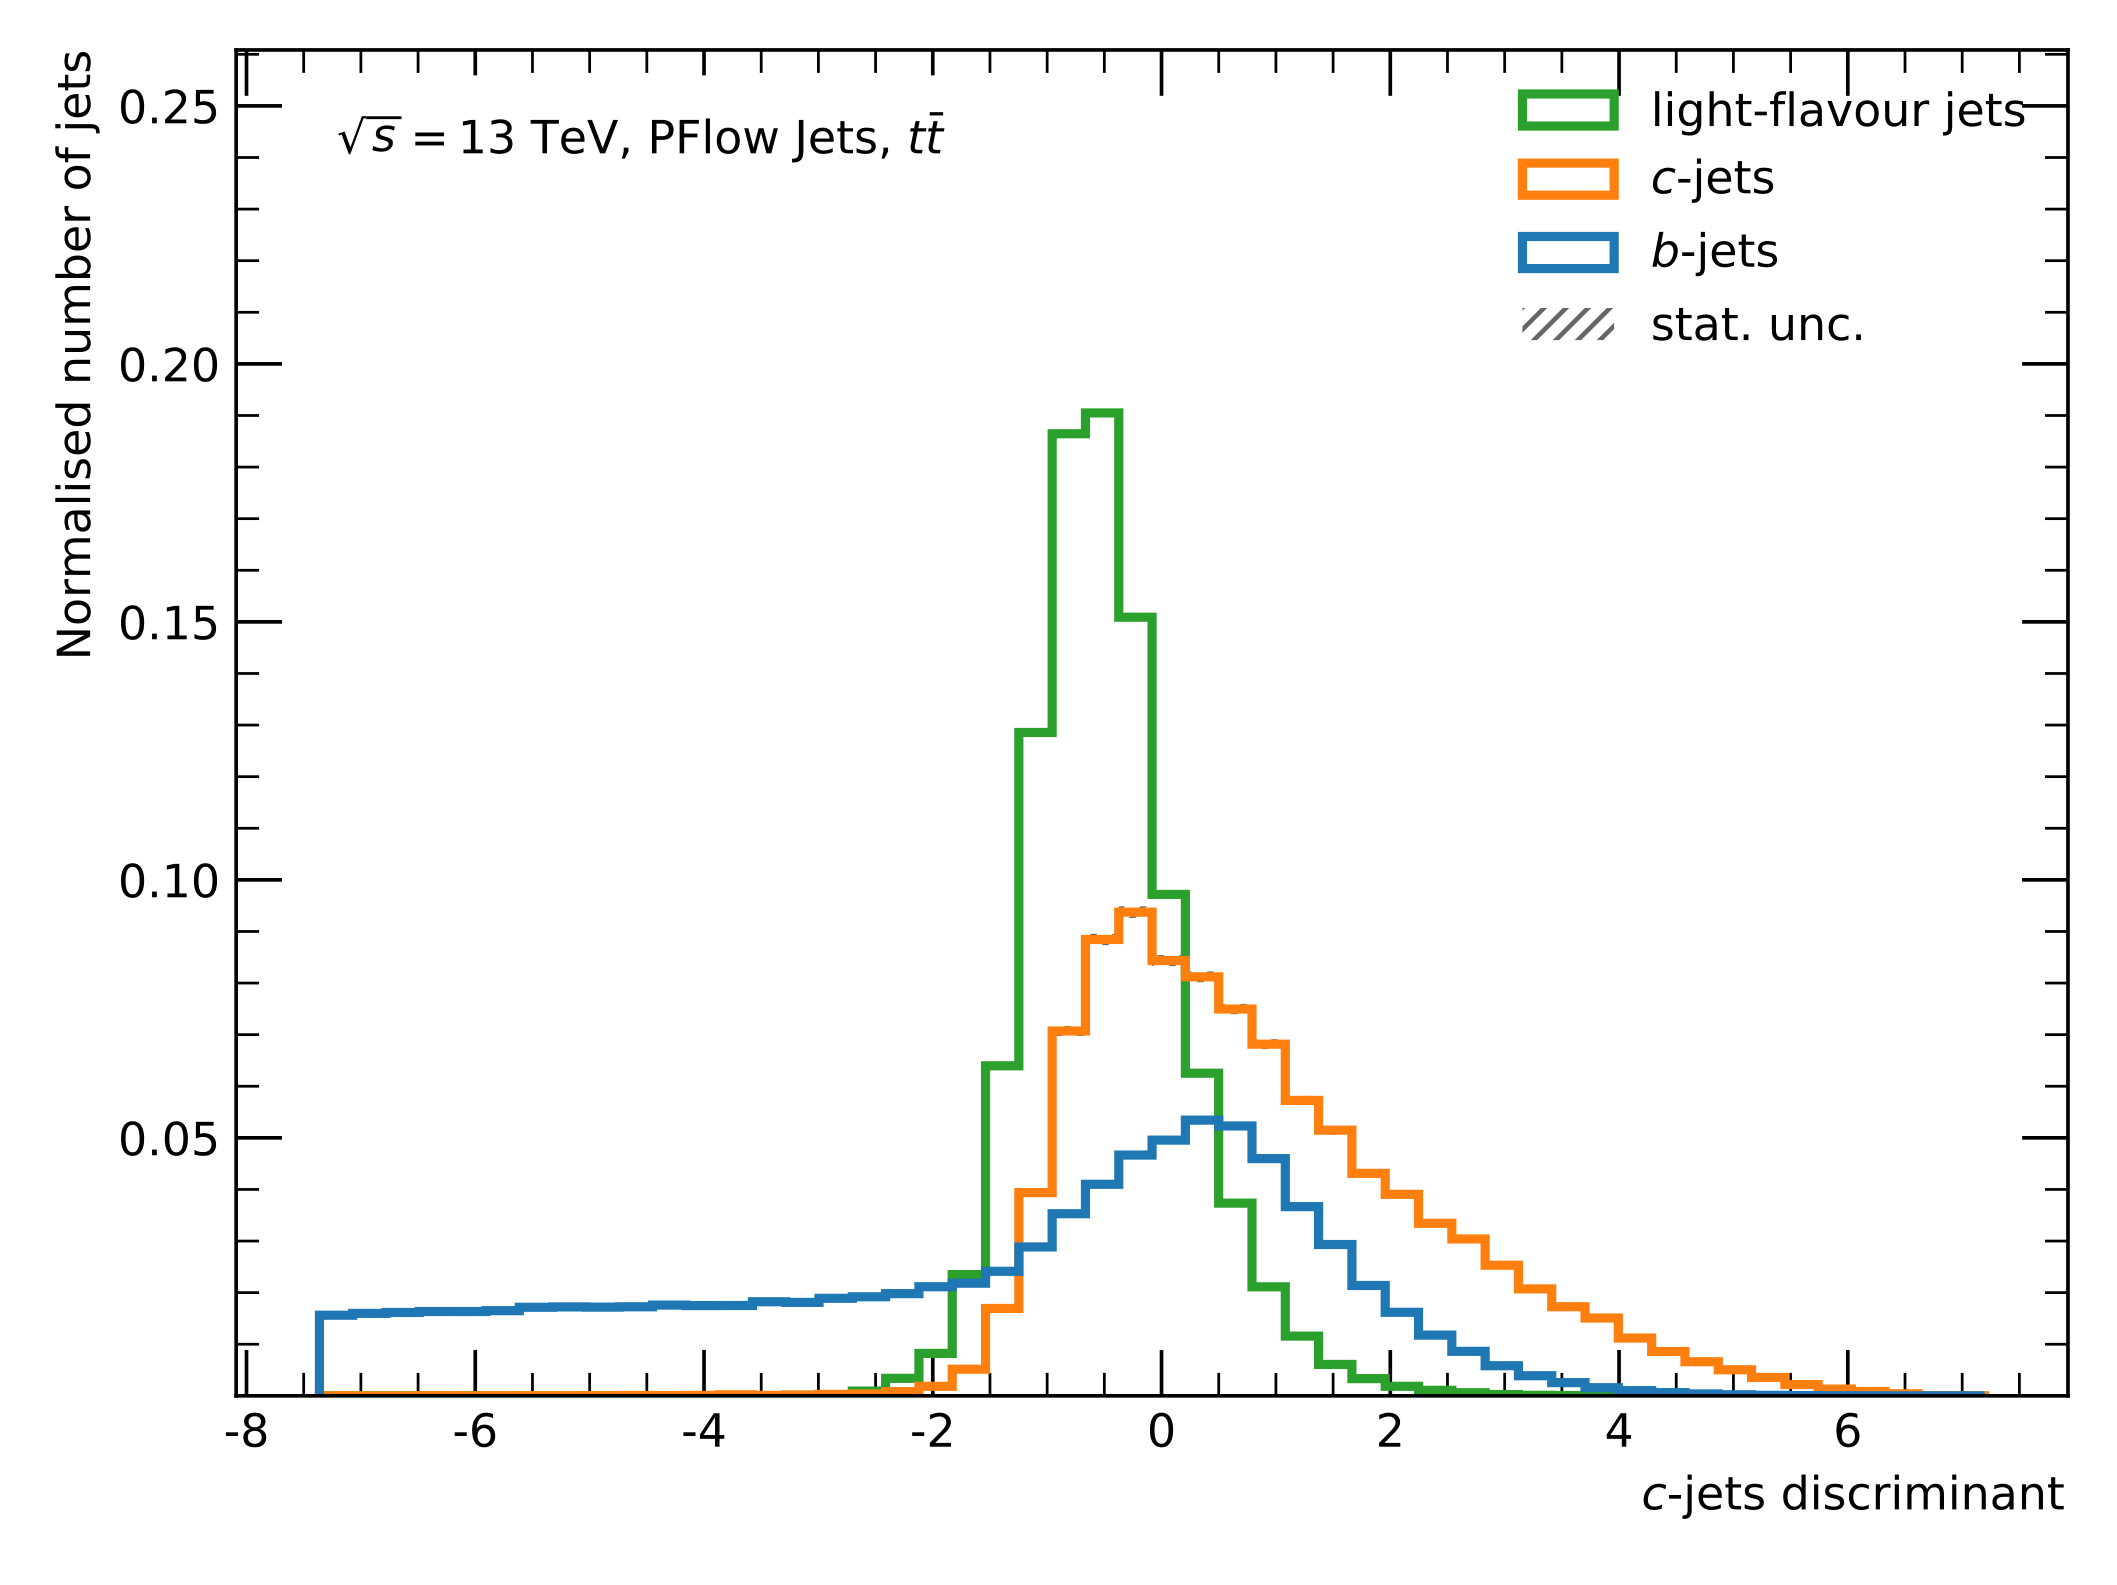
\includegraphics[scale=0.5]{Images/FTAG/DL1d/ROC/scores_DL1_ttbar_c_299.png}
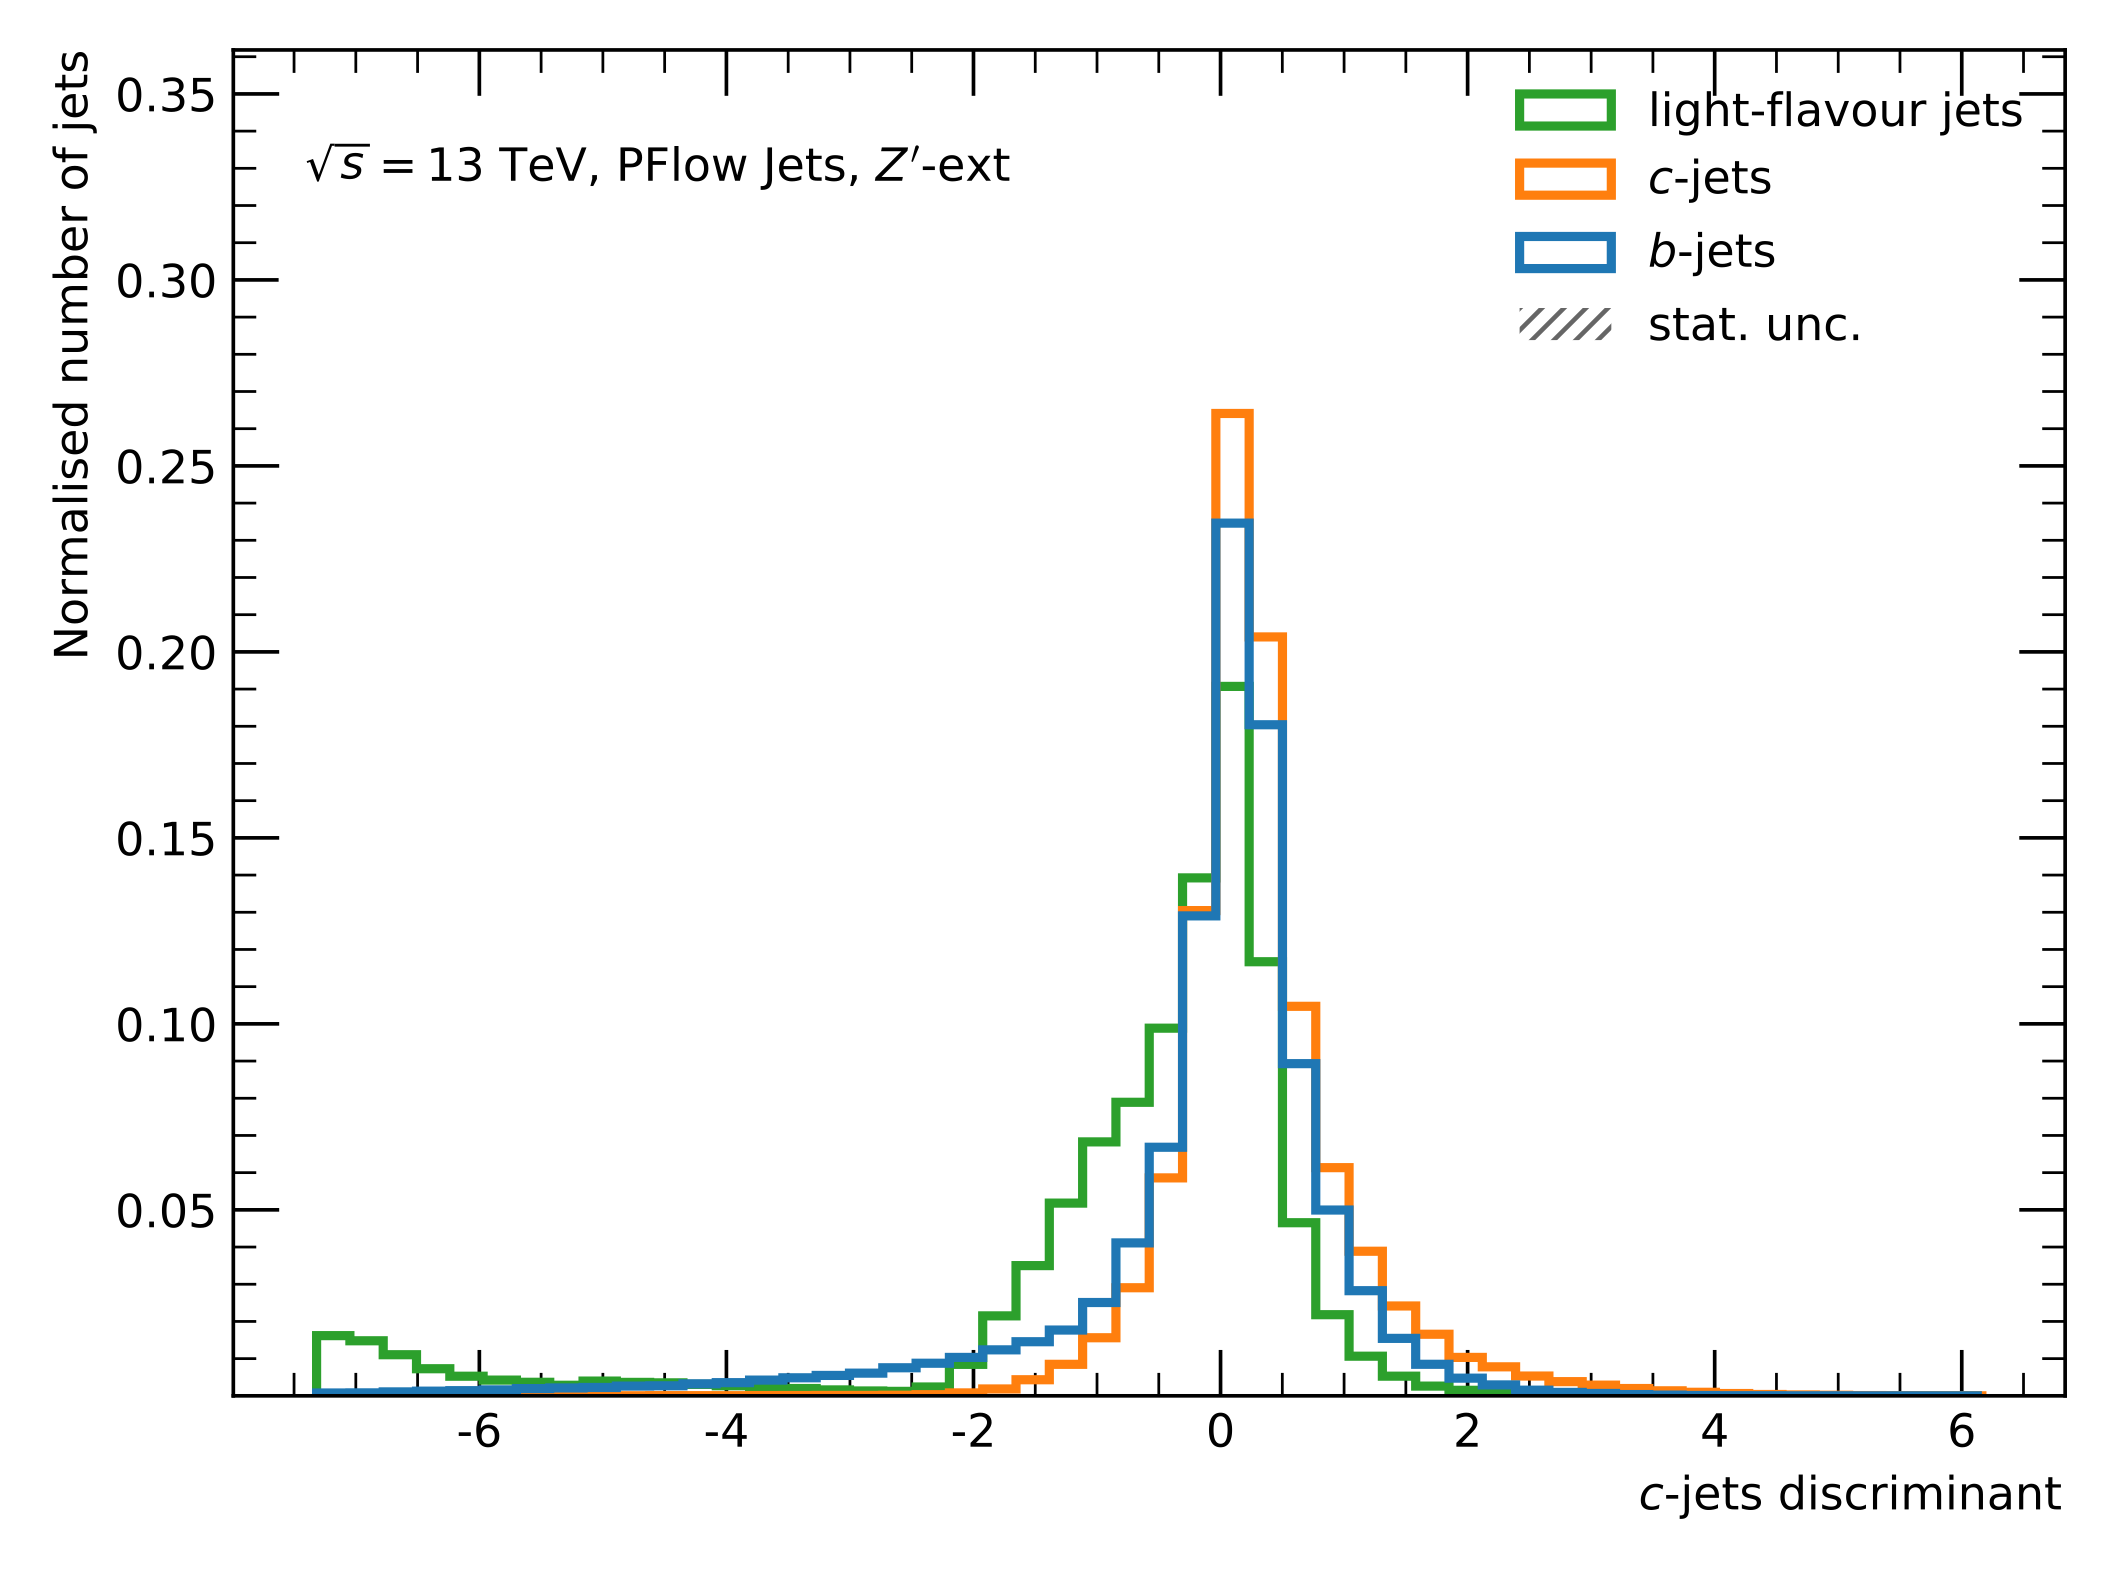
\includegraphics[scale=0.5]{Images/FTAG/DL1d/ROC/scores_DL1_zp_c_299.png}
}
%\vspace{-0.3cm}
\caption{Distribution of \gls{dl1d} $c$-tagging discriminant with $f_b = 0.2$ for the different jet flavours, evaluated on $t\bar{t}$ (left) and $Z'$ (right).}
\label{fig:scoreDL1dz}
\end{figure}
\end{center}
%
\newpage
%
\begin{center}
\begin{figure}[h!]
\vspace{-0.55cm}
\centerline{
  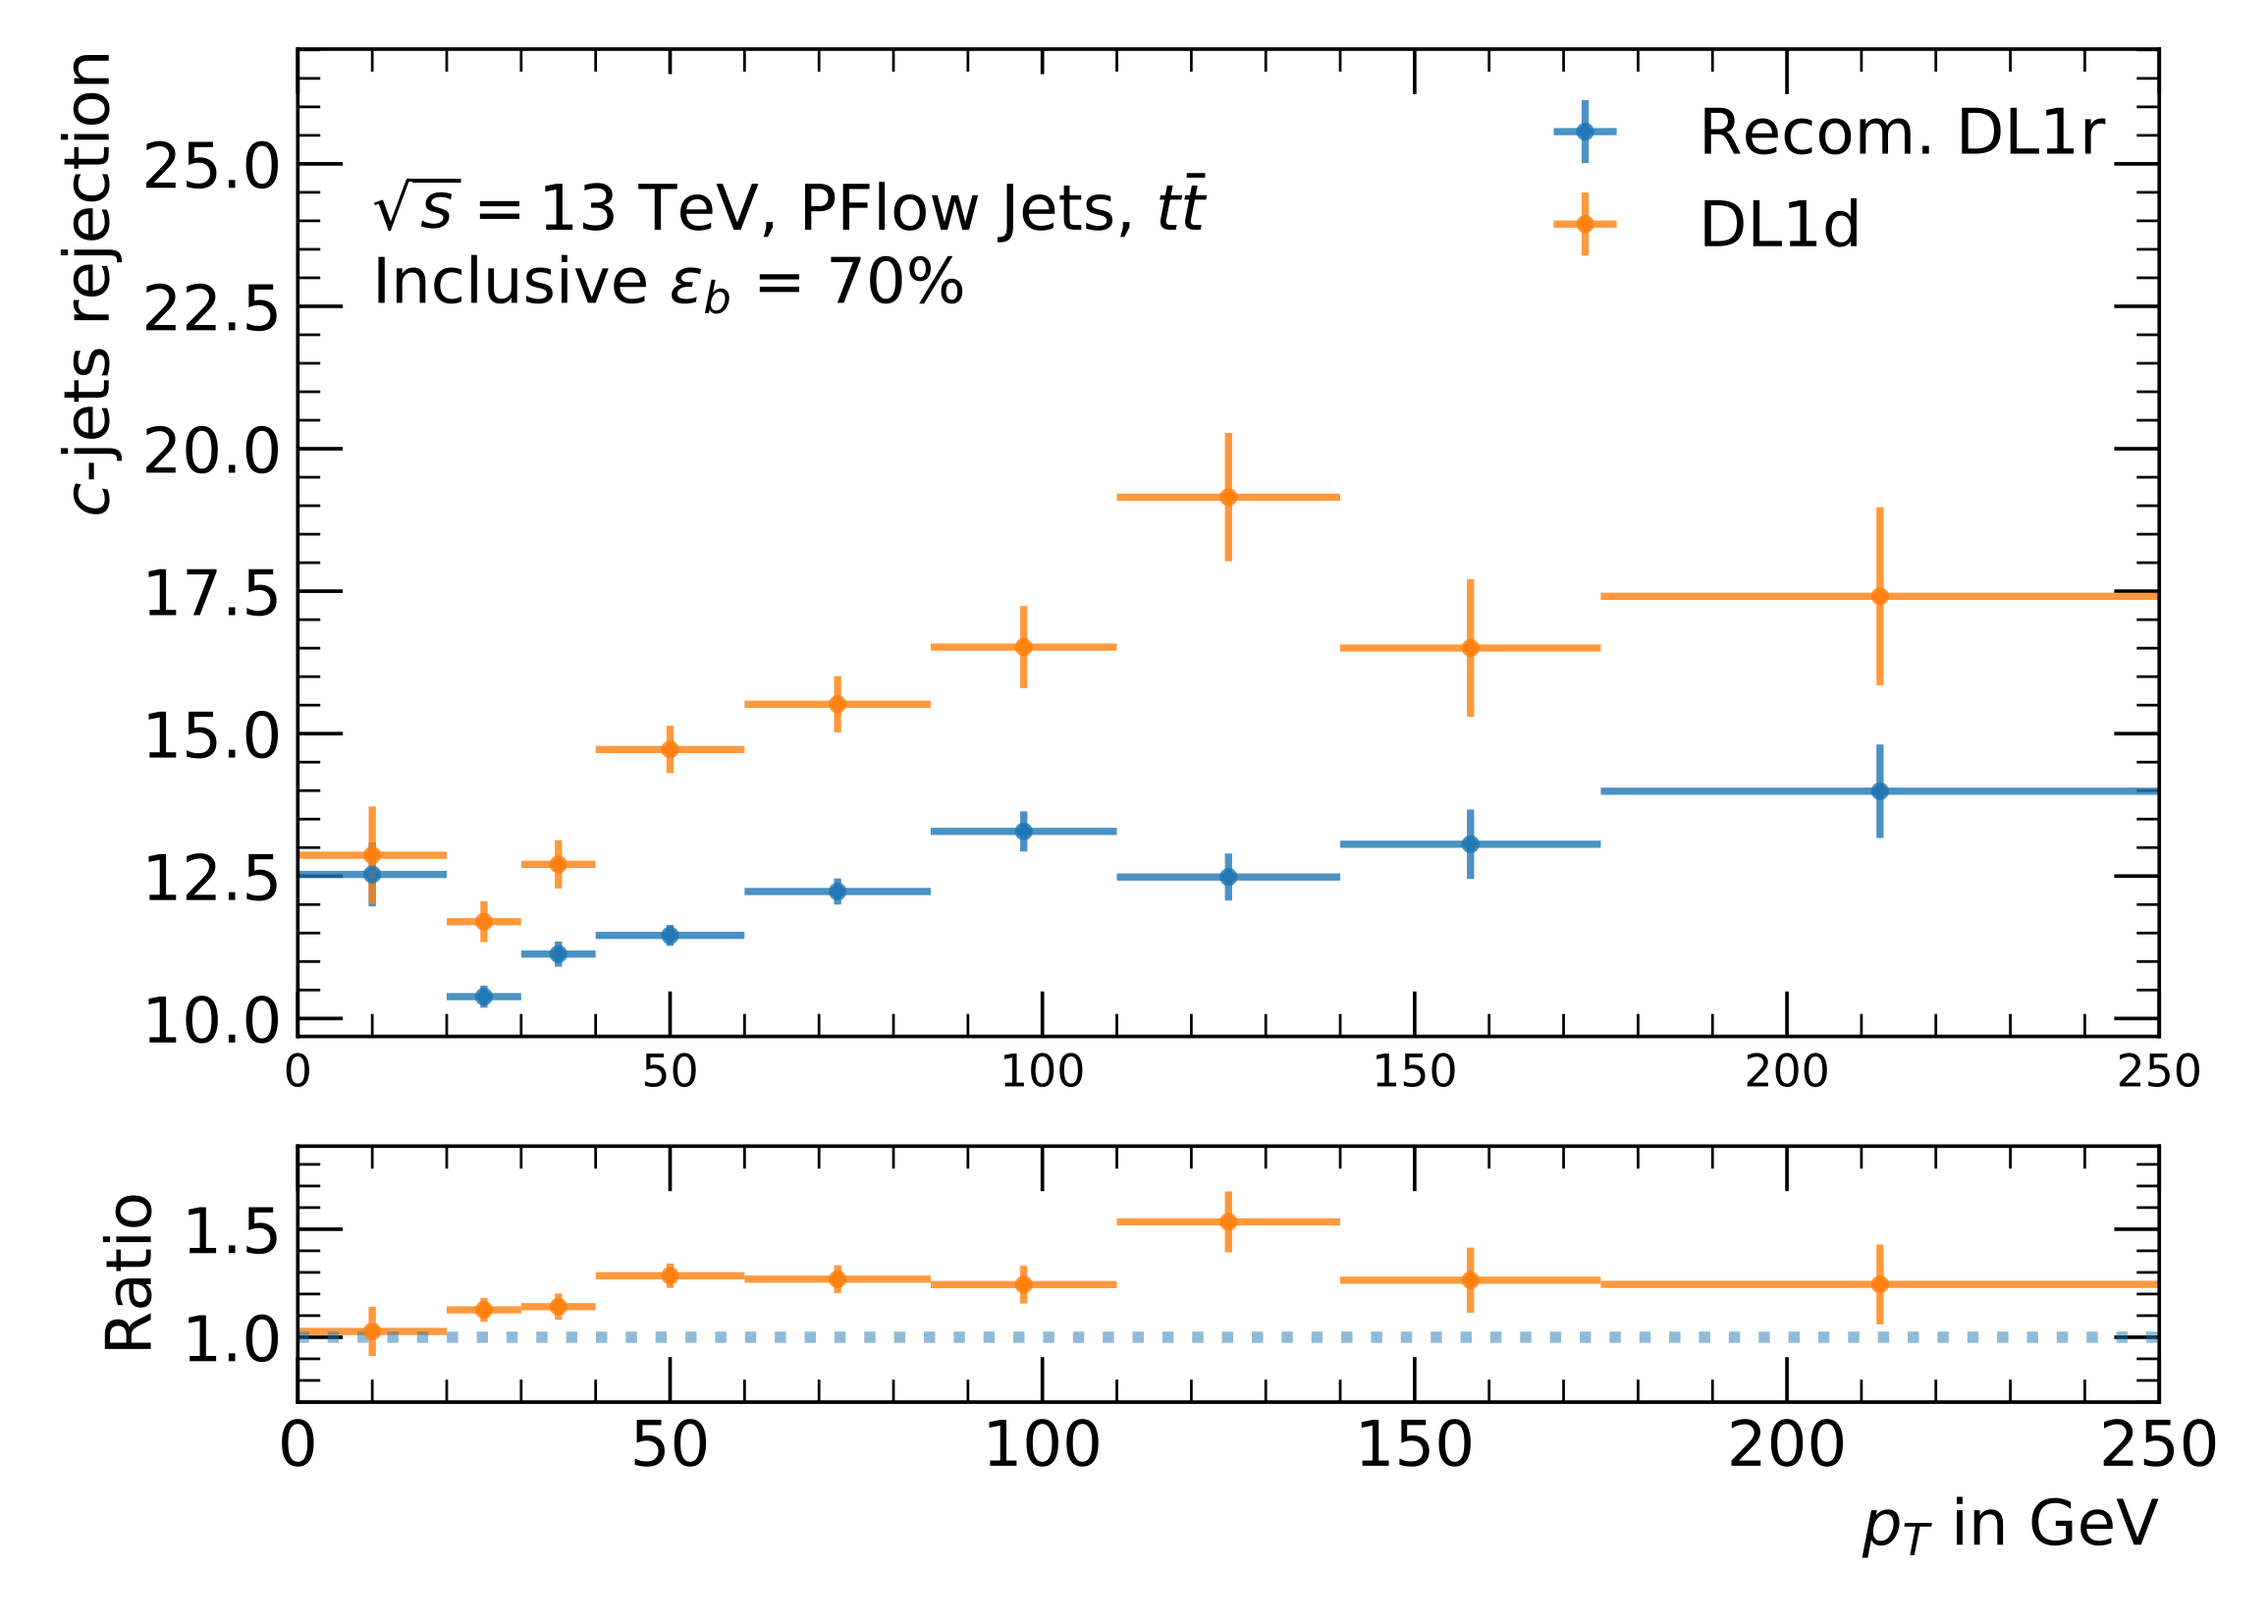
\includegraphics[scale=0.425]{Images/FTAG/DL1d/perpT/ttbc.png}
  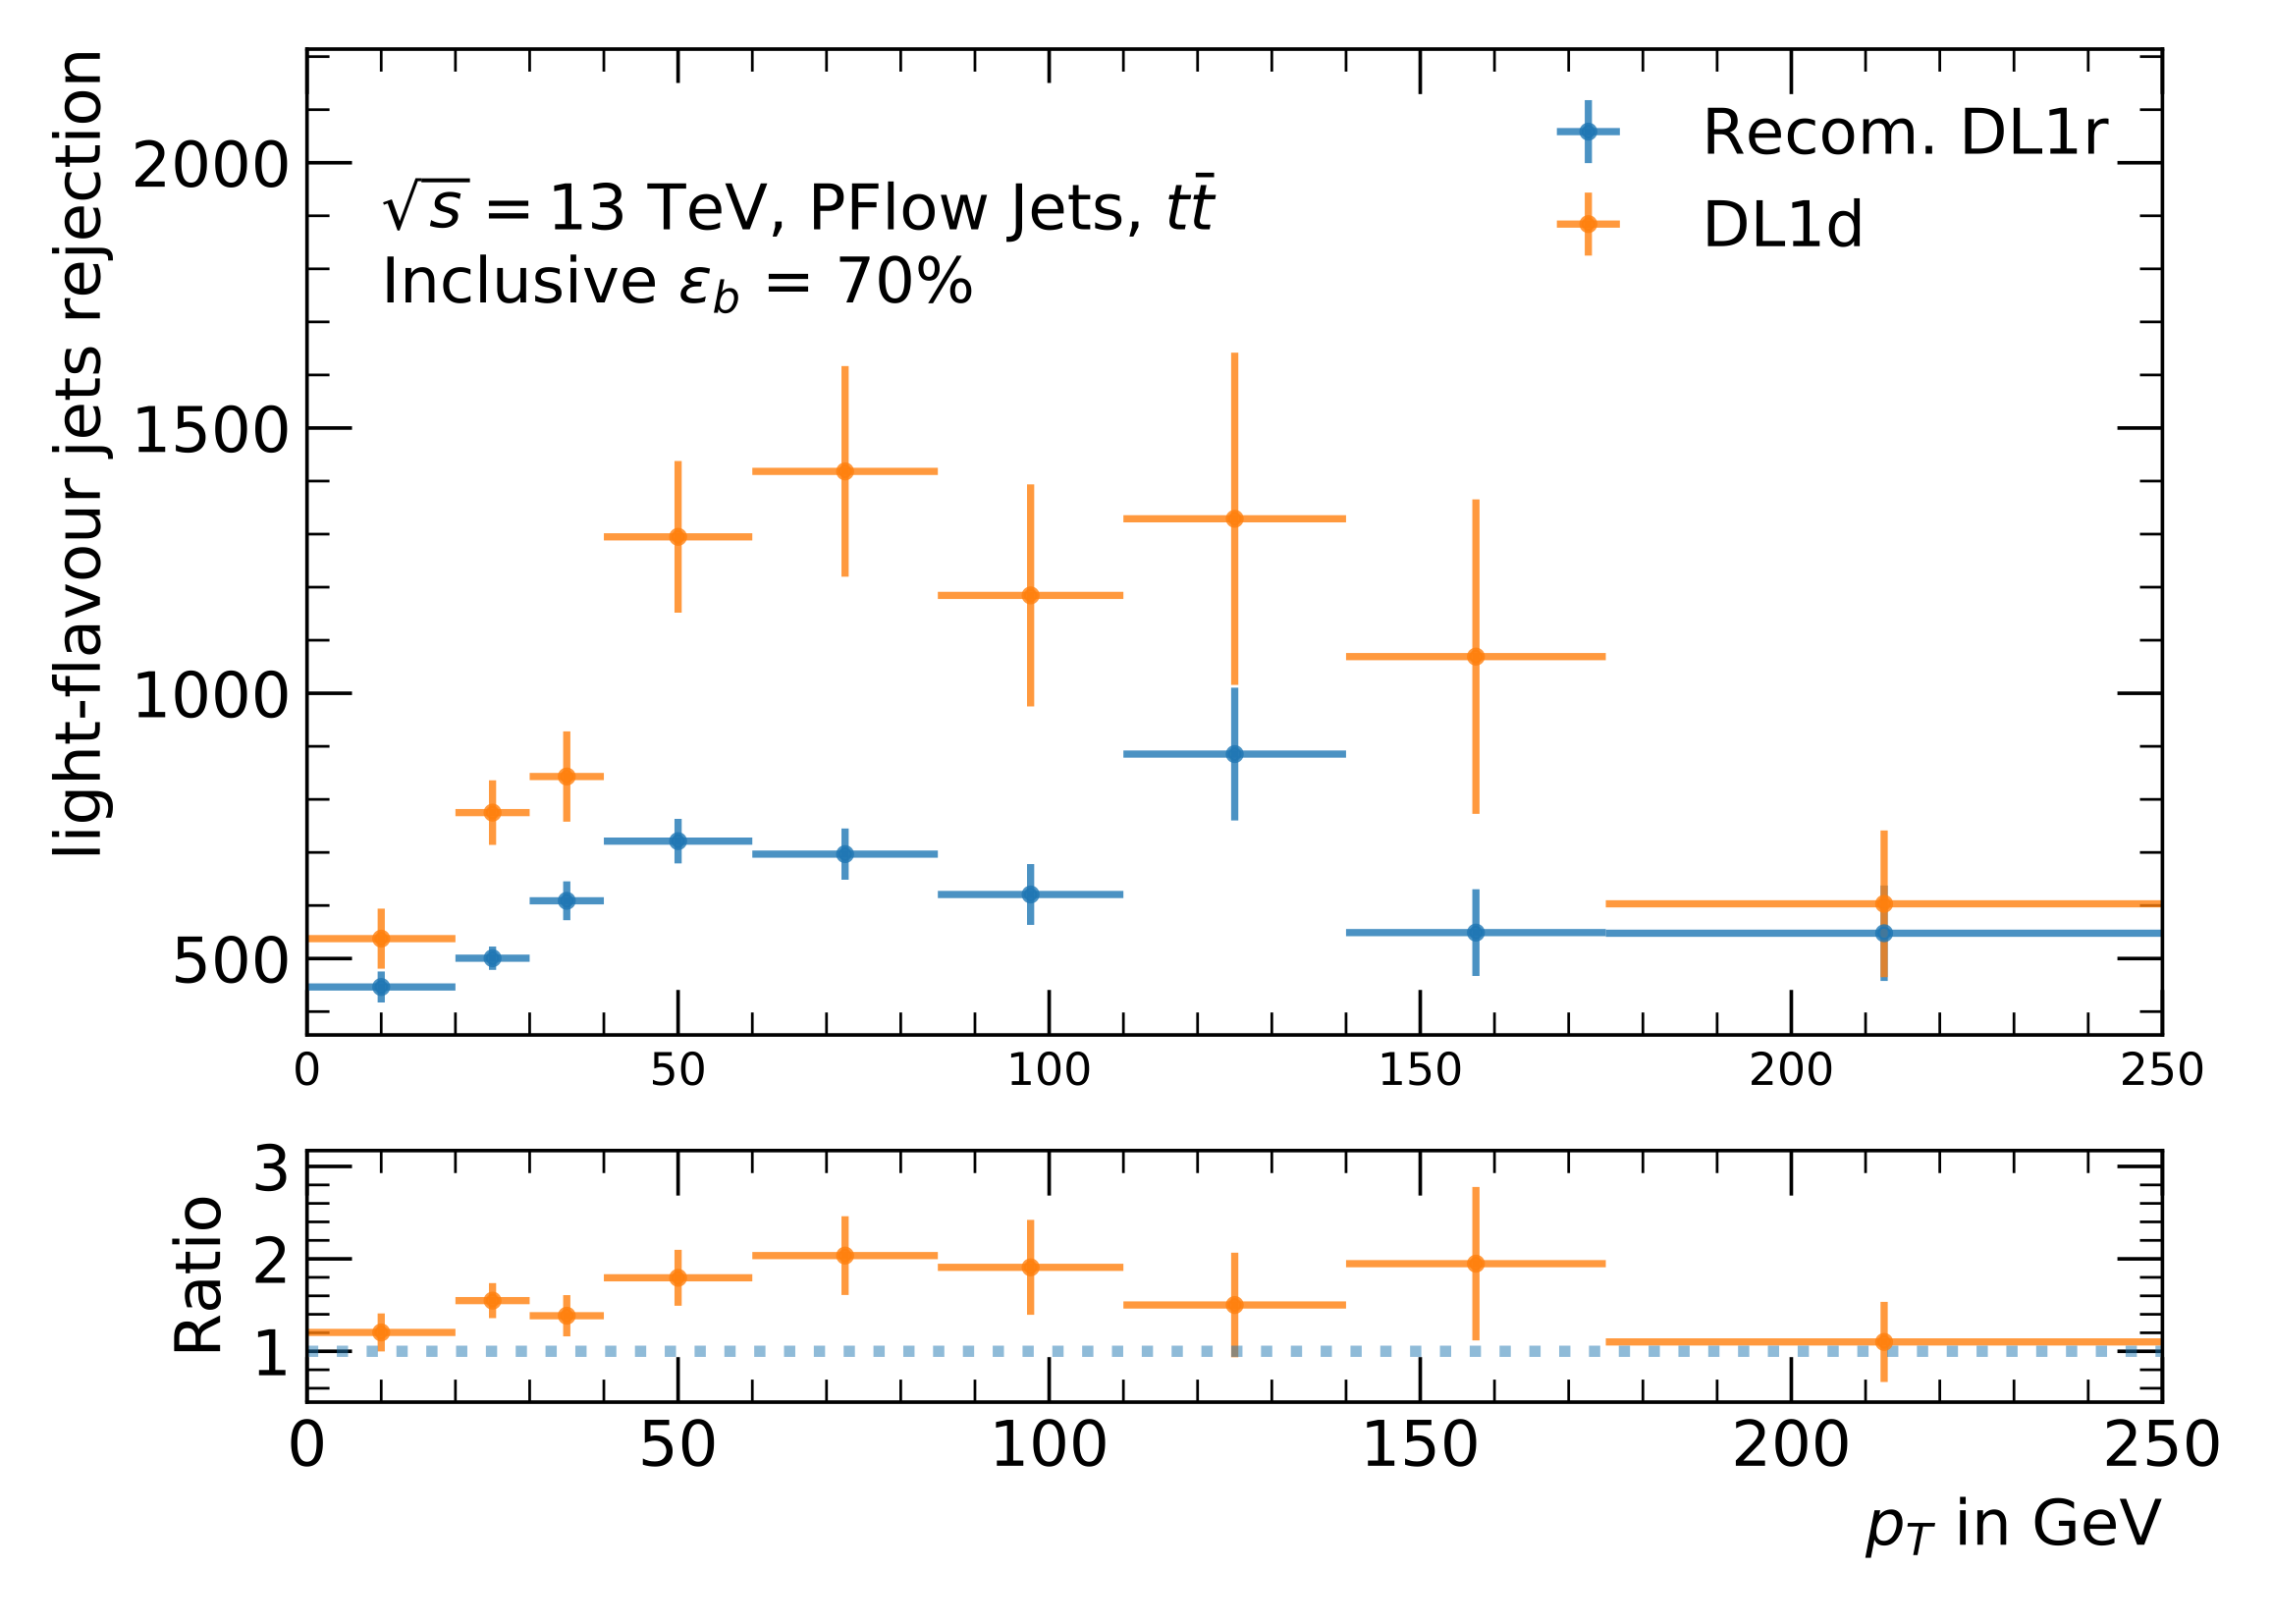
\includegraphics[scale=0.425]{Images/FTAG/DL1d/perpT/ttbu.png}
}
\centerline{
  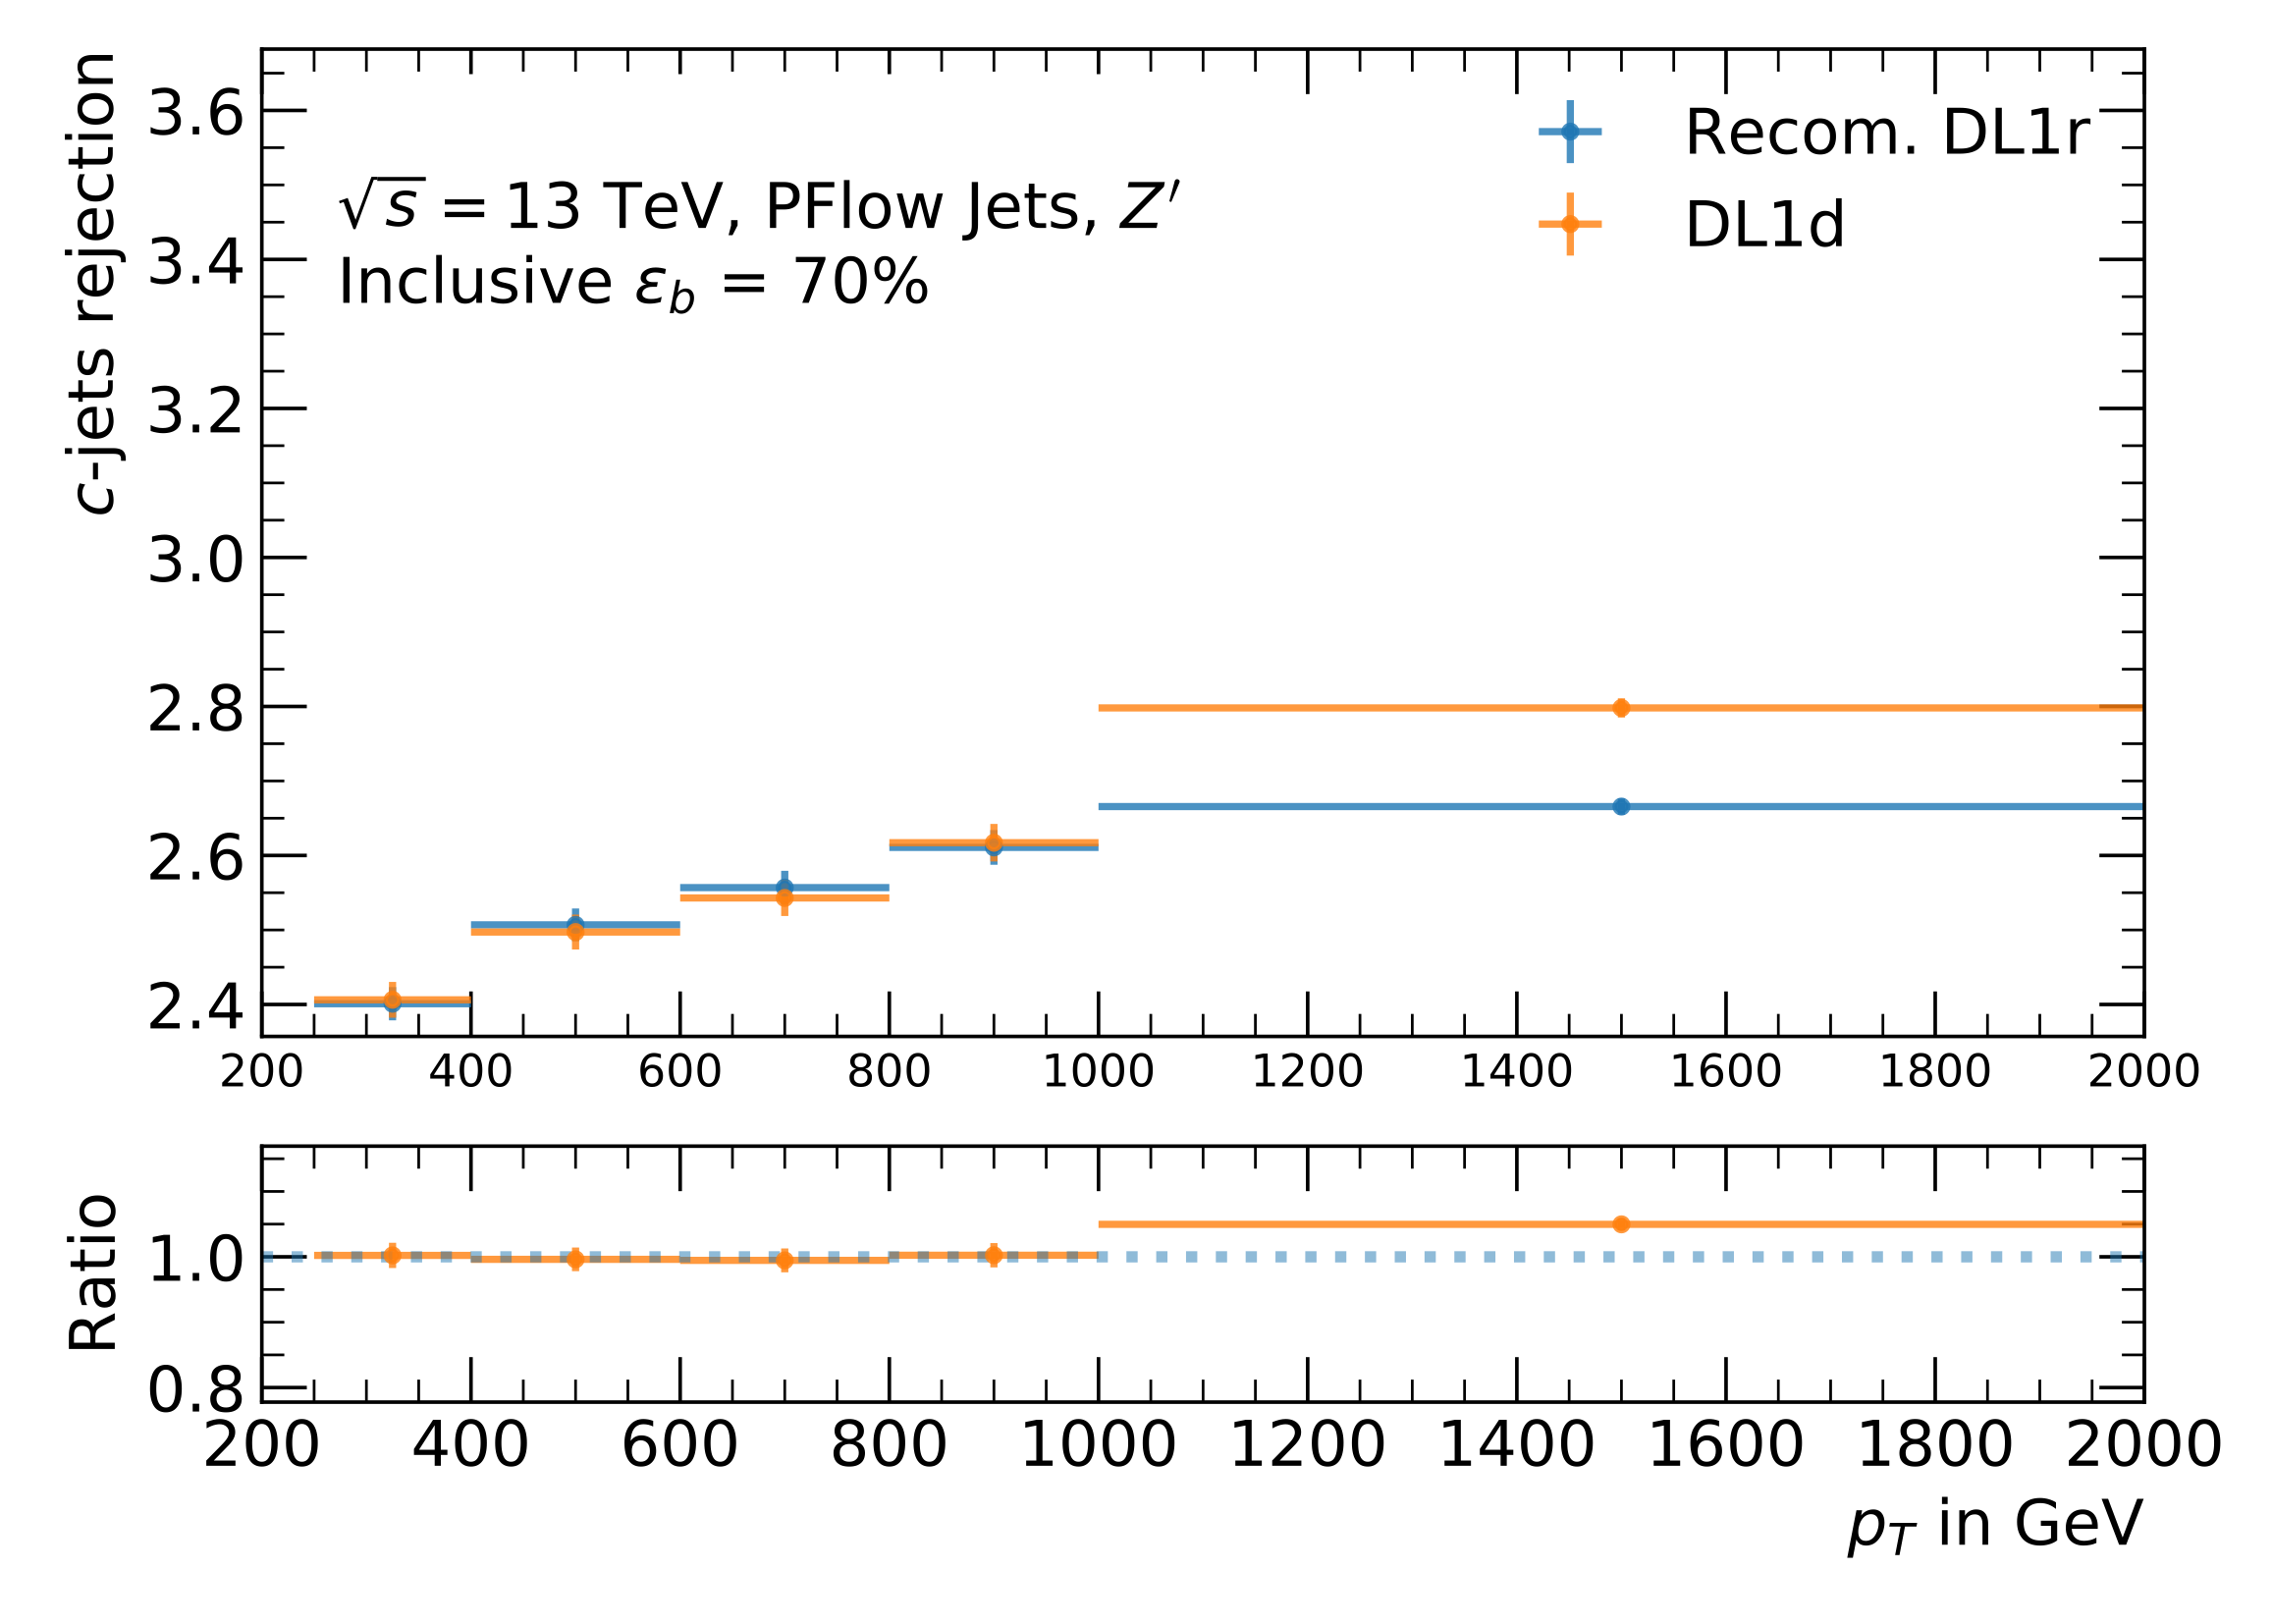
\includegraphics[scale=0.425]{Images/FTAG/DL1d/perpT/zpbc.png}
  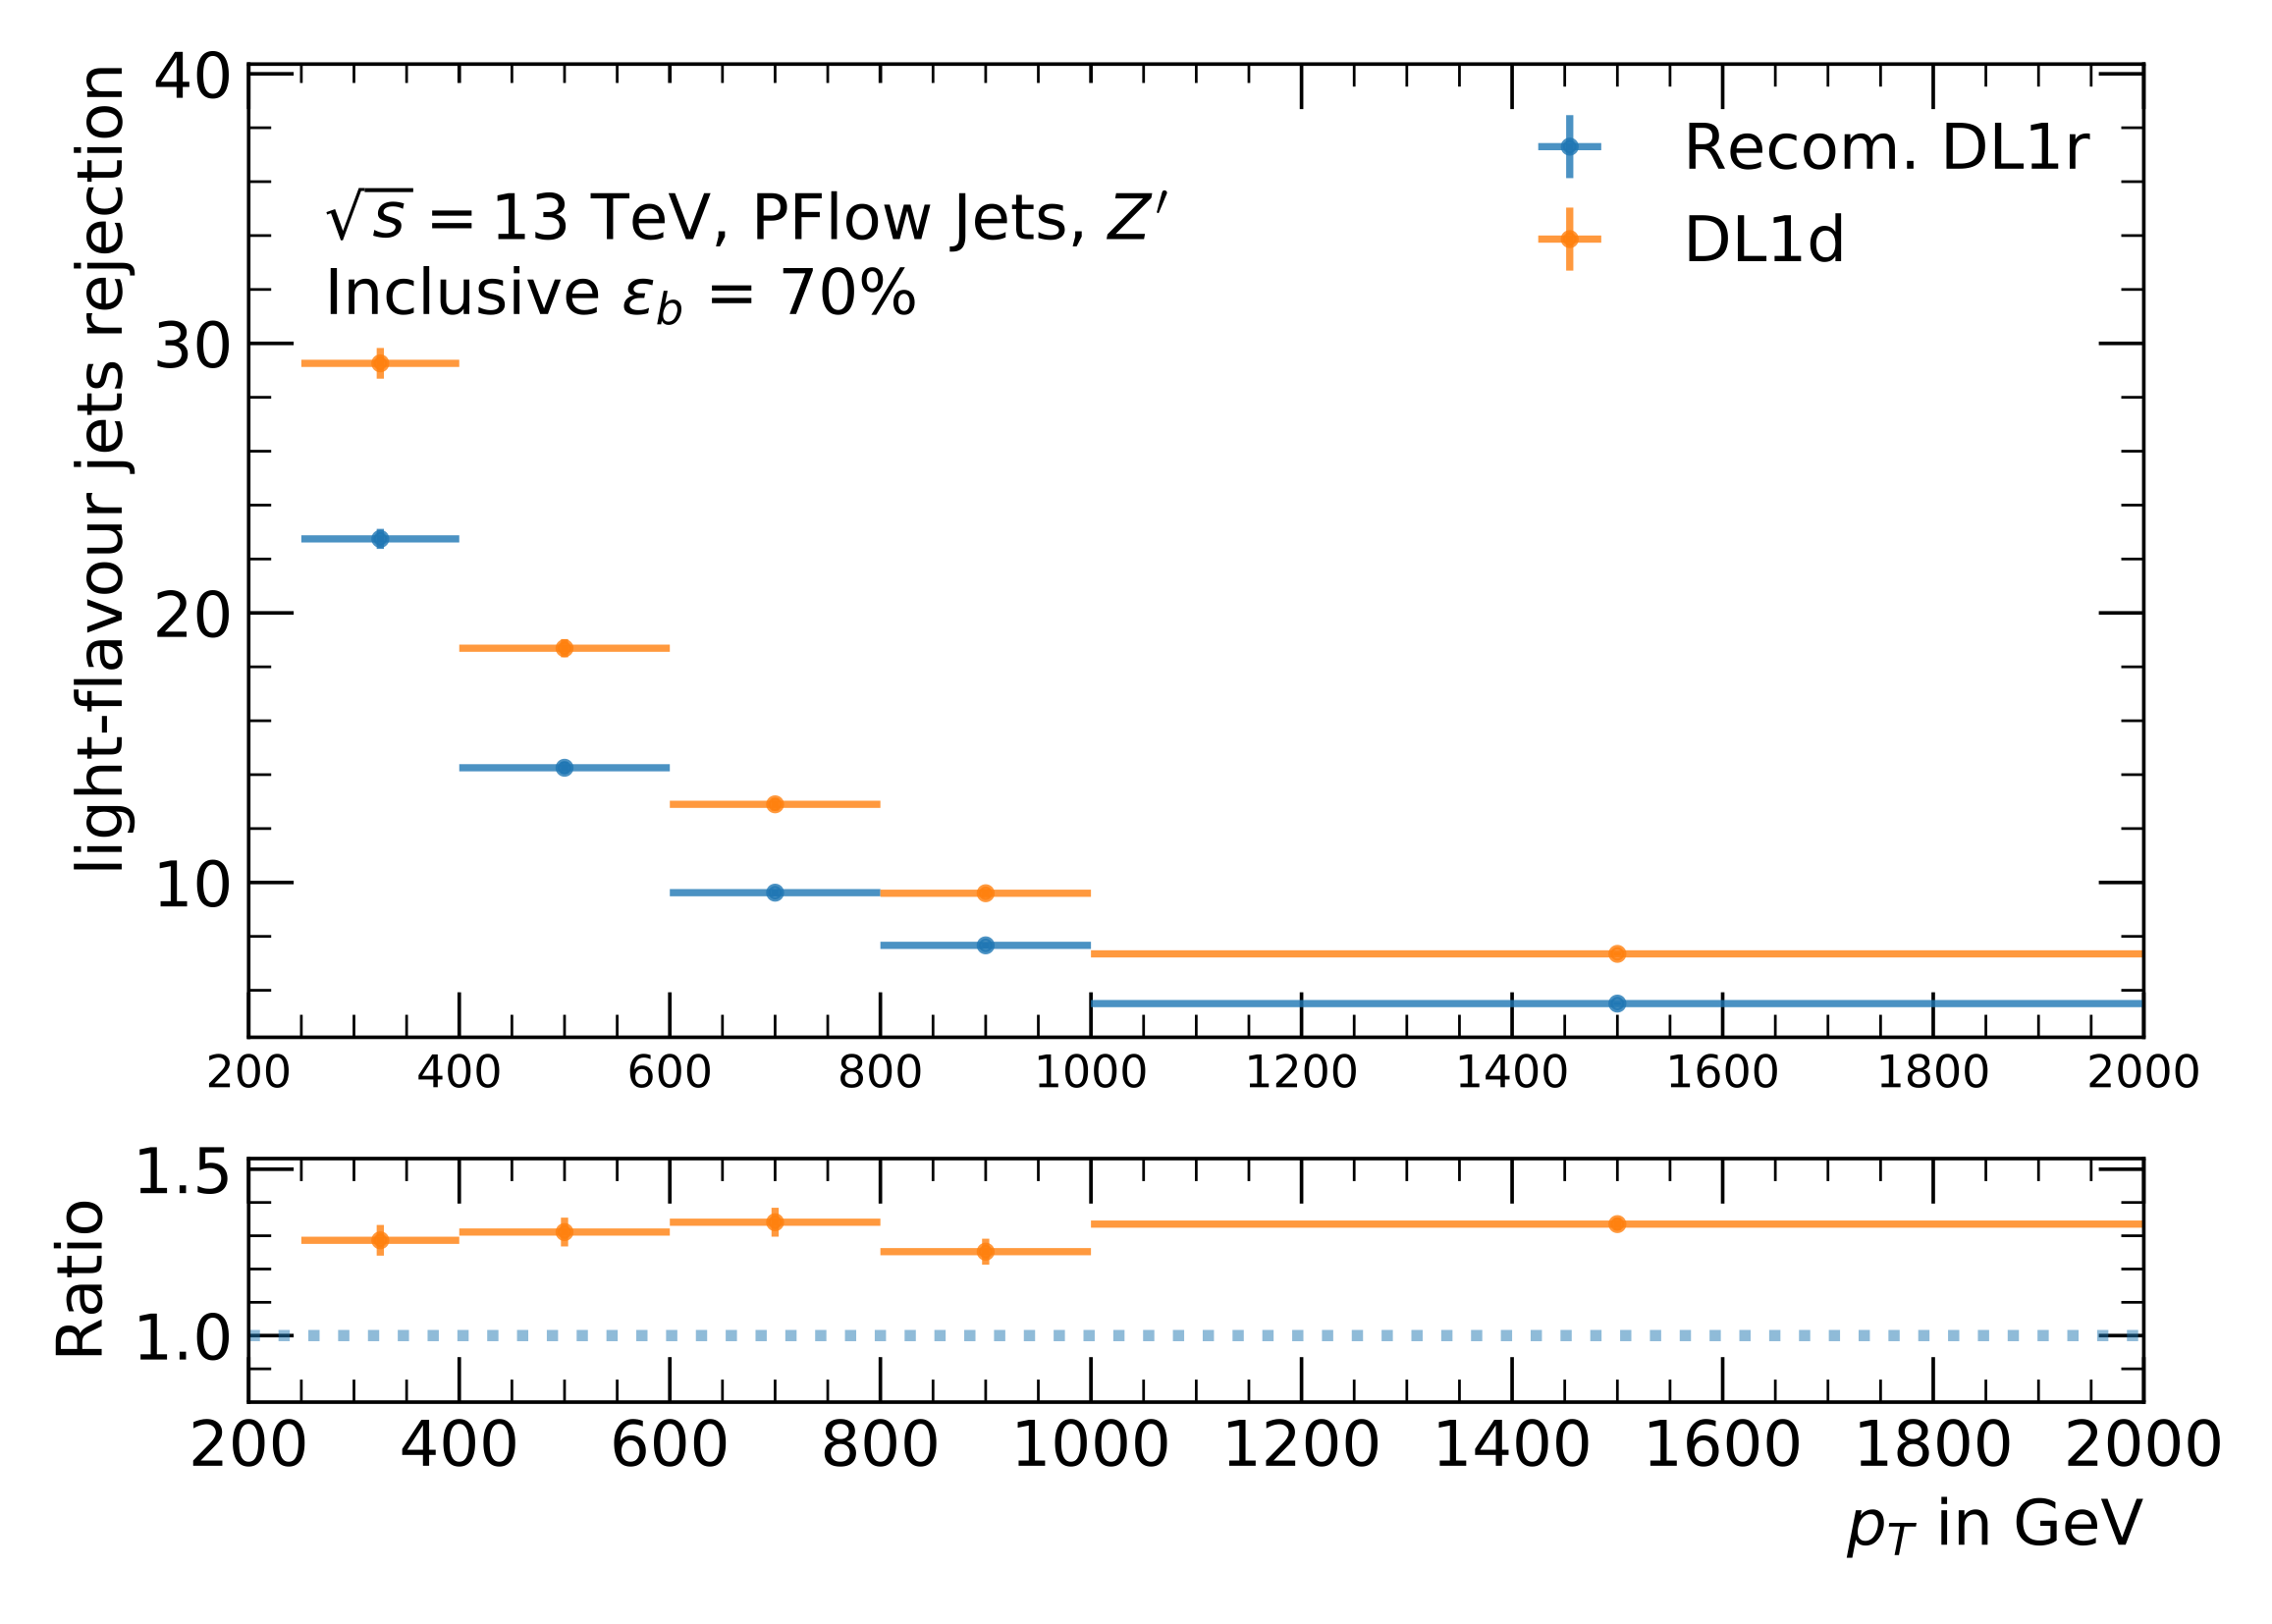
\includegraphics[scale=0.425]{Images/FTAG/DL1d/perpT/zpbu.png}
}
\caption{Background flavour rejections at a fixed $b$-tagging efficiency of 70\% (per region shown) for the various taggers. Top: $t\bar{t}$; bottom: $Z'$; left: $c$-rejection; right: light-rejection. For each plot, the bottom panel presents the ratio to the recommended \gls{dl1r}.}
\label{fig:ptDL1dtt}
\bigskip
\centerline{
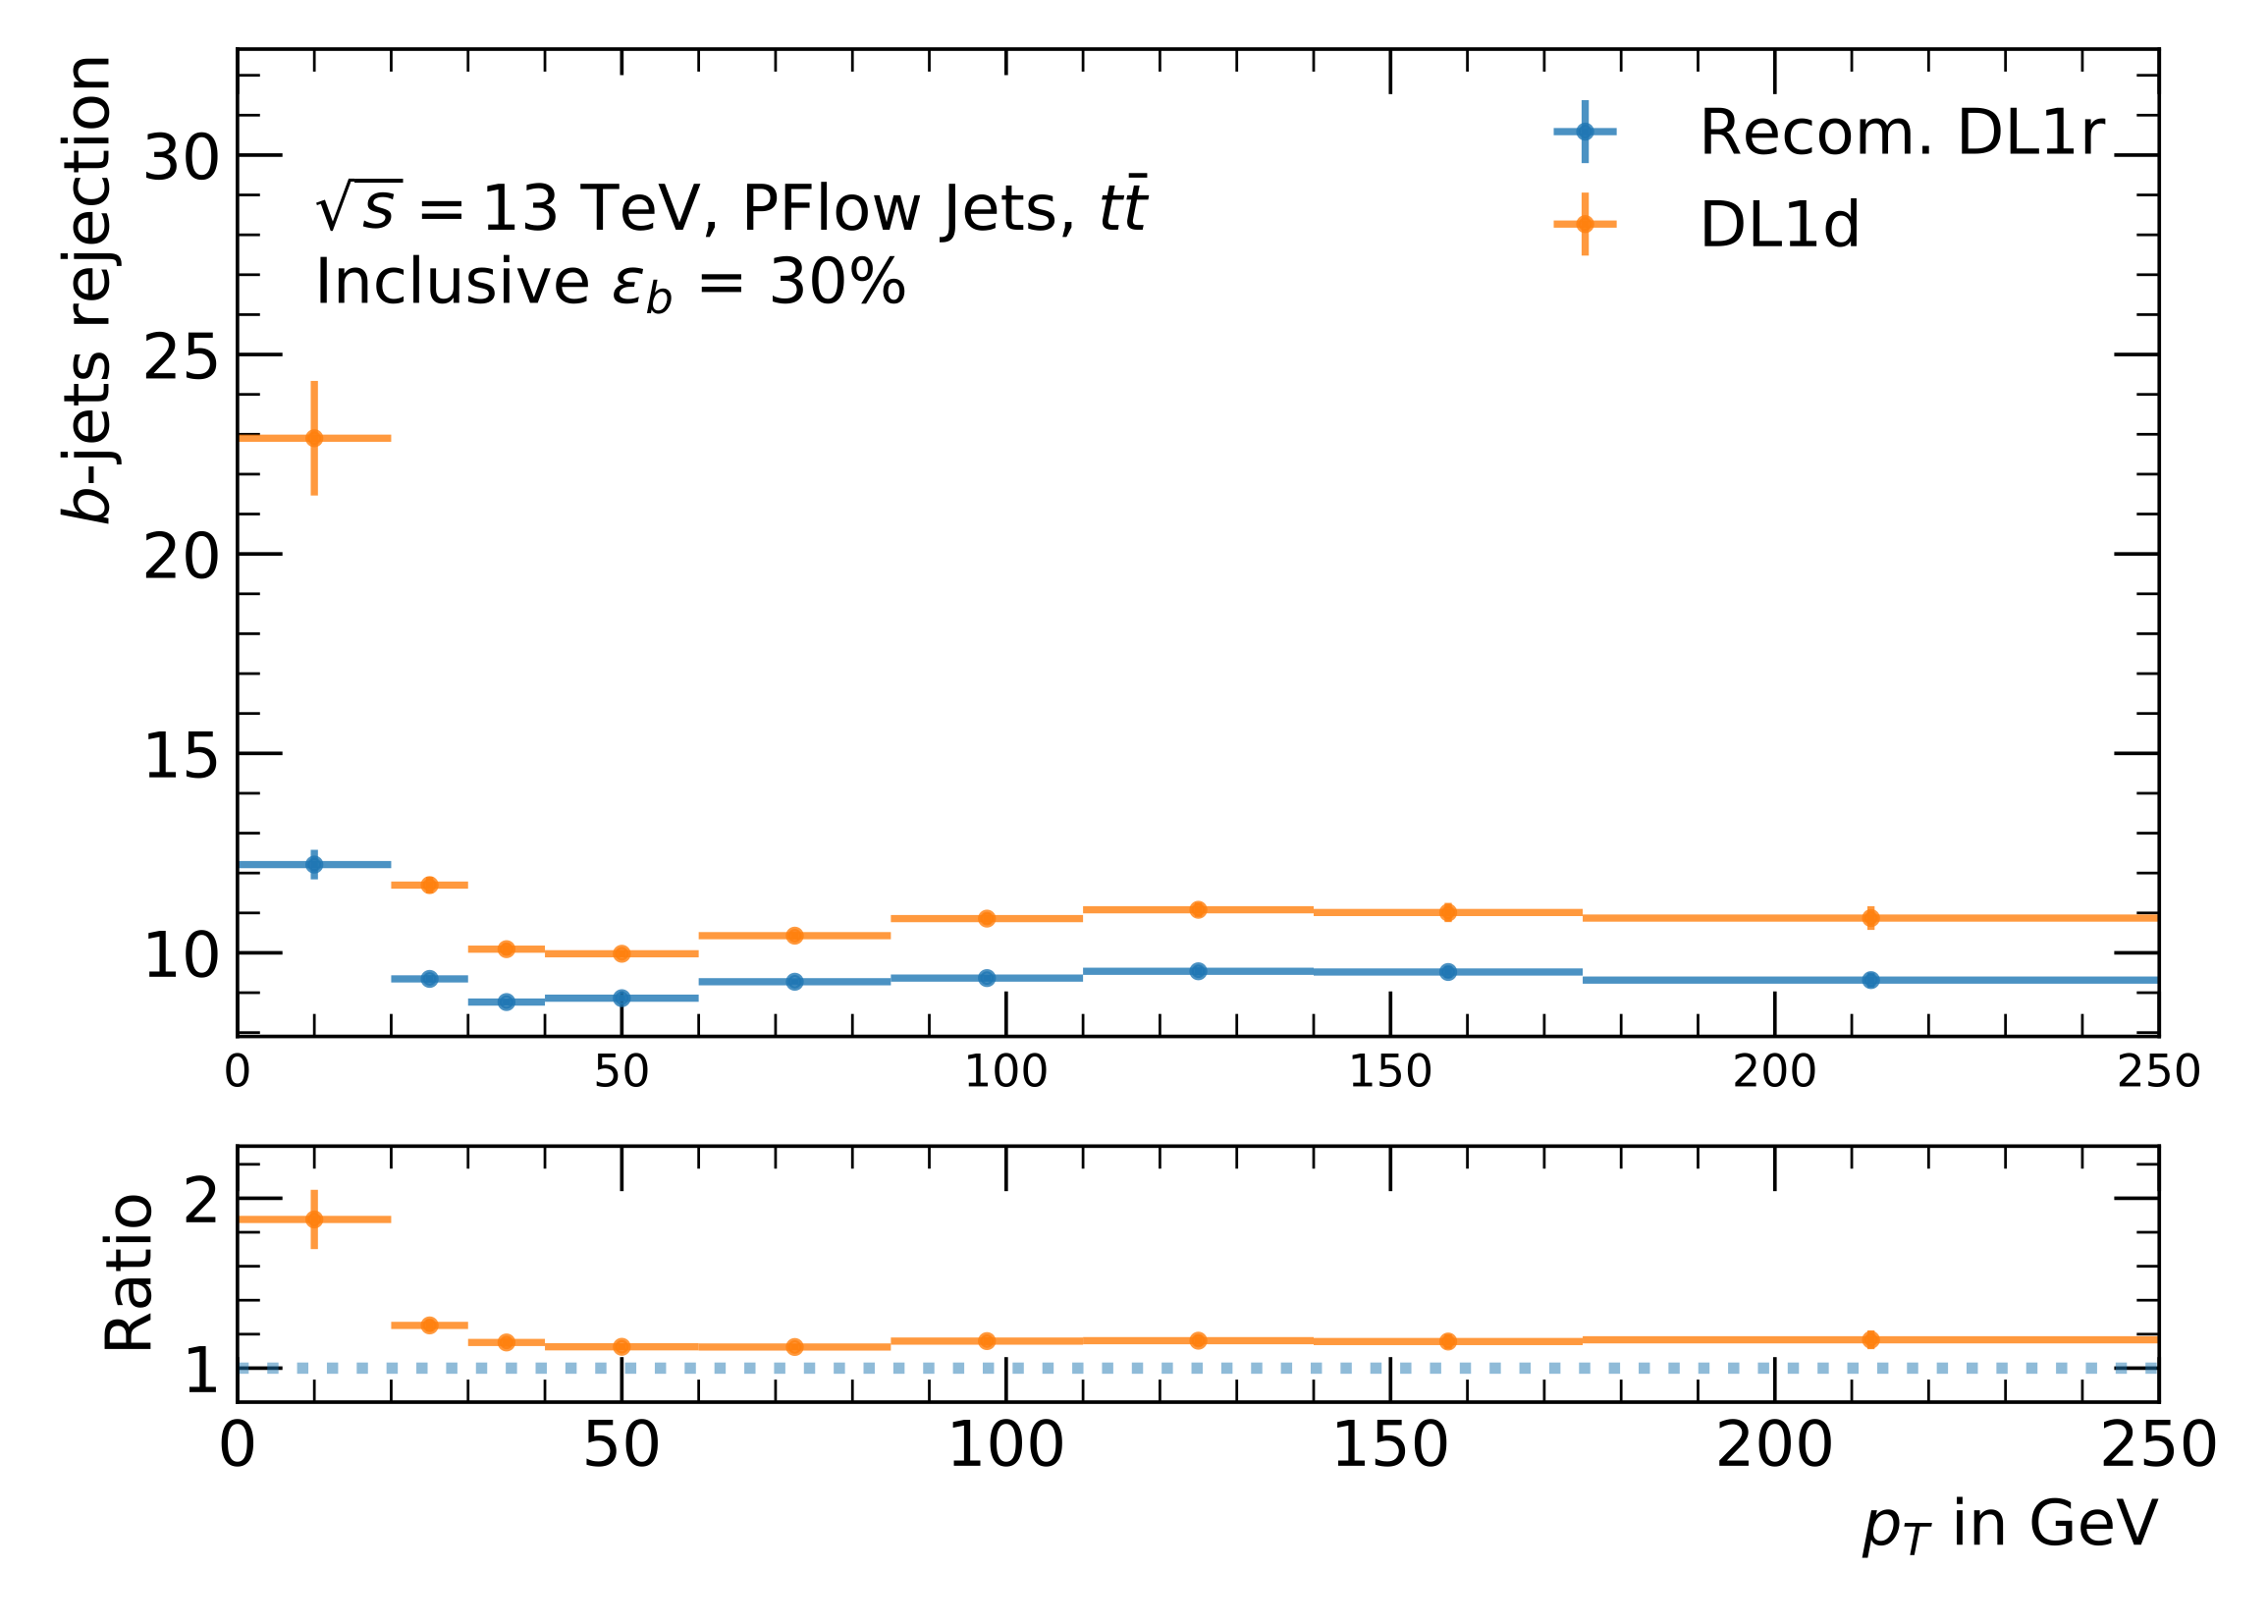
\includegraphics[scale=0.425]{Images/FTAG/DL1d/perpT/ttcb.png}
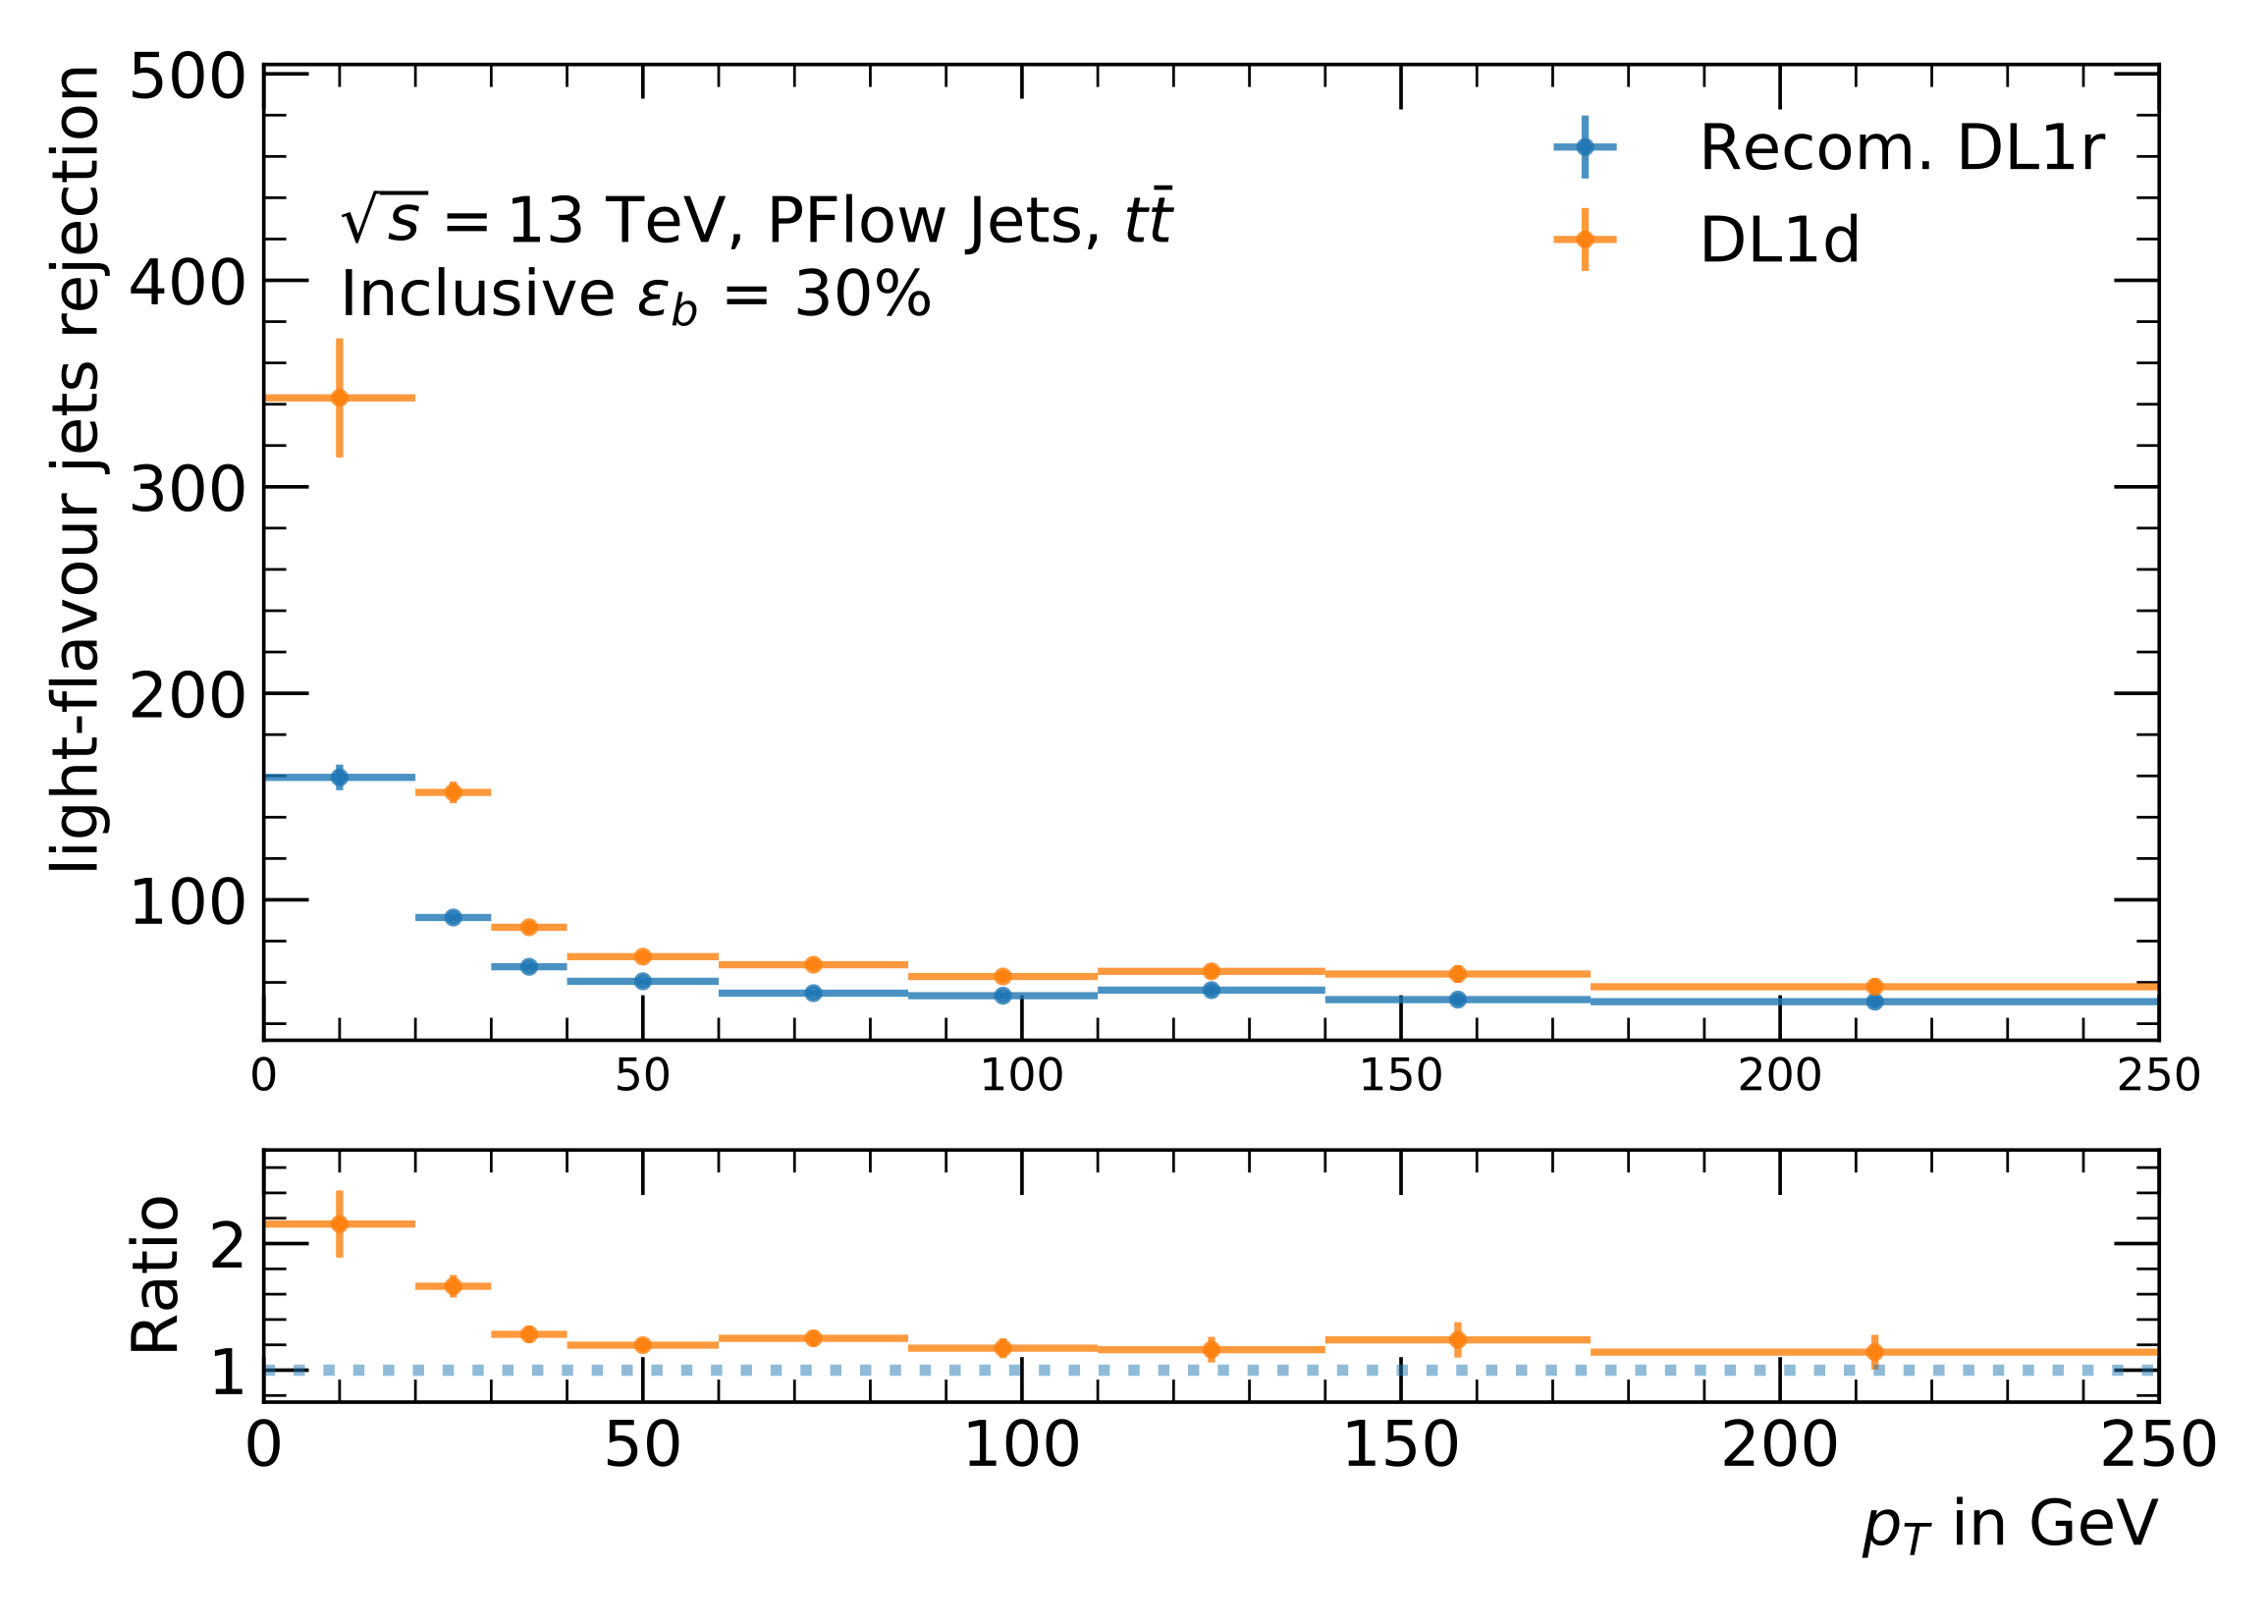
\includegraphics[scale=0.425]{Images/FTAG/DL1d/perpT/ttcu.png}}
\centerline{
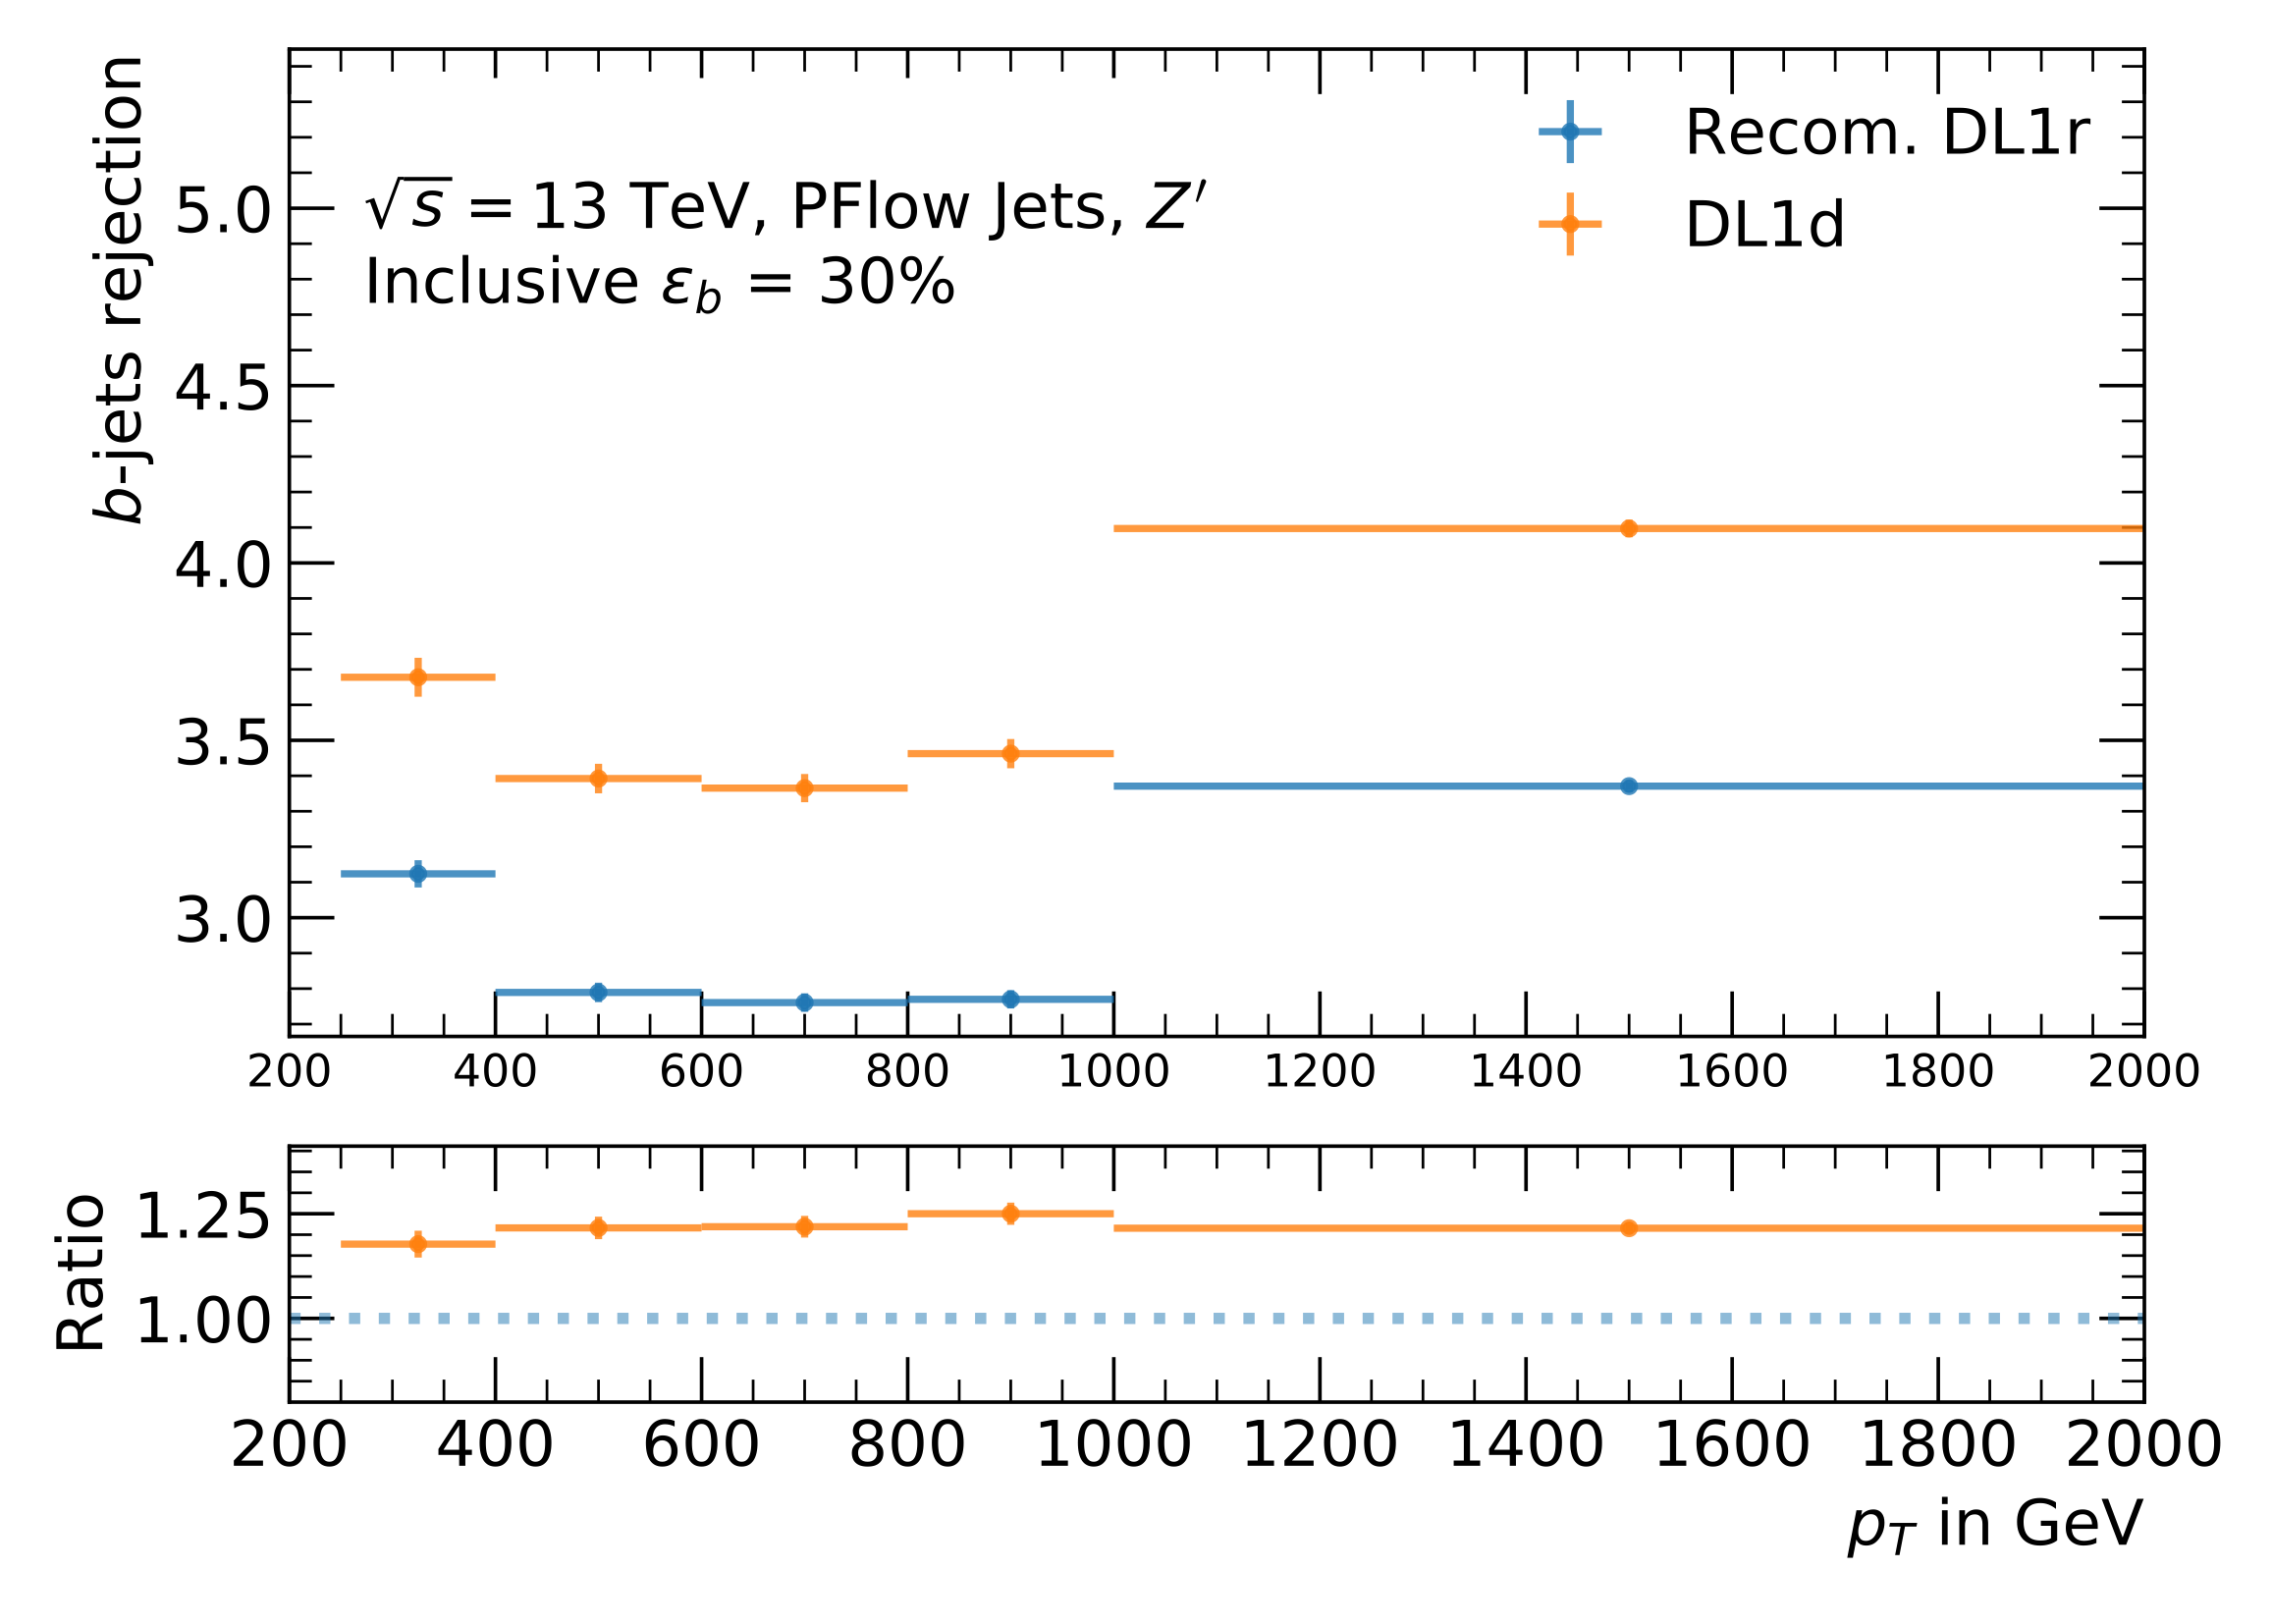
\includegraphics[scale=0.425]{Images/FTAG/DL1d/perpT/zpcb.png}
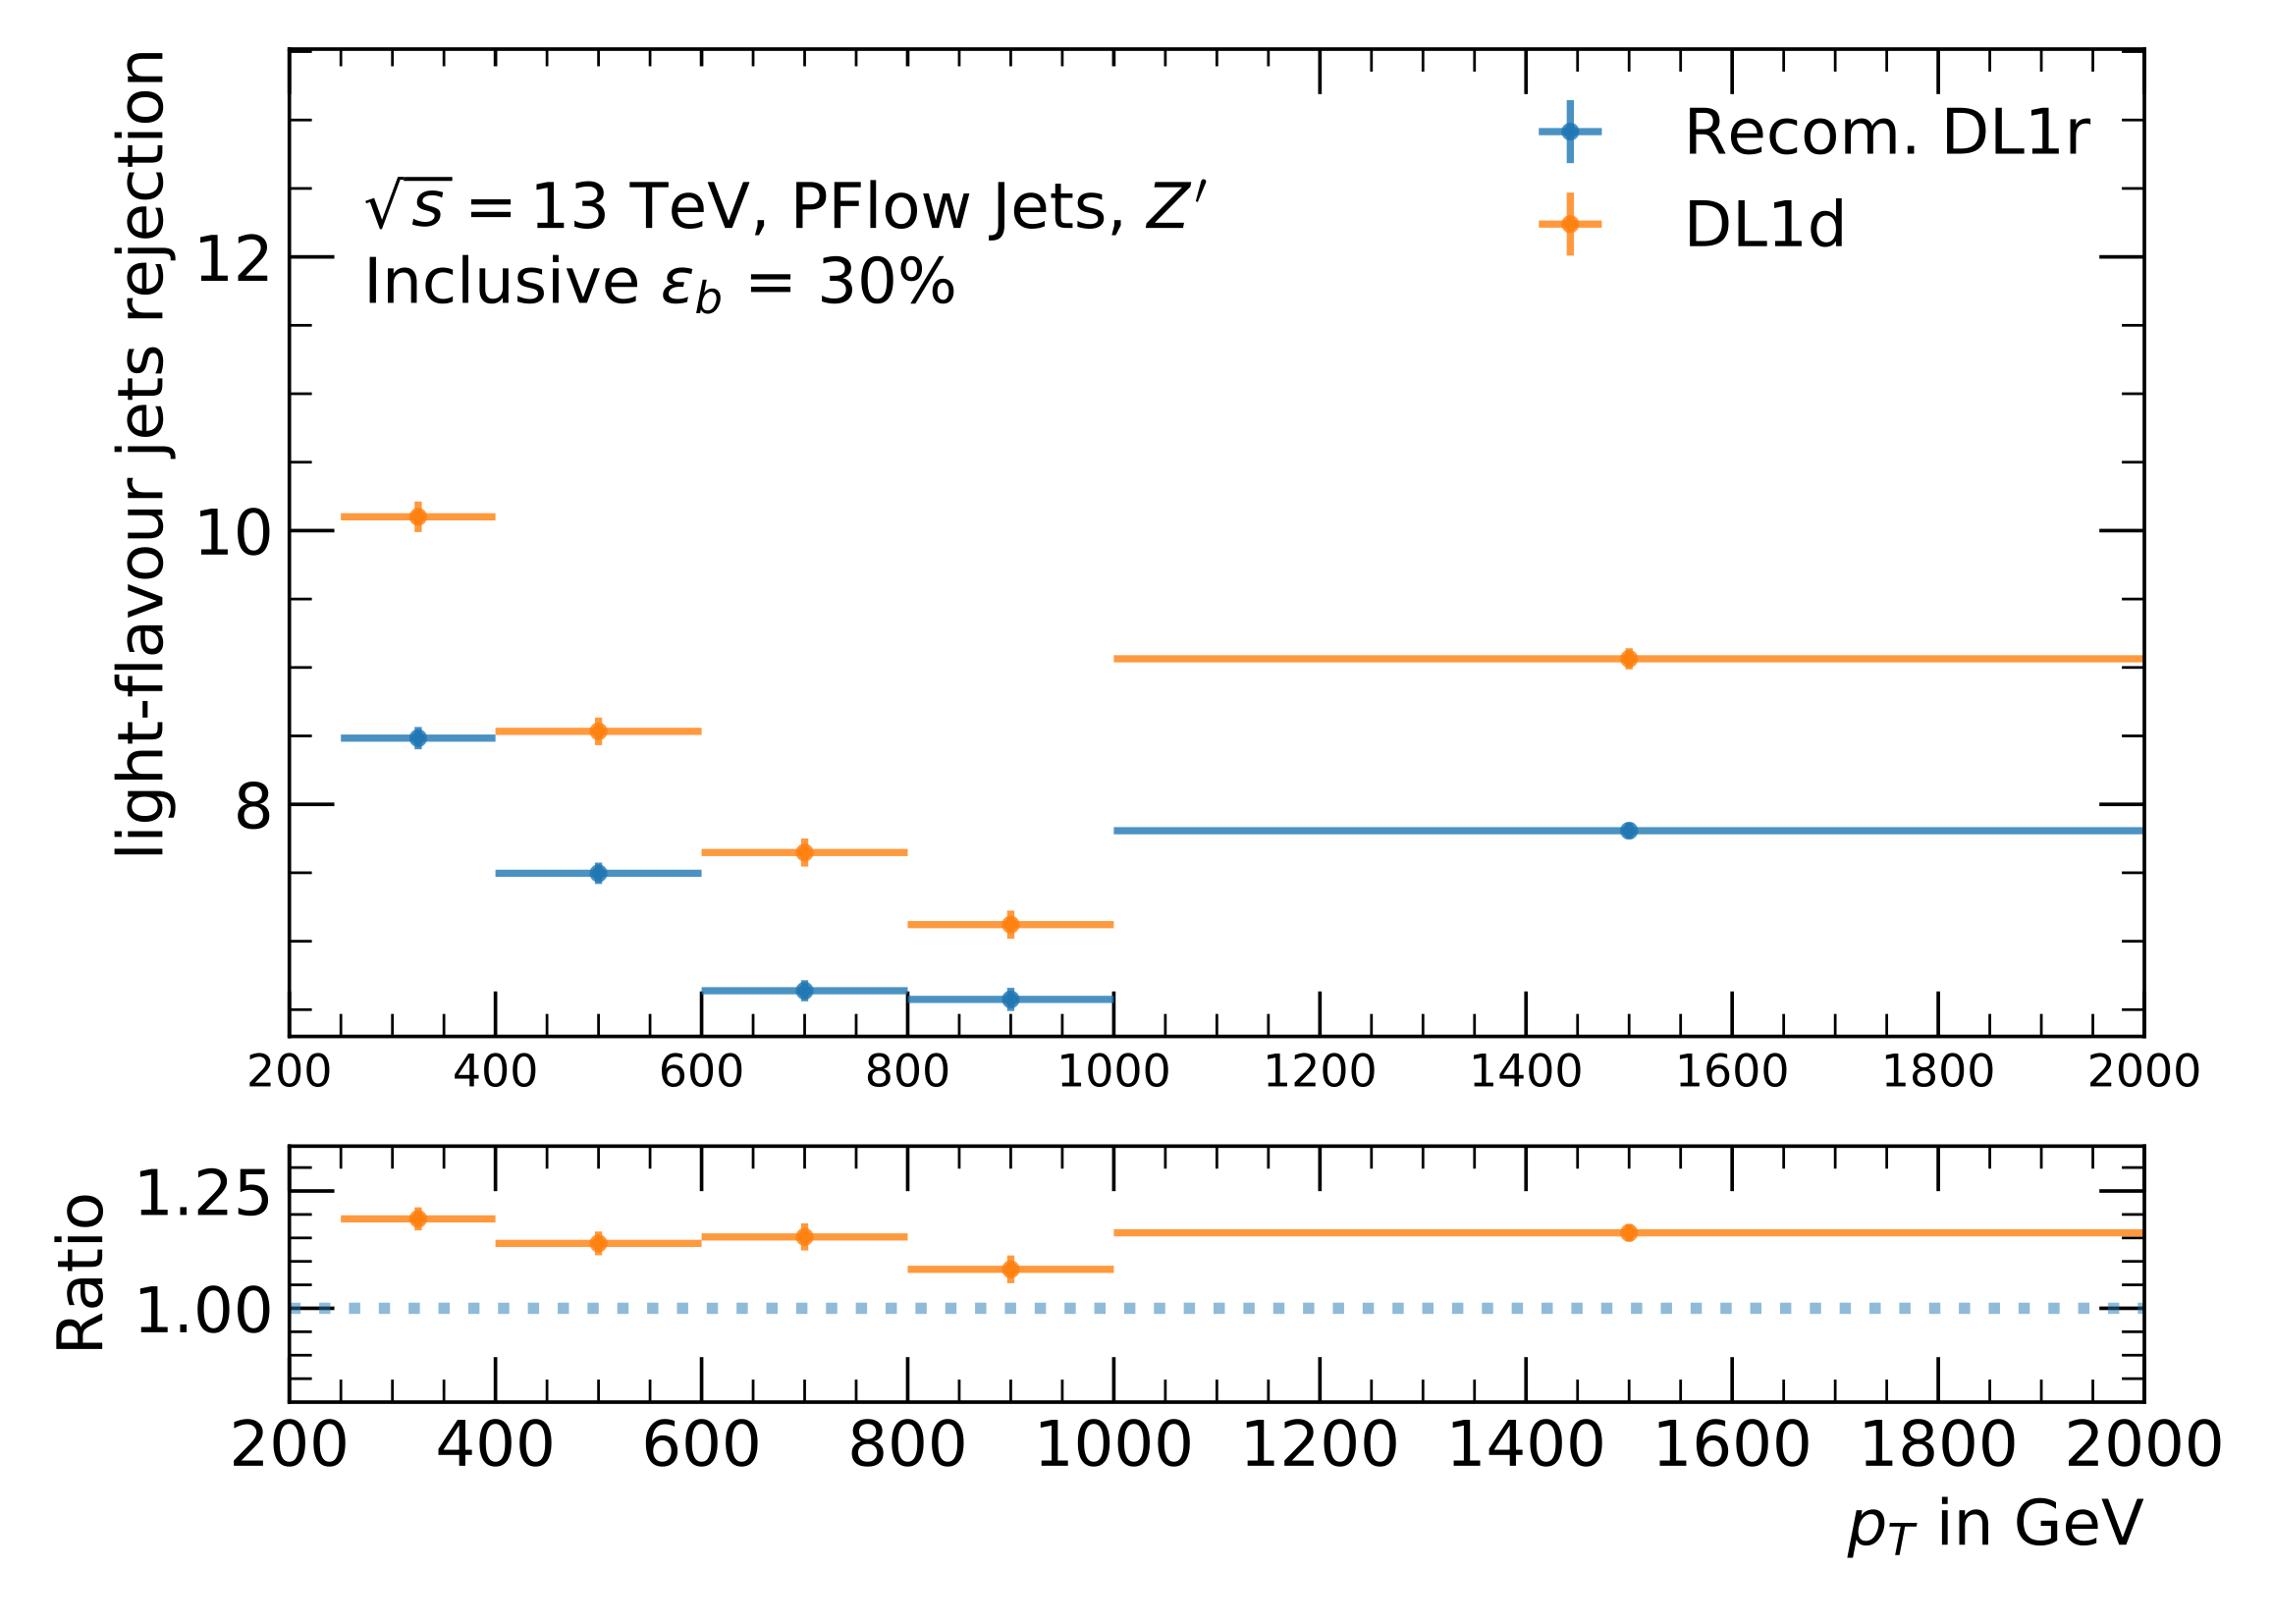
\includegraphics[scale=0.425]{Images/FTAG/DL1d/perpT/zpcu.png}
}
\caption{Background flavour rejections at a fixed $c$-tagging efficiency of 30\% (per region shown) for the various taggers. Top: $t\bar{t}$; bottom: $Z'$; left: $b$-rejection; right: light-rejection. For each plot, the bottom panel presents the ratio to the recommended \gls{dl1r}.}
\label{fig:ptDL1dz}
\end{figure}
\end{center}

In Figures \ref{fig:DL1dtt} and \ref{fig:DL1dz}, a GN-like tagger trained on 20 million jets from the new family base on \gls{gnn} that was in development at the time is introduced: \gls{gn1} \cite{ATL-PHYS-PUB-2022-027}. This model is based on a graph attention network (\gls{gat}) directly processing low-level inputs, thereby diverging from the traditional ATLAS flavour tagging philosophy of combining several low-level sub-taggers into a high-level one, such as in \gls{dl1d}. As examplified in this plot, the method offersa significant boost in performance and is explored in further details in Chapter \ref{chap:GN}. \\

The \gls{dl1d} model, integrating the Deep Set-based \gls{dips} network in the classical \gls{dl1} hierarchical approach, was a valuable step in the development of a modern performant flavour tagger for ATLAS. Thanks to its simularities with the previous \gls{dl1r} generation of tagger, built with the \gls{rnn}-based \gls{rnnip}, it was smoothly integrated in the processing pipeline of the flavour tagger group. Its quick callibration lead to its rapid introduction to the Collaboration that used it in several analyses, such as di-Higgs searches decaying to $b\bar{b}$ pairs and Run 3 analyses. To exploit the full potential of the trained model and to catter to specific needs of each experience, several working points were defined and calibrated. An important parameter to control the relative importance of the jet classes to be rejected with the discriminants of Equations \ref{bdisc} and \ref{cdisc}, light and $c$ for $b$-tagging and light and $b$ for $c$-tagging, are the flavour fractions $f_c$ and $f_b$. Naturally, this is a trade-of: for $b$-tagging, a larger $f_c$-value favorised a better $c$-rejection at the cost of a degraded light-rejection. To measure this dependency, flavour fractions scans are performed at a fixed $b$-tagging ($c$-tagging) efficiency of 77\% (30\%) in Figure \ref{fig:DL1dscanfb} (Figure \ref{fig:DL1dscanfc}). % NEED ref of the di-higgs used of DL1d

\begin{figure}[h!]
  \centering
  \begin{subfigure}[b]{\textwidth}
      \centering
      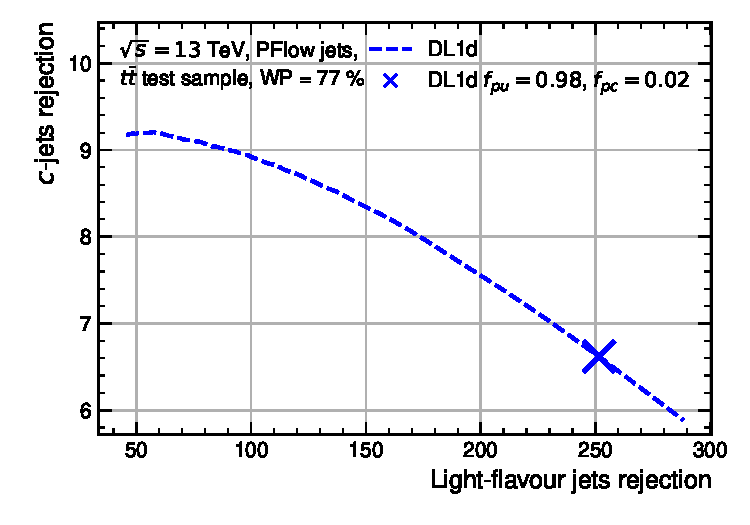
\includegraphics[width=0.49\textwidth]{Images/FTAG/DL1d/extra_plots/contour_fraction_ttbar_300.pdf}
      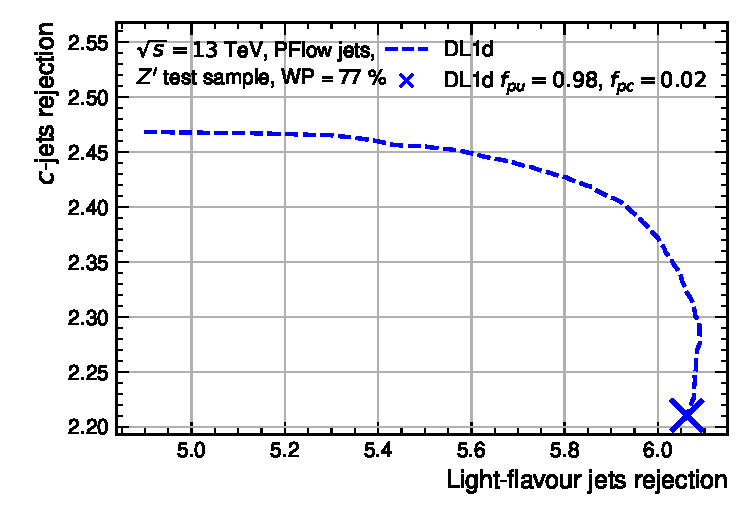
\includegraphics[width=0.49\textwidth]{Images/FTAG/DL1d/extra_plots/contour_fraction_zp_300.pdf}
      \caption{Flavour fraction $f_c^b$ for $b$-tagging scan: left is $t\bar{t}$ and right $Z'$ test samples.} 
      \label{fig:DL1dscanfb}
  \end{subfigure}\\
  \begin{subfigure}[b]{\textwidth}
    \centering % NEED TO CORRECT THE WP for the c-tagging case
    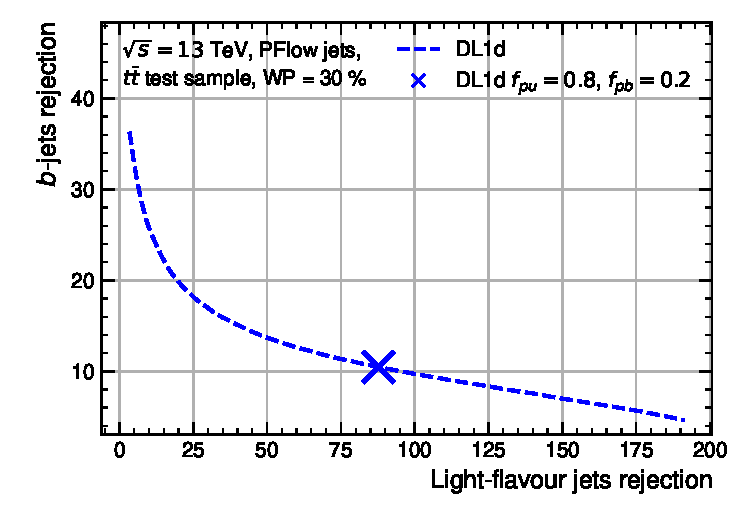
\includegraphics[width=0.49\textwidth]{Images/FTAG/DL1d/extra_plots/contour_fraction_c_ttbar_299.pdf}
    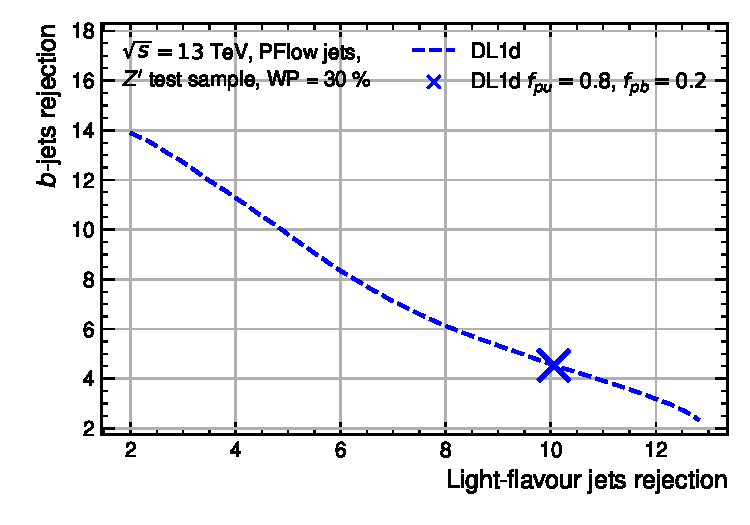
\includegraphics[width=0.49\textwidth]{Images/FTAG/DL1d/extra_plots/contour_fraction_c_zp_299.pdf}
    \caption{Flavour fraction $f_b^c$ for $c$-tagging scan: left is $t\bar{t}$ and right $Z'$ test samples.} 
    \label{fig:DL1dscanfc}
\end{subfigure}
  \caption{The flavour fraction scans of the DL1d model. The chosen values are marked on the curves, displaying on the $y$-axis the $c$-rejection ($b$-rejection) for $b$-tagging ($c$-tagging) vs the light-rejection on the $x$ axis at a fixed working point of 77\% (33\%). Increasing $f_c$ or $f_b$ shifts the marker upwards along the curves. }
  \label{fig:DL1dscanf}
\end{figure} 

With regard to interpretability, it is of course challeging to outright explain the decision process underscoring the predictions of \gls{dl1d}. An effective technique to measure the relative importance of the different variables is to quantify their contribution to the output using Shapley values \cite{Rozemberczki2022TheSV}. This technique for model explanation calculates the average contribution of each input to the output \cite{Rozemberczki2022TheSV}. Figures \ref{fig:DL1dshapb} and \ref{fig:DL1dshapc} present the outcome of applying the framework proposed in Ref. \cite{NIPS2017_7062} to approximate the Shapley values of the inputs to the $b$-tagging $D_b$ and $c$-tagging $D_c$ discriminants of \gls{dl1d}. These so-called \textit{beeswarm} plots measure the impact of the evidence on the output of the model for each input feature. The plots display how each feature' Shapley value modifies the discriminant by moving from a prior background-data distribution expectation to the final model prediction using the real feature. A set of test datapoints of the targeted jet distributions are sampled and, for each, a prior expectation was randomly sampled for the initial test and the impact of using the real value was measured. Positive Shapley values indicate variables having an increasing effect on the discriminant, thereby helping either $b$- or $c$ tagging as per the plot considered. Each datapoint is coloured on a gradient scale from low- eature value in blue to high feature value in red, and the dots pile up to show density of the distribution. A feature that has a more weight of its Shapley values distribution at larger values of the feature can be expected to help the model in identifying the main flavour of jets. Conversely, if for large values of the feature the Shapley values are negative, the feature value should be lowered for the model discriminant to improve. 

%\begin{figure}[h!]
\begin{sidewaysfigure}
  \centering
  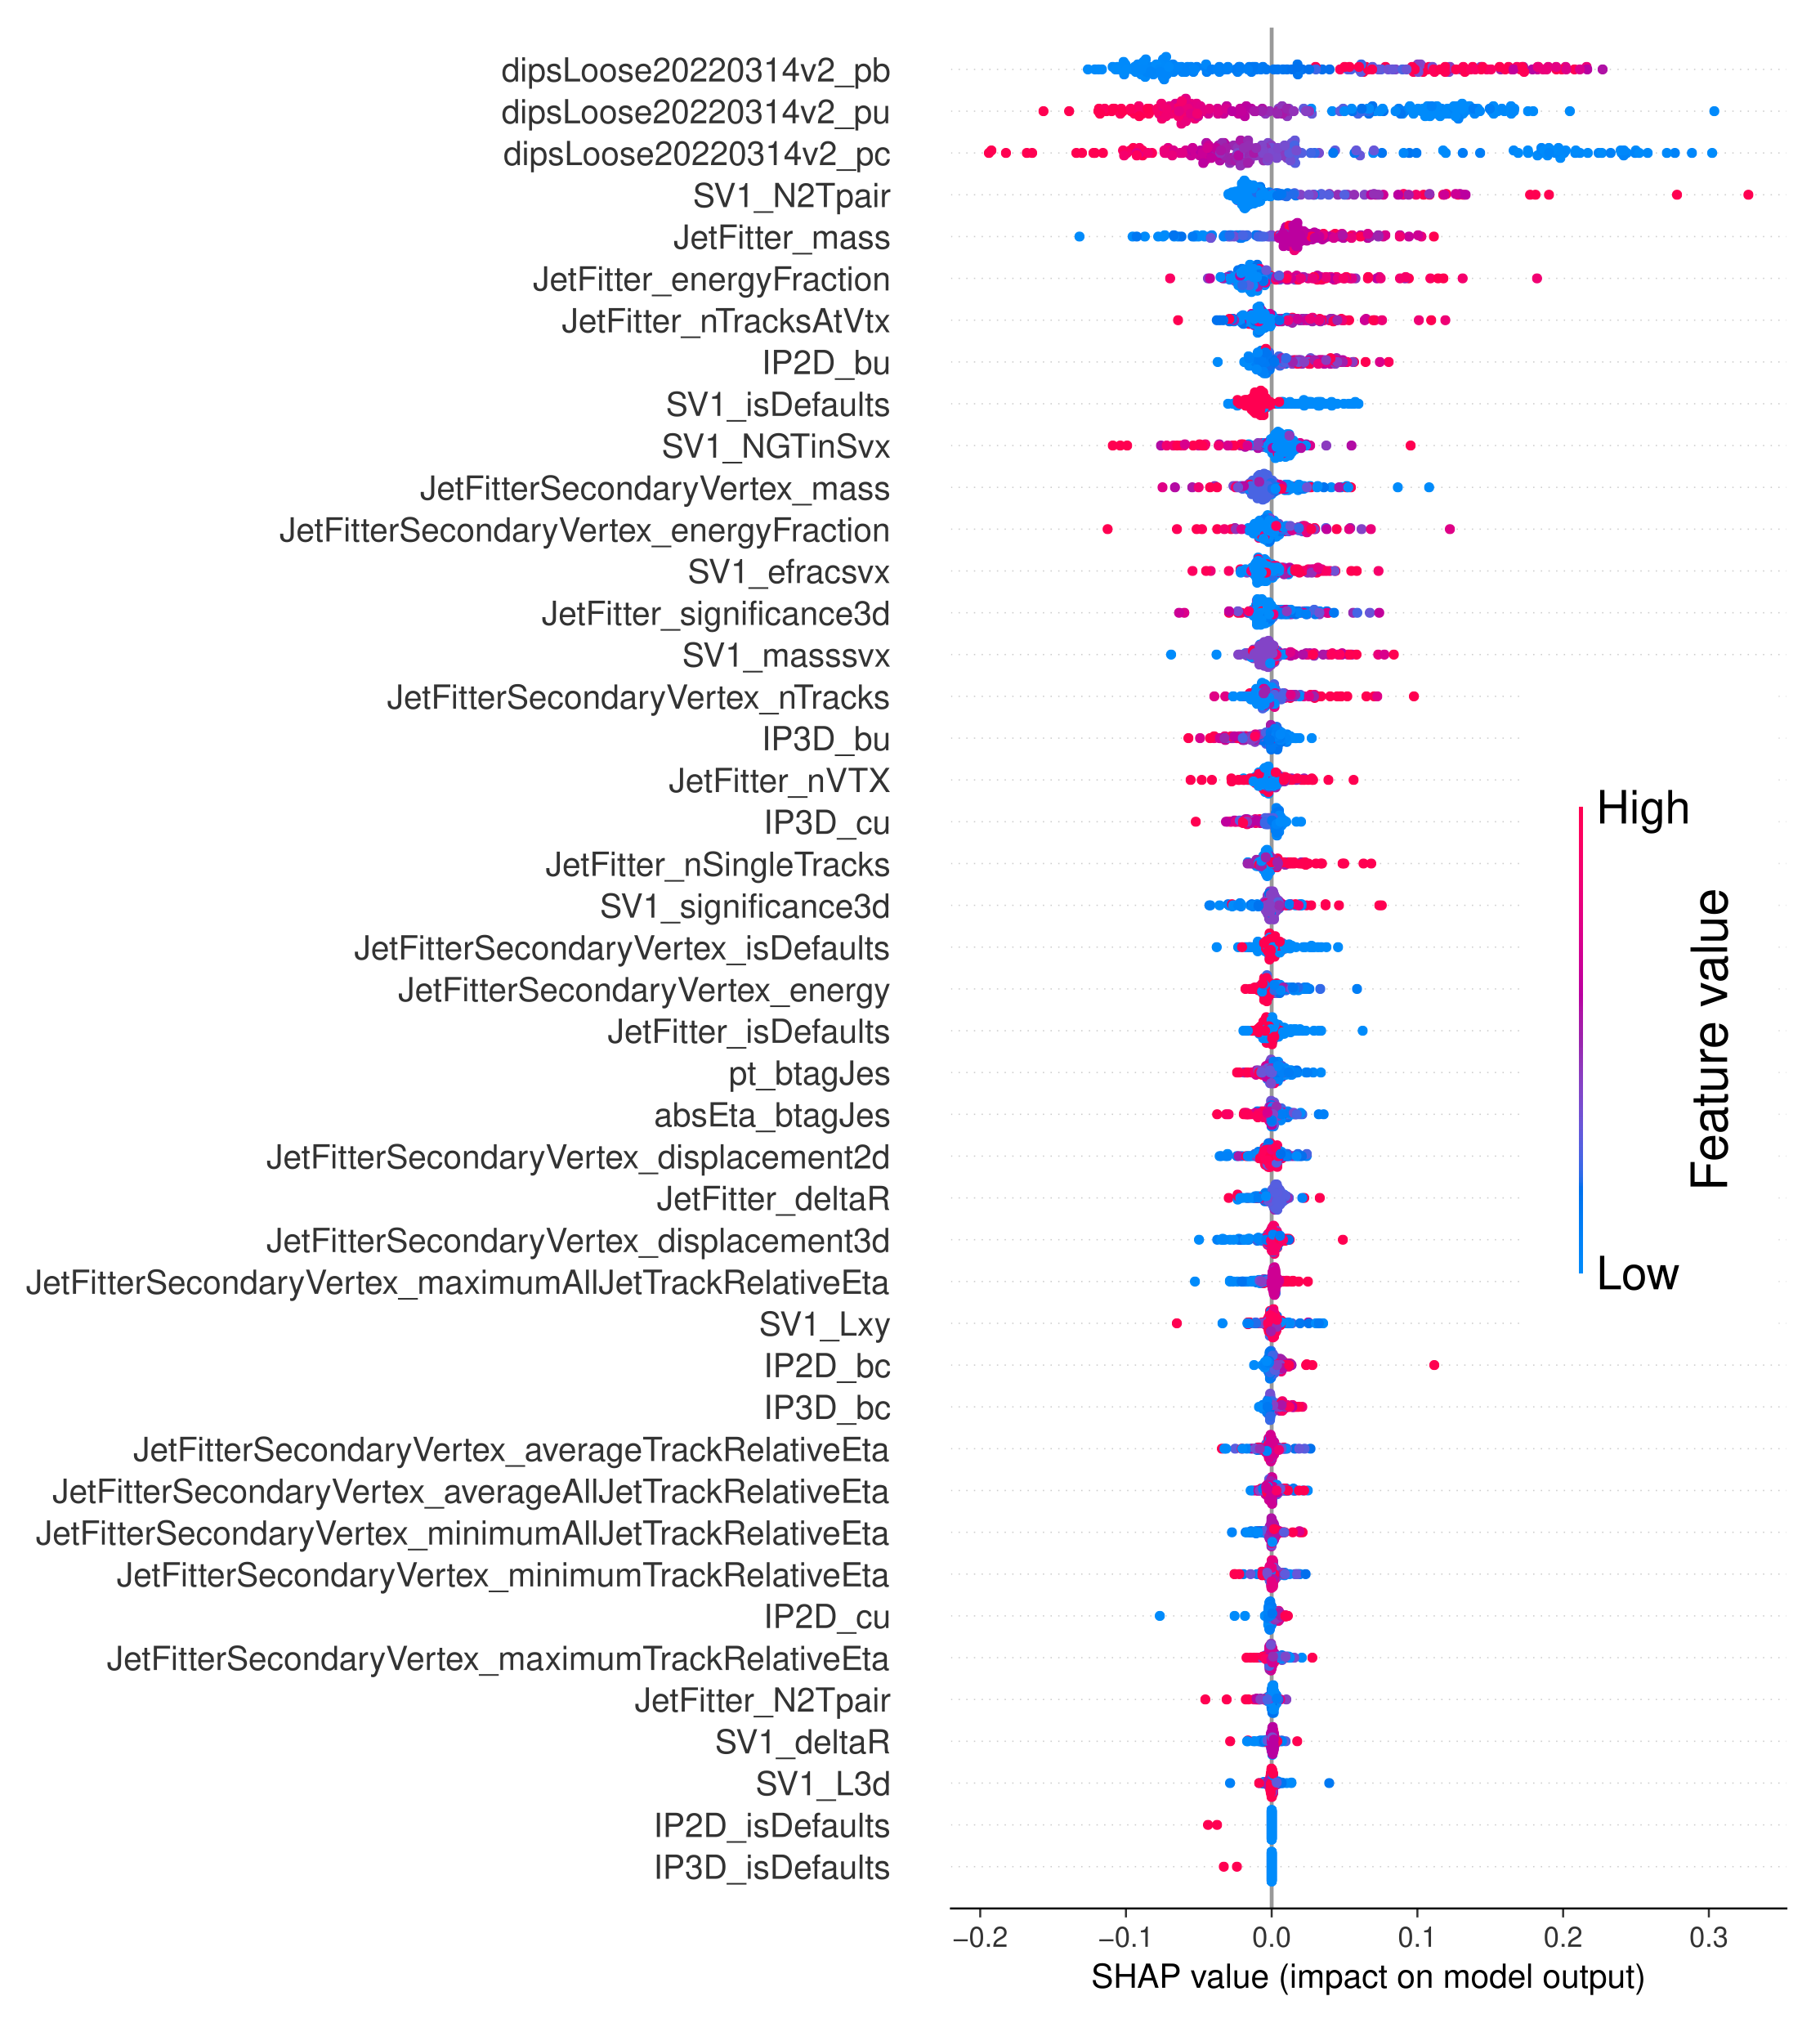
\includegraphics[scale=0.7]{Images/FTAG/DL1d/Shap/ttb.png}
  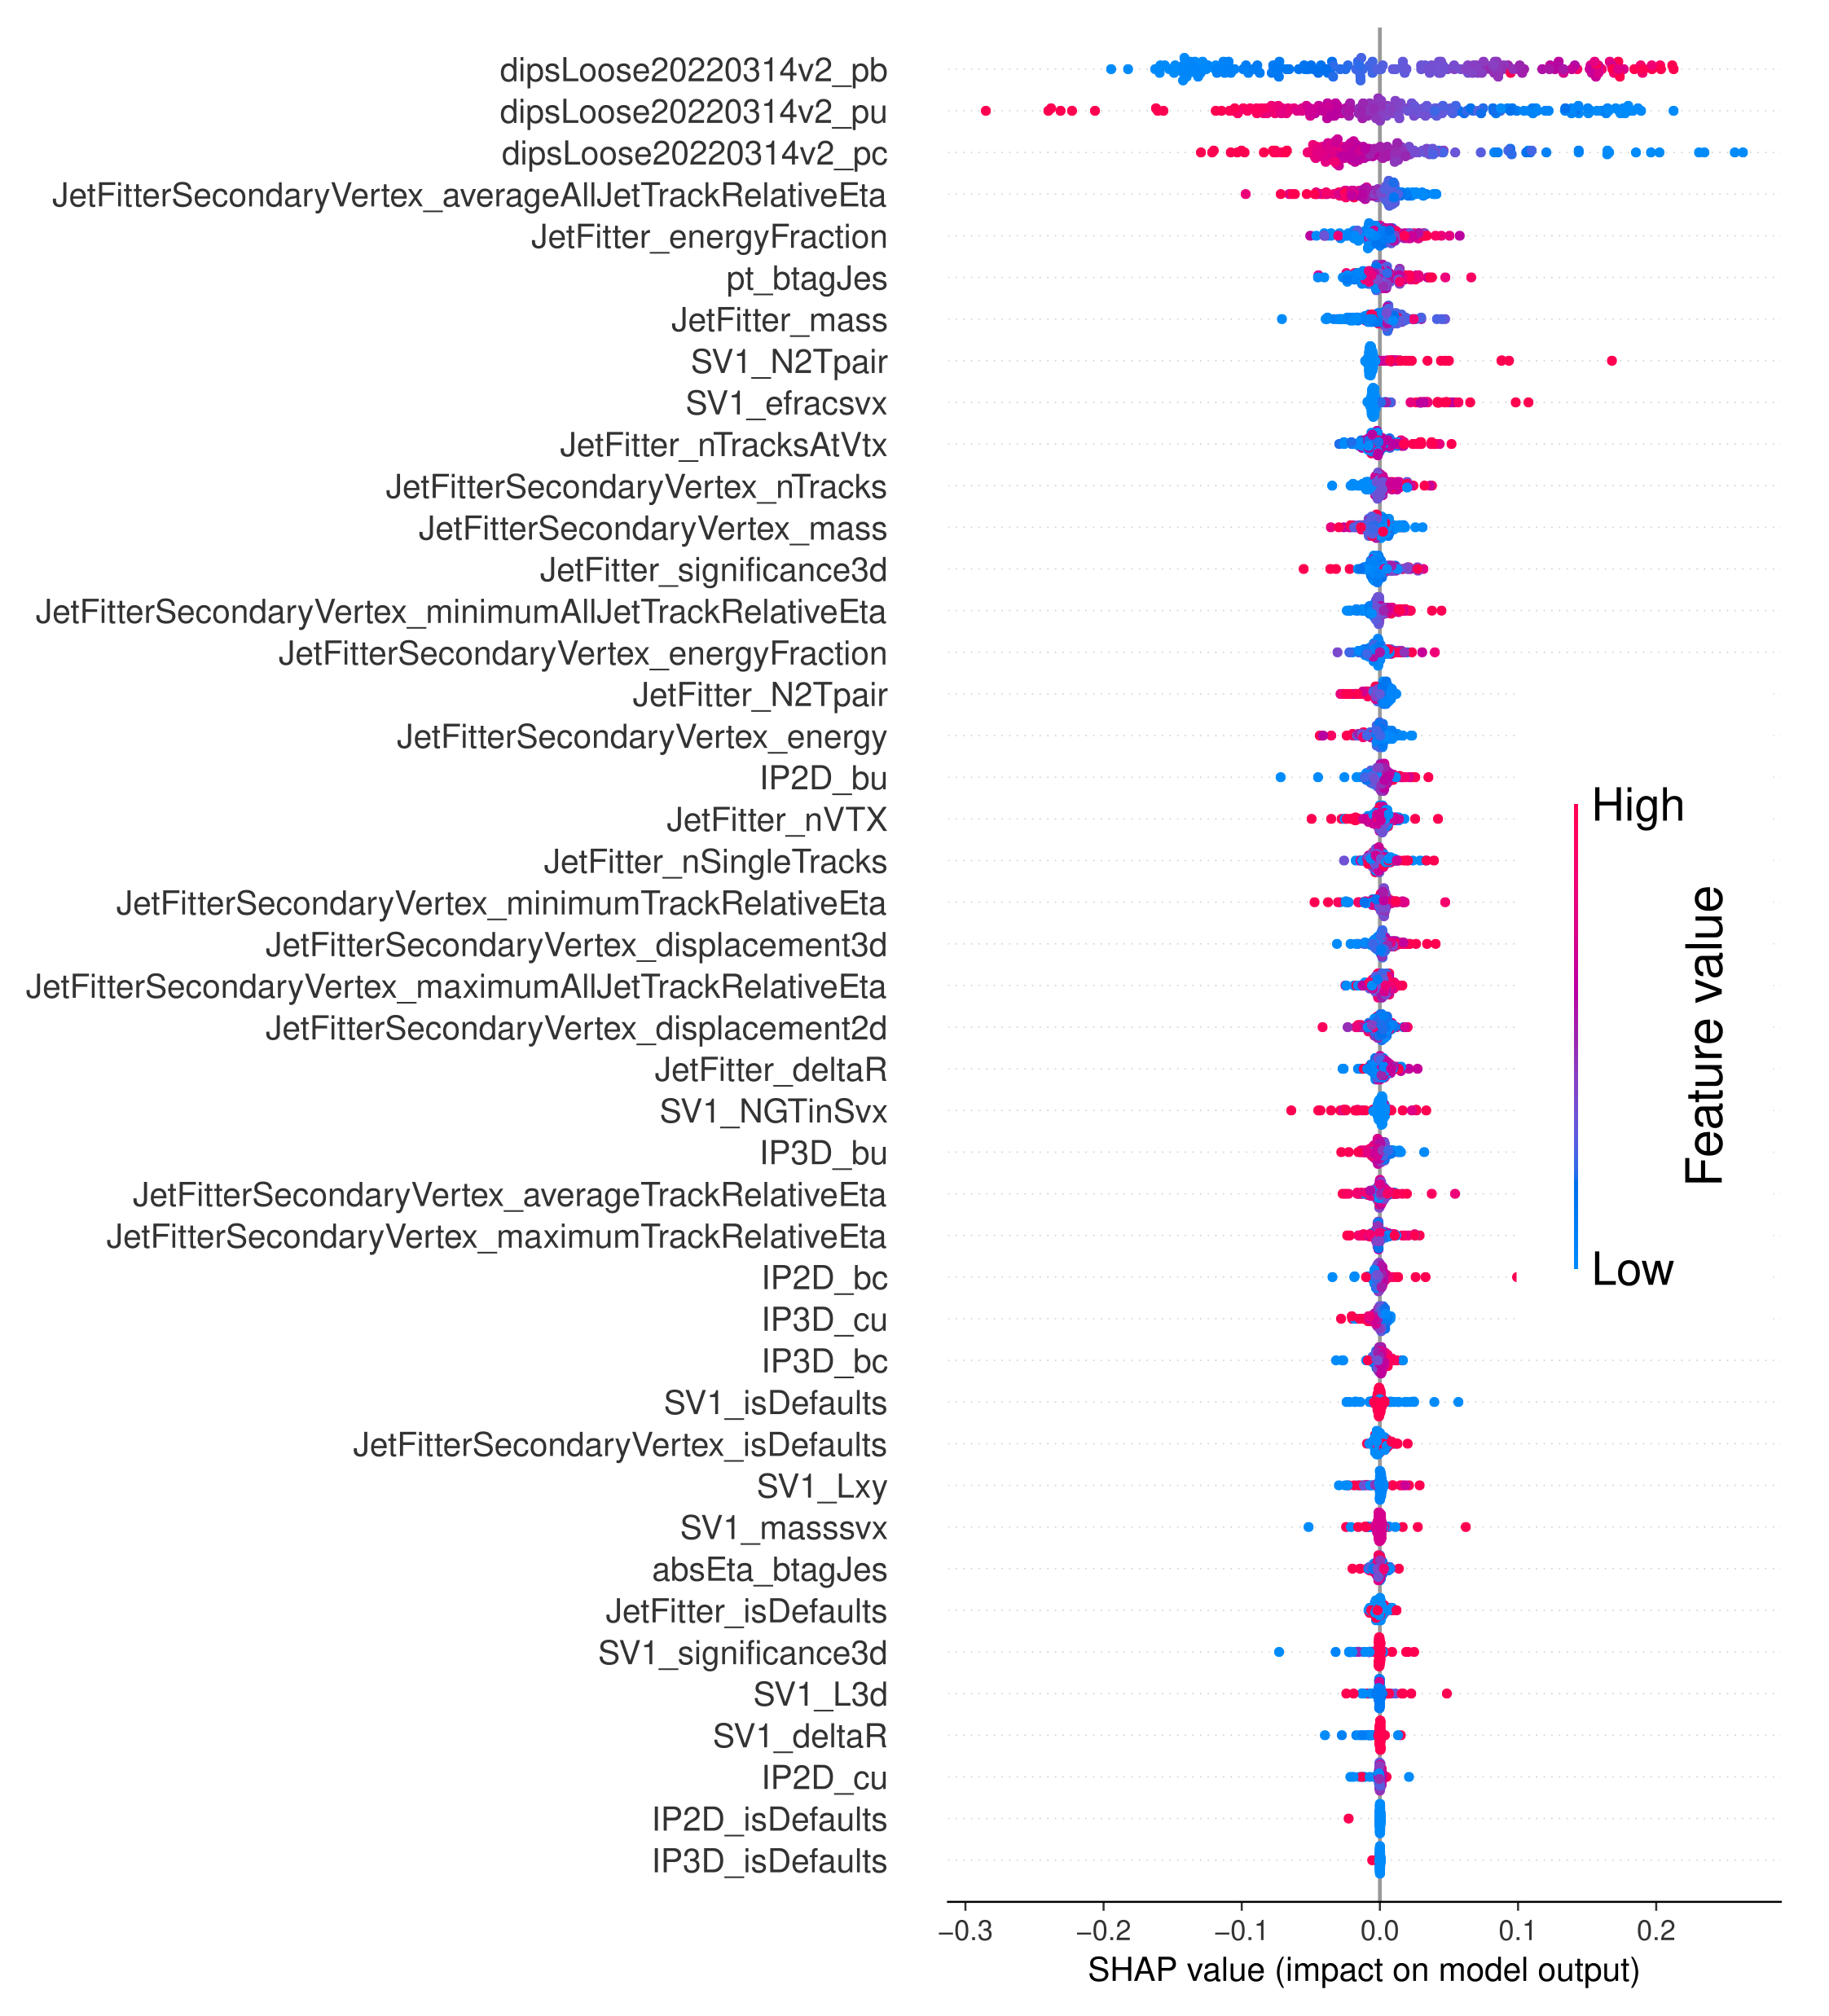
\includegraphics[scale=0.7]{Images/FTAG/DL1d/Shap/zpb.png}
  \caption{Shapley values of the different inputs variables of DL1d for $b$-tagging, $t\bar{t}$ on the left and $Z'$ on the right.} 
  \label{fig:DL1dshapb}
\end{sidewaysfigure} 


%\begin{figure}[h!]
\begin{sidewaysfigure}
  \centering
  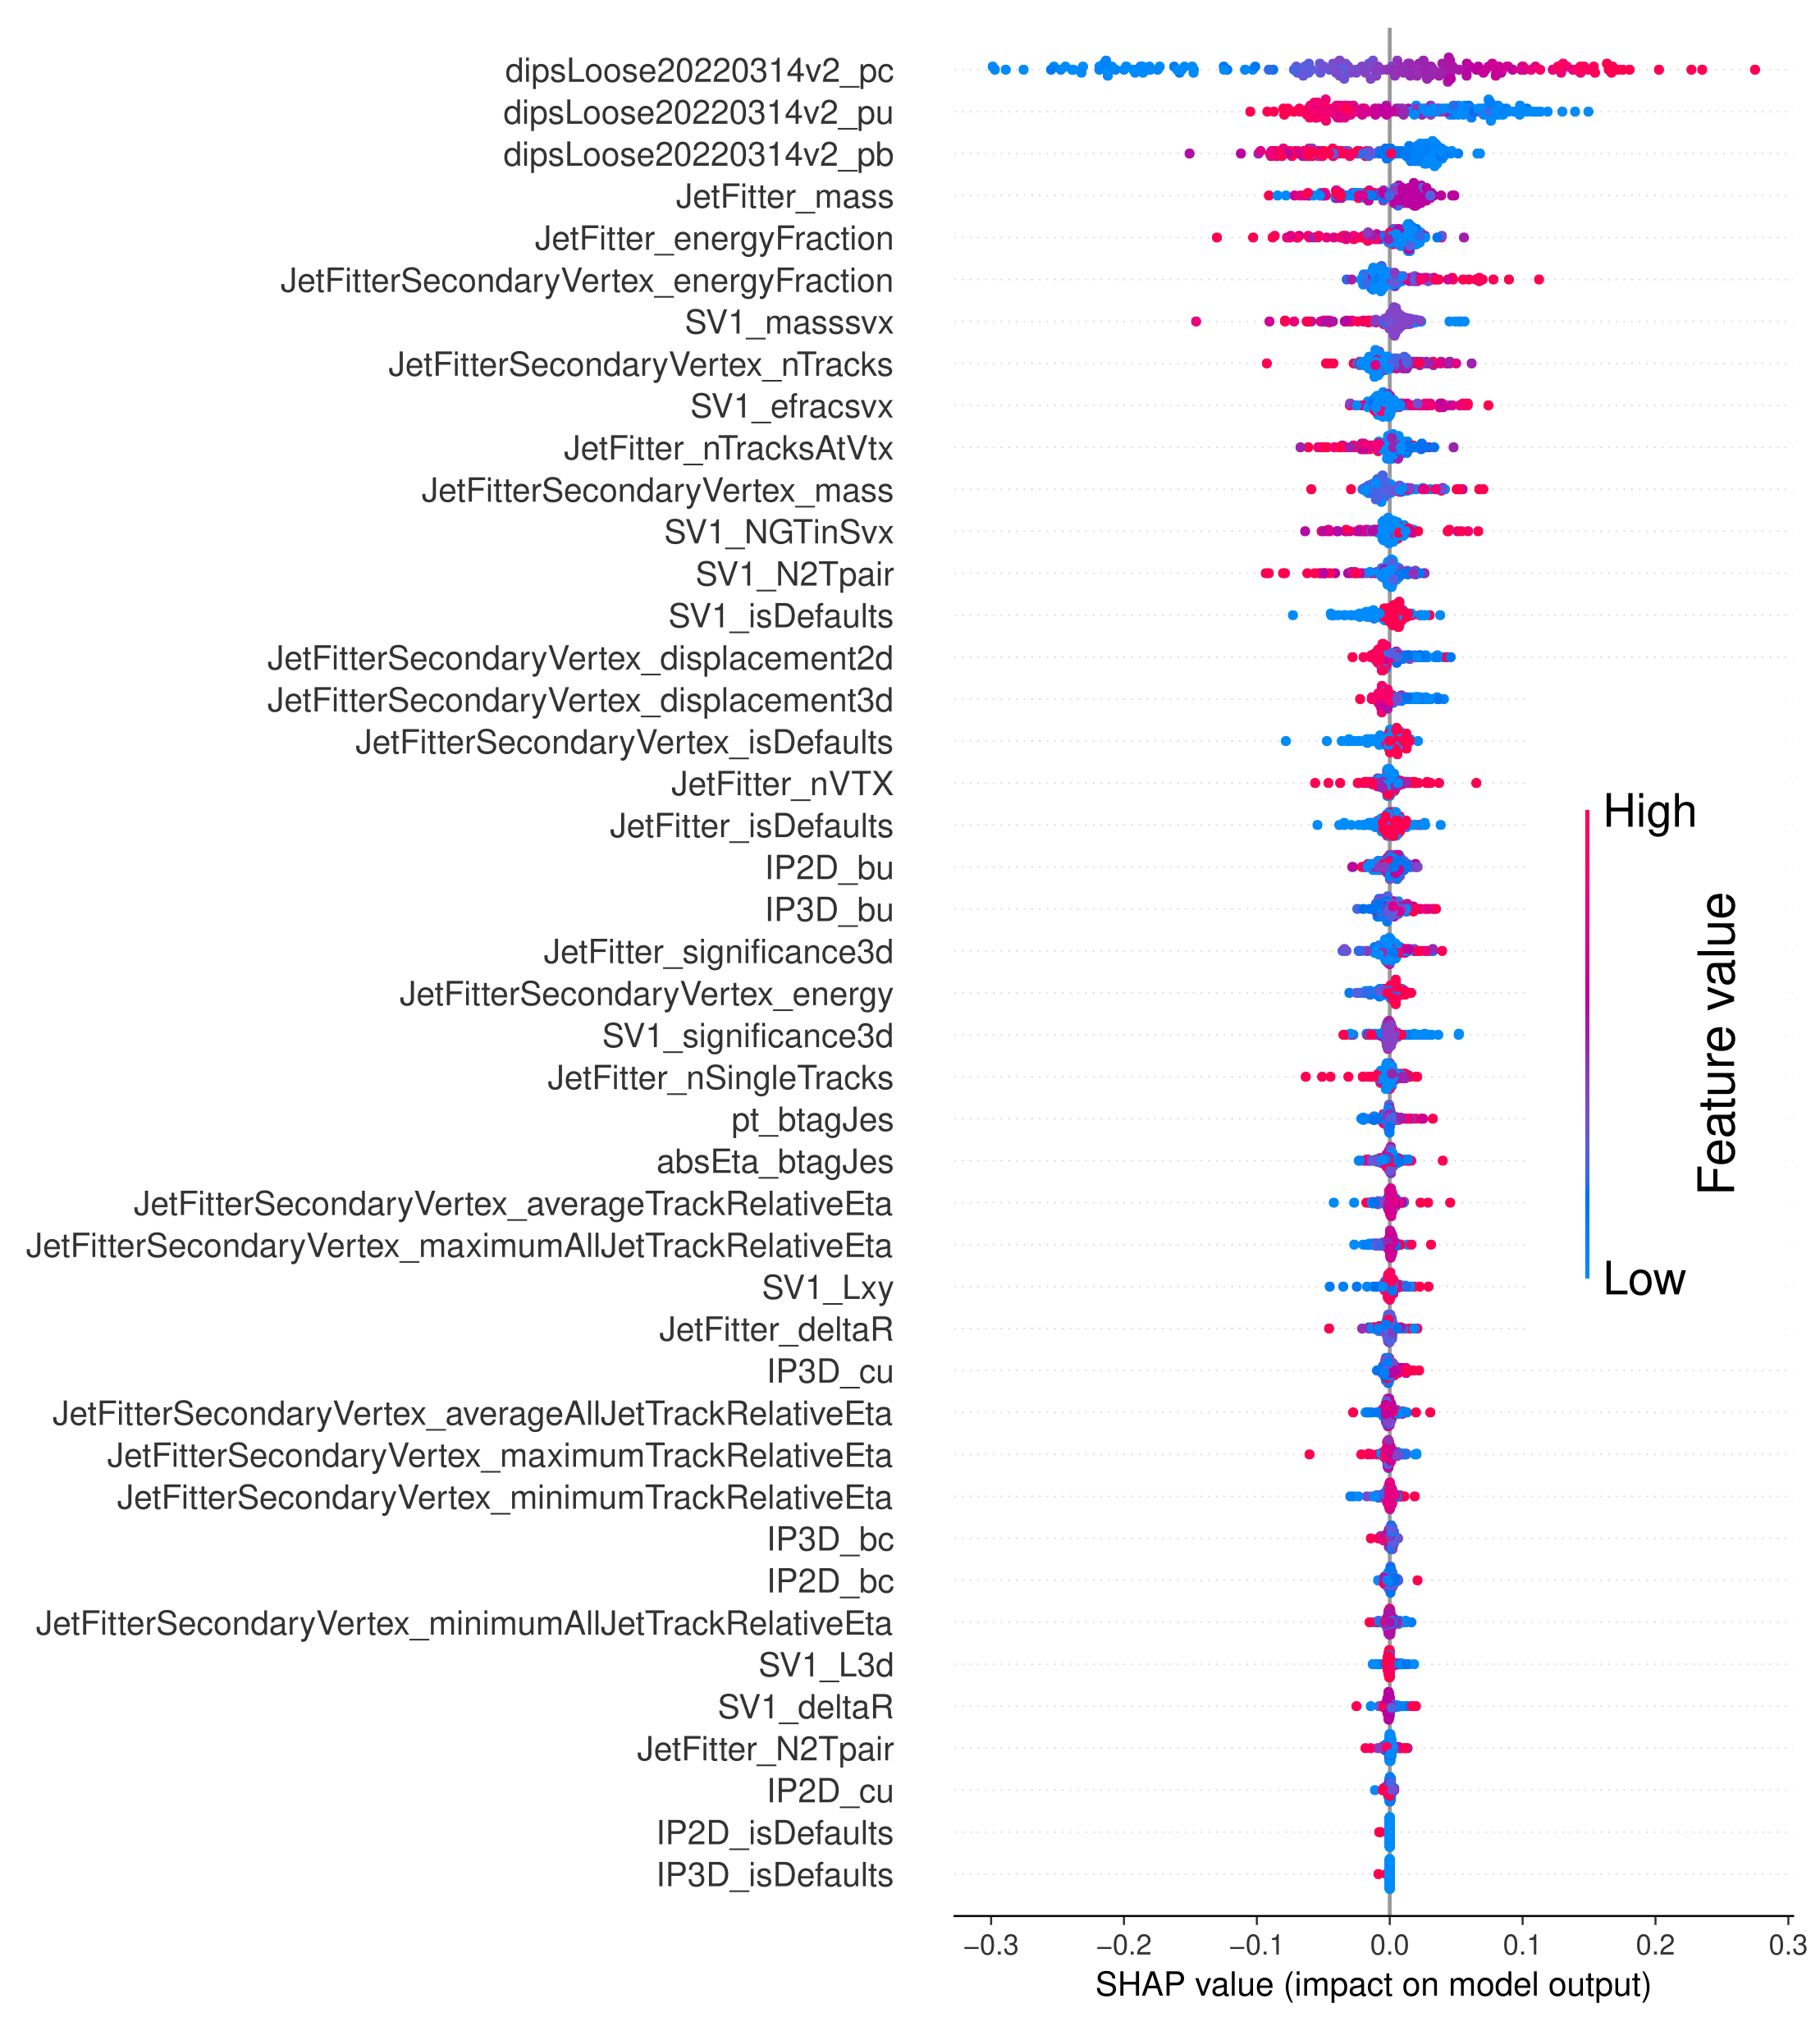
\includegraphics[scale=0.7]{Images/FTAG/DL1d/Shap/ttc.png}
  \includegraphics[scale=0.7]{Images/FTAG/DL1d/Shap/zpc.png}
  \caption{Shapley values of the different inputs variables of DL1d for $c$-tagging, $t\bar{t}$ on the left and $Z'$ on the right.} 
  \label{fig:DL1dshapc}
\end{sidewaysfigure} 

Inspecting Figure \ref{fig:DL1dshapb} reveals some interesting patterns in the \gls{dl1d} network for the task of $b$-tagging. The most important family of features for this task are the \gls{dips} probabilities, with higher values of $p_b$ correctly identifying the jet as $b$ while higher values of $p_c$ and $p_{\textrm{light}}$ (noted $p_u$) have the opposite effect. The number of 2-track pairs from \gls{sv1} and some JetFitter variables - namely the mass of the vertex, the energy fraction and the number of tracks at the vertex - are also highlighted as important features. These observations are in line with the physics-based reasoning about the dynamic behind the jet: $b$-jets are expected to have a large charged particle multiplicity and the exchange of momentum is hard, with the $b$-hadron taking most of the $b$-quark momentum. Some other interesting features to consider are the ones formatted as  ``algoName\_isDefaults'': they track whether the base-method ``algoName'' is activated (0 - blue) or not and thus defaulting (1 - red) for each jet. Interestingly, most of the occurences of a defaulting behaviour of \gls{sv1} and JetFitter are associated with a negative Shapley values, demonstrating the validaty of the physics-reasoning behind these methods and their active contributions to $b$-tagging. IPxD variables generally score low in the ranking, indicating these methods contribute little to the model predictions and can be safely removed, an observation confirmed by direct searches over the input features set. Contrasting the Shapley values for $t\bar{t}$ (left) and $Z'$ (right), the same variables roughly rank in the same order with minimal differences explained by the change in kinematic phase space between the two samples. \\

The same analysis can be carried out for $c$-tagging, with the results displayed in Figure \ref{fig:DL1dshapc}. As discussed for $b$-tagging, the most important features are again the \gls{dips} probabilities with $p_c$ ranking first and contributing the most to $D_c$. Interestingly, the ranking of features is roughly the same as for $D_b$, with most features that had a positive impact on $D_b$ when taking larger values now having a negative impact on $D_c$. This is the case of most of the JetFitter and \gls{sv1} variables. Defaulting behaviour of these algorithms, occuring when the conditions of a jet do not pass certain requirements, often has a positive effect on $D_c$ as expected. Again, the IPxD family of features score low, indicating the limited importance of their contributions to the output. 

\subsection{Training of DL1d on Variable Radius Jets for Run 3}\label{sec:VRdl1dTrain}
As for \gls{dips}, changing the jet definition from PFlow to \gls{vr}-jets is expected to have a large impact on the performance of the methods described here. Building on from the \gls{vr}-trained \gls{dips} model introduced in Section \ref{chapter:dipsVRtrain}, this section presents the training of \gls{dl1d} for \gls{vr}-jets. The datasets are similar to those of Section \ref{chapter:dipsVRtrain}. The \gls{vr}-trained \gls{dl1d} was trained for 300 epochs with no signs of overtraining. Its performance here is compared to the PFlow version introduced in the previous section, as well as the R21 \gls{dl1r} version trained on \gls{vr}-jets too and a pre-release \gls{gn1} trained on 20 million \gls{vr}-jets.

\begin{sidewaysfigure}
  \vspace{0.6cm}
  %\hspace{0.5cm}
  \begin{subfigure}[t]{0.3\textwidth}
    \centering
    \includegraphics[scale=0.43]{Images/FTAG/VRDL1d/ROC/ttb.png}
    \caption{$t\bar{t}$ test sample $b$-tagging, $f_c = 0.018$ for DL1d.}
    \label{fig:dl1dVRROCtt}
  \end{subfigure}
  \hfill
  \begin{subfigure}[t]{0.3\textwidth}
    \centering
    \includegraphics[scale=0.43]{Images/FTAG/VRDL1d/ROC/zpb.png}
    \caption{$Z'$ test sample $b$-tagging, $f_c = 0.018$ for DL1d.}
    \label{fig:dl1dVRROCzp}
  \end{subfigure}
  \hfill
  \begin{subfigure}[t]{0.3\textwidth}
    \centering
    \includegraphics[scale=0.43]{Images/FTAG/VRDL1d/ROC/grb.png}
    \caption{Graviton sample $b$-tagging, $f_c = 0.018$ for DL1d.}
    \label{fig:dl1dVRROCgr}
  \end{subfigure} \\
  \begin{subfigure}[t]{0.3\textwidth}
    \centering
    \includegraphics[scale=0.43]{Images/FTAG/VRDL1d/ROC/ttbupf.png}
    \caption{$t\bar{t}$ test sample $b$-tagging, $f_c = 0.1$ for DL1d.}
    \label{fig:dl1dVRROCttc}
  \end{subfigure}
  \hfill
  \begin{subfigure}[t]{0.3\textwidth}
    \centering
    \includegraphics[scale=0.43]{Images/FTAG/VRDL1d/ROC/zpbupf.png}
    \caption{$Z'$ test sample $b$-tagging, $f_c = 0.1$ for DL1d.}
    \label{fig:dl1dVRROCzpc}
  \end{subfigure}
  \hfill
  \begin{subfigure}[t]{0.3\textwidth}
    \centering
    \includegraphics[scale=0.43]{Images/FTAG/VRDL1d/ROC/grbupf.png}
    \caption{Graviton sample $b$-tagging, $f_c = 0.1$ for DL1d.}
    \label{fig:dl1dVRROCgrc}
  \end{subfigure}
  \caption{\gls{roc} curves for $b$-tagging for $t\bar{t}$ (left), $Z'$ (centre), and graviton (right)processes. Top row uses $f_c = 0.018$ for DL1d, while bottom row is $f_c = 0.1$ (GN1 $f_c = 0.05$ everywhere). Models are displayed as curves of different colours, with the \gls{vr}-jets \gls{dl1d} in blue, a pre-release \gls{vr}-trained \gls{gn1} on 20 million in orange, \gls{dl1r} trained on \gls{vr}-jets with the previous software release R21 in green, and the PFlow trained \gls{dl1d} in red.}
  \label{fig:dl1dVRROC}
\end{sidewaysfigure}

A clear benefit from retraining on the dedicated \gls{vr}-jet sets is observed on the \gls{roc} curves, with the \gls{vr}-\gls{dl1d} outperforming the PFlow version for all $b$- and $c$-tagging efficiencies considered. Introducing \gls{dips} in the \gls{dl1} architecture has a significant impact on the performance of the tagger and greatly overmatches the \gls{rnnip} contribution. This is further highlighted by Table \ref{tab:max-perf-dl1dVR} reporting the rejections obtained at different \gls{wp} of typical interest in analyses.

\begin{table}[h]
  \begin{center}
      \begin{tabular}{C{1.5cm}|cc|cc|cc} 
      	 \hline \hline
          \multicolumn{7}{c}{$b$-tagging}\\ \hline
          & \multicolumn{2}{c|}{$t\bar{t}$} & \multicolumn{2}{c|}{$Z'$} & \multicolumn{2}{c}{Graviton} \\
          WP & $c$-rej  & light-rej & $c$-rej  & light-rej & $c$-rej  & light-rej  \\ \hline
          60\%  & +20\% &  +6\% & +14\% & +83\% & +19\% & +72\%  \\ 
          70\%  & +18\% &  +9\% & +14\% & +65\% & +16\% & +57\%  \\ 
          77\%  & +13\% & +15\% & +13\% & +56\% & +14\% & +51\%  \\ 
          85\%  &  +1\% & +25\% & +11\% & +45\% & +12\% & +40\%  \\ \hline
          \multicolumn{3}{c}{} \\
           \hline  \hline
           \multicolumn{7}{c}{$c$-tagging}\\ \hline
          & \multicolumn{2}{c|}{$t\bar{t}$} & \multicolumn{2}{c|}{$Z'$} & \multicolumn{2}{c}{Graviton} \\ 
          WP & $b$-rej  & light-rej & $b$-rej  & light-rej & $b$-rej  & light-rej  \\ \hline
          25\%   & -20\% & +137\% & -17\% & +90\% & -17\% & +80\% \\
          30\%   & -25\% & +114\% & -21\% & +73\% & -19\% & +66\% \\
          40\%   & -29\% &  +99\% & -23\% & +53\% & -22\% & +48\% \\
          50\%   & -29\% &  +80\% & -24\% & +39\% & -22\% & +35\% \\ \hline \hline
      \end{tabular}
    \caption{The change in background flavour rejection of \gls{vr}-trained \gls{dl1d} relative to the PFlow trained \gls{dl1d} at various tagging efficiencies, both trained on the new release. Top: $b$-tagging ($f^b_c = 0.1$ and 0.018 for the \gls{vr} and PFlow trainijng); bottom: $c$-tagging ($f^c_b = 0.2$); left: $t\bar{t}$; centre: $Z'$, left: graviton.}
    \label{tab:max-perf-dl1dVR}
  \end{center}
\end{table}

As shown in Table \ref{tab:max-perf-dl1dVR}, the new \gls{vr}-trained \gls{dl1d} is found to outperform the PFlow version with the flavour fraction parameter for $b$-tagging $f^b_c$ changed from 0.018 (for PFlow) to 0.1. For $c$-tagging, a clear gain in light-rejection comes at a cost of $b$-rejection which can also be corrected by an appropriate change of the flavour fraction parameter for $c$-tagging $f^c_b$, currently set at 0.2. As concluded in Figure \ref{apfig:DL1dVRscanf} of Appendix \ref{ap-DL1dVR}, which displays flavour fractions scans for $b$- and $c$-tagging, this choice of $f^c_b$ is not optimal for the 30\% \gls{wp}. \\

While this physics-motivated architecture optimisation moving from an \gls{rnn}-based to a Deep Set-based track analyser improves the efficiency of the hieararchical model, a clear gain in performance is accessible throught a more radical modification of the architecture as is done with the \gls{gn1} model. This is a classical observation in the world of machine learning: vast amount of low-level noisy data can be better exploited by sophisticated architecture than by using a simple model fed a few highly engineered and reconstructed features, even when these are physically motivated. \gls{gn1} is not based on any physics principles. As will be shown in the next section, tracks themselves contain enough of the rich physics signature required to unlock the label of the jet they compose. 
